\documentclass[twoside]{book}

% Packages required by doxygen
\usepackage{fixltx2e}
\usepackage{calc}
\usepackage{doxygen}
\usepackage[export]{adjustbox} % also loads graphicx
\usepackage{graphicx}
\usepackage[utf8]{inputenc}
\usepackage{makeidx}
\usepackage{multicol}
\usepackage{multirow}
\PassOptionsToPackage{warn}{textcomp}
\usepackage{textcomp}
\usepackage[nointegrals]{wasysym}
\usepackage[table]{xcolor}

% Font selection
\usepackage[T1]{fontenc}
\usepackage[scaled=.90]{helvet}
\usepackage{courier}
\usepackage{amssymb}
\usepackage{sectsty}
\renewcommand{\familydefault}{\sfdefault}
\allsectionsfont{%
  \fontseries{bc}\selectfont%
  \color{darkgray}%
}
\renewcommand{\DoxyLabelFont}{%
  \fontseries{bc}\selectfont%
  \color{darkgray}%
}
\newcommand{\+}{\discretionary{\mbox{\scriptsize$\hookleftarrow$}}{}{}}

% Page & text layout
\usepackage{geometry}
\geometry{%
  a4paper,%
  top=2.5cm,%
  bottom=2.5cm,%
  left=2.5cm,%
  right=2.5cm%
}
\tolerance=750
\hfuzz=15pt
\hbadness=750
\setlength{\emergencystretch}{15pt}
\setlength{\parindent}{0cm}
\setlength{\parskip}{3ex plus 2ex minus 2ex}
\makeatletter
\renewcommand{\paragraph}{%
  \@startsection{paragraph}{4}{0ex}{-1.0ex}{1.0ex}{%
    \normalfont\normalsize\bfseries\SS@parafont%
  }%
}
\renewcommand{\subparagraph}{%
  \@startsection{subparagraph}{5}{0ex}{-1.0ex}{1.0ex}{%
    \normalfont\normalsize\bfseries\SS@subparafont%
  }%
}
\makeatother

% Headers & footers
\usepackage{fancyhdr}
\pagestyle{fancyplain}
\fancyhead[LE]{\fancyplain{}{\bfseries\thepage}}
\fancyhead[CE]{\fancyplain{}{}}
\fancyhead[RE]{\fancyplain{}{\bfseries\leftmark}}
\fancyhead[LO]{\fancyplain{}{\bfseries\rightmark}}
\fancyhead[CO]{\fancyplain{}{}}
\fancyhead[RO]{\fancyplain{}{\bfseries\thepage}}
\fancyfoot[LE]{\fancyplain{}{}}
\fancyfoot[CE]{\fancyplain{}{}}
\fancyfoot[RE]{\fancyplain{}{\bfseries\scriptsize Generated by Doxygen }}
\fancyfoot[LO]{\fancyplain{}{\bfseries\scriptsize Generated by Doxygen }}
\fancyfoot[CO]{\fancyplain{}{}}
\fancyfoot[RO]{\fancyplain{}{}}
\renewcommand{\footrulewidth}{0.4pt}
\renewcommand{\chaptermark}[1]{%
  \markboth{#1}{}%
}
\renewcommand{\sectionmark}[1]{%
  \markright{\thesection\ #1}%
}

% Indices & bibliography
\usepackage{natbib}
\usepackage[titles]{tocloft}
\setcounter{tocdepth}{3}
\setcounter{secnumdepth}{5}
\makeindex

% Hyperlinks (required, but should be loaded last)
\usepackage{ifpdf}
\ifpdf
  \usepackage[pdftex,pagebackref=true]{hyperref}
\else
  \usepackage[ps2pdf,pagebackref=true]{hyperref}
\fi
\hypersetup{%
  colorlinks=true,%
  linkcolor=blue,%
  citecolor=blue,%
  unicode%
}

% Custom commands
\newcommand{\clearemptydoublepage}{%
  \newpage{\pagestyle{empty}\cleardoublepage}%
}

\usepackage{caption}
\captionsetup{labelsep=space,justification=centering,font={bf},singlelinecheck=off,skip=4pt,position=top}

%===== C O N T E N T S =====

\begin{document}

% Titlepage & ToC
\hypersetup{pageanchor=false,
             bookmarksnumbered=true,
             pdfencoding=unicode
            }
\pagenumbering{alph}
\begin{titlepage}
\vspace*{7cm}
\begin{center}%
{\Large Flex\+Box -\/ A Flexible Primal-\/\+Dual Tool\+Box }\\
\vspace*{1cm}
{\large Generated by Doxygen 1.8.13}\\
\end{center}
\end{titlepage}
\clearemptydoublepage
\pagenumbering{roman}
\tableofcontents
\clearemptydoublepage
\pagenumbering{arabic}
\hypersetup{pageanchor=true}

%--- Begin generated contents ---
\chapter{Main Page}
\label{index}\hypertarget{index}{}\hypertarget{index_intro_sec}{}\section{Introduction}\label{index_intro_sec}
Flex\+Box is a flexible M\+A\+T\+L\+AB toolbox for finite dimensional convex variational problems in image processing and beyond. Such problems often consist of non-\/differentiable parts and involve linear operators. The toolbox uses a primal-\/dual scheme to avoid (computationally) inefficient operator inversion and to get reliable error estimates. From the user-\/side, Flex\+Box expects the primal formulation of the problem, automatically decouples operators and dualizes the problem. For large-\/scale problems, Flex\+Box also comes with a C++ modulke, which can be used stand-\/alone or together with M\+A\+T\+L\+AB via M\+E\+X-\/interfaces. Besides various pre-\/implemented data-\/fidelities and regularization-\/terms, Flex\+Box is able to handle arbitrary operators while being easily extendable, due to its object-\/oriented design. The toolbox is available at \href{http://www.flexbox.im}{\tt http\+://www.\+flexbox.\+im}

Nowadays, many problems in image processing consist of minimizing convex energies. Typically these problems can be written as $\min_{x} F(Ax)$ 
\chapter{Hierarchical Index}
\section{Class Hierarchy}
This inheritance list is sorted roughly, but not completely, alphabetically\+:\begin{DoxyCompactList}
\item \contentsline{section}{files}{\pageref{structfiles}}{}
\item \contentsline{section}{flex\+Prox\+Dual\+L2\+Inf$<$ T $>$\+:\+:Find\+Transform}{\pageref{structflex_prox_dual_l2_inf_1_1_find_transform}}{}
\item \contentsline{section}{flex\+Box$<$ T $>$}{\pageref{classflex_box}}{}
\item \contentsline{section}{flex\+Box\+Data$<$ T $>$}{\pageref{classflex_box_data}}{}
\begin{DoxyCompactList}
\item \contentsline{section}{flex\+Box\+Data\+C\+PU$<$ T $>$}{\pageref{classflex_box_data_c_p_u}}{}
\item \contentsline{section}{flex\+Box\+Data\+G\+PU$<$ T $>$}{\pageref{classflex_box_data_g_p_u}}{}
\end{DoxyCompactList}
\item \contentsline{section}{flex\+Linear\+Operator$<$ T $>$}{\pageref{classflex_linear_operator}}{}
\begin{DoxyCompactList}
\item \contentsline{section}{flex\+Concat\+Operator$<$ T $>$}{\pageref{classflex_concat_operator}}{}
\item \contentsline{section}{flex\+Diagonal\+Operator$<$ T $>$}{\pageref{classflex_diagonal_operator}}{}
\item \contentsline{section}{flex\+Full\+Matrix$<$ T $>$}{\pageref{classflex_full_matrix}}{}
\item \contentsline{section}{flex\+Gradient\+Operator$<$ T $>$}{\pageref{classflex_gradient_operator}}{}
\item \contentsline{section}{flex\+Identity\+Operator$<$ T $>$}{\pageref{classflex_identity_operator}}{}
\item \contentsline{section}{flex\+Matrix$<$ T $>$}{\pageref{classflex_matrix}}{}
\item \contentsline{section}{flex\+Matrix\+G\+PU$<$ T $>$}{\pageref{classflex_matrix_g_p_u}}{}
\item \contentsline{section}{flex\+Matrix\+Logical$<$ T $>$}{\pageref{classflex_matrix_logical}}{}
\item \contentsline{section}{flex\+Superpixel\+Operator$<$ T $>$}{\pageref{classflex_superpixel_operator}}{}
\item \contentsline{section}{flex\+Zero\+Operator$<$ T $>$}{\pageref{classflex_zero_operator}}{}
\end{DoxyCompactList}
\item \contentsline{section}{flex\+Prox$<$ T $>$}{\pageref{classflex_prox}}{}
\begin{DoxyCompactList}
\item \contentsline{section}{flex\+Prox\+Dual\+Box\+Constraint$<$ T $>$}{\pageref{classflex_prox_dual_box_constraint}}{}
\item \contentsline{section}{flex\+Prox\+Dual\+Data\+Huber$<$ T $>$}{\pageref{classflex_prox_dual_data_huber}}{}
\item \contentsline{section}{flex\+Prox\+Dual\+Data\+KL$<$ T $>$}{\pageref{classflex_prox_dual_data_k_l}}{}
\item \contentsline{section}{flex\+Prox\+Dual\+Data\+L1$<$ T $>$}{\pageref{classflex_prox_dual_data_l1}}{}
\item \contentsline{section}{flex\+Prox\+Dual\+Data\+L2$<$ T $>$}{\pageref{classflex_prox_dual_data_l2}}{}
\item \contentsline{section}{flex\+Prox\+Dual\+Frobenius$<$ T $>$}{\pageref{classflex_prox_dual_frobenius}}{}
\item \contentsline{section}{flex\+Prox\+Dual\+Huber$<$ T $>$}{\pageref{classflex_prox_dual_huber}}{}
\item \contentsline{section}{flex\+Prox\+Dual\+Inner\+Product$<$ T $>$}{\pageref{classflex_prox_dual_inner_product}}{}
\item \contentsline{section}{flex\+Prox\+Dual\+L1\+Aniso$<$ T $>$}{\pageref{classflex_prox_dual_l1_aniso}}{}
\item \contentsline{section}{flex\+Prox\+Dual\+L1\+Iso$<$ T $>$}{\pageref{classflex_prox_dual_l1_iso}}{}
\item \contentsline{section}{flex\+Prox\+Dual\+L2$<$ T $>$}{\pageref{classflex_prox_dual_l2}}{}
\item \contentsline{section}{flex\+Prox\+Dual\+L2\+Inf$<$ T $>$}{\pageref{classflex_prox_dual_l2_inf}}{}
\item \contentsline{section}{flex\+Prox\+Dual\+Labeling$<$ T $>$}{\pageref{classflex_prox_dual_labeling}}{}
\item \contentsline{section}{flex\+Prox\+Dual\+L\+Inf$<$ T $>$}{\pageref{classflex_prox_dual_l_inf}}{}
\end{DoxyCompactList}
\item \contentsline{section}{flex\+Solver$<$ T $>$}{\pageref{classflex_solver}}{}
\begin{DoxyCompactList}
\item \contentsline{section}{flex\+Solver\+Primal\+Dual$<$ T $>$}{\pageref{classflex_solver_primal_dual}}{}
\item \contentsline{section}{flex\+Solver\+Primal\+Dual\+Cuda$<$ T $>$}{\pageref{classflex_solver_primal_dual_cuda}}{}
\end{DoxyCompactList}
\item \contentsline{section}{flex\+Term$<$ T $>$}{\pageref{classflex_term}}{}
\item \contentsline{section}{flex\+Prox\+Dual\+L2\+Inf$<$ T $>$\+:\+:Greater\+Equal\+Zero}{\pageref{structflex_prox_dual_l2_inf_1_1_greater_equal_zero}}{}
\item \contentsline{section}{flex\+Prox\+Dual\+L2\+Inf$<$ T $>$\+:\+:L21\+Norm\+Dim2}{\pageref{structflex_prox_dual_l2_inf_1_1_l21_norm_dim2}}{}
\item \contentsline{section}{flex\+Prox\+Dual\+L2\+Inf$<$ T $>$\+:\+:L21\+Norm\+Dim3}{\pageref{structflex_prox_dual_l2_inf_1_1_l21_norm_dim3}}{}
\item \contentsline{section}{my\+Abs\+G\+PU$<$ T $>$}{\pageref{structmy_abs_g_p_u}}{}
\item \contentsline{section}{Timer}{\pageref{class_timer}}{}
\item \contentsline{section}{vector\+Add\+Vector\+Times\+Vector\+G\+PU}{\pageref{structvector_add_vector_times_vector_g_p_u}}{}
\end{DoxyCompactList}

\chapter{Class Index}
\section{Class List}
Here are the classes, structs, unions and interfaces with brief descriptions\+:\begin{DoxyCompactList}
\item\contentsline{section}{\hyperlink{structfiles}{files} }{\pageref{structfiles}}{}
\item\contentsline{section}{\hyperlink{structflex_prox_dual_l2_inf_1_1_find_transform}{flex\+Prox\+Dual\+L2\+Inf$<$ T $>$\+::\+Find\+Transform} }{\pageref{structflex_prox_dual_l2_inf_1_1_find_transform}}{}
\item\contentsline{section}{\hyperlink{classflex_box}{flex\+Box$<$ T $>$} \\*Flex\+Box main class }{\pageref{classflex_box}}{}
\item\contentsline{section}{\hyperlink{classflex_box_data}{flex\+Box\+Data$<$ T $>$} \\*Flex\+Box data class }{\pageref{classflex_box_data}}{}
\item\contentsline{section}{\hyperlink{classflex_box_data_c_p_u}{flex\+Box\+Data\+C\+P\+U$<$ T $>$} \\*Flex\+Box data class if using the non-\/\+C\+U\+DA version }{\pageref{classflex_box_data_c_p_u}}{}
\item\contentsline{section}{\hyperlink{classflex_box_data_g_p_u}{flex\+Box\+Data\+G\+P\+U$<$ T $>$} \\*Flex\+Box data class if using the C\+U\+DA }{\pageref{classflex_box_data_g_p_u}}{}
\item\contentsline{section}{\hyperlink{classflex_concat_operator}{flex\+Concat\+Operator$<$ T $>$} \\*Concatenation operator }{\pageref{classflex_concat_operator}}{}
\item\contentsline{section}{\hyperlink{classflex_diagonal_operator}{flex\+Diagonal\+Operator$<$ T $>$} \\*Diagonal operator }{\pageref{classflex_diagonal_operator}}{}
\item\contentsline{section}{\hyperlink{classflex_full_matrix}{flex\+Full\+Matrix$<$ T $>$} \\*Full (non-\/\+C\+U\+DA) matrix }{\pageref{classflex_full_matrix}}{}
\item\contentsline{section}{\hyperlink{classflex_gradient_operator}{flex\+Gradient\+Operator$<$ T $>$} \\*Gradient operator }{\pageref{classflex_gradient_operator}}{}
\item\contentsline{section}{\hyperlink{classflex_identity_operator}{flex\+Identity\+Operator$<$ T $>$} \\*Identiy operator }{\pageref{classflex_identity_operator}}{}
\item\contentsline{section}{\hyperlink{classflex_linear_operator}{flex\+Linear\+Operator$<$ T $>$} \\*Abstract base class for linear operators }{\pageref{classflex_linear_operator}}{}
\item\contentsline{section}{\hyperlink{classflex_matrix}{flex\+Matrix$<$ T $>$} \\*(non-\/\+C\+U\+DA) matrix }{\pageref{classflex_matrix}}{}
\item\contentsline{section}{\hyperlink{classflex_matrix_g_p_u}{flex\+Matrix\+G\+P\+U$<$ T $>$} \\*(C\+U\+DA) matrix }{\pageref{classflex_matrix_g_p_u}}{}
\item\contentsline{section}{\hyperlink{classflex_matrix_logical}{flex\+Matrix\+Logical$<$ T $>$} \\*Full (non-\/\+C\+U\+DA) logical matrix }{\pageref{classflex_matrix_logical}}{}
\item\contentsline{section}{\hyperlink{classflex_prox}{flex\+Prox$<$ T $>$} \\*Abstract base class for all proximals (prox) }{\pageref{classflex_prox}}{}
\item\contentsline{section}{\hyperlink{classflex_prox_dual_box_constraint}{flex\+Prox\+Dual\+Box\+Constraint$<$ T $>$} \\*Prox for a box constraint }{\pageref{classflex_prox_dual_box_constraint}}{}
\item\contentsline{section}{\hyperlink{classflex_prox_dual_data_huber}{flex\+Prox\+Dual\+Data\+Huber$<$ T $>$} \\*Prox for a Huber data term }{\pageref{classflex_prox_dual_data_huber}}{}
\item\contentsline{section}{\hyperlink{classflex_prox_dual_data_k_l}{flex\+Prox\+Dual\+Data\+K\+L$<$ T $>$} \\*Prox for a Kullback-\/\+Leibler divergence data term }{\pageref{classflex_prox_dual_data_k_l}}{}
\item\contentsline{section}{\hyperlink{classflex_prox_dual_data_l1}{flex\+Prox\+Dual\+Data\+L1$<$ T $>$} \\*Prox for a L1 data term }{\pageref{classflex_prox_dual_data_l1}}{}
\item\contentsline{section}{\hyperlink{classflex_prox_dual_data_l2}{flex\+Prox\+Dual\+Data\+L2$<$ T $>$} \\*Prox for a L2 data term }{\pageref{classflex_prox_dual_data_l2}}{}
\item\contentsline{section}{\hyperlink{classflex_prox_dual_frobenius}{flex\+Prox\+Dual\+Frobenius$<$ T $>$} \\*Prox for a Frobenius term }{\pageref{classflex_prox_dual_frobenius}}{}
\item\contentsline{section}{\hyperlink{classflex_prox_dual_huber}{flex\+Prox\+Dual\+Huber$<$ T $>$} \\*Prox for a Huber term }{\pageref{classflex_prox_dual_huber}}{}
\item\contentsline{section}{\hyperlink{classflex_prox_dual_inner_product}{flex\+Prox\+Dual\+Inner\+Product$<$ T $>$} \\*Prox for an inner product data term }{\pageref{classflex_prox_dual_inner_product}}{}
\item\contentsline{section}{\hyperlink{classflex_prox_dual_l1_aniso}{flex\+Prox\+Dual\+L1\+Aniso$<$ T $>$} \\*Prox for a L1 non-\/data term }{\pageref{classflex_prox_dual_l1_aniso}}{}
\item\contentsline{section}{\hyperlink{classflex_prox_dual_l1_iso}{flex\+Prox\+Dual\+L1\+Iso$<$ T $>$} \\*Prox for a L1 non-\/data term }{\pageref{classflex_prox_dual_l1_iso}}{}
\item\contentsline{section}{\hyperlink{classflex_prox_dual_l2}{flex\+Prox\+Dual\+L2$<$ T $>$} \\*Prox for a L2 non-\/data term }{\pageref{classflex_prox_dual_l2}}{}
\item\contentsline{section}{\hyperlink{classflex_prox_dual_l2_inf}{flex\+Prox\+Dual\+L2\+Inf$<$ T $>$} \\*Prox for a L2,inf non-\/data term }{\pageref{classflex_prox_dual_l2_inf}}{}
\item\contentsline{section}{\hyperlink{classflex_prox_dual_labeling}{flex\+Prox\+Dual\+Labeling$<$ T $>$} \\*Prox for a labeling term }{\pageref{classflex_prox_dual_labeling}}{}
\item\contentsline{section}{\hyperlink{classflex_prox_dual_l_inf}{flex\+Prox\+Dual\+L\+Inf$<$ T $>$} \\*Prox for a L\+Inf non-\/data term }{\pageref{classflex_prox_dual_l_inf}}{}
\item\contentsline{section}{\hyperlink{classflex_solver}{flex\+Solver$<$ T $>$} \\*Flex\+Box solver class }{\pageref{classflex_solver}}{}
\item\contentsline{section}{\hyperlink{classflex_solver_primal_dual}{flex\+Solver\+Primal\+Dual$<$ T $>$} \\*Flex\+Box solver class if using the non-\/\+C\+U\+DA version }{\pageref{classflex_solver_primal_dual}}{}
\item\contentsline{section}{\hyperlink{classflex_solver_primal_dual_cuda}{flex\+Solver\+Primal\+Dual\+Cuda$<$ T $>$} \\*Flex\+Box solver class if using the C\+U\+DA version }{\pageref{classflex_solver_primal_dual_cuda}}{}
\item\contentsline{section}{\hyperlink{classflex_superpixel_operator}{flex\+Superpixel\+Operator$<$ T $>$} \\*Superpixel operator }{\pageref{classflex_superpixel_operator}}{}
\item\contentsline{section}{\hyperlink{classflex_term}{flex\+Term$<$ T $>$} \\*Wrapper class for all usable terms }{\pageref{classflex_term}}{}
\item\contentsline{section}{\hyperlink{classflex_zero_operator}{flex\+Zero\+Operator$<$ T $>$} \\*Zero operator (empty matrix) }{\pageref{classflex_zero_operator}}{}
\item\contentsline{section}{\hyperlink{structflex_prox_dual_l2_inf_1_1_greater_equal_zero}{flex\+Prox\+Dual\+L2\+Inf$<$ T $>$\+::\+Greater\+Equal\+Zero} }{\pageref{structflex_prox_dual_l2_inf_1_1_greater_equal_zero}}{}
\item\contentsline{section}{\hyperlink{structflex_prox_dual_l2_inf_1_1_l21_norm_dim2}{flex\+Prox\+Dual\+L2\+Inf$<$ T $>$\+::\+L21\+Norm\+Dim2} }{\pageref{structflex_prox_dual_l2_inf_1_1_l21_norm_dim2}}{}
\item\contentsline{section}{\hyperlink{structflex_prox_dual_l2_inf_1_1_l21_norm_dim3}{flex\+Prox\+Dual\+L2\+Inf$<$ T $>$\+::\+L21\+Norm\+Dim3} }{\pageref{structflex_prox_dual_l2_inf_1_1_l21_norm_dim3}}{}
\item\contentsline{section}{\hyperlink{structmy_abs_g_p_u}{my\+Abs\+G\+P\+U$<$ T $>$} \\*Thrust functor for calculating the absolute value of vector }{\pageref{structmy_abs_g_p_u}}{}
\item\contentsline{section}{\hyperlink{class_timer}{Timer} \\*Class for timing execution times }{\pageref{class_timer}}{}
\item\contentsline{section}{\hyperlink{structvector_add_vector_times_vector_g_p_u}{vector\+Add\+Vector\+Times\+Vector\+G\+PU} \\*Thrust functor for elemntwise multiplication of two vectors following a summation of the result on a third vector }{\pageref{structvector_add_vector_times_vector_g_p_u}}{}
\end{DoxyCompactList}

\chapter{File Index}
\section{File List}
Here is a list of all documented files with brief descriptions\+:\begin{DoxyCompactList}
\item\contentsline{section}{{\bfseries flex\+Box.\+h} }{\pageref{flex_box_8h}}{}
\item\contentsline{section}{{\bfseries flex\+Box\+Data.\+h} }{\pageref{flex_box_data_8h}}{}
\item\contentsline{section}{{\bfseries flex\+Box\+Data\+C\+P\+U.\+h} }{\pageref{flex_box_data_c_p_u_8h}}{}
\item\contentsline{section}{{\bfseries flex\+Box\+Data\+G\+P\+U.\+h} }{\pageref{flex_box_data_g_p_u_8h}}{}
\item\contentsline{section}{{\bfseries flex\+Concat\+Operator.\+h} }{\pageref{flex_concat_operator_8h}}{}
\item\contentsline{section}{{\bfseries flex\+Diagonal\+Operator.\+h} }{\pageref{flex_diagonal_operator_8h}}{}
\item\contentsline{section}{{\bfseries flex\+Gradient\+Operator.\+h} }{\pageref{flex_gradient_operator_8h}}{}
\item\contentsline{section}{{\bfseries flex\+Identity\+Operator.\+h} }{\pageref{flex_identity_operator_8h}}{}
\item\contentsline{section}{{\bfseries flex\+Linear\+Operator.\+h} }{\pageref{flex_linear_operator_8h}}{}
\item\contentsline{section}{{\bfseries flex\+Matrix.\+h} }{\pageref{flex_matrix_8h}}{}
\item\contentsline{section}{{\bfseries flex\+Matrix\+G\+P\+U.\+h} }{\pageref{flex_matrix_g_p_u_8h}}{}
\item\contentsline{section}{{\bfseries flex\+Prox.\+h} }{\pageref{flex_prox_8h}}{}
\item\contentsline{section}{{\bfseries flex\+Prox\+Dual\+Box\+Constraint.\+h} }{\pageref{flex_prox_dual_box_constraint_8h}}{}
\item\contentsline{section}{{\bfseries flex\+Prox\+Dual\+Data\+K\+L.\+h} }{\pageref{flex_prox_dual_data_k_l_8h}}{}
\item\contentsline{section}{{\bfseries flex\+Prox\+Dual\+Data\+L1.\+h} }{\pageref{flex_prox_dual_data_l1_8h}}{}
\item\contentsline{section}{{\bfseries flex\+Prox\+Dual\+Data\+L2.\+h} }{\pageref{flex_prox_dual_data_l2_8h}}{}
\item\contentsline{section}{{\bfseries flex\+Prox\+Dual\+Frobenius.\+h} }{\pageref{flex_prox_dual_frobenius_8h}}{}
\item\contentsline{section}{{\bfseries flex\+Prox\+Dual\+Huber.\+h} }{\pageref{flex_prox_dual_huber_8h}}{}
\item\contentsline{section}{{\bfseries flex\+Prox\+Dual\+Inner\+Product.\+h} }{\pageref{flex_prox_dual_inner_product_8h}}{}
\item\contentsline{section}{{\bfseries flex\+Prox\+Dual\+L1\+Aniso.\+h} }{\pageref{flex_prox_dual_l1_aniso_8h}}{}
\item\contentsline{section}{{\bfseries flex\+Prox\+Dual\+L1\+Iso.\+h} }{\pageref{flex_prox_dual_l1_iso_8h}}{}
\item\contentsline{section}{{\bfseries flex\+Prox\+Dual\+L2.\+h} }{\pageref{flex_prox_dual_l2_8h}}{}
\item\contentsline{section}{{\bfseries flex\+Prox\+Dual\+Labeling.\+h} }{\pageref{flex_prox_dual_labeling_8h}}{}
\item\contentsline{section}{{\bfseries flex\+Solver.\+h} }{\pageref{flex_solver_8h}}{}
\item\contentsline{section}{{\bfseries flex\+Solver\+Primal\+Dual.\+h} }{\pageref{flex_solver_primal_dual_8h}}{}
\item\contentsline{section}{{\bfseries flex\+Solver\+Primal\+Dual\+Cuda.\+h} }{\pageref{flex_solver_primal_dual_cuda_8h}}{}
\item\contentsline{section}{{\bfseries flex\+Superpixel\+Operator.\+h} }{\pageref{flex_superpixel_operator_8h}}{}
\item\contentsline{section}{{\bfseries flex\+Term.\+h} }{\pageref{flex_term_8h}}{}
\item\contentsline{section}{{\bfseries flex\+Zero\+Operator.\+h} }{\pageref{flex_zero_operator_8h}}{}
\item\contentsline{section}{\hyperlink{tools_8h}{tools.\+h} }{\pageref{tools_8h}}{}
\end{DoxyCompactList}

\chapter{Class Documentation}
\hypertarget{structfiles}{}\section{files Struct Reference}
\label{structfiles}\index{files@{files}}
\subsection*{Public Attributes}
\begin{DoxyCompactItemize}
\item 
\mbox{\Hypertarget{structfiles_aa495e42bb265a1146d9953cdcaba78d6}\label{structfiles_aa495e42bb265a1146d9953cdcaba78d6}} 
const char $\ast$ {\bfseries imgA} = \char`\"{}D\+:/Lars/Documents/git\+Projects/\hyperlink{classflex_box}{flex\+Box}/flex\+Box\+\_\+\+C\+PP/source/examples/img/a.\+bmp\char`\"{}
\item 
\mbox{\Hypertarget{structfiles_aacb22a3214efc11a4aae31b5f838489f}\label{structfiles_aacb22a3214efc11a4aae31b5f838489f}} 
const char $\ast$ {\bfseries imgB} = \char`\"{}D\+:/Lars/Documents/git\+Projects/\hyperlink{classflex_box}{flex\+Box}/flex\+Box\+\_\+\+C\+PP/source/examples/img/b.\+bmp\char`\"{}
\item 
\mbox{\Hypertarget{structfiles_a1dfe3fea0db79df87282f92bf9543fb4}\label{structfiles_a1dfe3fea0db79df87282f92bf9543fb4}} 
const char $\ast$ {\bfseries img\+Frame10} = \char`\"{}D\+:/Lars/Documents/git\+Projects/\hyperlink{classflex_box}{flex\+Box}/flex\+Box\+\_\+\+C\+PP/source/examples/img/frame10.\+bmp\char`\"{}
\item 
\mbox{\Hypertarget{structfiles_a8ab9fe6b503cf4232f0514625a421acc}\label{structfiles_a8ab9fe6b503cf4232f0514625a421acc}} 
const char $\ast$ {\bfseries img\+Frame11} = \char`\"{}D\+:/Lars/Documents/git\+Projects/\hyperlink{classflex_box}{flex\+Box}/flex\+Box\+\_\+\+C\+PP/source/examples/img/frame11.\+bmp\char`\"{}
\item 
\mbox{\Hypertarget{structfiles_a205f0db0bc19adee7a177c614267640c}\label{structfiles_a205f0db0bc19adee7a177c614267640c}} 
const char $\ast$ {\bfseries img\+Test} = \char`\"{}D\+:/Lars/Documents/git\+Projects/\hyperlink{classflex_box}{flex\+Box}/flex\+Box\+\_\+\+C\+PP/source/examples/img/test.\+bmp\char`\"{}
\item 
\mbox{\Hypertarget{structfiles_aa993d6a9e8e0238ed999c40cf2651562}\label{structfiles_aa993d6a9e8e0238ed999c40cf2651562}} 
const char $\ast$ {\bfseries img\+Hendrik} = \char`\"{}D\+:/Lars/Documents/git\+Projects/\hyperlink{classflex_box}{flex\+Box}/flex\+Box\+\_\+\+C\+PP/source/examples/img/hendrik.\+bmp\char`\"{}
\end{DoxyCompactItemize}


The documentation for this struct was generated from the following file\+:\begin{DoxyCompactItemize}
\item 
examples/sample\+Files.\+h\end{DoxyCompactItemize}

\hypertarget{structflex_prox_dual_l2_inf_1_1_find_transform}{}\section{flex\+Prox\+Dual\+L2\+Inf$<$ T $>$\+:\+:Find\+Transform Struct Reference}
\label{structflex_prox_dual_l2_inf_1_1_find_transform}\index{flex\+Prox\+Dual\+L2\+Inf$<$ T $>$\+::\+Find\+Transform@{flex\+Prox\+Dual\+L2\+Inf$<$ T $>$\+::\+Find\+Transform}}
\subsection*{Public Member Functions}
\begin{DoxyCompactItemize}
\item 
\mbox{\Hypertarget{structflex_prox_dual_l2_inf_1_1_find_transform_a5653d48d8ed14645c0376c592e5f47c5}\label{structflex_prox_dual_l2_inf_1_1_find_transform_a5653d48d8ed14645c0376c592e5f47c5}} 
{\bfseries Find\+Transform} (T a\+Alpha)
\item 
\mbox{\Hypertarget{structflex_prox_dual_l2_inf_1_1_find_transform_a87655a0d90cdae1bde1a0e3b3d7f6f98}\label{structflex_prox_dual_l2_inf_1_1_find_transform_a87655a0d90cdae1bde1a0e3b3d7f6f98}} 
{\footnotesize template$<$typename Tuple $>$ }\\\+\_\+\+\_\+host\+\_\+\+\_\+ \+\_\+\+\_\+device\+\_\+\+\_\+ void {\bfseries operator()} (Tuple t)
\end{DoxyCompactItemize}
\subsection*{Public Attributes}
\begin{DoxyCompactItemize}
\item 
\mbox{\Hypertarget{structflex_prox_dual_l2_inf_1_1_find_transform_a8289335db5e78c3c1a18c58b68b82720}\label{structflex_prox_dual_l2_inf_1_1_find_transform_a8289335db5e78c3c1a18c58b68b82720}} 
T {\bfseries alpha}
\end{DoxyCompactItemize}


The documentation for this struct was generated from the following file\+:\begin{DoxyCompactItemize}
\item 
flex\+Prox\+Dual\+L2\+Inf.\+h\end{DoxyCompactItemize}

\hypertarget{classflex_box}{}\section{flex\+Box$<$ T $>$ Class Template Reference}
\label{classflex_box}\index{flex\+Box$<$ T $>$@{flex\+Box$<$ T $>$}}


Flex\+Box main class.  




{\ttfamily \#include $<$flex\+Box.\+h$>$}

\subsection*{Public Member Functions}
\begin{DoxyCompactItemize}
\item 
\hyperlink{classflex_box_aa325ce1968dc664c0e8e37bdefc25247}{flex\+Box} ()
\begin{DoxyCompactList}\small\item\em initializes the main object setting default values for parameters. \end{DoxyCompactList}\item 
int \hyperlink{classflex_box_a367b7a1fe57fd898ef7ad4159ed14a62}{get\+Num\+Primal\+Vars} () const
\begin{DoxyCompactList}\small\item\em returns the number of primal vars \end{DoxyCompactList}\item 
int \hyperlink{classflex_box_ab6c7512dee891983f60e0f3a63bff8b5}{get\+Num\+Dual\+Vars} () const
\begin{DoxyCompactList}\small\item\em returns the number of dual vars \end{DoxyCompactList}\item 
std\+::vector$<$ T $>$ \hyperlink{classflex_box_ae1c5100eec86603d23d5116ba8d93e9d}{get\+Primal} (int i)
\begin{DoxyCompactList}\small\item\em returns the requested primal variable \end{DoxyCompactList}\item 
std\+::vector$<$ T $>$ \hyperlink{classflex_box_a72828fae47030668e63637f232ed2beb}{get\+Dual} (int i)
\begin{DoxyCompactList}\small\item\em returns the requested dual variable \end{DoxyCompactList}\item 
void \hyperlink{classflex_box_aacb08dc862943d6bb24353a62e2c9341}{set\+Primal} (int i, std\+::vector$<$ T $>$ input)
\begin{DoxyCompactList}\small\item\em set the primal variable identifed by i \end{DoxyCompactList}\item 
void \hyperlink{classflex_box_a77e4f589d87b7c34170778c9abbea3b3}{set\+Dual} (int i, std\+::vector$<$ T $>$ input)
\begin{DoxyCompactList}\small\item\em set the dual variable identifed by i \end{DoxyCompactList}\item 
std\+::vector$<$ int $>$ \hyperlink{classflex_box_a4007f118251e0d9787b373709b498785}{get\+Dims} (int i)
\begin{DoxyCompactList}\small\item\em returns the dimensions of primal vars identified by i \end{DoxyCompactList}\item 
int \hyperlink{classflex_box_a659aac107b85ecf64c9fd1aaa465a98d}{add\+Primal\+Var} (std\+::vector$<$ int $>$ \+\_\+dims)
\begin{DoxyCompactList}\small\item\em adds a primal variable \end{DoxyCompactList}\item 
void \hyperlink{classflex_box_a4cba554c506d130824ace967bae82ac3}{add\+Term} (\hyperlink{classflex_term}{flex\+Term}$<$ T $>$ $\ast$a\+Term, std\+::vector$<$ int $>$ a\+Primals)
\begin{DoxyCompactList}\small\item\em adds a Term \end{DoxyCompactList}\item 
\mbox{\Hypertarget{classflex_box_a796367904304f13a82c9fe729c4924d9}\label{classflex_box_a796367904304f13a82c9fe729c4924d9}} 
void \hyperlink{classflex_box_a796367904304f13a82c9fe729c4924d9}{run\+Algorithm} ()
\begin{DoxyCompactList}\small\item\em runs the optimization algorithm \end{DoxyCompactList}\end{DoxyCompactItemize}
\subsection*{Public Attributes}
\begin{DoxyCompactItemize}
\item 
\mbox{\Hypertarget{classflex_box_acd4f987e22eb761cff9f6c98592808b4}\label{classflex_box_acd4f987e22eb761cff9f6c98592808b4}} 
T \hyperlink{classflex_box_acd4f987e22eb761cff9f6c98592808b4}{tol}
\begin{DoxyCompactList}\small\item\em stopping tolerance using the primal dual residual proposed by Goldstein, Esser and Baraniuk {\bfseries [goldstein2013adaptive]}. Default value is 1e-\/5. \end{DoxyCompactList}\item 
int \hyperlink{classflex_box_aa20a8abc40427d7a4b8c709f1e38318d}{max\+Iterations}
\begin{DoxyCompactList}\small\item\em maximum number of iterations if tol has not been reached. Default value is 10000. \end{DoxyCompactList}\item 
\mbox{\Hypertarget{classflex_box_a28507da8c03b9875319a2dd38e28cb4a}\label{classflex_box_a28507da8c03b9875319a2dd38e28cb4a}} 
int \hyperlink{classflex_box_a28507da8c03b9875319a2dd38e28cb4a}{check\+Error}
\begin{DoxyCompactList}\small\item\em number of steps after which to calculate the primal dual residual. Default value is 100. \end{DoxyCompactList}\item 
\mbox{\Hypertarget{classflex_box_a0714316abd9498d53328da1f76f2a306}\label{classflex_box_a0714316abd9498d53328da1f76f2a306}} 
int \hyperlink{classflex_box_a0714316abd9498d53328da1f76f2a306}{display\+Status}
\begin{DoxyCompactList}\small\item\em number of steps after which to print status information. Default value is 1000. \end{DoxyCompactList}\item 
\mbox{\Hypertarget{classflex_box_aec255fffc4f4356a781be89fee0ed08f}\label{classflex_box_aec255fffc4f4356a781be89fee0ed08f}} 
int \hyperlink{classflex_box_aec255fffc4f4356a781be89fee0ed08f}{verbose}
\begin{DoxyCompactList}\small\item\em controls the amount of information printed. Possible values are 0, 1 or 2. Default value is 0. \end{DoxyCompactList}\item 
\mbox{\Hypertarget{classflex_box_a8d280f8e287a339fc93ae7683b70456d}\label{classflex_box_a8d280f8e287a339fc93ae7683b70456d}} 
bool \hyperlink{classflex_box_a8d280f8e287a339fc93ae7683b70456d}{is\+M\+A\+T\+L\+AB}
\begin{DoxyCompactList}\small\item\em indicates whether \hyperlink{classflex_box}{flex\+Box} is used via M\+A\+L\+T\+AB. Default value is false. \end{DoxyCompactList}\item 
\mbox{\Hypertarget{classflex_box_aa22360c61e78b237e51596fa533618e1}\label{classflex_box_aa22360c61e78b237e51596fa533618e1}} 
std\+::vector$<$ std\+::vector$<$ int $>$ $>$ \hyperlink{classflex_box_aa22360c61e78b237e51596fa533618e1}{dims}
\begin{DoxyCompactList}\small\item\em contains lists of dimensions of primal variables. \end{DoxyCompactList}\end{DoxyCompactItemize}


\subsection{Detailed Description}
\subsubsection*{template$<$typename T$>$\newline
class flex\+Box$<$ T $>$}

Flex\+Box main class. 

\hyperlink{classflex_box}{flex\+Box} gathers information about the problem size, modifies the algorithm parameters, runs the optimization algorithm and returns the result. 

\subsection{Constructor \& Destructor Documentation}
\mbox{\Hypertarget{classflex_box_aa325ce1968dc664c0e8e37bdefc25247}\label{classflex_box_aa325ce1968dc664c0e8e37bdefc25247}} 
\index{flex\+Box@{flex\+Box}!flex\+Box@{flex\+Box}}
\index{flex\+Box@{flex\+Box}!flex\+Box@{flex\+Box}}
\subsubsection{\texorpdfstring{flex\+Box()}{flexBox()}}
{\footnotesize\ttfamily template$<$typename T $>$ \\
\hyperlink{classflex_box}{flex\+Box}$<$ T $>$\+::\hyperlink{classflex_box}{flex\+Box} (\begin{DoxyParamCaption}{ }\end{DoxyParamCaption})\hspace{0.3cm}{\ttfamily [inline]}}



initializes the main object setting default values for parameters. 

\begin{DoxySeeAlso}{See also}
\hyperlink{classflex_box_acd4f987e22eb761cff9f6c98592808b4}{tol} \hyperlink{classflex_box_aa20a8abc40427d7a4b8c709f1e38318d}{max\+Iterations} \hyperlink{classflex_box_a28507da8c03b9875319a2dd38e28cb4a}{check\+Error} \hyperlink{classflex_box_a0714316abd9498d53328da1f76f2a306}{display\+Status} \hyperlink{classflex_box_aec255fffc4f4356a781be89fee0ed08f}{verbose} \hyperlink{classflex_box_a8d280f8e287a339fc93ae7683b70456d}{is\+M\+A\+T\+L\+AB} 
\end{DoxySeeAlso}


\subsection{Member Function Documentation}
\mbox{\Hypertarget{classflex_box_a659aac107b85ecf64c9fd1aaa465a98d}\label{classflex_box_a659aac107b85ecf64c9fd1aaa465a98d}} 
\index{flex\+Box@{flex\+Box}!add\+Primal\+Var@{add\+Primal\+Var}}
\index{add\+Primal\+Var@{add\+Primal\+Var}!flex\+Box@{flex\+Box}}
\subsubsection{\texorpdfstring{add\+Primal\+Var()}{addPrimalVar()}}
{\footnotesize\ttfamily template$<$typename T $>$ \\
int \hyperlink{classflex_box}{flex\+Box}$<$ T $>$\+::add\+Primal\+Var (\begin{DoxyParamCaption}\item[{std\+::vector$<$ int $>$}]{\+\_\+dims }\end{DoxyParamCaption})\hspace{0.3cm}{\ttfamily [inline]}}



adds a primal variable 


\begin{DoxyParams}{Parameters}
{\em dims} & dimension of variable \\
\hline
\end{DoxyParams}
\begin{DoxyReturn}{Returns}
internal identifcation for variable 
\end{DoxyReturn}
\mbox{\Hypertarget{classflex_box_a4cba554c506d130824ace967bae82ac3}\label{classflex_box_a4cba554c506d130824ace967bae82ac3}} 
\index{flex\+Box@{flex\+Box}!add\+Term@{add\+Term}}
\index{add\+Term@{add\+Term}!flex\+Box@{flex\+Box}}
\subsubsection{\texorpdfstring{add\+Term()}{addTerm()}}
{\footnotesize\ttfamily template$<$typename T $>$ \\
void \hyperlink{classflex_box}{flex\+Box}$<$ T $>$\+::add\+Term (\begin{DoxyParamCaption}\item[{\hyperlink{classflex_term}{flex\+Term}$<$ T $>$ $\ast$}]{a\+Term,  }\item[{std\+::vector$<$ int $>$}]{a\+Primals }\end{DoxyParamCaption})\hspace{0.3cm}{\ttfamily [inline]}}



adds a Term 


\begin{DoxyParams}{Parameters}
{\em a\+Term} & term to be added \\
\hline
{\em a\+Primala} & corresponding primal variables for term \\
\hline
\end{DoxyParams}
\mbox{\Hypertarget{classflex_box_a4007f118251e0d9787b373709b498785}\label{classflex_box_a4007f118251e0d9787b373709b498785}} 
\index{flex\+Box@{flex\+Box}!get\+Dims@{get\+Dims}}
\index{get\+Dims@{get\+Dims}!flex\+Box@{flex\+Box}}
\subsubsection{\texorpdfstring{get\+Dims()}{getDims()}}
{\footnotesize\ttfamily template$<$typename T $>$ \\
std\+::vector$<$int$>$ \hyperlink{classflex_box}{flex\+Box}$<$ T $>$\+::get\+Dims (\begin{DoxyParamCaption}\item[{int}]{i }\end{DoxyParamCaption})\hspace{0.3cm}{\ttfamily [inline]}}



returns the dimensions of primal vars identified by i 


\begin{DoxyParams}{Parameters}
{\em i} & internal identifcation for variable \\
\hline
\end{DoxyParams}
\begin{DoxyReturn}{Returns}
dimension of primal variable 
\end{DoxyReturn}
\mbox{\Hypertarget{classflex_box_a72828fae47030668e63637f232ed2beb}\label{classflex_box_a72828fae47030668e63637f232ed2beb}} 
\index{flex\+Box@{flex\+Box}!get\+Dual@{get\+Dual}}
\index{get\+Dual@{get\+Dual}!flex\+Box@{flex\+Box}}
\subsubsection{\texorpdfstring{get\+Dual()}{getDual()}}
{\footnotesize\ttfamily template$<$typename T $>$ \\
std\+::vector$<$T$>$ \hyperlink{classflex_box}{flex\+Box}$<$ T $>$\+::get\+Dual (\begin{DoxyParamCaption}\item[{int}]{i }\end{DoxyParamCaption})\hspace{0.3cm}{\ttfamily [inline]}}



returns the requested dual variable 


\begin{DoxyParams}{Parameters}
{\em i} & internal identifcation \\
\hline
\end{DoxyParams}
\begin{DoxyReturn}{Returns}
dual variable identifed by i 
\end{DoxyReturn}
\mbox{\Hypertarget{classflex_box_ab6c7512dee891983f60e0f3a63bff8b5}\label{classflex_box_ab6c7512dee891983f60e0f3a63bff8b5}} 
\index{flex\+Box@{flex\+Box}!get\+Num\+Dual\+Vars@{get\+Num\+Dual\+Vars}}
\index{get\+Num\+Dual\+Vars@{get\+Num\+Dual\+Vars}!flex\+Box@{flex\+Box}}
\subsubsection{\texorpdfstring{get\+Num\+Dual\+Vars()}{getNumDualVars()}}
{\footnotesize\ttfamily template$<$typename T $>$ \\
int \hyperlink{classflex_box}{flex\+Box}$<$ T $>$\+::get\+Num\+Dual\+Vars (\begin{DoxyParamCaption}{ }\end{DoxyParamCaption}) const\hspace{0.3cm}{\ttfamily [inline]}}



returns the number of dual vars 

\begin{DoxyReturn}{Returns}
number of dual vars 
\end{DoxyReturn}
\mbox{\Hypertarget{classflex_box_a367b7a1fe57fd898ef7ad4159ed14a62}\label{classflex_box_a367b7a1fe57fd898ef7ad4159ed14a62}} 
\index{flex\+Box@{flex\+Box}!get\+Num\+Primal\+Vars@{get\+Num\+Primal\+Vars}}
\index{get\+Num\+Primal\+Vars@{get\+Num\+Primal\+Vars}!flex\+Box@{flex\+Box}}
\subsubsection{\texorpdfstring{get\+Num\+Primal\+Vars()}{getNumPrimalVars()}}
{\footnotesize\ttfamily template$<$typename T $>$ \\
int \hyperlink{classflex_box}{flex\+Box}$<$ T $>$\+::get\+Num\+Primal\+Vars (\begin{DoxyParamCaption}{ }\end{DoxyParamCaption}) const\hspace{0.3cm}{\ttfamily [inline]}}



returns the number of primal vars 

\begin{DoxyReturn}{Returns}
number of primal vars 
\end{DoxyReturn}
\mbox{\Hypertarget{classflex_box_ae1c5100eec86603d23d5116ba8d93e9d}\label{classflex_box_ae1c5100eec86603d23d5116ba8d93e9d}} 
\index{flex\+Box@{flex\+Box}!get\+Primal@{get\+Primal}}
\index{get\+Primal@{get\+Primal}!flex\+Box@{flex\+Box}}
\subsubsection{\texorpdfstring{get\+Primal()}{getPrimal()}}
{\footnotesize\ttfamily template$<$typename T $>$ \\
std\+::vector$<$T$>$ \hyperlink{classflex_box}{flex\+Box}$<$ T $>$\+::get\+Primal (\begin{DoxyParamCaption}\item[{int}]{i }\end{DoxyParamCaption})\hspace{0.3cm}{\ttfamily [inline]}}



returns the requested primal variable 


\begin{DoxyParams}{Parameters}
{\em i} & internal identifcation returned by \hyperlink{classflex_box_a659aac107b85ecf64c9fd1aaa465a98d}{add\+Primal\+Var()} \\
\hline
\end{DoxyParams}
\begin{DoxySeeAlso}{See also}
\hyperlink{classflex_box_a659aac107b85ecf64c9fd1aaa465a98d}{add\+Primal\+Var()} 
\end{DoxySeeAlso}
\begin{DoxyReturn}{Returns}
primal variable identifed by i 
\end{DoxyReturn}
\mbox{\Hypertarget{classflex_box_a77e4f589d87b7c34170778c9abbea3b3}\label{classflex_box_a77e4f589d87b7c34170778c9abbea3b3}} 
\index{flex\+Box@{flex\+Box}!set\+Dual@{set\+Dual}}
\index{set\+Dual@{set\+Dual}!flex\+Box@{flex\+Box}}
\subsubsection{\texorpdfstring{set\+Dual()}{setDual()}}
{\footnotesize\ttfamily template$<$typename T $>$ \\
void \hyperlink{classflex_box}{flex\+Box}$<$ T $>$\+::set\+Dual (\begin{DoxyParamCaption}\item[{int}]{i,  }\item[{std\+::vector$<$ T $>$}]{input }\end{DoxyParamCaption})\hspace{0.3cm}{\ttfamily [inline]}}



set the dual variable identifed by i 


\begin{DoxyParams}{Parameters}
{\em i} & internal identifcation for variable \\
\hline
{\em input} & data for dual variable \\
\hline
\end{DoxyParams}
\mbox{\Hypertarget{classflex_box_aacb08dc862943d6bb24353a62e2c9341}\label{classflex_box_aacb08dc862943d6bb24353a62e2c9341}} 
\index{flex\+Box@{flex\+Box}!set\+Primal@{set\+Primal}}
\index{set\+Primal@{set\+Primal}!flex\+Box@{flex\+Box}}
\subsubsection{\texorpdfstring{set\+Primal()}{setPrimal()}}
{\footnotesize\ttfamily template$<$typename T $>$ \\
void \hyperlink{classflex_box}{flex\+Box}$<$ T $>$\+::set\+Primal (\begin{DoxyParamCaption}\item[{int}]{i,  }\item[{std\+::vector$<$ T $>$}]{input }\end{DoxyParamCaption})\hspace{0.3cm}{\ttfamily [inline]}}



set the primal variable identifed by i 


\begin{DoxyParams}{Parameters}
{\em i} & internal identifcation for variable \\
\hline
{\em input} & data for primal variable \\
\hline
\end{DoxyParams}


\subsection{Member Data Documentation}
\mbox{\Hypertarget{classflex_box_aa20a8abc40427d7a4b8c709f1e38318d}\label{classflex_box_aa20a8abc40427d7a4b8c709f1e38318d}} 
\index{flex\+Box@{flex\+Box}!max\+Iterations@{max\+Iterations}}
\index{max\+Iterations@{max\+Iterations}!flex\+Box@{flex\+Box}}
\subsubsection{\texorpdfstring{max\+Iterations}{maxIterations}}
{\footnotesize\ttfamily template$<$typename T $>$ \\
int \hyperlink{classflex_box}{flex\+Box}$<$ T $>$\+::max\+Iterations}



maximum number of iterations if tol has not been reached. Default value is 10000. 

\begin{DoxySeeAlso}{See also}
\hyperlink{classflex_box_acd4f987e22eb761cff9f6c98592808b4}{tol} 
\end{DoxySeeAlso}


The documentation for this class was generated from the following file\+:\begin{DoxyCompactItemize}
\item 
flex\+Box.\+h\end{DoxyCompactItemize}

\hypertarget{classflex_box_data}{}\section{flex\+Box\+Data$<$ T $>$ Class Template Reference}
\label{classflex_box_data}\index{flex\+Box\+Data$<$ T $>$@{flex\+Box\+Data$<$ T $>$}}


Flex\+Box data class.  




{\ttfamily \#include $<$flex\+Box\+Data.\+h$>$}

Inheritance diagram for flex\+Box\+Data$<$ T $>$\+:\begin{figure}[H]
\begin{center}
\leavevmode
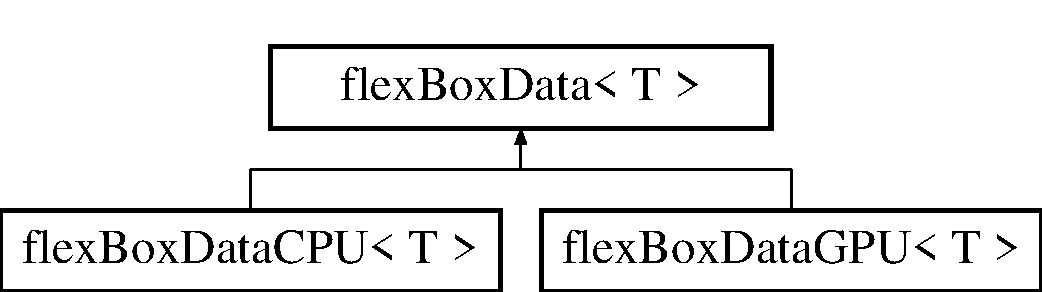
\includegraphics[height=2.000000cm]{classflex_box_data}
\end{center}
\end{figure}
\subsection*{Public Member Functions}
\begin{DoxyCompactItemize}
\item 
\mbox{\Hypertarget{classflex_box_data_a27e0928199d86a7e281308bf777aa8e2}\label{classflex_box_data_a27e0928199d86a7e281308bf777aa8e2}} 
void {\bfseries add\+Primal\+Var} (int number\+Of\+Elements)
\item 
\mbox{\Hypertarget{classflex_box_data_a9ca9476d38c912fd7576d94305a8e18c}\label{classflex_box_data_a9ca9476d38c912fd7576d94305a8e18c}} 
void {\bfseries add\+Dual\+Var} (int number\+Of\+Elements)
\item 
\mbox{\Hypertarget{classflex_box_data_a13623baeecd5c7a1b1eca93c2bbb8e0e}\label{classflex_box_data_a13623baeecd5c7a1b1eca93c2bbb8e0e}} 
int {\bfseries get\+Num\+Primal\+Vars} ()
\item 
\mbox{\Hypertarget{classflex_box_data_a4a9fb2a7ec29ad7a3bb4b7f041749d3a}\label{classflex_box_data_a4a9fb2a7ec29ad7a3bb4b7f041749d3a}} 
int {\bfseries get\+Num\+Dual\+Vars} ()
\item 
\mbox{\Hypertarget{classflex_box_data_a6cad656c27608f70f3fda907beb9a2ed}\label{classflex_box_data_a6cad656c27608f70f3fda907beb9a2ed}} 
virtual std\+::vector$<$ T $>$ {\bfseries get\+Primal} (int i)=0
\item 
\mbox{\Hypertarget{classflex_box_data_a3396e16e4c3a57279fd792fd84a76464}\label{classflex_box_data_a3396e16e4c3a57279fd792fd84a76464}} 
virtual std\+::vector$<$ T $>$ {\bfseries get\+Dual} (int i)=0
\item 
\mbox{\Hypertarget{classflex_box_data_a90cedf65f8a977d4a1944cce8df3d462}\label{classflex_box_data_a90cedf65f8a977d4a1944cce8df3d462}} 
virtual void {\bfseries set\+Primal} (int i, std\+::vector$<$ T $>$ input)=0
\item 
\mbox{\Hypertarget{classflex_box_data_a019d18a177433aefb77539ba48885153}\label{classflex_box_data_a019d18a177433aefb77539ba48885153}} 
virtual void {\bfseries set\+Dual} (int i, std\+::vector$<$ T $>$ input)=0
\end{DoxyCompactItemize}
\subsection*{Public Attributes}
\begin{DoxyCompactItemize}
\item 
\mbox{\Hypertarget{classflex_box_data_aa60ea99906fd551a207973e2ce9ffd15}\label{classflex_box_data_aa60ea99906fd551a207973e2ce9ffd15}} 
std\+::vector$<$ Tdata $>$ {\bfseries x}
\item 
\mbox{\Hypertarget{classflex_box_data_a5869c126458c3e86140a0147fd50a7de}\label{classflex_box_data_a5869c126458c3e86140a0147fd50a7de}} 
std\+::vector$<$ Tdata $>$ {\bfseries x\+Tmp}
\item 
\mbox{\Hypertarget{classflex_box_data_a888ab60110731e34e62913f96f595466}\label{classflex_box_data_a888ab60110731e34e62913f96f595466}} 
std\+::vector$<$ Tdata $>$ {\bfseries x\+Old}
\item 
\mbox{\Hypertarget{classflex_box_data_a007843962a1999a18b256c3f59b03609}\label{classflex_box_data_a007843962a1999a18b256c3f59b03609}} 
std\+::vector$<$ Tdata $>$ {\bfseries x\+Tilde}
\item 
\mbox{\Hypertarget{classflex_box_data_ae4f3b36c9d0f9d6e91156ef91f00ac59}\label{classflex_box_data_ae4f3b36c9d0f9d6e91156ef91f00ac59}} 
std\+::vector$<$ Tdata $>$ {\bfseries x\+Bar}
\item 
\mbox{\Hypertarget{classflex_box_data_a5ac559c209703d589baabc46c016d7f6}\label{classflex_box_data_a5ac559c209703d589baabc46c016d7f6}} 
std\+::vector$<$ Tdata $>$ {\bfseries x\+Error}
\item 
\mbox{\Hypertarget{classflex_box_data_ac8a0a62b2d5c5c6495caa45c196b603e}\label{classflex_box_data_ac8a0a62b2d5c5c6495caa45c196b603e}} 
std\+::vector$<$ Tdata $>$ {\bfseries y}
\item 
\mbox{\Hypertarget{classflex_box_data_a7269916b89fdaead632bb6309720cab8}\label{classflex_box_data_a7269916b89fdaead632bb6309720cab8}} 
std\+::vector$<$ Tdata $>$ {\bfseries y\+Tmp}
\item 
\mbox{\Hypertarget{classflex_box_data_ac09ee8f55031e7f8757d69774dcb0019}\label{classflex_box_data_ac09ee8f55031e7f8757d69774dcb0019}} 
std\+::vector$<$ Tdata $>$ {\bfseries y\+Old}
\item 
\mbox{\Hypertarget{classflex_box_data_afff3911c7c750bb8dd93561c42be3cbb}\label{classflex_box_data_afff3911c7c750bb8dd93561c42be3cbb}} 
std\+::vector$<$ Tdata $>$ {\bfseries y\+Tilde}
\item 
\mbox{\Hypertarget{classflex_box_data_a31bef4dbb95bb4e7cd5635a450787123}\label{classflex_box_data_a31bef4dbb95bb4e7cd5635a450787123}} 
std\+::vector$<$ Tdata $>$ {\bfseries y\+Error}
\item 
\mbox{\Hypertarget{classflex_box_data_a68cb4de5ab5e201bbe0c43a094af764a}\label{classflex_box_data_a68cb4de5ab5e201bbe0c43a094af764a}} 
std\+::vector$<$ Tdata $>$ {\bfseries tau\+Elt}
\item 
\mbox{\Hypertarget{classflex_box_data_ac258596d869c402b3b5e0b658d5d8016}\label{classflex_box_data_ac258596d869c402b3b5e0b658d5d8016}} 
std\+::vector$<$ Tdata $>$ {\bfseries sigma\+Elt}
\end{DoxyCompactItemize}


\subsection{Detailed Description}
\subsubsection*{template$<$typename T$>$\newline
class flex\+Box\+Data$<$ T $>$}

Flex\+Box data class. 

\hyperlink{classflex_box_data}{flex\+Box\+Data} is an internal abstract class for storing and maintaining data for the optimization algorithm used by the \hyperlink{classflex_box}{flex\+Box} main class. This class should not be used directly. 

The documentation for this class was generated from the following file\+:\begin{DoxyCompactItemize}
\item 
flex\+Box\+Data.\+h\end{DoxyCompactItemize}

\hypertarget{classflex_box_data_c_p_u}{}\section{flex\+Box\+Data\+C\+PU$<$ T $>$ Class Template Reference}
\label{classflex_box_data_c_p_u}\index{flex\+Box\+Data\+C\+P\+U$<$ T $>$@{flex\+Box\+Data\+C\+P\+U$<$ T $>$}}


Flex\+Box data class if using the non-\/\+C\+U\+DA version.  




{\ttfamily \#include $<$flex\+Box\+Data\+C\+P\+U.\+h$>$}

Inheritance diagram for flex\+Box\+Data\+C\+PU$<$ T $>$\+:\begin{figure}[H]
\begin{center}
\leavevmode
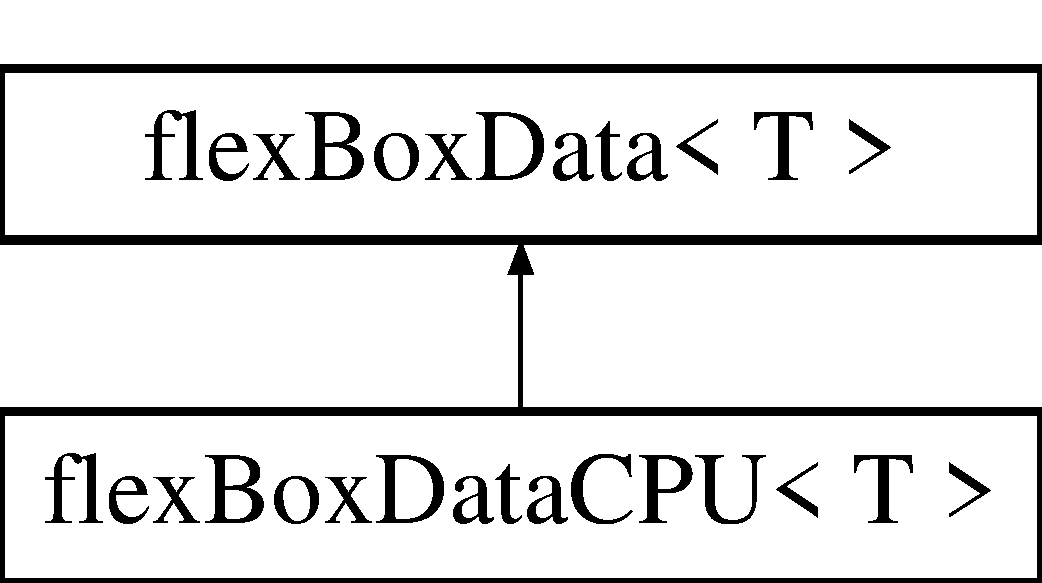
\includegraphics[height=2.000000cm]{classflex_box_data_c_p_u}
\end{center}
\end{figure}
\subsection*{Public Member Functions}
\begin{DoxyCompactItemize}
\item 
\mbox{\Hypertarget{classflex_box_data_c_p_u_a5465ee037c5120d2b1a4ef5bd53cc4d3}\label{classflex_box_data_c_p_u_a5465ee037c5120d2b1a4ef5bd53cc4d3}} 
std\+::vector$<$ T $>$ {\bfseries get\+Primal} (int i)
\item 
\mbox{\Hypertarget{classflex_box_data_c_p_u_a2edf696e874b8bed946c4594be519e21}\label{classflex_box_data_c_p_u_a2edf696e874b8bed946c4594be519e21}} 
std\+::vector$<$ T $>$ {\bfseries get\+Dual} (int i)
\item 
\mbox{\Hypertarget{classflex_box_data_c_p_u_ab2144460b3769bc396fbba51b9bd29ee}\label{classflex_box_data_c_p_u_ab2144460b3769bc396fbba51b9bd29ee}} 
void {\bfseries set\+Primal} (int i, std\+::vector$<$ T $>$ input)
\item 
\mbox{\Hypertarget{classflex_box_data_c_p_u_a9cdb107d16b65c6bcee32e4d44b0c5ef}\label{classflex_box_data_c_p_u_a9cdb107d16b65c6bcee32e4d44b0c5ef}} 
void {\bfseries set\+Dual} (int i, std\+::vector$<$ T $>$ input)
\end{DoxyCompactItemize}
\subsection*{Additional Inherited Members}


\subsection{Detailed Description}
\subsubsection*{template$<$class T$>$\newline
class flex\+Box\+Data\+C\+P\+U$<$ T $>$}

Flex\+Box data class if using the non-\/\+C\+U\+DA version. 

\hyperlink{classflex_box_data_c_p_u}{flex\+Box\+Data\+C\+PU} is an internal class for storing and maintaining data for the optimization algorithm if using the non-\/\+C\+U\+DA version. This class should not be used directly. 

The documentation for this class was generated from the following file\+:\begin{DoxyCompactItemize}
\item 
flex\+Box\+Data\+C\+P\+U.\+h\end{DoxyCompactItemize}

\hypertarget{classflex_box_data_g_p_u}{}\section{flex\+Box\+Data\+G\+PU$<$ T $>$ Class Template Reference}
\label{classflex_box_data_g_p_u}\index{flex\+Box\+Data\+G\+P\+U$<$ T $>$@{flex\+Box\+Data\+G\+P\+U$<$ T $>$}}


Flex\+Box data class if using the C\+U\+DA.  




{\ttfamily \#include $<$flex\+Box\+Data\+G\+P\+U.\+h$>$}

Inheritance diagram for flex\+Box\+Data\+G\+PU$<$ T $>$\+:\begin{figure}[H]
\begin{center}
\leavevmode
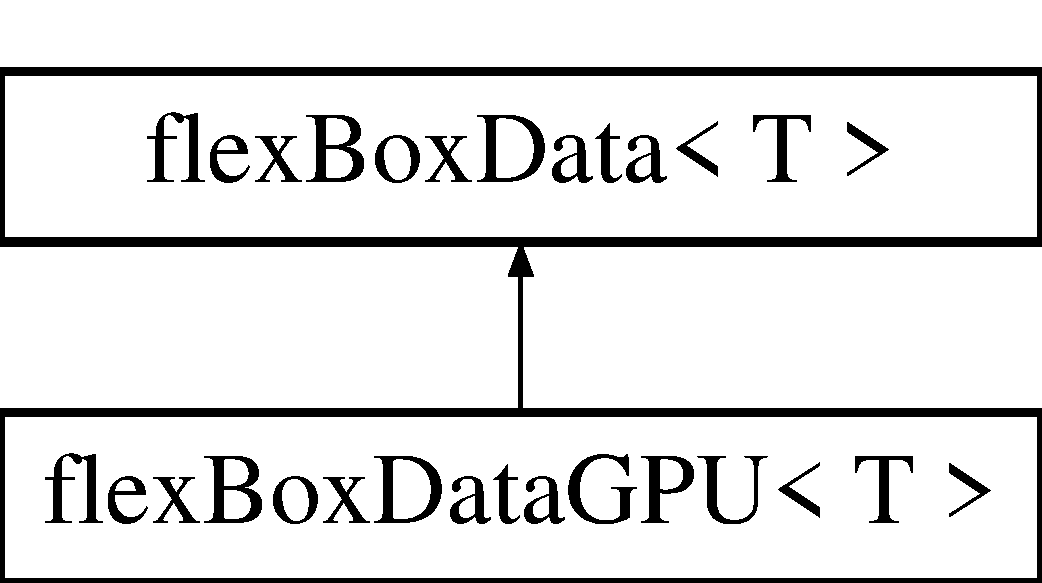
\includegraphics[height=2.000000cm]{classflex_box_data_g_p_u}
\end{center}
\end{figure}
\subsection*{Public Member Functions}
\begin{DoxyCompactItemize}
\item 
\mbox{\Hypertarget{classflex_box_data_g_p_u_a9c165e562583eea70011d70b815e5cfe}\label{classflex_box_data_g_p_u_a9c165e562583eea70011d70b815e5cfe}} 
std\+::vector$<$ T $>$ {\bfseries get\+Primal} (int i)
\item 
\mbox{\Hypertarget{classflex_box_data_g_p_u_a5f248d163e721a2a6f7cccea607a9f77}\label{classflex_box_data_g_p_u_a5f248d163e721a2a6f7cccea607a9f77}} 
std\+::vector$<$ T $>$ {\bfseries get\+Dual} (int i)
\item 
\mbox{\Hypertarget{classflex_box_data_g_p_u_a6543fc24f5c5a26b4a86e088a9b01572}\label{classflex_box_data_g_p_u_a6543fc24f5c5a26b4a86e088a9b01572}} 
void {\bfseries set\+Primal} (int i, std\+::vector$<$ T $>$ input)
\item 
\mbox{\Hypertarget{classflex_box_data_g_p_u_a5a110d8ef2b8c4d348cb73755b777288}\label{classflex_box_data_g_p_u_a5a110d8ef2b8c4d348cb73755b777288}} 
void {\bfseries set\+Dual} (int i, std\+::vector$<$ T $>$ input)
\end{DoxyCompactItemize}
\subsection*{Additional Inherited Members}


\subsection{Detailed Description}
\subsubsection*{template$<$class T$>$\newline
class flex\+Box\+Data\+G\+P\+U$<$ T $>$}

Flex\+Box data class if using the C\+U\+DA. 

\hyperlink{classflex_box_data_c_p_u}{flex\+Box\+Data\+C\+PU} is an internal class for storing and maintaining data for the optimization algorithm if using the C\+U\+DA version. This class should not be used directly. 

The documentation for this class was generated from the following file\+:\begin{DoxyCompactItemize}
\item 
flex\+Box\+Data\+G\+P\+U.\+h\end{DoxyCompactItemize}

\hypertarget{classflex_concat_operator}{}\section{flex\+Concat\+Operator$<$ T $>$ Class Template Reference}
\label{classflex_concat_operator}\index{flex\+Concat\+Operator$<$ T $>$@{flex\+Concat\+Operator$<$ T $>$}}


represents a concatenation operator  




{\ttfamily \#include $<$flex\+Concat\+Operator.\+h$>$}

Inheritance diagram for flex\+Concat\+Operator$<$ T $>$\+:\begin{figure}[H]
\begin{center}
\leavevmode
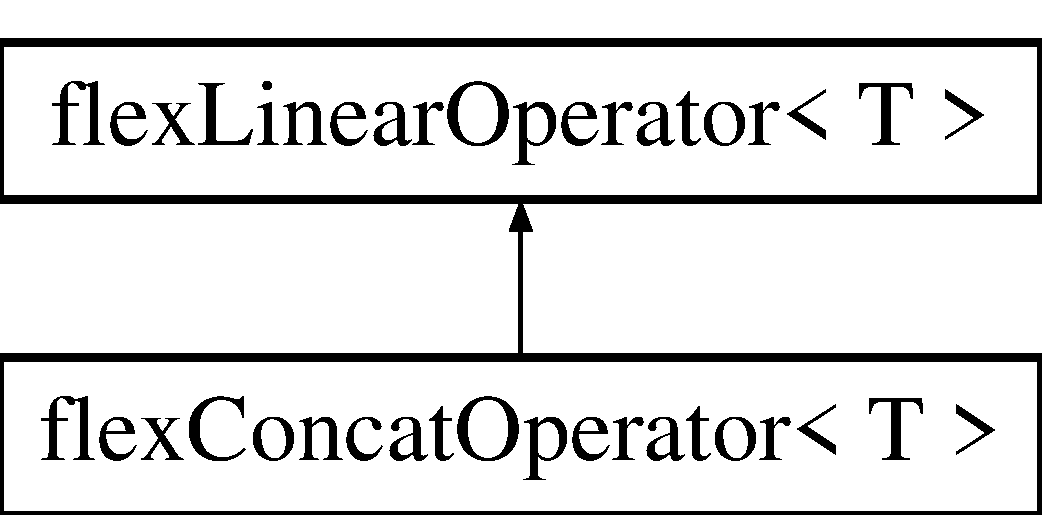
\includegraphics[height=2.000000cm]{classflex_concat_operator}
\end{center}
\end{figure}
\subsection*{Public Member Functions}
\begin{DoxyCompactItemize}
\item 
\hyperlink{classflex_concat_operator_aa0b80af6e02e39f68c5d2a07f5e7503d}{flex\+Concat\+Operator} (\hyperlink{classflex_linear_operator}{flex\+Linear\+Operator}$<$ T $>$ $\ast$aA, \hyperlink{classflex_linear_operator}{flex\+Linear\+Operator}$<$ T $>$ $\ast$aB, \hyperlink{tools_8h_ab8be8fa992a31c15058261e81ef8ba9d}{my\+Sign} aS, bool a\+Minus)
\begin{DoxyCompactList}\small\item\em initializes the concatenation operator \end{DoxyCompactList}\item 
\hyperlink{classflex_concat_operator}{flex\+Concat\+Operator}$<$ T $>$ $\ast$ \hyperlink{classflex_concat_operator_a8e554cb6edb47de0cf922cf51ec398b5}{copy} ()
\begin{DoxyCompactList}\small\item\em copies the linear operator \end{DoxyCompactList}\item 
void \hyperlink{classflex_concat_operator_af32c0fc8fc008a965d825dd0607ea388}{times} (bool transposed, const Tdata \&input, Tdata \&output)
\begin{DoxyCompactList}\small\item\em applies linear operator on vector \end{DoxyCompactList}\item 
void \hyperlink{classflex_concat_operator_a37962bd56dfb7853541e482f30a6ab23}{times\+Plus} (bool transposed, const Tdata \&input, Tdata \&output)
\begin{DoxyCompactList}\small\item\em applies linear operator on vector and adds its result to y \end{DoxyCompactList}\item 
void \hyperlink{classflex_concat_operator_a270c30ae4a8420729348eba8051ee322}{times\+Minus} (bool transposed, const Tdata \&input, Tdata \&output)
\begin{DoxyCompactList}\small\item\em applies linear operator on vector and substracts its result from y \end{DoxyCompactList}\item 
T \hyperlink{classflex_concat_operator_a39b7aa1797025fb022630a63358a4072}{get\+Max\+Row\+Sum\+Abs} (bool transposed)
\begin{DoxyCompactList}\small\item\em returns the maximum sum of absolute values per row used for preconditioning \end{DoxyCompactList}\item 
std\+::vector$<$ T $>$ \hyperlink{classflex_concat_operator_a6cae0c9545cf1afd8ac0ebc418fa3327}{get\+Abs\+Row\+Sum} (bool transposed)
\begin{DoxyCompactList}\small\item\em returns a vector of sum of absolute values per row used for preconditioning \end{DoxyCompactList}\item 
thrust\+::device\+\_\+vector$<$ T $>$ \hyperlink{classflex_concat_operator_a76e35865b16975bfcd6431879bda195b}{get\+Abs\+Row\+Sum\+C\+U\+DA} (bool transposed)
\begin{DoxyCompactList}\small\item\em same function as \hyperlink{classflex_concat_operator_a6cae0c9545cf1afd8ac0ebc418fa3327}{get\+Abs\+Row\+Sum()} but implemented in C\+U\+DA \end{DoxyCompactList}\end{DoxyCompactItemize}
\subsection*{Additional Inherited Members}


\subsection{Detailed Description}
\subsubsection*{template$<$typename T$>$\newline
class flex\+Concat\+Operator$<$ T $>$}

represents a concatenation operator 

\subsection{Constructor \& Destructor Documentation}
\mbox{\Hypertarget{classflex_concat_operator_aa0b80af6e02e39f68c5d2a07f5e7503d}\label{classflex_concat_operator_aa0b80af6e02e39f68c5d2a07f5e7503d}} 
\index{flex\+Concat\+Operator@{flex\+Concat\+Operator}!flex\+Concat\+Operator@{flex\+Concat\+Operator}}
\index{flex\+Concat\+Operator@{flex\+Concat\+Operator}!flex\+Concat\+Operator@{flex\+Concat\+Operator}}
\subsubsection{\texorpdfstring{flex\+Concat\+Operator()}{flexConcatOperator()}}
{\footnotesize\ttfamily template$<$typename T$>$ \\
\hyperlink{classflex_concat_operator}{flex\+Concat\+Operator}$<$ T $>$\+::\hyperlink{classflex_concat_operator}{flex\+Concat\+Operator} (\begin{DoxyParamCaption}\item[{\hyperlink{classflex_linear_operator}{flex\+Linear\+Operator}$<$ T $>$ $\ast$}]{aA,  }\item[{\hyperlink{classflex_linear_operator}{flex\+Linear\+Operator}$<$ T $>$ $\ast$}]{aB,  }\item[{\hyperlink{tools_8h_ab8be8fa992a31c15058261e81ef8ba9d}{my\+Sign}}]{aS,  }\item[{bool}]{a\+Minus }\end{DoxyParamCaption})\hspace{0.3cm}{\ttfamily [inline]}}



initializes the concatenation operator 


\begin{DoxyParams}{Parameters}
{\em aA} & left hand side operator \\
\hline
{\em aB} & right hand side operator \\
\hline
{\em aS} & type of concatenation. Possible values are P\+L\+US, S\+U\+B\+T\+R\+A\+CT and C\+O\+M\+P\+O\+SE. \\
\hline
{\em a\+Minus} & determines if operator is negated \\
\hline
\end{DoxyParams}
\begin{DoxySeeAlso}{See also}
\hyperlink{classflex_linear_operator_a7f986517e10aee21099ec7692b77905d}{is\+Minus} 
\end{DoxySeeAlso}


\subsection{Member Function Documentation}
\mbox{\Hypertarget{classflex_concat_operator_a8e554cb6edb47de0cf922cf51ec398b5}\label{classflex_concat_operator_a8e554cb6edb47de0cf922cf51ec398b5}} 
\index{flex\+Concat\+Operator@{flex\+Concat\+Operator}!copy@{copy}}
\index{copy@{copy}!flex\+Concat\+Operator@{flex\+Concat\+Operator}}
\subsubsection{\texorpdfstring{copy()}{copy()}}
{\footnotesize\ttfamily template$<$typename T$>$ \\
\hyperlink{classflex_concat_operator}{flex\+Concat\+Operator}$<$T$>$$\ast$ \hyperlink{classflex_concat_operator}{flex\+Concat\+Operator}$<$ T $>$\+::copy (\begin{DoxyParamCaption}{ }\end{DoxyParamCaption})\hspace{0.3cm}{\ttfamily [inline]}, {\ttfamily [virtual]}}



copies the linear operator 

\begin{DoxyReturn}{Returns}
copy of linear operator 
\end{DoxyReturn}


Implements \hyperlink{classflex_linear_operator_a7cc1425677cc30fcbd092ffd28d508c9}{flex\+Linear\+Operator$<$ T $>$}.

\mbox{\Hypertarget{classflex_concat_operator_a6cae0c9545cf1afd8ac0ebc418fa3327}\label{classflex_concat_operator_a6cae0c9545cf1afd8ac0ebc418fa3327}} 
\index{flex\+Concat\+Operator@{flex\+Concat\+Operator}!get\+Abs\+Row\+Sum@{get\+Abs\+Row\+Sum}}
\index{get\+Abs\+Row\+Sum@{get\+Abs\+Row\+Sum}!flex\+Concat\+Operator@{flex\+Concat\+Operator}}
\subsubsection{\texorpdfstring{get\+Abs\+Row\+Sum()}{getAbsRowSum()}}
{\footnotesize\ttfamily template$<$typename T$>$ \\
std\+::vector$<$T$>$ \hyperlink{classflex_concat_operator}{flex\+Concat\+Operator}$<$ T $>$\+::get\+Abs\+Row\+Sum (\begin{DoxyParamCaption}\item[{bool}]{transposed }\end{DoxyParamCaption})\hspace{0.3cm}{\ttfamily [inline]}, {\ttfamily [virtual]}}



returns a vector of sum of absolute values per row used for preconditioning 


\begin{DoxyParams}{Parameters}
{\em transposed} & is true if operator should be (temporarily) transposed before usage \\
\hline
\end{DoxyParams}
\begin{DoxyReturn}{Returns}
vector of sum of absolute values per row 
\end{DoxyReturn}


Implements \hyperlink{classflex_linear_operator_ad6caa7b09e6e3c401cadef61b8e2307e}{flex\+Linear\+Operator$<$ T $>$}.

\mbox{\Hypertarget{classflex_concat_operator_a76e35865b16975bfcd6431879bda195b}\label{classflex_concat_operator_a76e35865b16975bfcd6431879bda195b}} 
\index{flex\+Concat\+Operator@{flex\+Concat\+Operator}!get\+Abs\+Row\+Sum\+C\+U\+DA@{get\+Abs\+Row\+Sum\+C\+U\+DA}}
\index{get\+Abs\+Row\+Sum\+C\+U\+DA@{get\+Abs\+Row\+Sum\+C\+U\+DA}!flex\+Concat\+Operator@{flex\+Concat\+Operator}}
\subsubsection{\texorpdfstring{get\+Abs\+Row\+Sum\+C\+U\+D\+A()}{getAbsRowSumCUDA()}}
{\footnotesize\ttfamily template$<$typename T$>$ \\
thrust\+::device\+\_\+vector$<$T$>$ \hyperlink{classflex_concat_operator}{flex\+Concat\+Operator}$<$ T $>$\+::get\+Abs\+Row\+Sum\+C\+U\+DA (\begin{DoxyParamCaption}\item[{bool}]{transposed }\end{DoxyParamCaption})\hspace{0.3cm}{\ttfamily [inline]}, {\ttfamily [virtual]}}



same function as \hyperlink{classflex_concat_operator_a6cae0c9545cf1afd8ac0ebc418fa3327}{get\+Abs\+Row\+Sum()} but implemented in C\+U\+DA 


\begin{DoxyParams}{Parameters}
{\em transposed} & is true if operator should be (temporarily) transposed before usage \\
\hline
\end{DoxyParams}
\begin{DoxyReturn}{Returns}
vector of sum of absolute values per row 
\end{DoxyReturn}


Implements \hyperlink{classflex_linear_operator_a0a0a431d43f4f9d36cbee0d31ba5a29b}{flex\+Linear\+Operator$<$ T $>$}.

\mbox{\Hypertarget{classflex_concat_operator_a39b7aa1797025fb022630a63358a4072}\label{classflex_concat_operator_a39b7aa1797025fb022630a63358a4072}} 
\index{flex\+Concat\+Operator@{flex\+Concat\+Operator}!get\+Max\+Row\+Sum\+Abs@{get\+Max\+Row\+Sum\+Abs}}
\index{get\+Max\+Row\+Sum\+Abs@{get\+Max\+Row\+Sum\+Abs}!flex\+Concat\+Operator@{flex\+Concat\+Operator}}
\subsubsection{\texorpdfstring{get\+Max\+Row\+Sum\+Abs()}{getMaxRowSumAbs()}}
{\footnotesize\ttfamily template$<$typename T$>$ \\
T \hyperlink{classflex_concat_operator}{flex\+Concat\+Operator}$<$ T $>$\+::get\+Max\+Row\+Sum\+Abs (\begin{DoxyParamCaption}\item[{bool}]{transposed }\end{DoxyParamCaption})\hspace{0.3cm}{\ttfamily [inline]}, {\ttfamily [virtual]}}



returns the maximum sum of absolute values per row used for preconditioning 


\begin{DoxyParams}{Parameters}
{\em transposed} & is true if operator should be (temporarily) transposed before usage \\
\hline
\end{DoxyParams}
\begin{DoxyReturn}{Returns}
maximum sum of absolute values per row 
\end{DoxyReturn}


Implements \hyperlink{classflex_linear_operator_afcb74697385ccb7c8d29870d7034c12a}{flex\+Linear\+Operator$<$ T $>$}.

\mbox{\Hypertarget{classflex_concat_operator_af32c0fc8fc008a965d825dd0607ea388}\label{classflex_concat_operator_af32c0fc8fc008a965d825dd0607ea388}} 
\index{flex\+Concat\+Operator@{flex\+Concat\+Operator}!times@{times}}
\index{times@{times}!flex\+Concat\+Operator@{flex\+Concat\+Operator}}
\subsubsection{\texorpdfstring{times()}{times()}}
{\footnotesize\ttfamily template$<$typename T$>$ \\
void \hyperlink{classflex_concat_operator}{flex\+Concat\+Operator}$<$ T $>$\+::times (\begin{DoxyParamCaption}\item[{bool}]{transposed,  }\item[{const Tdata \&}]{input,  }\item[{Tdata \&}]{output }\end{DoxyParamCaption})\hspace{0.3cm}{\ttfamily [inline]}, {\ttfamily [virtual]}}



applies linear operator on vector 

equals $ y = Ax $ 
\begin{DoxyParams}{Parameters}
{\em transposed} & is true if operator should be (temporarily) transposed before usage \\
\hline
{\em input} & data to be processed \\
\hline
{\em output} & output data \\
\hline
\end{DoxyParams}


Implements \hyperlink{classflex_linear_operator_a883982edf3be857815d2095e53f76e75}{flex\+Linear\+Operator$<$ T $>$}.

\mbox{\Hypertarget{classflex_concat_operator_a270c30ae4a8420729348eba8051ee322}\label{classflex_concat_operator_a270c30ae4a8420729348eba8051ee322}} 
\index{flex\+Concat\+Operator@{flex\+Concat\+Operator}!times\+Minus@{times\+Minus}}
\index{times\+Minus@{times\+Minus}!flex\+Concat\+Operator@{flex\+Concat\+Operator}}
\subsubsection{\texorpdfstring{times\+Minus()}{timesMinus()}}
{\footnotesize\ttfamily template$<$typename T$>$ \\
void \hyperlink{classflex_concat_operator}{flex\+Concat\+Operator}$<$ T $>$\+::times\+Minus (\begin{DoxyParamCaption}\item[{bool}]{transposed,  }\item[{const Tdata \&}]{input,  }\item[{Tdata \&}]{output }\end{DoxyParamCaption})\hspace{0.3cm}{\ttfamily [inline]}, {\ttfamily [virtual]}}



applies linear operator on vector and substracts its result from y 

equals $ y = y - Ax $ 
\begin{DoxyParams}{Parameters}
{\em transposed} & is true if operator should be (temporarily) transposed before usage \\
\hline
{\em input} & data to be processed \\
\hline
{\em output} & output data \\
\hline
\end{DoxyParams}


Implements \hyperlink{classflex_linear_operator_a62708874e134a649c8445df333079c69}{flex\+Linear\+Operator$<$ T $>$}.

\mbox{\Hypertarget{classflex_concat_operator_a37962bd56dfb7853541e482f30a6ab23}\label{classflex_concat_operator_a37962bd56dfb7853541e482f30a6ab23}} 
\index{flex\+Concat\+Operator@{flex\+Concat\+Operator}!times\+Plus@{times\+Plus}}
\index{times\+Plus@{times\+Plus}!flex\+Concat\+Operator@{flex\+Concat\+Operator}}
\subsubsection{\texorpdfstring{times\+Plus()}{timesPlus()}}
{\footnotesize\ttfamily template$<$typename T$>$ \\
void \hyperlink{classflex_concat_operator}{flex\+Concat\+Operator}$<$ T $>$\+::times\+Plus (\begin{DoxyParamCaption}\item[{bool}]{transposed,  }\item[{const Tdata \&}]{input,  }\item[{Tdata \&}]{output }\end{DoxyParamCaption})\hspace{0.3cm}{\ttfamily [inline]}, {\ttfamily [virtual]}}



applies linear operator on vector and adds its result to y 

equals $ y = y + Ax $ 
\begin{DoxyParams}{Parameters}
{\em transposed} & is true if operator should be (temporarily) transposed before usage \\
\hline
{\em input} & data to be processed \\
\hline
{\em output} & output data \\
\hline
\end{DoxyParams}


Implements \hyperlink{classflex_linear_operator_a3f2978ad1c5eae8cd4ae16deb2337416}{flex\+Linear\+Operator$<$ T $>$}.



The documentation for this class was generated from the following file\+:\begin{DoxyCompactItemize}
\item 
flex\+Concat\+Operator.\+h\end{DoxyCompactItemize}

\hypertarget{classflex_diagonal_operator}{}\section{flex\+Diagonal\+Operator$<$ T $>$ Class Template Reference}
\label{classflex_diagonal_operator}\index{flex\+Diagonal\+Operator$<$ T $>$@{flex\+Diagonal\+Operator$<$ T $>$}}


represents a diagonal operator  




{\ttfamily \#include $<$flex\+Diagonal\+Operator.\+h$>$}

Inheritance diagram for flex\+Diagonal\+Operator$<$ T $>$\+:\begin{figure}[H]
\begin{center}
\leavevmode
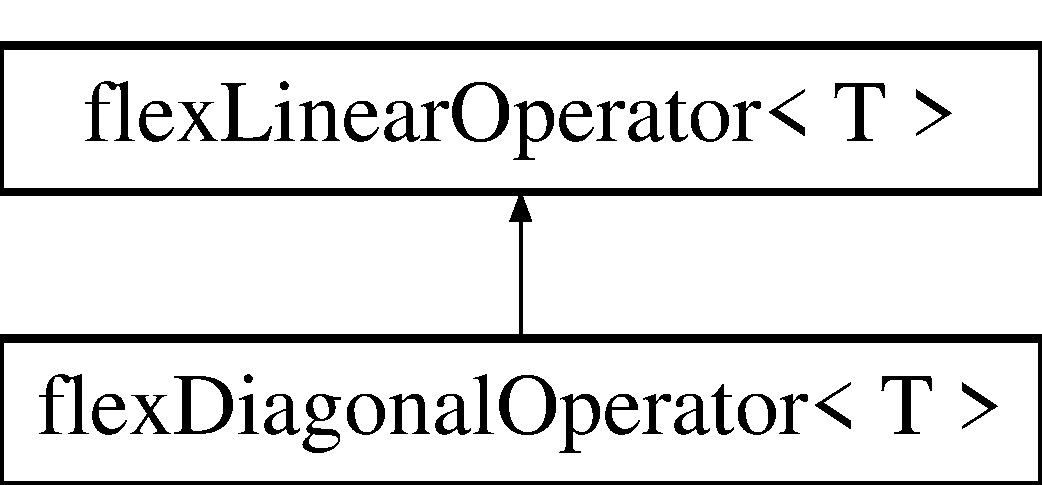
\includegraphics[height=2.000000cm]{classflex_diagonal_operator}
\end{center}
\end{figure}
\subsection*{Classes}
\begin{DoxyCompactItemize}
\item 
struct {\bfseries flex\+Diagonal\+Operator\+Functor}
\end{DoxyCompactItemize}
\subsection*{Public Member Functions}
\begin{DoxyCompactItemize}
\item 
\hyperlink{classflex_diagonal_operator_affc1bfd1944ccf07c179ae3d4855f7af}{flex\+Diagonal\+Operator} (std\+::vector$<$ T $>$ a\+Diagonal\+Elements, bool a\+Minus)
\begin{DoxyCompactList}\small\item\em initializes the concatenation operator for non-\/\+C\+U\+DA versions \end{DoxyCompactList}\item 
\hyperlink{classflex_diagonal_operator_a9e39335b75df3ac690aa3899f4a1a5e4}{flex\+Diagonal\+Operator} (Tdata a\+Diagonal\+Elements, bool a\+Minus)
\begin{DoxyCompactList}\small\item\em initializes the concatenation operator for C\+U\+DA versions \end{DoxyCompactList}\item 
\hyperlink{classflex_diagonal_operator}{flex\+Diagonal\+Operator}$<$ T $>$ $\ast$ \hyperlink{classflex_diagonal_operator_aeca7325de5eaface63363e9710034128}{copy} ()
\begin{DoxyCompactList}\small\item\em copies the linear operator \end{DoxyCompactList}\item 
void \hyperlink{classflex_diagonal_operator_a701d4741eb75d3e63fd47b936b46fb8c}{times} (bool transposed, const Tdata \&input, Tdata \&output)
\begin{DoxyCompactList}\small\item\em applies linear operator on vector \end{DoxyCompactList}\item 
void \hyperlink{classflex_diagonal_operator_ab8b9999592b97c6189f7f2c5d3bd47af}{times\+Plus} (bool transposed, const Tdata \&input, Tdata \&output)
\begin{DoxyCompactList}\small\item\em applies linear operator on vector and adds its result to y \end{DoxyCompactList}\item 
void \hyperlink{classflex_diagonal_operator_ac579880d56e9703a5fcb6cafbf9fe338}{times\+Minus} (bool transposed, const Tdata \&input, Tdata \&output)
\begin{DoxyCompactList}\small\item\em applies linear operator on vector and substracts its result from y \end{DoxyCompactList}\item 
std\+::vector$<$ T $>$ \hyperlink{classflex_diagonal_operator_ad53cb526b55141a1d0519a023572cf58}{get\+Abs\+Row\+Sum} (bool transposed)
\begin{DoxyCompactList}\small\item\em returns a vector of sum of absolute values per row used for preconditioning \end{DoxyCompactList}\item 
T \hyperlink{classflex_diagonal_operator_aa9c144ae23fbcbcdcd14cc779182896a}{get\+Max\+Row\+Sum\+Abs} (bool transposed)
\begin{DoxyCompactList}\small\item\em returns the maximum sum of absolute values per row used for preconditioning \end{DoxyCompactList}\item 
thrust\+::device\+\_\+vector$<$ T $>$ \hyperlink{classflex_diagonal_operator_a71cdb6ea6b8b7ceabaf538a180c8dcf4}{get\+Abs\+Row\+Sum\+C\+U\+DA} (bool transposed)
\begin{DoxyCompactList}\small\item\em same function as \hyperlink{classflex_diagonal_operator_ad53cb526b55141a1d0519a023572cf58}{get\+Abs\+Row\+Sum()} but implemented in C\+U\+DA \end{DoxyCompactList}\end{DoxyCompactItemize}
\subsection*{Additional Inherited Members}


\subsection{Detailed Description}
\subsubsection*{template$<$typename T$>$\newline
class flex\+Diagonal\+Operator$<$ T $>$}

represents a diagonal operator 

\subsection{Constructor \& Destructor Documentation}
\mbox{\Hypertarget{classflex_diagonal_operator_affc1bfd1944ccf07c179ae3d4855f7af}\label{classflex_diagonal_operator_affc1bfd1944ccf07c179ae3d4855f7af}} 
\index{flex\+Diagonal\+Operator@{flex\+Diagonal\+Operator}!flex\+Diagonal\+Operator@{flex\+Diagonal\+Operator}}
\index{flex\+Diagonal\+Operator@{flex\+Diagonal\+Operator}!flex\+Diagonal\+Operator@{flex\+Diagonal\+Operator}}
\subsubsection{\texorpdfstring{flex\+Diagonal\+Operator()}{flexDiagonalOperator()}\hspace{0.1cm}{\footnotesize\ttfamily [1/2]}}
{\footnotesize\ttfamily template$<$typename T$>$ \\
\hyperlink{classflex_diagonal_operator}{flex\+Diagonal\+Operator}$<$ T $>$\+::\hyperlink{classflex_diagonal_operator}{flex\+Diagonal\+Operator} (\begin{DoxyParamCaption}\item[{std\+::vector$<$ T $>$}]{a\+Diagonal\+Elements,  }\item[{bool}]{a\+Minus }\end{DoxyParamCaption})\hspace{0.3cm}{\ttfamily [inline]}}



initializes the concatenation operator for non-\/\+C\+U\+DA versions 


\begin{DoxyParams}{Parameters}
{\em a\+Diagonal\+Elements} & vector of diagonal Elements \\
\hline
{\em a\+Minus} & determines if operator is negated \\
\hline
\end{DoxyParams}
\begin{DoxySeeAlso}{See also}
\hyperlink{classflex_linear_operator_a7f986517e10aee21099ec7692b77905d}{is\+Minus} 
\end{DoxySeeAlso}
\mbox{\Hypertarget{classflex_diagonal_operator_a9e39335b75df3ac690aa3899f4a1a5e4}\label{classflex_diagonal_operator_a9e39335b75df3ac690aa3899f4a1a5e4}} 
\index{flex\+Diagonal\+Operator@{flex\+Diagonal\+Operator}!flex\+Diagonal\+Operator@{flex\+Diagonal\+Operator}}
\index{flex\+Diagonal\+Operator@{flex\+Diagonal\+Operator}!flex\+Diagonal\+Operator@{flex\+Diagonal\+Operator}}
\subsubsection{\texorpdfstring{flex\+Diagonal\+Operator()}{flexDiagonalOperator()}\hspace{0.1cm}{\footnotesize\ttfamily [2/2]}}
{\footnotesize\ttfamily template$<$typename T$>$ \\
\hyperlink{classflex_diagonal_operator}{flex\+Diagonal\+Operator}$<$ T $>$\+::\hyperlink{classflex_diagonal_operator}{flex\+Diagonal\+Operator} (\begin{DoxyParamCaption}\item[{Tdata}]{a\+Diagonal\+Elements,  }\item[{bool}]{a\+Minus }\end{DoxyParamCaption})\hspace{0.3cm}{\ttfamily [inline]}}



initializes the concatenation operator for C\+U\+DA versions 


\begin{DoxyParams}{Parameters}
{\em a\+Diagonal\+Elements} & vector of diagonal Elements where Tdata is of type thrust\+::device\+\_\+vector$<$\+T$>$ \\
\hline
{\em a\+Minus} & determines if operator is negated \\
\hline
\end{DoxyParams}
\begin{DoxySeeAlso}{See also}
\hyperlink{classflex_linear_operator_a7f986517e10aee21099ec7692b77905d}{is\+Minus} 
\end{DoxySeeAlso}


\subsection{Member Function Documentation}
\mbox{\Hypertarget{classflex_diagonal_operator_aeca7325de5eaface63363e9710034128}\label{classflex_diagonal_operator_aeca7325de5eaface63363e9710034128}} 
\index{flex\+Diagonal\+Operator@{flex\+Diagonal\+Operator}!copy@{copy}}
\index{copy@{copy}!flex\+Diagonal\+Operator@{flex\+Diagonal\+Operator}}
\subsubsection{\texorpdfstring{copy()}{copy()}}
{\footnotesize\ttfamily template$<$typename T$>$ \\
\hyperlink{classflex_diagonal_operator}{flex\+Diagonal\+Operator}$<$T$>$$\ast$ \hyperlink{classflex_diagonal_operator}{flex\+Diagonal\+Operator}$<$ T $>$\+::copy (\begin{DoxyParamCaption}{ }\end{DoxyParamCaption})\hspace{0.3cm}{\ttfamily [inline]}, {\ttfamily [virtual]}}



copies the linear operator 

\begin{DoxyReturn}{Returns}
copy of linear operator 
\end{DoxyReturn}


Implements \hyperlink{classflex_linear_operator_a7cc1425677cc30fcbd092ffd28d508c9}{flex\+Linear\+Operator$<$ T $>$}.

\mbox{\Hypertarget{classflex_diagonal_operator_ad53cb526b55141a1d0519a023572cf58}\label{classflex_diagonal_operator_ad53cb526b55141a1d0519a023572cf58}} 
\index{flex\+Diagonal\+Operator@{flex\+Diagonal\+Operator}!get\+Abs\+Row\+Sum@{get\+Abs\+Row\+Sum}}
\index{get\+Abs\+Row\+Sum@{get\+Abs\+Row\+Sum}!flex\+Diagonal\+Operator@{flex\+Diagonal\+Operator}}
\subsubsection{\texorpdfstring{get\+Abs\+Row\+Sum()}{getAbsRowSum()}}
{\footnotesize\ttfamily template$<$typename T$>$ \\
std\+::vector$<$T$>$ \hyperlink{classflex_diagonal_operator}{flex\+Diagonal\+Operator}$<$ T $>$\+::get\+Abs\+Row\+Sum (\begin{DoxyParamCaption}\item[{bool}]{transposed }\end{DoxyParamCaption})\hspace{0.3cm}{\ttfamily [inline]}, {\ttfamily [virtual]}}



returns a vector of sum of absolute values per row used for preconditioning 


\begin{DoxyParams}{Parameters}
{\em transposed} & is true if operator should be (temporarily) transposed before usage \\
\hline
\end{DoxyParams}
\begin{DoxyReturn}{Returns}
vector of sum of absolute values per row 
\end{DoxyReturn}


Implements \hyperlink{classflex_linear_operator_ad6caa7b09e6e3c401cadef61b8e2307e}{flex\+Linear\+Operator$<$ T $>$}.

\mbox{\Hypertarget{classflex_diagonal_operator_a71cdb6ea6b8b7ceabaf538a180c8dcf4}\label{classflex_diagonal_operator_a71cdb6ea6b8b7ceabaf538a180c8dcf4}} 
\index{flex\+Diagonal\+Operator@{flex\+Diagonal\+Operator}!get\+Abs\+Row\+Sum\+C\+U\+DA@{get\+Abs\+Row\+Sum\+C\+U\+DA}}
\index{get\+Abs\+Row\+Sum\+C\+U\+DA@{get\+Abs\+Row\+Sum\+C\+U\+DA}!flex\+Diagonal\+Operator@{flex\+Diagonal\+Operator}}
\subsubsection{\texorpdfstring{get\+Abs\+Row\+Sum\+C\+U\+D\+A()}{getAbsRowSumCUDA()}}
{\footnotesize\ttfamily template$<$typename T$>$ \\
thrust\+::device\+\_\+vector$<$T$>$ \hyperlink{classflex_diagonal_operator}{flex\+Diagonal\+Operator}$<$ T $>$\+::get\+Abs\+Row\+Sum\+C\+U\+DA (\begin{DoxyParamCaption}\item[{bool}]{transposed }\end{DoxyParamCaption})\hspace{0.3cm}{\ttfamily [inline]}, {\ttfamily [virtual]}}



same function as \hyperlink{classflex_diagonal_operator_ad53cb526b55141a1d0519a023572cf58}{get\+Abs\+Row\+Sum()} but implemented in C\+U\+DA 


\begin{DoxyParams}{Parameters}
{\em transposed} & is true if operator should be (temporarily) transposed before usage \\
\hline
\end{DoxyParams}
\begin{DoxyReturn}{Returns}
vector of sum of absolute values per row 
\end{DoxyReturn}


Implements \hyperlink{classflex_linear_operator_a0a0a431d43f4f9d36cbee0d31ba5a29b}{flex\+Linear\+Operator$<$ T $>$}.

\mbox{\Hypertarget{classflex_diagonal_operator_aa9c144ae23fbcbcdcd14cc779182896a}\label{classflex_diagonal_operator_aa9c144ae23fbcbcdcd14cc779182896a}} 
\index{flex\+Diagonal\+Operator@{flex\+Diagonal\+Operator}!get\+Max\+Row\+Sum\+Abs@{get\+Max\+Row\+Sum\+Abs}}
\index{get\+Max\+Row\+Sum\+Abs@{get\+Max\+Row\+Sum\+Abs}!flex\+Diagonal\+Operator@{flex\+Diagonal\+Operator}}
\subsubsection{\texorpdfstring{get\+Max\+Row\+Sum\+Abs()}{getMaxRowSumAbs()}}
{\footnotesize\ttfamily template$<$typename T$>$ \\
T \hyperlink{classflex_diagonal_operator}{flex\+Diagonal\+Operator}$<$ T $>$\+::get\+Max\+Row\+Sum\+Abs (\begin{DoxyParamCaption}\item[{bool}]{transposed }\end{DoxyParamCaption})\hspace{0.3cm}{\ttfamily [inline]}, {\ttfamily [virtual]}}



returns the maximum sum of absolute values per row used for preconditioning 


\begin{DoxyParams}{Parameters}
{\em transposed} & is true if operator should be (temporarily) transposed before usage \\
\hline
\end{DoxyParams}
\begin{DoxyReturn}{Returns}
maximum sum of absolute values per row 
\end{DoxyReturn}


Implements \hyperlink{classflex_linear_operator_afcb74697385ccb7c8d29870d7034c12a}{flex\+Linear\+Operator$<$ T $>$}.

\mbox{\Hypertarget{classflex_diagonal_operator_a701d4741eb75d3e63fd47b936b46fb8c}\label{classflex_diagonal_operator_a701d4741eb75d3e63fd47b936b46fb8c}} 
\index{flex\+Diagonal\+Operator@{flex\+Diagonal\+Operator}!times@{times}}
\index{times@{times}!flex\+Diagonal\+Operator@{flex\+Diagonal\+Operator}}
\subsubsection{\texorpdfstring{times()}{times()}}
{\footnotesize\ttfamily template$<$typename T$>$ \\
void \hyperlink{classflex_diagonal_operator}{flex\+Diagonal\+Operator}$<$ T $>$\+::times (\begin{DoxyParamCaption}\item[{bool}]{transposed,  }\item[{const Tdata \&}]{input,  }\item[{Tdata \&}]{output }\end{DoxyParamCaption})\hspace{0.3cm}{\ttfamily [inline]}, {\ttfamily [virtual]}}



applies linear operator on vector 

equals $ y = Ax $ 
\begin{DoxyParams}{Parameters}
{\em transposed} & is true if operator should be (temporarily) transposed before usage \\
\hline
{\em input} & data to be processed \\
\hline
{\em output} & output data \\
\hline
\end{DoxyParams}


Implements \hyperlink{classflex_linear_operator_a883982edf3be857815d2095e53f76e75}{flex\+Linear\+Operator$<$ T $>$}.

\mbox{\Hypertarget{classflex_diagonal_operator_ac579880d56e9703a5fcb6cafbf9fe338}\label{classflex_diagonal_operator_ac579880d56e9703a5fcb6cafbf9fe338}} 
\index{flex\+Diagonal\+Operator@{flex\+Diagonal\+Operator}!times\+Minus@{times\+Minus}}
\index{times\+Minus@{times\+Minus}!flex\+Diagonal\+Operator@{flex\+Diagonal\+Operator}}
\subsubsection{\texorpdfstring{times\+Minus()}{timesMinus()}}
{\footnotesize\ttfamily template$<$typename T$>$ \\
void \hyperlink{classflex_diagonal_operator}{flex\+Diagonal\+Operator}$<$ T $>$\+::times\+Minus (\begin{DoxyParamCaption}\item[{bool}]{transposed,  }\item[{const Tdata \&}]{input,  }\item[{Tdata \&}]{output }\end{DoxyParamCaption})\hspace{0.3cm}{\ttfamily [inline]}, {\ttfamily [virtual]}}



applies linear operator on vector and substracts its result from y 

equals $ y = y - Ax $ 
\begin{DoxyParams}{Parameters}
{\em transposed} & is true if operator should be (temporarily) transposed before usage \\
\hline
{\em input} & data to be processed \\
\hline
{\em output} & output data \\
\hline
\end{DoxyParams}


Implements \hyperlink{classflex_linear_operator_a62708874e134a649c8445df333079c69}{flex\+Linear\+Operator$<$ T $>$}.

\mbox{\Hypertarget{classflex_diagonal_operator_ab8b9999592b97c6189f7f2c5d3bd47af}\label{classflex_diagonal_operator_ab8b9999592b97c6189f7f2c5d3bd47af}} 
\index{flex\+Diagonal\+Operator@{flex\+Diagonal\+Operator}!times\+Plus@{times\+Plus}}
\index{times\+Plus@{times\+Plus}!flex\+Diagonal\+Operator@{flex\+Diagonal\+Operator}}
\subsubsection{\texorpdfstring{times\+Plus()}{timesPlus()}}
{\footnotesize\ttfamily template$<$typename T$>$ \\
void \hyperlink{classflex_diagonal_operator}{flex\+Diagonal\+Operator}$<$ T $>$\+::times\+Plus (\begin{DoxyParamCaption}\item[{bool}]{transposed,  }\item[{const Tdata \&}]{input,  }\item[{Tdata \&}]{output }\end{DoxyParamCaption})\hspace{0.3cm}{\ttfamily [inline]}, {\ttfamily [virtual]}}



applies linear operator on vector and adds its result to y 

equals $ y = y + Ax $ 
\begin{DoxyParams}{Parameters}
{\em transposed} & is true if operator should be (temporarily) transposed before usage \\
\hline
{\em input} & data to be processed \\
\hline
{\em output} & output data \\
\hline
\end{DoxyParams}


Implements \hyperlink{classflex_linear_operator_a3f2978ad1c5eae8cd4ae16deb2337416}{flex\+Linear\+Operator$<$ T $>$}.



The documentation for this class was generated from the following file\+:\begin{DoxyCompactItemize}
\item 
flex\+Diagonal\+Operator.\+h\end{DoxyCompactItemize}

\hypertarget{classflex_full_matrix}{}\section{flex\+Full\+Matrix$<$ T $>$ Class Template Reference}
\label{classflex_full_matrix}\index{flex\+Full\+Matrix$<$ T $>$@{flex\+Full\+Matrix$<$ T $>$}}


represents a full (non-\/\+C\+U\+DA) matrix  




{\ttfamily \#include $<$flex\+Full\+Matrix.\+h$>$}

Inheritance diagram for flex\+Full\+Matrix$<$ T $>$\+:\begin{figure}[H]
\begin{center}
\leavevmode
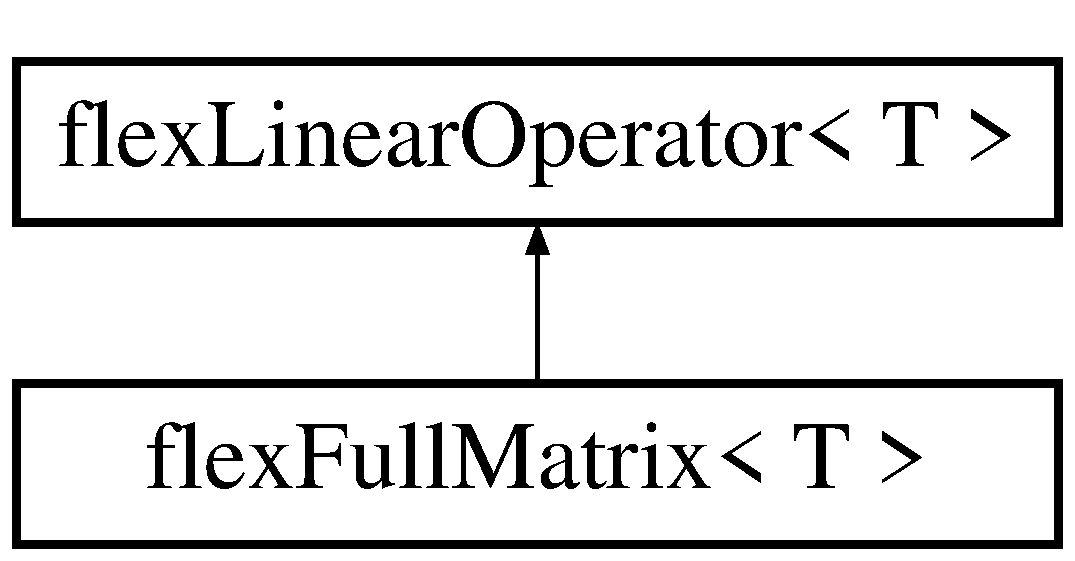
\includegraphics[height=2.000000cm]{classflex_full_matrix}
\end{center}
\end{figure}
\subsection*{Public Member Functions}
\begin{DoxyCompactItemize}
\item 
\mbox{\Hypertarget{classflex_full_matrix_a125feeded467ace162fc6b1002df6ef2}\label{classflex_full_matrix_a125feeded467ace162fc6b1002df6ef2}} 
\hyperlink{classflex_full_matrix_a125feeded467ace162fc6b1002df6ef2}{flex\+Full\+Matrix} ()
\begin{DoxyCompactList}\small\item\em initializes an empty matrix \end{DoxyCompactList}\item 
\hyperlink{classflex_full_matrix_a1523d991180fa00de2db44b10231987b}{flex\+Full\+Matrix} (int a\+Num\+Rows, int a\+Num\+Cols, bool a\+Minus)
\begin{DoxyCompactList}\small\item\em initializes a matrix \end{DoxyCompactList}\item 
\hyperlink{classflex_full_matrix}{flex\+Full\+Matrix}$<$ T $>$ $\ast$ \hyperlink{classflex_full_matrix_a849d2974a11456c6a23801f51838bc7b}{copy} ()
\begin{DoxyCompactList}\small\item\em copies the linear operator \end{DoxyCompactList}\item 
void \hyperlink{classflex_full_matrix_ad5c9cc8d3618cba2f96c963a6d180224}{times} (bool transposed, const Tdata \&input, Tdata \&output)
\begin{DoxyCompactList}\small\item\em applies linear operator on vector \end{DoxyCompactList}\item 
void \hyperlink{classflex_full_matrix_a5c5dc25704d934e28dd6944bbe4b3496}{times\+Plus} (bool transposed, const Tdata \&input, Tdata \&output)
\begin{DoxyCompactList}\small\item\em applies linear operator on vector and adds its result to y \end{DoxyCompactList}\item 
void \hyperlink{classflex_full_matrix_adf676d913b1409d6792fcd6cce144285}{times\+Minus} (bool transposed, const Tdata \&input, Tdata \&output)
\begin{DoxyCompactList}\small\item\em applies linear operator on vector and substracts its result from y \end{DoxyCompactList}\item 
\mbox{\Hypertarget{classflex_full_matrix_a5e800f6cfa4dce076db573506a4ef350}\label{classflex_full_matrix_a5e800f6cfa4dce076db573506a4ef350}} 
void {\bfseries insert\+Element} (int i, int j, T val)
\item 
\mbox{\Hypertarget{classflex_full_matrix_a9cbb6fb192b366be32bb53e3850830d6}\label{classflex_full_matrix_a9cbb6fb192b366be32bb53e3850830d6}} 
void {\bfseries insert\+Element} (int i, T val)
\item 
\mbox{\Hypertarget{classflex_full_matrix_a70f1a87d9e7cc34241fe0f46db0d3101}\label{classflex_full_matrix_a70f1a87d9e7cc34241fe0f46db0d3101}} 
int {\bfseries index2\+Dto\+Linear} (int i, int j)
\item 
T \hyperlink{classflex_full_matrix_a3ca8466b330c14b23689cb9f5507d40a}{get\+Max\+Row\+Sum\+Abs} (bool transposed)
\begin{DoxyCompactList}\small\item\em returns the maximum sum of absolute values per row used for preconditioning \end{DoxyCompactList}\item 
std\+::vector$<$ T $>$ \hyperlink{classflex_full_matrix_a911d6b2a452edb8233f56c1e5250855e}{get\+Abs\+Row\+Sum} (bool transposed)
\begin{DoxyCompactList}\small\item\em returns a vector of sum of absolute values per row used for preconditioning \end{DoxyCompactList}\item 
void \hyperlink{classflex_full_matrix_a0b9340f3b7a7559c56db7d1ce0d9d510}{print\+Row} (int i)
\begin{DoxyCompactList}\small\item\em prints requested row \end{DoxyCompactList}\item 
\mbox{\Hypertarget{classflex_full_matrix_ab61b7be5bc8b511f283be8a266c85833}\label{classflex_full_matrix_ab61b7be5bc8b511f283be8a266c85833}} 
void \hyperlink{classflex_full_matrix_ab61b7be5bc8b511f283be8a266c85833}{print\+Matrix} ()
\begin{DoxyCompactList}\small\item\em prints the whole matrix \end{DoxyCompactList}\item 
thrust\+::device\+\_\+vector$<$ T $>$ \hyperlink{classflex_full_matrix_af8ade69023e1c5140a82ad3583a8acb6}{get\+Abs\+Row\+Sum\+C\+U\+DA} (bool transposed)
\begin{DoxyCompactList}\small\item\em same function as \hyperlink{classflex_full_matrix_a911d6b2a452edb8233f56c1e5250855e}{get\+Abs\+Row\+Sum()} but implemented in C\+U\+DA \end{DoxyCompactList}\end{DoxyCompactItemize}
\subsection*{Additional Inherited Members}


\subsection{Detailed Description}
\subsubsection*{template$<$typename T$>$\newline
class flex\+Full\+Matrix$<$ T $>$}

represents a full (non-\/\+C\+U\+DA) matrix 

\subsection{Constructor \& Destructor Documentation}
\mbox{\Hypertarget{classflex_full_matrix_a1523d991180fa00de2db44b10231987b}\label{classflex_full_matrix_a1523d991180fa00de2db44b10231987b}} 
\index{flex\+Full\+Matrix@{flex\+Full\+Matrix}!flex\+Full\+Matrix@{flex\+Full\+Matrix}}
\index{flex\+Full\+Matrix@{flex\+Full\+Matrix}!flex\+Full\+Matrix@{flex\+Full\+Matrix}}
\subsubsection{\texorpdfstring{flex\+Full\+Matrix()}{flexFullMatrix()}}
{\footnotesize\ttfamily template$<$typename T$>$ \\
\hyperlink{classflex_full_matrix}{flex\+Full\+Matrix}$<$ T $>$\+::\hyperlink{classflex_full_matrix}{flex\+Full\+Matrix} (\begin{DoxyParamCaption}\item[{int}]{a\+Num\+Rows,  }\item[{int}]{a\+Num\+Cols,  }\item[{bool}]{a\+Minus }\end{DoxyParamCaption})\hspace{0.3cm}{\ttfamily [inline]}}



initializes a matrix 


\begin{DoxyParams}{Parameters}
{\em a\+Num\+Rows} & number of rows \\
\hline
{\em a\+Num\+Cols} & number of cols \\
\hline
{\em a\+Minus} & determines if operator is negated \\
\hline
\end{DoxyParams}
\begin{DoxySeeAlso}{See also}
\hyperlink{classflex_linear_operator_a7f986517e10aee21099ec7692b77905d}{is\+Minus} 
\end{DoxySeeAlso}


\subsection{Member Function Documentation}
\mbox{\Hypertarget{classflex_full_matrix_a849d2974a11456c6a23801f51838bc7b}\label{classflex_full_matrix_a849d2974a11456c6a23801f51838bc7b}} 
\index{flex\+Full\+Matrix@{flex\+Full\+Matrix}!copy@{copy}}
\index{copy@{copy}!flex\+Full\+Matrix@{flex\+Full\+Matrix}}
\subsubsection{\texorpdfstring{copy()}{copy()}}
{\footnotesize\ttfamily template$<$typename T$>$ \\
\hyperlink{classflex_full_matrix}{flex\+Full\+Matrix}$<$T$>$$\ast$ \hyperlink{classflex_full_matrix}{flex\+Full\+Matrix}$<$ T $>$\+::copy (\begin{DoxyParamCaption}{ }\end{DoxyParamCaption})\hspace{0.3cm}{\ttfamily [inline]}, {\ttfamily [virtual]}}



copies the linear operator 

\begin{DoxyReturn}{Returns}
copy of linear operator 
\end{DoxyReturn}


Implements \hyperlink{classflex_linear_operator_a7cc1425677cc30fcbd092ffd28d508c9}{flex\+Linear\+Operator$<$ T $>$}.

\mbox{\Hypertarget{classflex_full_matrix_a911d6b2a452edb8233f56c1e5250855e}\label{classflex_full_matrix_a911d6b2a452edb8233f56c1e5250855e}} 
\index{flex\+Full\+Matrix@{flex\+Full\+Matrix}!get\+Abs\+Row\+Sum@{get\+Abs\+Row\+Sum}}
\index{get\+Abs\+Row\+Sum@{get\+Abs\+Row\+Sum}!flex\+Full\+Matrix@{flex\+Full\+Matrix}}
\subsubsection{\texorpdfstring{get\+Abs\+Row\+Sum()}{getAbsRowSum()}}
{\footnotesize\ttfamily template$<$typename T$>$ \\
std\+::vector$<$T$>$ \hyperlink{classflex_full_matrix}{flex\+Full\+Matrix}$<$ T $>$\+::get\+Abs\+Row\+Sum (\begin{DoxyParamCaption}\item[{bool}]{transposed }\end{DoxyParamCaption})\hspace{0.3cm}{\ttfamily [inline]}, {\ttfamily [virtual]}}



returns a vector of sum of absolute values per row used for preconditioning 


\begin{DoxyParams}{Parameters}
{\em transposed} & is true if operator should be (temporarily) transposed before usage \\
\hline
\end{DoxyParams}
\begin{DoxyReturn}{Returns}
vector of sum of absolute values per row 
\end{DoxyReturn}


Implements \hyperlink{classflex_linear_operator_ad6caa7b09e6e3c401cadef61b8e2307e}{flex\+Linear\+Operator$<$ T $>$}.

\mbox{\Hypertarget{classflex_full_matrix_af8ade69023e1c5140a82ad3583a8acb6}\label{classflex_full_matrix_af8ade69023e1c5140a82ad3583a8acb6}} 
\index{flex\+Full\+Matrix@{flex\+Full\+Matrix}!get\+Abs\+Row\+Sum\+C\+U\+DA@{get\+Abs\+Row\+Sum\+C\+U\+DA}}
\index{get\+Abs\+Row\+Sum\+C\+U\+DA@{get\+Abs\+Row\+Sum\+C\+U\+DA}!flex\+Full\+Matrix@{flex\+Full\+Matrix}}
\subsubsection{\texorpdfstring{get\+Abs\+Row\+Sum\+C\+U\+D\+A()}{getAbsRowSumCUDA()}}
{\footnotesize\ttfamily template$<$typename T$>$ \\
thrust\+::device\+\_\+vector$<$T$>$ \hyperlink{classflex_full_matrix}{flex\+Full\+Matrix}$<$ T $>$\+::get\+Abs\+Row\+Sum\+C\+U\+DA (\begin{DoxyParamCaption}\item[{bool}]{transposed }\end{DoxyParamCaption})\hspace{0.3cm}{\ttfamily [inline]}, {\ttfamily [virtual]}}



same function as \hyperlink{classflex_full_matrix_a911d6b2a452edb8233f56c1e5250855e}{get\+Abs\+Row\+Sum()} but implemented in C\+U\+DA 


\begin{DoxyParams}{Parameters}
{\em transposed} & is true if operator should be (temporarily) transposed before usage \\
\hline
\end{DoxyParams}
\begin{DoxyReturn}{Returns}
vector of sum of absolute values per row 
\end{DoxyReturn}


Implements \hyperlink{classflex_linear_operator_a0a0a431d43f4f9d36cbee0d31ba5a29b}{flex\+Linear\+Operator$<$ T $>$}.

\mbox{\Hypertarget{classflex_full_matrix_a3ca8466b330c14b23689cb9f5507d40a}\label{classflex_full_matrix_a3ca8466b330c14b23689cb9f5507d40a}} 
\index{flex\+Full\+Matrix@{flex\+Full\+Matrix}!get\+Max\+Row\+Sum\+Abs@{get\+Max\+Row\+Sum\+Abs}}
\index{get\+Max\+Row\+Sum\+Abs@{get\+Max\+Row\+Sum\+Abs}!flex\+Full\+Matrix@{flex\+Full\+Matrix}}
\subsubsection{\texorpdfstring{get\+Max\+Row\+Sum\+Abs()}{getMaxRowSumAbs()}}
{\footnotesize\ttfamily template$<$typename T$>$ \\
T \hyperlink{classflex_full_matrix}{flex\+Full\+Matrix}$<$ T $>$\+::get\+Max\+Row\+Sum\+Abs (\begin{DoxyParamCaption}\item[{bool}]{transposed }\end{DoxyParamCaption})\hspace{0.3cm}{\ttfamily [inline]}, {\ttfamily [virtual]}}



returns the maximum sum of absolute values per row used for preconditioning 


\begin{DoxyParams}{Parameters}
{\em transposed} & is true if operator should be (temporarily) transposed before usage \\
\hline
\end{DoxyParams}
\begin{DoxyReturn}{Returns}
maximum sum of absolute values per row 
\end{DoxyReturn}


Implements \hyperlink{classflex_linear_operator_afcb74697385ccb7c8d29870d7034c12a}{flex\+Linear\+Operator$<$ T $>$}.

\mbox{\Hypertarget{classflex_full_matrix_a0b9340f3b7a7559c56db7d1ce0d9d510}\label{classflex_full_matrix_a0b9340f3b7a7559c56db7d1ce0d9d510}} 
\index{flex\+Full\+Matrix@{flex\+Full\+Matrix}!print\+Row@{print\+Row}}
\index{print\+Row@{print\+Row}!flex\+Full\+Matrix@{flex\+Full\+Matrix}}
\subsubsection{\texorpdfstring{print\+Row()}{printRow()}}
{\footnotesize\ttfamily template$<$typename T$>$ \\
void \hyperlink{classflex_full_matrix}{flex\+Full\+Matrix}$<$ T $>$\+::print\+Row (\begin{DoxyParamCaption}\item[{int}]{i }\end{DoxyParamCaption})\hspace{0.3cm}{\ttfamily [inline]}}



prints requested row 


\begin{DoxyParams}{Parameters}
{\em i} & row to be printed \\
\hline
\end{DoxyParams}
\mbox{\Hypertarget{classflex_full_matrix_ad5c9cc8d3618cba2f96c963a6d180224}\label{classflex_full_matrix_ad5c9cc8d3618cba2f96c963a6d180224}} 
\index{flex\+Full\+Matrix@{flex\+Full\+Matrix}!times@{times}}
\index{times@{times}!flex\+Full\+Matrix@{flex\+Full\+Matrix}}
\subsubsection{\texorpdfstring{times()}{times()}}
{\footnotesize\ttfamily template$<$typename T$>$ \\
void \hyperlink{classflex_full_matrix}{flex\+Full\+Matrix}$<$ T $>$\+::times (\begin{DoxyParamCaption}\item[{bool}]{transposed,  }\item[{const Tdata \&}]{input,  }\item[{Tdata \&}]{output }\end{DoxyParamCaption})\hspace{0.3cm}{\ttfamily [inline]}, {\ttfamily [virtual]}}



applies linear operator on vector 

equals $ y = Ax $ 
\begin{DoxyParams}{Parameters}
{\em transposed} & is true if operator should be (temporarily) transposed before usage \\
\hline
{\em input} & data to be processed \\
\hline
{\em output} & output data \\
\hline
\end{DoxyParams}


Implements \hyperlink{classflex_linear_operator_a883982edf3be857815d2095e53f76e75}{flex\+Linear\+Operator$<$ T $>$}.

\mbox{\Hypertarget{classflex_full_matrix_adf676d913b1409d6792fcd6cce144285}\label{classflex_full_matrix_adf676d913b1409d6792fcd6cce144285}} 
\index{flex\+Full\+Matrix@{flex\+Full\+Matrix}!times\+Minus@{times\+Minus}}
\index{times\+Minus@{times\+Minus}!flex\+Full\+Matrix@{flex\+Full\+Matrix}}
\subsubsection{\texorpdfstring{times\+Minus()}{timesMinus()}}
{\footnotesize\ttfamily template$<$typename T$>$ \\
void \hyperlink{classflex_full_matrix}{flex\+Full\+Matrix}$<$ T $>$\+::times\+Minus (\begin{DoxyParamCaption}\item[{bool}]{transposed,  }\item[{const Tdata \&}]{input,  }\item[{Tdata \&}]{output }\end{DoxyParamCaption})\hspace{0.3cm}{\ttfamily [inline]}, {\ttfamily [virtual]}}



applies linear operator on vector and substracts its result from y 

equals $ y = y - Ax $ 
\begin{DoxyParams}{Parameters}
{\em transposed} & is true if operator should be (temporarily) transposed before usage \\
\hline
{\em input} & data to be processed \\
\hline
{\em output} & output data \\
\hline
\end{DoxyParams}


Implements \hyperlink{classflex_linear_operator_a62708874e134a649c8445df333079c69}{flex\+Linear\+Operator$<$ T $>$}.

\mbox{\Hypertarget{classflex_full_matrix_a5c5dc25704d934e28dd6944bbe4b3496}\label{classflex_full_matrix_a5c5dc25704d934e28dd6944bbe4b3496}} 
\index{flex\+Full\+Matrix@{flex\+Full\+Matrix}!times\+Plus@{times\+Plus}}
\index{times\+Plus@{times\+Plus}!flex\+Full\+Matrix@{flex\+Full\+Matrix}}
\subsubsection{\texorpdfstring{times\+Plus()}{timesPlus()}}
{\footnotesize\ttfamily template$<$typename T$>$ \\
void \hyperlink{classflex_full_matrix}{flex\+Full\+Matrix}$<$ T $>$\+::times\+Plus (\begin{DoxyParamCaption}\item[{bool}]{transposed,  }\item[{const Tdata \&}]{input,  }\item[{Tdata \&}]{output }\end{DoxyParamCaption})\hspace{0.3cm}{\ttfamily [inline]}, {\ttfamily [virtual]}}



applies linear operator on vector and adds its result to y 

equals $ y = y + Ax $ 
\begin{DoxyParams}{Parameters}
{\em transposed} & is true if operator should be (temporarily) transposed before usage \\
\hline
{\em input} & data to be processed \\
\hline
{\em output} & output data \\
\hline
\end{DoxyParams}


Implements \hyperlink{classflex_linear_operator_a3f2978ad1c5eae8cd4ae16deb2337416}{flex\+Linear\+Operator$<$ T $>$}.



The documentation for this class was generated from the following file\+:\begin{DoxyCompactItemize}
\item 
flex\+Full\+Matrix.\+h\end{DoxyCompactItemize}

\hypertarget{classflex_gradient_operator}{}\section{flex\+Gradient\+Operator$<$ T $>$ Class Template Reference}
\label{classflex_gradient_operator}\index{flex\+Gradient\+Operator$<$ T $>$@{flex\+Gradient\+Operator$<$ T $>$}}


represents a gradient operator  




{\ttfamily \#include $<$flex\+Gradient\+Operator.\+h$>$}

Inheritance diagram for flex\+Gradient\+Operator$<$ T $>$\+:\begin{figure}[H]
\begin{center}
\leavevmode
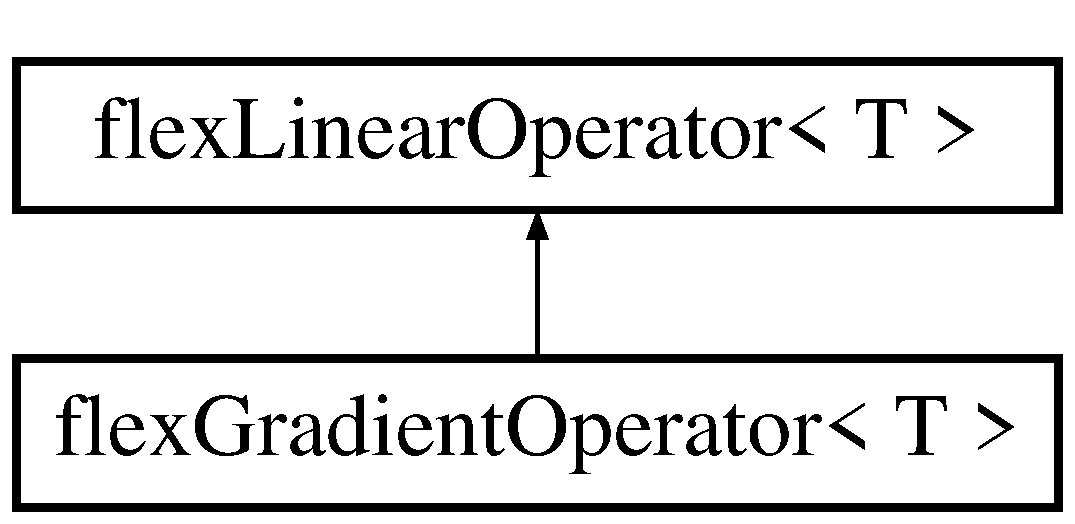
\includegraphics[height=2.000000cm]{classflex_gradient_operator}
\end{center}
\end{figure}
\subsection*{Public Member Functions}
\begin{DoxyCompactItemize}
\item 
\hyperlink{classflex_gradient_operator_aa83ae15b09ba2195951d8df803f08705}{flex\+Gradient\+Operator} (std\+::vector$<$ int $>$ A\+Input\+Dimension, int a\+Grad\+Direction, \hyperlink{tools_8h_a40b3c158323c8bcb80e2095f3473213c}{gradient\+Type} a\+Type, bool a\+Minus)
\begin{DoxyCompactList}\small\item\em initializes the gradient operator \end{DoxyCompactList}\item 
\hyperlink{classflex_gradient_operator}{flex\+Gradient\+Operator}$<$ T $>$ $\ast$ \hyperlink{classflex_gradient_operator_a4b1480051ac7763da809c509685316d2}{copy} ()
\begin{DoxyCompactList}\small\item\em copies the linear operator \end{DoxyCompactList}\item 
\mbox{\Hypertarget{classflex_gradient_operator_a1e71bbd56e480f5444ff6e32b0002040}\label{classflex_gradient_operator_a1e71bbd56e480f5444ff6e32b0002040}} 
void {\bfseries update\+Value} (T $\ast$ptr, \hyperlink{tools_8h_ab8be8fa992a31c15058261e81ef8ba9d}{my\+Sign} s, T value)
\item 
\mbox{\Hypertarget{classflex_gradient_operator_ad468dc07bc6e302bf8931d45ba8efaa6}\label{classflex_gradient_operator_ad468dc07bc6e302bf8931d45ba8efaa6}} 
void {\bfseries dxp3d} (const Tdata \&input, Tdata \&output, \hyperlink{tools_8h_ab8be8fa992a31c15058261e81ef8ba9d}{my\+Sign} s)
\item 
\mbox{\Hypertarget{classflex_gradient_operator_a7435c2408c7be34206a4662da37fe058}\label{classflex_gradient_operator_a7435c2408c7be34206a4662da37fe058}} 
void {\bfseries dyp3d} (const Tdata \&input, Tdata \&output, \hyperlink{tools_8h_ab8be8fa992a31c15058261e81ef8ba9d}{my\+Sign} s)
\item 
\mbox{\Hypertarget{classflex_gradient_operator_a5eefd707f1f71f20c2abbe7160d660b3}\label{classflex_gradient_operator_a5eefd707f1f71f20c2abbe7160d660b3}} 
void {\bfseries dzp3d} (const Tdata \&input, Tdata \&output, \hyperlink{tools_8h_ab8be8fa992a31c15058261e81ef8ba9d}{my\+Sign} s)
\item 
\mbox{\Hypertarget{classflex_gradient_operator_a6de07d9888e203f7eaa0f630f3d57c18}\label{classflex_gradient_operator_a6de07d9888e203f7eaa0f630f3d57c18}} 
void {\bfseries dxp3d\+Transposed} (const Tdata \&input, Tdata \&output, \hyperlink{tools_8h_ab8be8fa992a31c15058261e81ef8ba9d}{my\+Sign} s)
\item 
\mbox{\Hypertarget{classflex_gradient_operator_a0c5efa1ceda6ee9e0ad626150557fc4b}\label{classflex_gradient_operator_a0c5efa1ceda6ee9e0ad626150557fc4b}} 
void {\bfseries dyp3d\+Transposed} (const Tdata \&input, Tdata \&output, \hyperlink{tools_8h_ab8be8fa992a31c15058261e81ef8ba9d}{my\+Sign} s)
\item 
\mbox{\Hypertarget{classflex_gradient_operator_a1a00cc0370e270af955cac8174d30285}\label{classflex_gradient_operator_a1a00cc0370e270af955cac8174d30285}} 
void {\bfseries dzp3d\+Transposed} (const Tdata \&input, Tdata \&output, \hyperlink{tools_8h_ab8be8fa992a31c15058261e81ef8ba9d}{my\+Sign} s)
\item 
\mbox{\Hypertarget{classflex_gradient_operator_a89682c6d26bb9a8aa7ea1fc57a734009}\label{classflex_gradient_operator_a89682c6d26bb9a8aa7ea1fc57a734009}} 
void {\bfseries dxp2d} (const Tdata \&input, Tdata \&output, \hyperlink{tools_8h_ab8be8fa992a31c15058261e81ef8ba9d}{my\+Sign} s)
\item 
\mbox{\Hypertarget{classflex_gradient_operator_a3e2d15e37779ce04a9f082dfd127f545}\label{classflex_gradient_operator_a3e2d15e37779ce04a9f082dfd127f545}} 
void {\bfseries dyp2d} (const Tdata \&input, Tdata \&output, \hyperlink{tools_8h_ab8be8fa992a31c15058261e81ef8ba9d}{my\+Sign} s)
\item 
\mbox{\Hypertarget{classflex_gradient_operator_ab2266e66d3afe4d6c3752e145d07444c}\label{classflex_gradient_operator_ab2266e66d3afe4d6c3752e145d07444c}} 
void {\bfseries dxp2d\+Transposed} (const Tdata \&input, Tdata \&output, \hyperlink{tools_8h_ab8be8fa992a31c15058261e81ef8ba9d}{my\+Sign} s)
\item 
\mbox{\Hypertarget{classflex_gradient_operator_a202c728fbd7909e2926d78f35d2dedfc}\label{classflex_gradient_operator_a202c728fbd7909e2926d78f35d2dedfc}} 
void {\bfseries dyp2d\+Transposed} (const Tdata \&input, Tdata \&output, \hyperlink{tools_8h_ab8be8fa992a31c15058261e81ef8ba9d}{my\+Sign} s)
\item 
\mbox{\Hypertarget{classflex_gradient_operator_ae006fcafaae94e9b905fa4dba5296e80}\label{classflex_gradient_operator_ae006fcafaae94e9b905fa4dba5296e80}} 
void {\bfseries do\+Times\+C\+PU} (bool transposed, const Tdata \&input, Tdata \&output, \hyperlink{tools_8h_ab8be8fa992a31c15058261e81ef8ba9d}{my\+Sign} s)
\item 
\mbox{\Hypertarget{classflex_gradient_operator_a45cd508b73224f5339bc467e55876b80}\label{classflex_gradient_operator_a45cd508b73224f5339bc467e55876b80}} 
void {\bfseries do\+Times\+C\+U\+DA} (bool transposed, const Tdata \&input, Tdata \&output, \hyperlink{tools_8h_ab8be8fa992a31c15058261e81ef8ba9d}{my\+Sign} s)
\item 
\mbox{\Hypertarget{classflex_gradient_operator_a75d702d6d1cc0fce5d5c45c2294aba59}\label{classflex_gradient_operator_a75d702d6d1cc0fce5d5c45c2294aba59}} 
void {\bfseries do\+Times} (bool transposed, const Tdata \&input, Tdata \&output, \hyperlink{tools_8h_ab8be8fa992a31c15058261e81ef8ba9d}{my\+Sign} s)
\item 
void \hyperlink{classflex_gradient_operator_a1b6c9b788e6d5a62ba008811f287f8e5}{times\+Plus} (bool transposed, const Tdata \&input, Tdata \&output)
\begin{DoxyCompactList}\small\item\em applies linear operator on vector and adds its result to y \end{DoxyCompactList}\item 
void \hyperlink{classflex_gradient_operator_a287f5efd41aa14ee61aee87dfed08b88}{times\+Minus} (bool transposed, const Tdata \&input, Tdata \&output)
\begin{DoxyCompactList}\small\item\em applies linear operator on vector and substracts its result from y \end{DoxyCompactList}\item 
void \hyperlink{classflex_gradient_operator_aae5e807f99c3634c52b79f08d72fa7a2}{times} (bool transposed, const Tdata \&input, Tdata \&output)
\begin{DoxyCompactList}\small\item\em applies linear operator on vector \end{DoxyCompactList}\item 
T \hyperlink{classflex_gradient_operator_a6acb61ea8abf404d63be4574976391bb}{get\+Max\+Row\+Sum\+Abs} (bool transposed)
\begin{DoxyCompactList}\small\item\em returns the maximum sum of absolute values per row used for preconditioning \end{DoxyCompactList}\item 
std\+::vector$<$ T $>$ \hyperlink{classflex_gradient_operator_a04950a1e57f7587b95824bfd82b35738}{get\+Abs\+Row\+Sum} (bool transposed)
\begin{DoxyCompactList}\small\item\em returns a vector of sum of absolute values per row used for preconditioning \end{DoxyCompactList}\item 
\mbox{\Hypertarget{classflex_gradient_operator_add0b4fb2eed25bc6386abd8219e516ff}\label{classflex_gradient_operator_add0b4fb2eed25bc6386abd8219e516ff}} 
int {\bfseries index3\+Dto\+Linear} (int i, int j, int k)
\item 
\mbox{\Hypertarget{classflex_gradient_operator_a3dcfa503fb5b55b1c9629399bfb79c0d}\label{classflex_gradient_operator_a3dcfa503fb5b55b1c9629399bfb79c0d}} 
int {\bfseries index2\+Dto\+Linear} (int i, int j)
\item 
thrust\+::device\+\_\+vector$<$ T $>$ \hyperlink{classflex_gradient_operator_ac5cf151db87946ac0f1864344db260d5}{get\+Abs\+Row\+Sum\+C\+U\+DA} (bool transposed)
\begin{DoxyCompactList}\small\item\em same function as \hyperlink{classflex_gradient_operator_a04950a1e57f7587b95824bfd82b35738}{get\+Abs\+Row\+Sum()} but implemented in C\+U\+DA \end{DoxyCompactList}\end{DoxyCompactItemize}
\subsection*{Additional Inherited Members}


\subsection{Detailed Description}
\subsubsection*{template$<$typename T$>$\newline
class flex\+Gradient\+Operator$<$ T $>$}

represents a gradient operator 

\subsection{Constructor \& Destructor Documentation}
\mbox{\Hypertarget{classflex_gradient_operator_aa83ae15b09ba2195951d8df803f08705}\label{classflex_gradient_operator_aa83ae15b09ba2195951d8df803f08705}} 
\index{flex\+Gradient\+Operator@{flex\+Gradient\+Operator}!flex\+Gradient\+Operator@{flex\+Gradient\+Operator}}
\index{flex\+Gradient\+Operator@{flex\+Gradient\+Operator}!flex\+Gradient\+Operator@{flex\+Gradient\+Operator}}
\subsubsection{\texorpdfstring{flex\+Gradient\+Operator()}{flexGradientOperator()}}
{\footnotesize\ttfamily template$<$typename T $>$ \\
\hyperlink{classflex_gradient_operator}{flex\+Gradient\+Operator}$<$ T $>$\+::\hyperlink{classflex_gradient_operator}{flex\+Gradient\+Operator} (\begin{DoxyParamCaption}\item[{std\+::vector$<$ int $>$}]{A\+Input\+Dimension,  }\item[{int}]{a\+Grad\+Direction,  }\item[{\hyperlink{tools_8h_a40b3c158323c8bcb80e2095f3473213c}{gradient\+Type}}]{a\+Type,  }\item[{bool}]{a\+Minus }\end{DoxyParamCaption})\hspace{0.3cm}{\ttfamily [inline]}}



initializes the gradient operator 


\begin{DoxyParams}{Parameters}
{\em A\+Input\+Dimension} & vector of dimensions \\
\hline
{\em a\+Grad\+Direction} & direction of gradient. 0 for first dimension and so on. \\
\hline
{\em a\+Type} & type of gradient. Possible values are forward, backward and central. \\
\hline
{\em a\+Minus} & determines if operator is negated \\
\hline
\end{DoxyParams}
\begin{DoxySeeAlso}{See also}
\hyperlink{classflex_linear_operator_a7f986517e10aee21099ec7692b77905d}{is\+Minus} 
\end{DoxySeeAlso}


\subsection{Member Function Documentation}
\mbox{\Hypertarget{classflex_gradient_operator_a4b1480051ac7763da809c509685316d2}\label{classflex_gradient_operator_a4b1480051ac7763da809c509685316d2}} 
\index{flex\+Gradient\+Operator@{flex\+Gradient\+Operator}!copy@{copy}}
\index{copy@{copy}!flex\+Gradient\+Operator@{flex\+Gradient\+Operator}}
\subsubsection{\texorpdfstring{copy()}{copy()}}
{\footnotesize\ttfamily template$<$typename T $>$ \\
\hyperlink{classflex_gradient_operator}{flex\+Gradient\+Operator}$<$T$>$$\ast$ \hyperlink{classflex_gradient_operator}{flex\+Gradient\+Operator}$<$ T $>$\+::copy (\begin{DoxyParamCaption}{ }\end{DoxyParamCaption})\hspace{0.3cm}{\ttfamily [inline]}, {\ttfamily [virtual]}}



copies the linear operator 

\begin{DoxyReturn}{Returns}
copy of linear operator 
\end{DoxyReturn}


Implements \hyperlink{classflex_linear_operator_a7cc1425677cc30fcbd092ffd28d508c9}{flex\+Linear\+Operator$<$ T $>$}.

\mbox{\Hypertarget{classflex_gradient_operator_a04950a1e57f7587b95824bfd82b35738}\label{classflex_gradient_operator_a04950a1e57f7587b95824bfd82b35738}} 
\index{flex\+Gradient\+Operator@{flex\+Gradient\+Operator}!get\+Abs\+Row\+Sum@{get\+Abs\+Row\+Sum}}
\index{get\+Abs\+Row\+Sum@{get\+Abs\+Row\+Sum}!flex\+Gradient\+Operator@{flex\+Gradient\+Operator}}
\subsubsection{\texorpdfstring{get\+Abs\+Row\+Sum()}{getAbsRowSum()}}
{\footnotesize\ttfamily template$<$typename T $>$ \\
std\+::vector$<$T$>$ \hyperlink{classflex_gradient_operator}{flex\+Gradient\+Operator}$<$ T $>$\+::get\+Abs\+Row\+Sum (\begin{DoxyParamCaption}\item[{bool}]{transposed }\end{DoxyParamCaption})\hspace{0.3cm}{\ttfamily [inline]}, {\ttfamily [virtual]}}



returns a vector of sum of absolute values per row used for preconditioning 


\begin{DoxyParams}{Parameters}
{\em transposed} & is true if operator should be (temporarily) transposed before usage \\
\hline
\end{DoxyParams}
\begin{DoxyReturn}{Returns}
vector of sum of absolute values per row 
\end{DoxyReturn}


Implements \hyperlink{classflex_linear_operator_ad6caa7b09e6e3c401cadef61b8e2307e}{flex\+Linear\+Operator$<$ T $>$}.

\mbox{\Hypertarget{classflex_gradient_operator_ac5cf151db87946ac0f1864344db260d5}\label{classflex_gradient_operator_ac5cf151db87946ac0f1864344db260d5}} 
\index{flex\+Gradient\+Operator@{flex\+Gradient\+Operator}!get\+Abs\+Row\+Sum\+C\+U\+DA@{get\+Abs\+Row\+Sum\+C\+U\+DA}}
\index{get\+Abs\+Row\+Sum\+C\+U\+DA@{get\+Abs\+Row\+Sum\+C\+U\+DA}!flex\+Gradient\+Operator@{flex\+Gradient\+Operator}}
\subsubsection{\texorpdfstring{get\+Abs\+Row\+Sum\+C\+U\+D\+A()}{getAbsRowSumCUDA()}}
{\footnotesize\ttfamily template$<$typename T $>$ \\
thrust\+::device\+\_\+vector$<$T$>$ \hyperlink{classflex_gradient_operator}{flex\+Gradient\+Operator}$<$ T $>$\+::get\+Abs\+Row\+Sum\+C\+U\+DA (\begin{DoxyParamCaption}\item[{bool}]{transposed }\end{DoxyParamCaption})\hspace{0.3cm}{\ttfamily [inline]}, {\ttfamily [virtual]}}



same function as \hyperlink{classflex_gradient_operator_a04950a1e57f7587b95824bfd82b35738}{get\+Abs\+Row\+Sum()} but implemented in C\+U\+DA 


\begin{DoxyParams}{Parameters}
{\em transposed} & is true if operator should be (temporarily) transposed before usage \\
\hline
\end{DoxyParams}
\begin{DoxyReturn}{Returns}
vector of sum of absolute values per row 
\end{DoxyReturn}


Implements \hyperlink{classflex_linear_operator_a0a0a431d43f4f9d36cbee0d31ba5a29b}{flex\+Linear\+Operator$<$ T $>$}.

\mbox{\Hypertarget{classflex_gradient_operator_a6acb61ea8abf404d63be4574976391bb}\label{classflex_gradient_operator_a6acb61ea8abf404d63be4574976391bb}} 
\index{flex\+Gradient\+Operator@{flex\+Gradient\+Operator}!get\+Max\+Row\+Sum\+Abs@{get\+Max\+Row\+Sum\+Abs}}
\index{get\+Max\+Row\+Sum\+Abs@{get\+Max\+Row\+Sum\+Abs}!flex\+Gradient\+Operator@{flex\+Gradient\+Operator}}
\subsubsection{\texorpdfstring{get\+Max\+Row\+Sum\+Abs()}{getMaxRowSumAbs()}}
{\footnotesize\ttfamily template$<$typename T $>$ \\
T \hyperlink{classflex_gradient_operator}{flex\+Gradient\+Operator}$<$ T $>$\+::get\+Max\+Row\+Sum\+Abs (\begin{DoxyParamCaption}\item[{bool}]{transposed }\end{DoxyParamCaption})\hspace{0.3cm}{\ttfamily [inline]}, {\ttfamily [virtual]}}



returns the maximum sum of absolute values per row used for preconditioning 


\begin{DoxyParams}{Parameters}
{\em transposed} & is true if operator should be (temporarily) transposed before usage \\
\hline
\end{DoxyParams}
\begin{DoxyReturn}{Returns}
maximum sum of absolute values per row 
\end{DoxyReturn}


Implements \hyperlink{classflex_linear_operator_afcb74697385ccb7c8d29870d7034c12a}{flex\+Linear\+Operator$<$ T $>$}.

\mbox{\Hypertarget{classflex_gradient_operator_aae5e807f99c3634c52b79f08d72fa7a2}\label{classflex_gradient_operator_aae5e807f99c3634c52b79f08d72fa7a2}} 
\index{flex\+Gradient\+Operator@{flex\+Gradient\+Operator}!times@{times}}
\index{times@{times}!flex\+Gradient\+Operator@{flex\+Gradient\+Operator}}
\subsubsection{\texorpdfstring{times()}{times()}}
{\footnotesize\ttfamily template$<$typename T $>$ \\
void \hyperlink{classflex_gradient_operator}{flex\+Gradient\+Operator}$<$ T $>$\+::times (\begin{DoxyParamCaption}\item[{bool}]{transposed,  }\item[{const Tdata \&}]{input,  }\item[{Tdata \&}]{output }\end{DoxyParamCaption})\hspace{0.3cm}{\ttfamily [inline]}, {\ttfamily [virtual]}}



applies linear operator on vector 

equals $ y = Ax $ 
\begin{DoxyParams}{Parameters}
{\em transposed} & is true if operator should be (temporarily) transposed before usage \\
\hline
{\em input} & data to be processed \\
\hline
{\em output} & output data \\
\hline
\end{DoxyParams}


Implements \hyperlink{classflex_linear_operator_a883982edf3be857815d2095e53f76e75}{flex\+Linear\+Operator$<$ T $>$}.

\mbox{\Hypertarget{classflex_gradient_operator_a287f5efd41aa14ee61aee87dfed08b88}\label{classflex_gradient_operator_a287f5efd41aa14ee61aee87dfed08b88}} 
\index{flex\+Gradient\+Operator@{flex\+Gradient\+Operator}!times\+Minus@{times\+Minus}}
\index{times\+Minus@{times\+Minus}!flex\+Gradient\+Operator@{flex\+Gradient\+Operator}}
\subsubsection{\texorpdfstring{times\+Minus()}{timesMinus()}}
{\footnotesize\ttfamily template$<$typename T $>$ \\
void \hyperlink{classflex_gradient_operator}{flex\+Gradient\+Operator}$<$ T $>$\+::times\+Minus (\begin{DoxyParamCaption}\item[{bool}]{transposed,  }\item[{const Tdata \&}]{input,  }\item[{Tdata \&}]{output }\end{DoxyParamCaption})\hspace{0.3cm}{\ttfamily [inline]}, {\ttfamily [virtual]}}



applies linear operator on vector and substracts its result from y 

equals $ y = y - Ax $ 
\begin{DoxyParams}{Parameters}
{\em transposed} & is true if operator should be (temporarily) transposed before usage \\
\hline
{\em input} & data to be processed \\
\hline
{\em output} & output data \\
\hline
\end{DoxyParams}


Implements \hyperlink{classflex_linear_operator_a62708874e134a649c8445df333079c69}{flex\+Linear\+Operator$<$ T $>$}.

\mbox{\Hypertarget{classflex_gradient_operator_a1b6c9b788e6d5a62ba008811f287f8e5}\label{classflex_gradient_operator_a1b6c9b788e6d5a62ba008811f287f8e5}} 
\index{flex\+Gradient\+Operator@{flex\+Gradient\+Operator}!times\+Plus@{times\+Plus}}
\index{times\+Plus@{times\+Plus}!flex\+Gradient\+Operator@{flex\+Gradient\+Operator}}
\subsubsection{\texorpdfstring{times\+Plus()}{timesPlus()}}
{\footnotesize\ttfamily template$<$typename T $>$ \\
void \hyperlink{classflex_gradient_operator}{flex\+Gradient\+Operator}$<$ T $>$\+::times\+Plus (\begin{DoxyParamCaption}\item[{bool}]{transposed,  }\item[{const Tdata \&}]{input,  }\item[{Tdata \&}]{output }\end{DoxyParamCaption})\hspace{0.3cm}{\ttfamily [inline]}, {\ttfamily [virtual]}}



applies linear operator on vector and adds its result to y 

equals $ y = y + Ax $ 
\begin{DoxyParams}{Parameters}
{\em transposed} & is true if operator should be (temporarily) transposed before usage \\
\hline
{\em input} & data to be processed \\
\hline
{\em output} & output data \\
\hline
\end{DoxyParams}


Implements \hyperlink{classflex_linear_operator_a3f2978ad1c5eae8cd4ae16deb2337416}{flex\+Linear\+Operator$<$ T $>$}.



The documentation for this class was generated from the following file\+:\begin{DoxyCompactItemize}
\item 
flex\+Gradient\+Operator.\+h\end{DoxyCompactItemize}

\hypertarget{classflex_identity_operator}{}\section{flex\+Identity\+Operator$<$ T $>$ Class Template Reference}
\label{classflex_identity_operator}\index{flex\+Identity\+Operator$<$ T $>$@{flex\+Identity\+Operator$<$ T $>$}}


represents an identiy operator  




{\ttfamily \#include $<$flex\+Identity\+Operator.\+h$>$}

Inheritance diagram for flex\+Identity\+Operator$<$ T $>$\+:\begin{figure}[H]
\begin{center}
\leavevmode
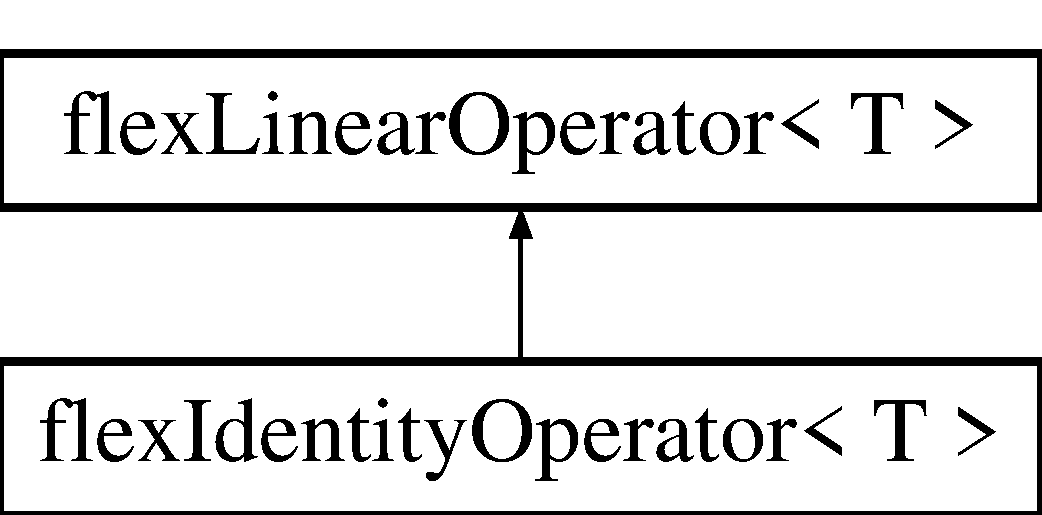
\includegraphics[height=2.000000cm]{classflex_identity_operator}
\end{center}
\end{figure}
\subsection*{Public Member Functions}
\begin{DoxyCompactItemize}
\item 
\hyperlink{classflex_identity_operator_acd55573556fc2313b0280f54c7a6730a}{flex\+Identity\+Operator} (int a\+Num\+Rows, int a\+Num\+Cols, bool a\+Minus)
\begin{DoxyCompactList}\small\item\em initializes the identiy operator \end{DoxyCompactList}\item 
\hyperlink{classflex_identity_operator}{flex\+Identity\+Operator}$<$ T $>$ $\ast$ \hyperlink{classflex_identity_operator_abbd34b97e3e014f02629a68a02f5c41b}{copy} ()
\begin{DoxyCompactList}\small\item\em copies the linear operator \end{DoxyCompactList}\item 
void \hyperlink{classflex_identity_operator_a97ec4aaba5d98227a9865110ad2e7641}{times} (bool transposed, const Tdata \&input, Tdata \&output)
\begin{DoxyCompactList}\small\item\em applies linear operator on vector \end{DoxyCompactList}\item 
void \hyperlink{classflex_identity_operator_a373447505ab85d4d2cf5267fbd03a9d9}{times\+Plus} (bool transposed, const Tdata \&input, Tdata \&output)
\begin{DoxyCompactList}\small\item\em applies linear operator on vector and adds its result to y \end{DoxyCompactList}\item 
void \hyperlink{classflex_identity_operator_a931f2e5ac3651a7f89e78213f08484e9}{times\+Minus} (bool transposed, const Tdata \&input, Tdata \&output)
\begin{DoxyCompactList}\small\item\em applies linear operator on vector and substracts its result from y \end{DoxyCompactList}\item 
T \hyperlink{classflex_identity_operator_ac9127077af24910e90eb0239a2508306}{get\+Max\+Row\+Sum\+Abs} (bool transposed)
\begin{DoxyCompactList}\small\item\em returns the maximum sum of absolute values per row used for preconditioning \end{DoxyCompactList}\item 
std\+::vector$<$ T $>$ \hyperlink{classflex_identity_operator_afe7f2f91fc5f563c2261937f272c0255}{get\+Abs\+Row\+Sum} (bool transposed)
\begin{DoxyCompactList}\small\item\em returns a vector of sum of absolute values per row used for preconditioning \end{DoxyCompactList}\item 
thrust\+::device\+\_\+vector$<$ T $>$ \hyperlink{classflex_identity_operator_ae12ebab61f7f39b0d1f636ad1d27c77a}{get\+Abs\+Row\+Sum\+C\+U\+DA} (bool transposed)
\begin{DoxyCompactList}\small\item\em same function as \hyperlink{classflex_identity_operator_afe7f2f91fc5f563c2261937f272c0255}{get\+Abs\+Row\+Sum()} but implemented in C\+U\+DA \end{DoxyCompactList}\end{DoxyCompactItemize}
\subsection*{Additional Inherited Members}


\subsection{Detailed Description}
\subsubsection*{template$<$typename T$>$\newline
class flex\+Identity\+Operator$<$ T $>$}

represents an identiy operator 

\subsection{Constructor \& Destructor Documentation}
\mbox{\Hypertarget{classflex_identity_operator_acd55573556fc2313b0280f54c7a6730a}\label{classflex_identity_operator_acd55573556fc2313b0280f54c7a6730a}} 
\index{flex\+Identity\+Operator@{flex\+Identity\+Operator}!flex\+Identity\+Operator@{flex\+Identity\+Operator}}
\index{flex\+Identity\+Operator@{flex\+Identity\+Operator}!flex\+Identity\+Operator@{flex\+Identity\+Operator}}
\subsubsection{\texorpdfstring{flex\+Identity\+Operator()}{flexIdentityOperator()}}
{\footnotesize\ttfamily template$<$typename T$>$ \\
\hyperlink{classflex_identity_operator}{flex\+Identity\+Operator}$<$ T $>$\+::\hyperlink{classflex_identity_operator}{flex\+Identity\+Operator} (\begin{DoxyParamCaption}\item[{int}]{a\+Num\+Rows,  }\item[{int}]{a\+Num\+Cols,  }\item[{bool}]{a\+Minus }\end{DoxyParamCaption})\hspace{0.3cm}{\ttfamily [inline]}}



initializes the identiy operator 


\begin{DoxyParams}{Parameters}
{\em a\+Num\+Rows} & number of rows \\
\hline
{\em a\+Num\+Cols} & number of cols \\
\hline
{\em a\+Minus} & determines if operator is negated \\
\hline
\end{DoxyParams}
\begin{DoxySeeAlso}{See also}
\hyperlink{classflex_linear_operator_a7f986517e10aee21099ec7692b77905d}{is\+Minus} 
\end{DoxySeeAlso}


\subsection{Member Function Documentation}
\mbox{\Hypertarget{classflex_identity_operator_abbd34b97e3e014f02629a68a02f5c41b}\label{classflex_identity_operator_abbd34b97e3e014f02629a68a02f5c41b}} 
\index{flex\+Identity\+Operator@{flex\+Identity\+Operator}!copy@{copy}}
\index{copy@{copy}!flex\+Identity\+Operator@{flex\+Identity\+Operator}}
\subsubsection{\texorpdfstring{copy()}{copy()}}
{\footnotesize\ttfamily template$<$typename T$>$ \\
\hyperlink{classflex_identity_operator}{flex\+Identity\+Operator}$<$T$>$$\ast$ \hyperlink{classflex_identity_operator}{flex\+Identity\+Operator}$<$ T $>$\+::copy (\begin{DoxyParamCaption}{ }\end{DoxyParamCaption})\hspace{0.3cm}{\ttfamily [inline]}, {\ttfamily [virtual]}}



copies the linear operator 

\begin{DoxyReturn}{Returns}
copy of linear operator 
\end{DoxyReturn}


Implements \hyperlink{classflex_linear_operator_a7cc1425677cc30fcbd092ffd28d508c9}{flex\+Linear\+Operator$<$ T $>$}.

\mbox{\Hypertarget{classflex_identity_operator_afe7f2f91fc5f563c2261937f272c0255}\label{classflex_identity_operator_afe7f2f91fc5f563c2261937f272c0255}} 
\index{flex\+Identity\+Operator@{flex\+Identity\+Operator}!get\+Abs\+Row\+Sum@{get\+Abs\+Row\+Sum}}
\index{get\+Abs\+Row\+Sum@{get\+Abs\+Row\+Sum}!flex\+Identity\+Operator@{flex\+Identity\+Operator}}
\subsubsection{\texorpdfstring{get\+Abs\+Row\+Sum()}{getAbsRowSum()}}
{\footnotesize\ttfamily template$<$typename T$>$ \\
std\+::vector$<$T$>$ \hyperlink{classflex_identity_operator}{flex\+Identity\+Operator}$<$ T $>$\+::get\+Abs\+Row\+Sum (\begin{DoxyParamCaption}\item[{bool}]{transposed }\end{DoxyParamCaption})\hspace{0.3cm}{\ttfamily [inline]}, {\ttfamily [virtual]}}



returns a vector of sum of absolute values per row used for preconditioning 


\begin{DoxyParams}{Parameters}
{\em transposed} & is true if operator should be (temporarily) transposed before usage \\
\hline
\end{DoxyParams}
\begin{DoxyReturn}{Returns}
vector of sum of absolute values per row 
\end{DoxyReturn}


Implements \hyperlink{classflex_linear_operator_ad6caa7b09e6e3c401cadef61b8e2307e}{flex\+Linear\+Operator$<$ T $>$}.

\mbox{\Hypertarget{classflex_identity_operator_ae12ebab61f7f39b0d1f636ad1d27c77a}\label{classflex_identity_operator_ae12ebab61f7f39b0d1f636ad1d27c77a}} 
\index{flex\+Identity\+Operator@{flex\+Identity\+Operator}!get\+Abs\+Row\+Sum\+C\+U\+DA@{get\+Abs\+Row\+Sum\+C\+U\+DA}}
\index{get\+Abs\+Row\+Sum\+C\+U\+DA@{get\+Abs\+Row\+Sum\+C\+U\+DA}!flex\+Identity\+Operator@{flex\+Identity\+Operator}}
\subsubsection{\texorpdfstring{get\+Abs\+Row\+Sum\+C\+U\+D\+A()}{getAbsRowSumCUDA()}}
{\footnotesize\ttfamily template$<$typename T$>$ \\
thrust\+::device\+\_\+vector$<$T$>$ \hyperlink{classflex_identity_operator}{flex\+Identity\+Operator}$<$ T $>$\+::get\+Abs\+Row\+Sum\+C\+U\+DA (\begin{DoxyParamCaption}\item[{bool}]{transposed }\end{DoxyParamCaption})\hspace{0.3cm}{\ttfamily [inline]}, {\ttfamily [virtual]}}



same function as \hyperlink{classflex_identity_operator_afe7f2f91fc5f563c2261937f272c0255}{get\+Abs\+Row\+Sum()} but implemented in C\+U\+DA 


\begin{DoxyParams}{Parameters}
{\em transposed} & is true if operator should be (temporarily) transposed before usage \\
\hline
\end{DoxyParams}
\begin{DoxyReturn}{Returns}
vector of sum of absolute values per row 
\end{DoxyReturn}


Implements \hyperlink{classflex_linear_operator_a0a0a431d43f4f9d36cbee0d31ba5a29b}{flex\+Linear\+Operator$<$ T $>$}.

\mbox{\Hypertarget{classflex_identity_operator_ac9127077af24910e90eb0239a2508306}\label{classflex_identity_operator_ac9127077af24910e90eb0239a2508306}} 
\index{flex\+Identity\+Operator@{flex\+Identity\+Operator}!get\+Max\+Row\+Sum\+Abs@{get\+Max\+Row\+Sum\+Abs}}
\index{get\+Max\+Row\+Sum\+Abs@{get\+Max\+Row\+Sum\+Abs}!flex\+Identity\+Operator@{flex\+Identity\+Operator}}
\subsubsection{\texorpdfstring{get\+Max\+Row\+Sum\+Abs()}{getMaxRowSumAbs()}}
{\footnotesize\ttfamily template$<$typename T$>$ \\
T \hyperlink{classflex_identity_operator}{flex\+Identity\+Operator}$<$ T $>$\+::get\+Max\+Row\+Sum\+Abs (\begin{DoxyParamCaption}\item[{bool}]{transposed }\end{DoxyParamCaption})\hspace{0.3cm}{\ttfamily [inline]}, {\ttfamily [virtual]}}



returns the maximum sum of absolute values per row used for preconditioning 


\begin{DoxyParams}{Parameters}
{\em transposed} & is true if operator should be (temporarily) transposed before usage \\
\hline
\end{DoxyParams}
\begin{DoxyReturn}{Returns}
maximum sum of absolute values per row 
\end{DoxyReturn}


Implements \hyperlink{classflex_linear_operator_afcb74697385ccb7c8d29870d7034c12a}{flex\+Linear\+Operator$<$ T $>$}.

\mbox{\Hypertarget{classflex_identity_operator_a97ec4aaba5d98227a9865110ad2e7641}\label{classflex_identity_operator_a97ec4aaba5d98227a9865110ad2e7641}} 
\index{flex\+Identity\+Operator@{flex\+Identity\+Operator}!times@{times}}
\index{times@{times}!flex\+Identity\+Operator@{flex\+Identity\+Operator}}
\subsubsection{\texorpdfstring{times()}{times()}}
{\footnotesize\ttfamily template$<$typename T$>$ \\
void \hyperlink{classflex_identity_operator}{flex\+Identity\+Operator}$<$ T $>$\+::times (\begin{DoxyParamCaption}\item[{bool}]{transposed,  }\item[{const Tdata \&}]{input,  }\item[{Tdata \&}]{output }\end{DoxyParamCaption})\hspace{0.3cm}{\ttfamily [inline]}, {\ttfamily [virtual]}}



applies linear operator on vector 

equals $ y = Ax $ 
\begin{DoxyParams}{Parameters}
{\em transposed} & is true if operator should be (temporarily) transposed before usage \\
\hline
{\em input} & data to be processed \\
\hline
{\em output} & output data \\
\hline
\end{DoxyParams}


Implements \hyperlink{classflex_linear_operator_a883982edf3be857815d2095e53f76e75}{flex\+Linear\+Operator$<$ T $>$}.

\mbox{\Hypertarget{classflex_identity_operator_a931f2e5ac3651a7f89e78213f08484e9}\label{classflex_identity_operator_a931f2e5ac3651a7f89e78213f08484e9}} 
\index{flex\+Identity\+Operator@{flex\+Identity\+Operator}!times\+Minus@{times\+Minus}}
\index{times\+Minus@{times\+Minus}!flex\+Identity\+Operator@{flex\+Identity\+Operator}}
\subsubsection{\texorpdfstring{times\+Minus()}{timesMinus()}}
{\footnotesize\ttfamily template$<$typename T$>$ \\
void \hyperlink{classflex_identity_operator}{flex\+Identity\+Operator}$<$ T $>$\+::times\+Minus (\begin{DoxyParamCaption}\item[{bool}]{transposed,  }\item[{const Tdata \&}]{input,  }\item[{Tdata \&}]{output }\end{DoxyParamCaption})\hspace{0.3cm}{\ttfamily [inline]}, {\ttfamily [virtual]}}



applies linear operator on vector and substracts its result from y 

equals $ y = y - Ax $ 
\begin{DoxyParams}{Parameters}
{\em transposed} & is true if operator should be (temporarily) transposed before usage \\
\hline
{\em input} & data to be processed \\
\hline
{\em output} & output data \\
\hline
\end{DoxyParams}


Implements \hyperlink{classflex_linear_operator_a62708874e134a649c8445df333079c69}{flex\+Linear\+Operator$<$ T $>$}.

\mbox{\Hypertarget{classflex_identity_operator_a373447505ab85d4d2cf5267fbd03a9d9}\label{classflex_identity_operator_a373447505ab85d4d2cf5267fbd03a9d9}} 
\index{flex\+Identity\+Operator@{flex\+Identity\+Operator}!times\+Plus@{times\+Plus}}
\index{times\+Plus@{times\+Plus}!flex\+Identity\+Operator@{flex\+Identity\+Operator}}
\subsubsection{\texorpdfstring{times\+Plus()}{timesPlus()}}
{\footnotesize\ttfamily template$<$typename T$>$ \\
void \hyperlink{classflex_identity_operator}{flex\+Identity\+Operator}$<$ T $>$\+::times\+Plus (\begin{DoxyParamCaption}\item[{bool}]{transposed,  }\item[{const Tdata \&}]{input,  }\item[{Tdata \&}]{output }\end{DoxyParamCaption})\hspace{0.3cm}{\ttfamily [inline]}, {\ttfamily [virtual]}}



applies linear operator on vector and adds its result to y 

equals $ y = y + Ax $ 
\begin{DoxyParams}{Parameters}
{\em transposed} & is true if operator should be (temporarily) transposed before usage \\
\hline
{\em input} & data to be processed \\
\hline
{\em output} & output data \\
\hline
\end{DoxyParams}


Implements \hyperlink{classflex_linear_operator_a3f2978ad1c5eae8cd4ae16deb2337416}{flex\+Linear\+Operator$<$ T $>$}.



The documentation for this class was generated from the following file\+:\begin{DoxyCompactItemize}
\item 
flex\+Identity\+Operator.\+h\end{DoxyCompactItemize}

\hypertarget{classflex_linear_operator}{}\section{flex\+Linear\+Operator$<$ T $>$ Class Template Reference}
\label{classflex_linear_operator}\index{flex\+Linear\+Operator$<$ T $>$@{flex\+Linear\+Operator$<$ T $>$}}


abstract base class for linear operators  




{\ttfamily \#include $<$flex\+Linear\+Operator.\+h$>$}

Inheritance diagram for flex\+Linear\+Operator$<$ T $>$\+:\begin{figure}[H]
\begin{center}
\leavevmode
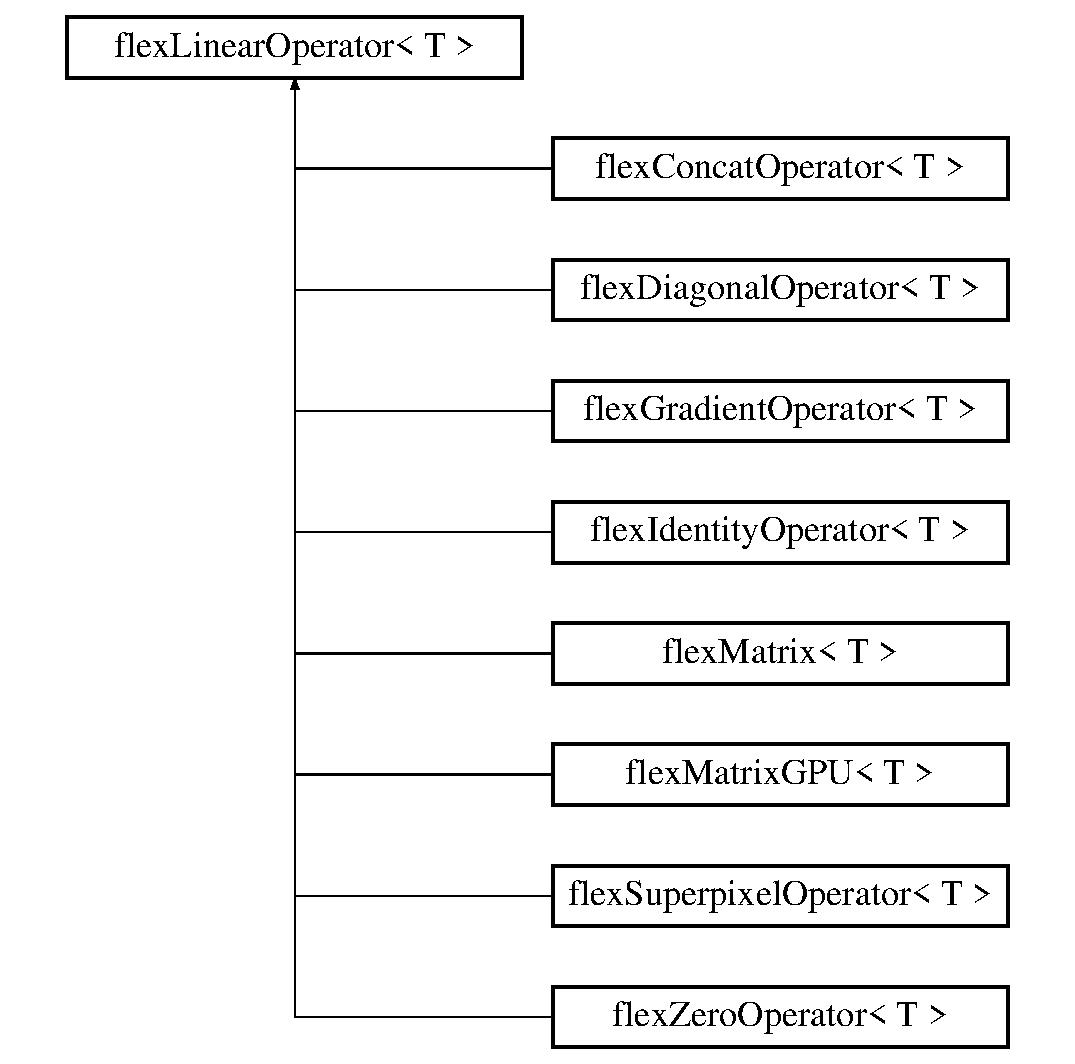
\includegraphics[height=11.000000cm]{classflex_linear_operator}
\end{center}
\end{figure}
\subsection*{Public Member Functions}
\begin{DoxyCompactItemize}
\item 
\hyperlink{classflex_linear_operator_ab4a525e1069965d018b8f4371db60234}{flex\+Linear\+Operator} (int a\+Num\+Rows, int a\+Num\+Cols, \hyperlink{tools_8h_a3fc67a2f9370c09fecbd90da67687d36}{lin\+Op} a\+Type, bool a\+Is\+Minus)
\begin{DoxyCompactList}\small\item\em initializes the linear operator \end{DoxyCompactList}\item 
int \hyperlink{classflex_linear_operator_add18da4274ec9105f7ba8852be35201a}{get\+Num\+Cols} () const
\begin{DoxyCompactList}\small\item\em returns number of columns of the linear operator \end{DoxyCompactList}\item 
int \hyperlink{classflex_linear_operator_a6f807b6a0549a79cb22598ab0c42ef21}{get\+Num\+Rows} () const
\begin{DoxyCompactList}\small\item\em returns number of rows of the linear operator \end{DoxyCompactList}\item 
void \hyperlink{classflex_linear_operator_add43d72e6e24ff2690fc3f1ea2578818}{set\+Num\+Cols} (int a\+Num\+Cols)
\begin{DoxyCompactList}\small\item\em sets the number of columns of the linear operator \end{DoxyCompactList}\item 
void \hyperlink{classflex_linear_operator_a14ea80aaa2a6d3c468f6bf38452f1001}{set\+Num\+Rows} (int a\+Num\+Rows)
\begin{DoxyCompactList}\small\item\em sets the number of rows of the linear operator \end{DoxyCompactList}\item 
void \hyperlink{classflex_linear_operator_a0757a5f739ef85162cfc95e40eeb7784}{set\+Minus} (bool a\+Is\+Minus)
\begin{DoxyCompactList}\small\item\em constrols if operator should be negated or not \end{DoxyCompactList}\item 
virtual \hyperlink{classflex_linear_operator}{flex\+Linear\+Operator}$<$ T $>$ $\ast$ \hyperlink{classflex_linear_operator_a7cc1425677cc30fcbd092ffd28d508c9}{copy} ()=0
\begin{DoxyCompactList}\small\item\em copies the linear operator \end{DoxyCompactList}\item 
virtual void \hyperlink{classflex_linear_operator_a883982edf3be857815d2095e53f76e75}{times} (bool transposed, const Tdata \&input, Tdata \&output)=0
\begin{DoxyCompactList}\small\item\em applies linear operator on vector \end{DoxyCompactList}\item 
virtual void \hyperlink{classflex_linear_operator_a3f2978ad1c5eae8cd4ae16deb2337416}{times\+Plus} (bool transposed, const Tdata \&input, Tdata \&output)=0
\begin{DoxyCompactList}\small\item\em applies linear operator on vector and adds its result to y \end{DoxyCompactList}\item 
virtual void \hyperlink{classflex_linear_operator_a62708874e134a649c8445df333079c69}{times\+Minus} (bool transposed, const Tdata \&input, Tdata \&output)=0
\begin{DoxyCompactList}\small\item\em applies linear operator on vector and substracts its result from y \end{DoxyCompactList}\item 
virtual std\+::vector$<$ T $>$ \hyperlink{classflex_linear_operator_ad6caa7b09e6e3c401cadef61b8e2307e}{get\+Abs\+Row\+Sum} (bool transposed)=0
\begin{DoxyCompactList}\small\item\em returns a vector of sum of absolute values per row used for preconditioning \end{DoxyCompactList}\item 
virtual thrust\+::device\+\_\+vector$<$ T $>$ \hyperlink{classflex_linear_operator_a0a0a431d43f4f9d36cbee0d31ba5a29b}{get\+Abs\+Row\+Sum\+C\+U\+DA} (bool transposed)=0
\begin{DoxyCompactList}\small\item\em same function as \hyperlink{classflex_linear_operator_ad6caa7b09e6e3c401cadef61b8e2307e}{get\+Abs\+Row\+Sum()} but implemented in C\+U\+DA \end{DoxyCompactList}\item 
virtual T \hyperlink{classflex_linear_operator_afcb74697385ccb7c8d29870d7034c12a}{get\+Max\+Row\+Sum\+Abs} (bool transposed)=0
\begin{DoxyCompactList}\small\item\em returns the maximum sum of absolute values per row used for preconditioning \end{DoxyCompactList}\end{DoxyCompactItemize}
\subsection*{Public Attributes}
\begin{DoxyCompactItemize}
\item 
\hyperlink{tools_8h_a3fc67a2f9370c09fecbd90da67687d36}{lin\+Op} \hyperlink{classflex_linear_operator_a80b240d65c64cb9843e28da602995940}{type}
\begin{DoxyCompactList}\small\item\em type of linear operator \end{DoxyCompactList}\item 
\mbox{\Hypertarget{classflex_linear_operator_a7f986517e10aee21099ec7692b77905d}\label{classflex_linear_operator_a7f986517e10aee21099ec7692b77905d}} 
bool \hyperlink{classflex_linear_operator_a7f986517e10aee21099ec7692b77905d}{is\+Minus}
\begin{DoxyCompactList}\small\item\em determines if operator is negated \end{DoxyCompactList}\end{DoxyCompactItemize}


\subsection{Detailed Description}
\subsubsection*{template$<$typename T$>$\newline
class flex\+Linear\+Operator$<$ T $>$}

abstract base class for linear operators 

\hyperlink{classflex_linear_operator}{flex\+Linear\+Operator} combines the interface for all usable operators 

\subsection{Constructor \& Destructor Documentation}
\mbox{\Hypertarget{classflex_linear_operator_ab4a525e1069965d018b8f4371db60234}\label{classflex_linear_operator_ab4a525e1069965d018b8f4371db60234}} 
\index{flex\+Linear\+Operator@{flex\+Linear\+Operator}!flex\+Linear\+Operator@{flex\+Linear\+Operator}}
\index{flex\+Linear\+Operator@{flex\+Linear\+Operator}!flex\+Linear\+Operator@{flex\+Linear\+Operator}}
\subsubsection{\texorpdfstring{flex\+Linear\+Operator()}{flexLinearOperator()}}
{\footnotesize\ttfamily template$<$typename T$>$ \\
\hyperlink{classflex_linear_operator}{flex\+Linear\+Operator}$<$ T $>$\+::\hyperlink{classflex_linear_operator}{flex\+Linear\+Operator} (\begin{DoxyParamCaption}\item[{int}]{a\+Num\+Rows,  }\item[{int}]{a\+Num\+Cols,  }\item[{\hyperlink{tools_8h_a3fc67a2f9370c09fecbd90da67687d36}{lin\+Op}}]{a\+Type,  }\item[{bool}]{a\+Is\+Minus }\end{DoxyParamCaption})\hspace{0.3cm}{\ttfamily [inline]}}



initializes the linear operator 


\begin{DoxyParams}{Parameters}
{\em a\+Num\+Rows} & number of rows of liner operator \\
\hline
{\em a\+Num\+Cols} & number of columns of liner operator \\
\hline
{\em a\+Type} & type of linear operator sa type \\
\hline
\end{DoxyParams}
\begin{DoxySeeAlso}{See also}
\hyperlink{classflex_linear_operator_a80b240d65c64cb9843e28da602995940}{type} 
\end{DoxySeeAlso}

\begin{DoxyParams}{Parameters}
{\em a\+Is\+Minus} & determines if operator is negated \\
\hline
\end{DoxyParams}
\begin{DoxySeeAlso}{See also}
\hyperlink{classflex_linear_operator_a7f986517e10aee21099ec7692b77905d}{is\+Minus} 
\end{DoxySeeAlso}


\subsection{Member Function Documentation}
\mbox{\Hypertarget{classflex_linear_operator_a7cc1425677cc30fcbd092ffd28d508c9}\label{classflex_linear_operator_a7cc1425677cc30fcbd092ffd28d508c9}} 
\index{flex\+Linear\+Operator@{flex\+Linear\+Operator}!copy@{copy}}
\index{copy@{copy}!flex\+Linear\+Operator@{flex\+Linear\+Operator}}
\subsubsection{\texorpdfstring{copy()}{copy()}}
{\footnotesize\ttfamily template$<$typename T$>$ \\
virtual \hyperlink{classflex_linear_operator}{flex\+Linear\+Operator}$<$T$>$$\ast$ \hyperlink{classflex_linear_operator}{flex\+Linear\+Operator}$<$ T $>$\+::copy (\begin{DoxyParamCaption}{ }\end{DoxyParamCaption})\hspace{0.3cm}{\ttfamily [pure virtual]}}



copies the linear operator 

\begin{DoxyReturn}{Returns}
copy of linear operator 
\end{DoxyReturn}


Implemented in \hyperlink{classflex_gradient_operator_a4b1480051ac7763da809c509685316d2}{flex\+Gradient\+Operator$<$ T $>$}, \hyperlink{classflex_matrix_g_p_u_a4df27ef284eec123ba72f1b5788f1180}{flex\+Matrix\+G\+P\+U$<$ T $>$}, \hyperlink{classflex_diagonal_operator_aeca7325de5eaface63363e9710034128}{flex\+Diagonal\+Operator$<$ T $>$}, \hyperlink{classflex_concat_operator_a8e554cb6edb47de0cf922cf51ec398b5}{flex\+Concat\+Operator$<$ T $>$}, \hyperlink{classflex_superpixel_operator_ab0e066735127a3b39958c6719fe03156}{flex\+Superpixel\+Operator$<$ T $>$}, \hyperlink{classflex_matrix_a4e9d53b8d606511759decbf52628203a}{flex\+Matrix$<$ T $>$}, \hyperlink{classflex_matrix_logical_a25c9ecc21cfccc07e1390c554784ee27}{flex\+Matrix\+Logical$<$ T $>$}, \hyperlink{classflex_full_matrix_a849d2974a11456c6a23801f51838bc7b}{flex\+Full\+Matrix$<$ T $>$}, \hyperlink{classflex_identity_operator_abbd34b97e3e014f02629a68a02f5c41b}{flex\+Identity\+Operator$<$ T $>$}, and \hyperlink{classflex_zero_operator_ab26ce548041980be572f7972907397af}{flex\+Zero\+Operator$<$ T $>$}.

\mbox{\Hypertarget{classflex_linear_operator_ad6caa7b09e6e3c401cadef61b8e2307e}\label{classflex_linear_operator_ad6caa7b09e6e3c401cadef61b8e2307e}} 
\index{flex\+Linear\+Operator@{flex\+Linear\+Operator}!get\+Abs\+Row\+Sum@{get\+Abs\+Row\+Sum}}
\index{get\+Abs\+Row\+Sum@{get\+Abs\+Row\+Sum}!flex\+Linear\+Operator@{flex\+Linear\+Operator}}
\subsubsection{\texorpdfstring{get\+Abs\+Row\+Sum()}{getAbsRowSum()}}
{\footnotesize\ttfamily template$<$typename T$>$ \\
virtual std\+::vector$<$T$>$ \hyperlink{classflex_linear_operator}{flex\+Linear\+Operator}$<$ T $>$\+::get\+Abs\+Row\+Sum (\begin{DoxyParamCaption}\item[{bool}]{transposed }\end{DoxyParamCaption})\hspace{0.3cm}{\ttfamily [pure virtual]}}



returns a vector of sum of absolute values per row used for preconditioning 


\begin{DoxyParams}{Parameters}
{\em transposed} & is true if operator should be (temporarily) transposed before usage \\
\hline
\end{DoxyParams}
\begin{DoxyReturn}{Returns}
vector of sum of absolute values per row 
\end{DoxyReturn}


Implemented in \hyperlink{classflex_gradient_operator_a04950a1e57f7587b95824bfd82b35738}{flex\+Gradient\+Operator$<$ T $>$}, \hyperlink{classflex_matrix_g_p_u_a0a1f19c482243223b8d98165d0b44ccf}{flex\+Matrix\+G\+P\+U$<$ T $>$}, \hyperlink{classflex_concat_operator_a6cae0c9545cf1afd8ac0ebc418fa3327}{flex\+Concat\+Operator$<$ T $>$}, \hyperlink{classflex_matrix_a75f378787fc81ea2c570c9848a7f2588}{flex\+Matrix$<$ T $>$}, \hyperlink{classflex_matrix_logical_a0c7cf2e5dde3a2d55ae95c6e54f94342}{flex\+Matrix\+Logical$<$ T $>$}, \hyperlink{classflex_diagonal_operator_ad53cb526b55141a1d0519a023572cf58}{flex\+Diagonal\+Operator$<$ T $>$}, \hyperlink{classflex_identity_operator_afe7f2f91fc5f563c2261937f272c0255}{flex\+Identity\+Operator$<$ T $>$}, \hyperlink{classflex_full_matrix_a911d6b2a452edb8233f56c1e5250855e}{flex\+Full\+Matrix$<$ T $>$}, \hyperlink{classflex_superpixel_operator_afd3f55401eaa6fb3e8a62c7f83443a4d}{flex\+Superpixel\+Operator$<$ T $>$}, and \hyperlink{classflex_zero_operator_a4c9fbbcd1961590e2fabef75197f4367}{flex\+Zero\+Operator$<$ T $>$}.

\mbox{\Hypertarget{classflex_linear_operator_a0a0a431d43f4f9d36cbee0d31ba5a29b}\label{classflex_linear_operator_a0a0a431d43f4f9d36cbee0d31ba5a29b}} 
\index{flex\+Linear\+Operator@{flex\+Linear\+Operator}!get\+Abs\+Row\+Sum\+C\+U\+DA@{get\+Abs\+Row\+Sum\+C\+U\+DA}}
\index{get\+Abs\+Row\+Sum\+C\+U\+DA@{get\+Abs\+Row\+Sum\+C\+U\+DA}!flex\+Linear\+Operator@{flex\+Linear\+Operator}}
\subsubsection{\texorpdfstring{get\+Abs\+Row\+Sum\+C\+U\+D\+A()}{getAbsRowSumCUDA()}}
{\footnotesize\ttfamily template$<$typename T$>$ \\
virtual thrust\+::device\+\_\+vector$<$T$>$ \hyperlink{classflex_linear_operator}{flex\+Linear\+Operator}$<$ T $>$\+::get\+Abs\+Row\+Sum\+C\+U\+DA (\begin{DoxyParamCaption}\item[{bool}]{transposed }\end{DoxyParamCaption})\hspace{0.3cm}{\ttfamily [pure virtual]}}



same function as \hyperlink{classflex_linear_operator_ad6caa7b09e6e3c401cadef61b8e2307e}{get\+Abs\+Row\+Sum()} but implemented in C\+U\+DA 


\begin{DoxyParams}{Parameters}
{\em transposed} & is true if operator should be (temporarily) transposed before usage \\
\hline
\end{DoxyParams}
\begin{DoxyReturn}{Returns}
vector of sum of absolute values per row 
\end{DoxyReturn}


Implemented in \hyperlink{classflex_gradient_operator_ac5cf151db87946ac0f1864344db260d5}{flex\+Gradient\+Operator$<$ T $>$}, \hyperlink{classflex_matrix_g_p_u_ab9fceb951d911794d4c70f5045255abd}{flex\+Matrix\+G\+P\+U$<$ T $>$}, \hyperlink{classflex_concat_operator_a76e35865b16975bfcd6431879bda195b}{flex\+Concat\+Operator$<$ T $>$}, \hyperlink{classflex_matrix_ae713d5dabcdab30df9b04f2a7d499235}{flex\+Matrix$<$ T $>$}, \hyperlink{classflex_matrix_logical_a0245c73fb7d1fb3b1900208e0deb48d6}{flex\+Matrix\+Logical$<$ T $>$}, \hyperlink{classflex_full_matrix_af8ade69023e1c5140a82ad3583a8acb6}{flex\+Full\+Matrix$<$ T $>$}, \hyperlink{classflex_diagonal_operator_a71cdb6ea6b8b7ceabaf538a180c8dcf4}{flex\+Diagonal\+Operator$<$ T $>$}, \hyperlink{classflex_identity_operator_ae12ebab61f7f39b0d1f636ad1d27c77a}{flex\+Identity\+Operator$<$ T $>$}, \hyperlink{classflex_superpixel_operator_ae2f878d68c4574a0d5f21ffd132afc63}{flex\+Superpixel\+Operator$<$ T $>$}, and \hyperlink{classflex_zero_operator_ad63f43f4b1abe71779e5b0ee364b93d1}{flex\+Zero\+Operator$<$ T $>$}.

\mbox{\Hypertarget{classflex_linear_operator_afcb74697385ccb7c8d29870d7034c12a}\label{classflex_linear_operator_afcb74697385ccb7c8d29870d7034c12a}} 
\index{flex\+Linear\+Operator@{flex\+Linear\+Operator}!get\+Max\+Row\+Sum\+Abs@{get\+Max\+Row\+Sum\+Abs}}
\index{get\+Max\+Row\+Sum\+Abs@{get\+Max\+Row\+Sum\+Abs}!flex\+Linear\+Operator@{flex\+Linear\+Operator}}
\subsubsection{\texorpdfstring{get\+Max\+Row\+Sum\+Abs()}{getMaxRowSumAbs()}}
{\footnotesize\ttfamily template$<$typename T$>$ \\
virtual T \hyperlink{classflex_linear_operator}{flex\+Linear\+Operator}$<$ T $>$\+::get\+Max\+Row\+Sum\+Abs (\begin{DoxyParamCaption}\item[{bool}]{transposed }\end{DoxyParamCaption})\hspace{0.3cm}{\ttfamily [pure virtual]}}



returns the maximum sum of absolute values per row used for preconditioning 


\begin{DoxyParams}{Parameters}
{\em transposed} & is true if operator should be (temporarily) transposed before usage \\
\hline
\end{DoxyParams}
\begin{DoxyReturn}{Returns}
maximum sum of absolute values per row 
\end{DoxyReturn}


Implemented in \hyperlink{classflex_gradient_operator_a6acb61ea8abf404d63be4574976391bb}{flex\+Gradient\+Operator$<$ T $>$}, \hyperlink{classflex_matrix_g_p_u_aae4f81a403b6fff8ac73ccdf6c21399f}{flex\+Matrix\+G\+P\+U$<$ T $>$}, \hyperlink{classflex_concat_operator_a39b7aa1797025fb022630a63358a4072}{flex\+Concat\+Operator$<$ T $>$}, \hyperlink{classflex_matrix_a25cd9571e7056c4ad035a44a57e1d45d}{flex\+Matrix$<$ T $>$}, \hyperlink{classflex_diagonal_operator_aa9c144ae23fbcbcdcd14cc779182896a}{flex\+Diagonal\+Operator$<$ T $>$}, \hyperlink{classflex_matrix_logical_ab35a9ebf590236184573731bb08e176d}{flex\+Matrix\+Logical$<$ T $>$}, \hyperlink{classflex_identity_operator_ac9127077af24910e90eb0239a2508306}{flex\+Identity\+Operator$<$ T $>$}, \hyperlink{classflex_full_matrix_a3ca8466b330c14b23689cb9f5507d40a}{flex\+Full\+Matrix$<$ T $>$}, \hyperlink{classflex_superpixel_operator_a83c4978b05be05c45be7d2ea58e96b44}{flex\+Superpixel\+Operator$<$ T $>$}, and \hyperlink{classflex_zero_operator_a2c7b6c1cddc5a79c4d2948855a20b3f1}{flex\+Zero\+Operator$<$ T $>$}.

\mbox{\Hypertarget{classflex_linear_operator_add18da4274ec9105f7ba8852be35201a}\label{classflex_linear_operator_add18da4274ec9105f7ba8852be35201a}} 
\index{flex\+Linear\+Operator@{flex\+Linear\+Operator}!get\+Num\+Cols@{get\+Num\+Cols}}
\index{get\+Num\+Cols@{get\+Num\+Cols}!flex\+Linear\+Operator@{flex\+Linear\+Operator}}
\subsubsection{\texorpdfstring{get\+Num\+Cols()}{getNumCols()}}
{\footnotesize\ttfamily template$<$typename T$>$ \\
int \hyperlink{classflex_linear_operator}{flex\+Linear\+Operator}$<$ T $>$\+::get\+Num\+Cols (\begin{DoxyParamCaption}{ }\end{DoxyParamCaption}) const\hspace{0.3cm}{\ttfamily [inline]}}



returns number of columns of the linear operator 

\begin{DoxyReturn}{Returns}
number of columns 
\end{DoxyReturn}
\mbox{\Hypertarget{classflex_linear_operator_a6f807b6a0549a79cb22598ab0c42ef21}\label{classflex_linear_operator_a6f807b6a0549a79cb22598ab0c42ef21}} 
\index{flex\+Linear\+Operator@{flex\+Linear\+Operator}!get\+Num\+Rows@{get\+Num\+Rows}}
\index{get\+Num\+Rows@{get\+Num\+Rows}!flex\+Linear\+Operator@{flex\+Linear\+Operator}}
\subsubsection{\texorpdfstring{get\+Num\+Rows()}{getNumRows()}}
{\footnotesize\ttfamily template$<$typename T$>$ \\
int \hyperlink{classflex_linear_operator}{flex\+Linear\+Operator}$<$ T $>$\+::get\+Num\+Rows (\begin{DoxyParamCaption}{ }\end{DoxyParamCaption}) const\hspace{0.3cm}{\ttfamily [inline]}}



returns number of rows of the linear operator 

\begin{DoxyReturn}{Returns}
number of rows 
\end{DoxyReturn}
\mbox{\Hypertarget{classflex_linear_operator_a0757a5f739ef85162cfc95e40eeb7784}\label{classflex_linear_operator_a0757a5f739ef85162cfc95e40eeb7784}} 
\index{flex\+Linear\+Operator@{flex\+Linear\+Operator}!set\+Minus@{set\+Minus}}
\index{set\+Minus@{set\+Minus}!flex\+Linear\+Operator@{flex\+Linear\+Operator}}
\subsubsection{\texorpdfstring{set\+Minus()}{setMinus()}}
{\footnotesize\ttfamily template$<$typename T$>$ \\
void \hyperlink{classflex_linear_operator}{flex\+Linear\+Operator}$<$ T $>$\+::set\+Minus (\begin{DoxyParamCaption}\item[{bool}]{a\+Is\+Minus }\end{DoxyParamCaption})\hspace{0.3cm}{\ttfamily [inline]}}



constrols if operator should be negated or not 


\begin{DoxyParams}{Parameters}
{\em a\+Is\+Minus} & true if operator should be negated, otherwise false. \\
\hline
\end{DoxyParams}
\mbox{\Hypertarget{classflex_linear_operator_add43d72e6e24ff2690fc3f1ea2578818}\label{classflex_linear_operator_add43d72e6e24ff2690fc3f1ea2578818}} 
\index{flex\+Linear\+Operator@{flex\+Linear\+Operator}!set\+Num\+Cols@{set\+Num\+Cols}}
\index{set\+Num\+Cols@{set\+Num\+Cols}!flex\+Linear\+Operator@{flex\+Linear\+Operator}}
\subsubsection{\texorpdfstring{set\+Num\+Cols()}{setNumCols()}}
{\footnotesize\ttfamily template$<$typename T$>$ \\
void \hyperlink{classflex_linear_operator}{flex\+Linear\+Operator}$<$ T $>$\+::set\+Num\+Cols (\begin{DoxyParamCaption}\item[{int}]{a\+Num\+Cols }\end{DoxyParamCaption})\hspace{0.3cm}{\ttfamily [inline]}}



sets the number of columns of the linear operator 


\begin{DoxyParams}{Parameters}
{\em a\+Num\+Cols} & number of columns \\
\hline
\end{DoxyParams}
\mbox{\Hypertarget{classflex_linear_operator_a14ea80aaa2a6d3c468f6bf38452f1001}\label{classflex_linear_operator_a14ea80aaa2a6d3c468f6bf38452f1001}} 
\index{flex\+Linear\+Operator@{flex\+Linear\+Operator}!set\+Num\+Rows@{set\+Num\+Rows}}
\index{set\+Num\+Rows@{set\+Num\+Rows}!flex\+Linear\+Operator@{flex\+Linear\+Operator}}
\subsubsection{\texorpdfstring{set\+Num\+Rows()}{setNumRows()}}
{\footnotesize\ttfamily template$<$typename T$>$ \\
void \hyperlink{classflex_linear_operator}{flex\+Linear\+Operator}$<$ T $>$\+::set\+Num\+Rows (\begin{DoxyParamCaption}\item[{int}]{a\+Num\+Rows }\end{DoxyParamCaption})\hspace{0.3cm}{\ttfamily [inline]}}



sets the number of rows of the linear operator 


\begin{DoxyParams}{Parameters}
{\em a\+Num\+Rows} & number of rows \\
\hline
\end{DoxyParams}
\mbox{\Hypertarget{classflex_linear_operator_a883982edf3be857815d2095e53f76e75}\label{classflex_linear_operator_a883982edf3be857815d2095e53f76e75}} 
\index{flex\+Linear\+Operator@{flex\+Linear\+Operator}!times@{times}}
\index{times@{times}!flex\+Linear\+Operator@{flex\+Linear\+Operator}}
\subsubsection{\texorpdfstring{times()}{times()}}
{\footnotesize\ttfamily template$<$typename T$>$ \\
virtual void \hyperlink{classflex_linear_operator}{flex\+Linear\+Operator}$<$ T $>$\+::times (\begin{DoxyParamCaption}\item[{bool}]{transposed,  }\item[{const Tdata \&}]{input,  }\item[{Tdata \&}]{output }\end{DoxyParamCaption})\hspace{0.3cm}{\ttfamily [pure virtual]}}



applies linear operator on vector 

equals $ y = Ax $ 
\begin{DoxyParams}{Parameters}
{\em transposed} & is true if operator should be (temporarily) transposed before usage \\
\hline
{\em input} & data to be processed \\
\hline
{\em output} & output data \\
\hline
\end{DoxyParams}


Implemented in \hyperlink{classflex_gradient_operator_aae5e807f99c3634c52b79f08d72fa7a2}{flex\+Gradient\+Operator$<$ T $>$}, \hyperlink{classflex_matrix_g_p_u_a059adf49cc4d895d017eed28462a29e4}{flex\+Matrix\+G\+P\+U$<$ T $>$}, \hyperlink{classflex_diagonal_operator_a701d4741eb75d3e63fd47b936b46fb8c}{flex\+Diagonal\+Operator$<$ T $>$}, \hyperlink{classflex_concat_operator_af32c0fc8fc008a965d825dd0607ea388}{flex\+Concat\+Operator$<$ T $>$}, \hyperlink{classflex_matrix_ac7e95eed2025202b252d804034b923b6}{flex\+Matrix$<$ T $>$}, \hyperlink{classflex_matrix_logical_ab1ccf3400da547a27b5753a894905c63}{flex\+Matrix\+Logical$<$ T $>$}, \hyperlink{classflex_superpixel_operator_afa075c0858c693342646250225f7c425}{flex\+Superpixel\+Operator$<$ T $>$}, \hyperlink{classflex_full_matrix_ad5c9cc8d3618cba2f96c963a6d180224}{flex\+Full\+Matrix$<$ T $>$}, \hyperlink{classflex_identity_operator_a97ec4aaba5d98227a9865110ad2e7641}{flex\+Identity\+Operator$<$ T $>$}, and \hyperlink{classflex_zero_operator_a3f512b2a67a803417d280e78418f8243}{flex\+Zero\+Operator$<$ T $>$}.

\mbox{\Hypertarget{classflex_linear_operator_a62708874e134a649c8445df333079c69}\label{classflex_linear_operator_a62708874e134a649c8445df333079c69}} 
\index{flex\+Linear\+Operator@{flex\+Linear\+Operator}!times\+Minus@{times\+Minus}}
\index{times\+Minus@{times\+Minus}!flex\+Linear\+Operator@{flex\+Linear\+Operator}}
\subsubsection{\texorpdfstring{times\+Minus()}{timesMinus()}}
{\footnotesize\ttfamily template$<$typename T$>$ \\
virtual void \hyperlink{classflex_linear_operator}{flex\+Linear\+Operator}$<$ T $>$\+::times\+Minus (\begin{DoxyParamCaption}\item[{bool}]{transposed,  }\item[{const Tdata \&}]{input,  }\item[{Tdata \&}]{output }\end{DoxyParamCaption})\hspace{0.3cm}{\ttfamily [pure virtual]}}



applies linear operator on vector and substracts its result from y 

equals $ y = y - Ax $ 
\begin{DoxyParams}{Parameters}
{\em transposed} & is true if operator should be (temporarily) transposed before usage \\
\hline
{\em input} & data to be processed \\
\hline
{\em output} & output data \\
\hline
\end{DoxyParams}


Implemented in \hyperlink{classflex_gradient_operator_a287f5efd41aa14ee61aee87dfed08b88}{flex\+Gradient\+Operator$<$ T $>$}, \hyperlink{classflex_matrix_g_p_u_a4d6b328bba4170827a1ead228ecd8fcb}{flex\+Matrix\+G\+P\+U$<$ T $>$}, \hyperlink{classflex_concat_operator_a270c30ae4a8420729348eba8051ee322}{flex\+Concat\+Operator$<$ T $>$}, \hyperlink{classflex_diagonal_operator_ac579880d56e9703a5fcb6cafbf9fe338}{flex\+Diagonal\+Operator$<$ T $>$}, \hyperlink{classflex_identity_operator_a931f2e5ac3651a7f89e78213f08484e9}{flex\+Identity\+Operator$<$ T $>$}, \hyperlink{classflex_matrix_a100e59f7261d95eabc28fd9056d2b77b}{flex\+Matrix$<$ T $>$}, \hyperlink{classflex_matrix_logical_a7f3b3d9f007696d7140c2f2256de8dd8}{flex\+Matrix\+Logical$<$ T $>$}, \hyperlink{classflex_superpixel_operator_af0831ae77a7e8c894a110146a316c944}{flex\+Superpixel\+Operator$<$ T $>$}, \hyperlink{classflex_full_matrix_adf676d913b1409d6792fcd6cce144285}{flex\+Full\+Matrix$<$ T $>$}, and \hyperlink{classflex_zero_operator_ae1b71503e1c6bf070deb080f2a0f1dd4}{flex\+Zero\+Operator$<$ T $>$}.

\mbox{\Hypertarget{classflex_linear_operator_a3f2978ad1c5eae8cd4ae16deb2337416}\label{classflex_linear_operator_a3f2978ad1c5eae8cd4ae16deb2337416}} 
\index{flex\+Linear\+Operator@{flex\+Linear\+Operator}!times\+Plus@{times\+Plus}}
\index{times\+Plus@{times\+Plus}!flex\+Linear\+Operator@{flex\+Linear\+Operator}}
\subsubsection{\texorpdfstring{times\+Plus()}{timesPlus()}}
{\footnotesize\ttfamily template$<$typename T$>$ \\
virtual void \hyperlink{classflex_linear_operator}{flex\+Linear\+Operator}$<$ T $>$\+::times\+Plus (\begin{DoxyParamCaption}\item[{bool}]{transposed,  }\item[{const Tdata \&}]{input,  }\item[{Tdata \&}]{output }\end{DoxyParamCaption})\hspace{0.3cm}{\ttfamily [pure virtual]}}



applies linear operator on vector and adds its result to y 

equals $ y = y + Ax $ 
\begin{DoxyParams}{Parameters}
{\em transposed} & is true if operator should be (temporarily) transposed before usage \\
\hline
{\em input} & data to be processed \\
\hline
{\em output} & output data \\
\hline
\end{DoxyParams}


Implemented in \hyperlink{classflex_gradient_operator_a1b6c9b788e6d5a62ba008811f287f8e5}{flex\+Gradient\+Operator$<$ T $>$}, \hyperlink{classflex_matrix_g_p_u_adbb111427c3bc8ef6157ba60b3dbea3d}{flex\+Matrix\+G\+P\+U$<$ T $>$}, \hyperlink{classflex_diagonal_operator_ab8b9999592b97c6189f7f2c5d3bd47af}{flex\+Diagonal\+Operator$<$ T $>$}, \hyperlink{classflex_identity_operator_a373447505ab85d4d2cf5267fbd03a9d9}{flex\+Identity\+Operator$<$ T $>$}, \hyperlink{classflex_concat_operator_a37962bd56dfb7853541e482f30a6ab23}{flex\+Concat\+Operator$<$ T $>$}, \hyperlink{classflex_matrix_a758c7520961d79e64bdf59d8ddb6bfb6}{flex\+Matrix$<$ T $>$}, \hyperlink{classflex_matrix_logical_ad8a018f29237002d79faed523e5e2546}{flex\+Matrix\+Logical$<$ T $>$}, \hyperlink{classflex_superpixel_operator_aa9c40f1e42786b6fe9cd698cf15028fc}{flex\+Superpixel\+Operator$<$ T $>$}, \hyperlink{classflex_full_matrix_a5c5dc25704d934e28dd6944bbe4b3496}{flex\+Full\+Matrix$<$ T $>$}, and \hyperlink{classflex_zero_operator_afad4cd5674474a1bc10224c99d72a65a}{flex\+Zero\+Operator$<$ T $>$}.



\subsection{Member Data Documentation}
\mbox{\Hypertarget{classflex_linear_operator_a80b240d65c64cb9843e28da602995940}\label{classflex_linear_operator_a80b240d65c64cb9843e28da602995940}} 
\index{flex\+Linear\+Operator@{flex\+Linear\+Operator}!type@{type}}
\index{type@{type}!flex\+Linear\+Operator@{flex\+Linear\+Operator}}
\subsubsection{\texorpdfstring{type}{type}}
{\footnotesize\ttfamily template$<$typename T$>$ \\
\hyperlink{tools_8h_a3fc67a2f9370c09fecbd90da67687d36}{lin\+Op} \hyperlink{classflex_linear_operator}{flex\+Linear\+Operator}$<$ T $>$\+::type}



type of linear operator 

\begin{DoxySeeAlso}{See also}
\hyperlink{tools_8h_a3fc67a2f9370c09fecbd90da67687d36}{lin\+Op} 
\end{DoxySeeAlso}


The documentation for this class was generated from the following file\+:\begin{DoxyCompactItemize}
\item 
flex\+Linear\+Operator.\+h\end{DoxyCompactItemize}

\hypertarget{classflex_matrix}{}\section{flex\+Matrix$<$ T $>$ Class Template Reference}
\label{classflex_matrix}\index{flex\+Matrix$<$ T $>$@{flex\+Matrix$<$ T $>$}}


represents a (non-\/\+C\+U\+DA) matrix  




{\ttfamily \#include $<$flex\+Matrix.\+h$>$}

Inheritance diagram for flex\+Matrix$<$ T $>$\+:\begin{figure}[H]
\begin{center}
\leavevmode
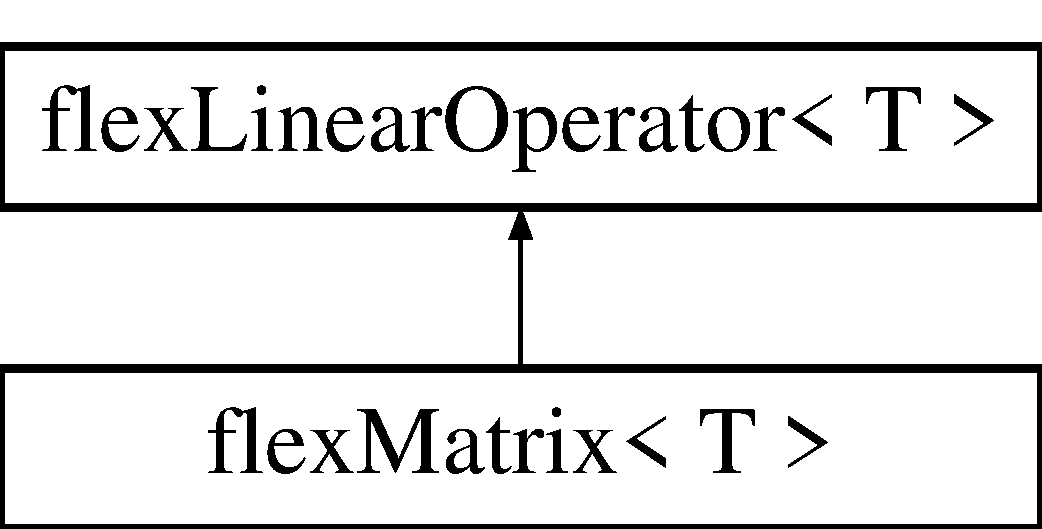
\includegraphics[height=2.000000cm]{classflex_matrix}
\end{center}
\end{figure}
\subsection*{Public Member Functions}
\begin{DoxyCompactItemize}
\item 
\mbox{\Hypertarget{classflex_matrix_a435c0b9173f4b27ae6a81f3fbfebc428}\label{classflex_matrix_a435c0b9173f4b27ae6a81f3fbfebc428}} 
\hyperlink{classflex_matrix_a435c0b9173f4b27ae6a81f3fbfebc428}{flex\+Matrix} ()
\begin{DoxyCompactList}\small\item\em initializes an empty matrix \end{DoxyCompactList}\item 
\hyperlink{classflex_matrix_a47ca204d9c79473c830e7582a7ff4e87}{flex\+Matrix} (int a\+Num\+Rows, int a\+Num\+Cols, bool a\+Minus)
\begin{DoxyCompactList}\small\item\em initializes a matrix \end{DoxyCompactList}\item 
\hyperlink{classflex_matrix}{flex\+Matrix}$<$ T $>$ $\ast$ \hyperlink{classflex_matrix_a4e9d53b8d606511759decbf52628203a}{copy} ()
\begin{DoxyCompactList}\small\item\em copies the linear operator \end{DoxyCompactList}\item 
void \hyperlink{classflex_matrix_ac7e95eed2025202b252d804034b923b6}{times} (bool transposed, const Tdata \&input, Tdata \&output)
\begin{DoxyCompactList}\small\item\em applies linear operator on vector \end{DoxyCompactList}\item 
void \hyperlink{classflex_matrix_a758c7520961d79e64bdf59d8ddb6bfb6}{times\+Plus} (bool transposed, const Tdata \&input, Tdata \&output)
\begin{DoxyCompactList}\small\item\em applies linear operator on vector and adds its result to y \end{DoxyCompactList}\item 
void \hyperlink{classflex_matrix_a100e59f7261d95eabc28fd9056d2b77b}{times\+Minus} (bool transposed, const Tdata \&input, Tdata \&output)
\begin{DoxyCompactList}\small\item\em applies linear operator on vector and substracts its result from y \end{DoxyCompactList}\item 
void \hyperlink{classflex_matrix_a028e2ab5d2ebbf2eec2e1a0c13e60421}{block\+Insert} (std\+::vector$<$ int $>$ \&indexI, const std\+::vector$<$ int $>$ \&indexJ, const Tdata \&index\+Val)
\begin{DoxyCompactList}\small\item\em inserts data into matrix \end{DoxyCompactList}\item 
T \hyperlink{classflex_matrix_a25cd9571e7056c4ad035a44a57e1d45d}{get\+Max\+Row\+Sum\+Abs} (bool transposed)
\begin{DoxyCompactList}\small\item\em returns the maximum sum of absolute values per row used for preconditioning \end{DoxyCompactList}\item 
std\+::vector$<$ T $>$ \hyperlink{classflex_matrix_a75f378787fc81ea2c570c9848a7f2588}{get\+Abs\+Row\+Sum} (bool transposed)
\begin{DoxyCompactList}\small\item\em returns a vector of sum of absolute values per row used for preconditioning \end{DoxyCompactList}\item 
void \hyperlink{classflex_matrix_aafd59b0c2f60fbff0df13fd3888f1cf3}{print\+Row} (int i)
\begin{DoxyCompactList}\small\item\em prints requested row \end{DoxyCompactList}\item 
\mbox{\Hypertarget{classflex_matrix_a25b466ea4ccd744b53cc13741b61cfc2}\label{classflex_matrix_a25b466ea4ccd744b53cc13741b61cfc2}} 
void \hyperlink{classflex_matrix_a25b466ea4ccd744b53cc13741b61cfc2}{print\+Matrix} ()
\begin{DoxyCompactList}\small\item\em prints the whole matrix \end{DoxyCompactList}\item 
thrust\+::device\+\_\+vector$<$ T $>$ \hyperlink{classflex_matrix_ae713d5dabcdab30df9b04f2a7d499235}{get\+Abs\+Row\+Sum\+C\+U\+DA} (bool transposed)
\begin{DoxyCompactList}\small\item\em same function as \hyperlink{classflex_matrix_a75f378787fc81ea2c570c9848a7f2588}{get\+Abs\+Row\+Sum()} but implemented in C\+U\+DA \end{DoxyCompactList}\end{DoxyCompactItemize}
\subsection*{Additional Inherited Members}


\subsection{Detailed Description}
\subsubsection*{template$<$typename T$>$\newline
class flex\+Matrix$<$ T $>$}

represents a (non-\/\+C\+U\+DA) matrix 

\subsection{Constructor \& Destructor Documentation}
\mbox{\Hypertarget{classflex_matrix_a47ca204d9c79473c830e7582a7ff4e87}\label{classflex_matrix_a47ca204d9c79473c830e7582a7ff4e87}} 
\index{flex\+Matrix@{flex\+Matrix}!flex\+Matrix@{flex\+Matrix}}
\index{flex\+Matrix@{flex\+Matrix}!flex\+Matrix@{flex\+Matrix}}
\subsubsection{\texorpdfstring{flex\+Matrix()}{flexMatrix()}}
{\footnotesize\ttfamily template$<$typename T$>$ \\
\hyperlink{classflex_matrix}{flex\+Matrix}$<$ T $>$\+::\hyperlink{classflex_matrix}{flex\+Matrix} (\begin{DoxyParamCaption}\item[{int}]{a\+Num\+Rows,  }\item[{int}]{a\+Num\+Cols,  }\item[{bool}]{a\+Minus }\end{DoxyParamCaption})\hspace{0.3cm}{\ttfamily [inline]}}



initializes a matrix 


\begin{DoxyParams}{Parameters}
{\em a\+Num\+Rows} & number of rows \\
\hline
{\em a\+Num\+Cols} & number of cols \\
\hline
{\em a\+Minus} & determines if operator is negated \\
\hline
\end{DoxyParams}
\begin{DoxySeeAlso}{See also}
\hyperlink{classflex_linear_operator_a7f986517e10aee21099ec7692b77905d}{is\+Minus} 
\end{DoxySeeAlso}


\subsection{Member Function Documentation}
\mbox{\Hypertarget{classflex_matrix_a028e2ab5d2ebbf2eec2e1a0c13e60421}\label{classflex_matrix_a028e2ab5d2ebbf2eec2e1a0c13e60421}} 
\index{flex\+Matrix@{flex\+Matrix}!block\+Insert@{block\+Insert}}
\index{block\+Insert@{block\+Insert}!flex\+Matrix@{flex\+Matrix}}
\subsubsection{\texorpdfstring{block\+Insert()}{blockInsert()}}
{\footnotesize\ttfamily template$<$typename T$>$ \\
void \hyperlink{classflex_matrix}{flex\+Matrix}$<$ T $>$\+::block\+Insert (\begin{DoxyParamCaption}\item[{std\+::vector$<$ int $>$ \&}]{indexI,  }\item[{const std\+::vector$<$ int $>$ \&}]{indexJ,  }\item[{const Tdata \&}]{index\+Val }\end{DoxyParamCaption})\hspace{0.3cm}{\ttfamily [inline]}}



inserts data into matrix 

this is the fastest way to fill \hyperlink{classflex_matrix}{flex\+Matrix} 
\begin{DoxyParams}{Parameters}
{\em indexI} & vector of row indices \\
\hline
{\em indexJ} & vector of column indices \\
\hline
{\em index\+Val} & vector of data corresponding row and column indices \\
\hline
\end{DoxyParams}
\mbox{\Hypertarget{classflex_matrix_a4e9d53b8d606511759decbf52628203a}\label{classflex_matrix_a4e9d53b8d606511759decbf52628203a}} 
\index{flex\+Matrix@{flex\+Matrix}!copy@{copy}}
\index{copy@{copy}!flex\+Matrix@{flex\+Matrix}}
\subsubsection{\texorpdfstring{copy()}{copy()}}
{\footnotesize\ttfamily template$<$typename T$>$ \\
\hyperlink{classflex_matrix}{flex\+Matrix}$<$T$>$$\ast$ \hyperlink{classflex_matrix}{flex\+Matrix}$<$ T $>$\+::copy (\begin{DoxyParamCaption}{ }\end{DoxyParamCaption})\hspace{0.3cm}{\ttfamily [inline]}, {\ttfamily [virtual]}}



copies the linear operator 

\begin{DoxyReturn}{Returns}
copy of linear operator 
\end{DoxyReturn}


Implements \hyperlink{classflex_linear_operator_a7cc1425677cc30fcbd092ffd28d508c9}{flex\+Linear\+Operator$<$ T $>$}.

\mbox{\Hypertarget{classflex_matrix_a75f378787fc81ea2c570c9848a7f2588}\label{classflex_matrix_a75f378787fc81ea2c570c9848a7f2588}} 
\index{flex\+Matrix@{flex\+Matrix}!get\+Abs\+Row\+Sum@{get\+Abs\+Row\+Sum}}
\index{get\+Abs\+Row\+Sum@{get\+Abs\+Row\+Sum}!flex\+Matrix@{flex\+Matrix}}
\subsubsection{\texorpdfstring{get\+Abs\+Row\+Sum()}{getAbsRowSum()}}
{\footnotesize\ttfamily template$<$typename T$>$ \\
std\+::vector$<$T$>$ \hyperlink{classflex_matrix}{flex\+Matrix}$<$ T $>$\+::get\+Abs\+Row\+Sum (\begin{DoxyParamCaption}\item[{bool}]{transposed }\end{DoxyParamCaption})\hspace{0.3cm}{\ttfamily [inline]}, {\ttfamily [virtual]}}



returns a vector of sum of absolute values per row used for preconditioning 


\begin{DoxyParams}{Parameters}
{\em transposed} & is true if operator should be (temporarily) transposed before usage \\
\hline
\end{DoxyParams}
\begin{DoxyReturn}{Returns}
vector of sum of absolute values per row 
\end{DoxyReturn}


Implements \hyperlink{classflex_linear_operator_ad6caa7b09e6e3c401cadef61b8e2307e}{flex\+Linear\+Operator$<$ T $>$}.

\mbox{\Hypertarget{classflex_matrix_ae713d5dabcdab30df9b04f2a7d499235}\label{classflex_matrix_ae713d5dabcdab30df9b04f2a7d499235}} 
\index{flex\+Matrix@{flex\+Matrix}!get\+Abs\+Row\+Sum\+C\+U\+DA@{get\+Abs\+Row\+Sum\+C\+U\+DA}}
\index{get\+Abs\+Row\+Sum\+C\+U\+DA@{get\+Abs\+Row\+Sum\+C\+U\+DA}!flex\+Matrix@{flex\+Matrix}}
\subsubsection{\texorpdfstring{get\+Abs\+Row\+Sum\+C\+U\+D\+A()}{getAbsRowSumCUDA()}}
{\footnotesize\ttfamily template$<$typename T$>$ \\
thrust\+::device\+\_\+vector$<$T$>$ \hyperlink{classflex_matrix}{flex\+Matrix}$<$ T $>$\+::get\+Abs\+Row\+Sum\+C\+U\+DA (\begin{DoxyParamCaption}\item[{bool}]{transposed }\end{DoxyParamCaption})\hspace{0.3cm}{\ttfamily [inline]}, {\ttfamily [virtual]}}



same function as \hyperlink{classflex_matrix_a75f378787fc81ea2c570c9848a7f2588}{get\+Abs\+Row\+Sum()} but implemented in C\+U\+DA 


\begin{DoxyParams}{Parameters}
{\em transposed} & is true if operator should be (temporarily) transposed before usage \\
\hline
\end{DoxyParams}
\begin{DoxyReturn}{Returns}
vector of sum of absolute values per row 
\end{DoxyReturn}


Implements \hyperlink{classflex_linear_operator_a0a0a431d43f4f9d36cbee0d31ba5a29b}{flex\+Linear\+Operator$<$ T $>$}.

\mbox{\Hypertarget{classflex_matrix_a25cd9571e7056c4ad035a44a57e1d45d}\label{classflex_matrix_a25cd9571e7056c4ad035a44a57e1d45d}} 
\index{flex\+Matrix@{flex\+Matrix}!get\+Max\+Row\+Sum\+Abs@{get\+Max\+Row\+Sum\+Abs}}
\index{get\+Max\+Row\+Sum\+Abs@{get\+Max\+Row\+Sum\+Abs}!flex\+Matrix@{flex\+Matrix}}
\subsubsection{\texorpdfstring{get\+Max\+Row\+Sum\+Abs()}{getMaxRowSumAbs()}}
{\footnotesize\ttfamily template$<$typename T$>$ \\
T \hyperlink{classflex_matrix}{flex\+Matrix}$<$ T $>$\+::get\+Max\+Row\+Sum\+Abs (\begin{DoxyParamCaption}\item[{bool}]{transposed }\end{DoxyParamCaption})\hspace{0.3cm}{\ttfamily [inline]}, {\ttfamily [virtual]}}



returns the maximum sum of absolute values per row used for preconditioning 


\begin{DoxyParams}{Parameters}
{\em transposed} & is true if operator should be (temporarily) transposed before usage \\
\hline
\end{DoxyParams}
\begin{DoxyReturn}{Returns}
maximum sum of absolute values per row 
\end{DoxyReturn}


Implements \hyperlink{classflex_linear_operator_afcb74697385ccb7c8d29870d7034c12a}{flex\+Linear\+Operator$<$ T $>$}.

\mbox{\Hypertarget{classflex_matrix_aafd59b0c2f60fbff0df13fd3888f1cf3}\label{classflex_matrix_aafd59b0c2f60fbff0df13fd3888f1cf3}} 
\index{flex\+Matrix@{flex\+Matrix}!print\+Row@{print\+Row}}
\index{print\+Row@{print\+Row}!flex\+Matrix@{flex\+Matrix}}
\subsubsection{\texorpdfstring{print\+Row()}{printRow()}}
{\footnotesize\ttfamily template$<$typename T$>$ \\
void \hyperlink{classflex_matrix}{flex\+Matrix}$<$ T $>$\+::print\+Row (\begin{DoxyParamCaption}\item[{int}]{i }\end{DoxyParamCaption})\hspace{0.3cm}{\ttfamily [inline]}}



prints requested row 


\begin{DoxyParams}{Parameters}
{\em i} & row to be printed \\
\hline
\end{DoxyParams}
\mbox{\Hypertarget{classflex_matrix_ac7e95eed2025202b252d804034b923b6}\label{classflex_matrix_ac7e95eed2025202b252d804034b923b6}} 
\index{flex\+Matrix@{flex\+Matrix}!times@{times}}
\index{times@{times}!flex\+Matrix@{flex\+Matrix}}
\subsubsection{\texorpdfstring{times()}{times()}}
{\footnotesize\ttfamily template$<$typename T$>$ \\
void \hyperlink{classflex_matrix}{flex\+Matrix}$<$ T $>$\+::times (\begin{DoxyParamCaption}\item[{bool}]{transposed,  }\item[{const Tdata \&}]{input,  }\item[{Tdata \&}]{output }\end{DoxyParamCaption})\hspace{0.3cm}{\ttfamily [inline]}, {\ttfamily [virtual]}}



applies linear operator on vector 

equals $ y = Ax $ 
\begin{DoxyParams}{Parameters}
{\em transposed} & is true if operator should be (temporarily) transposed before usage \\
\hline
{\em input} & data to be processed \\
\hline
{\em output} & output data \\
\hline
\end{DoxyParams}


Implements \hyperlink{classflex_linear_operator_a883982edf3be857815d2095e53f76e75}{flex\+Linear\+Operator$<$ T $>$}.

\mbox{\Hypertarget{classflex_matrix_a100e59f7261d95eabc28fd9056d2b77b}\label{classflex_matrix_a100e59f7261d95eabc28fd9056d2b77b}} 
\index{flex\+Matrix@{flex\+Matrix}!times\+Minus@{times\+Minus}}
\index{times\+Minus@{times\+Minus}!flex\+Matrix@{flex\+Matrix}}
\subsubsection{\texorpdfstring{times\+Minus()}{timesMinus()}}
{\footnotesize\ttfamily template$<$typename T$>$ \\
void \hyperlink{classflex_matrix}{flex\+Matrix}$<$ T $>$\+::times\+Minus (\begin{DoxyParamCaption}\item[{bool}]{transposed,  }\item[{const Tdata \&}]{input,  }\item[{Tdata \&}]{output }\end{DoxyParamCaption})\hspace{0.3cm}{\ttfamily [inline]}, {\ttfamily [virtual]}}



applies linear operator on vector and substracts its result from y 

equals $ y = y - Ax $ 
\begin{DoxyParams}{Parameters}
{\em transposed} & is true if operator should be (temporarily) transposed before usage \\
\hline
{\em input} & data to be processed \\
\hline
{\em output} & output data \\
\hline
\end{DoxyParams}


Implements \hyperlink{classflex_linear_operator_a62708874e134a649c8445df333079c69}{flex\+Linear\+Operator$<$ T $>$}.

\mbox{\Hypertarget{classflex_matrix_a758c7520961d79e64bdf59d8ddb6bfb6}\label{classflex_matrix_a758c7520961d79e64bdf59d8ddb6bfb6}} 
\index{flex\+Matrix@{flex\+Matrix}!times\+Plus@{times\+Plus}}
\index{times\+Plus@{times\+Plus}!flex\+Matrix@{flex\+Matrix}}
\subsubsection{\texorpdfstring{times\+Plus()}{timesPlus()}}
{\footnotesize\ttfamily template$<$typename T$>$ \\
void \hyperlink{classflex_matrix}{flex\+Matrix}$<$ T $>$\+::times\+Plus (\begin{DoxyParamCaption}\item[{bool}]{transposed,  }\item[{const Tdata \&}]{input,  }\item[{Tdata \&}]{output }\end{DoxyParamCaption})\hspace{0.3cm}{\ttfamily [inline]}, {\ttfamily [virtual]}}



applies linear operator on vector and adds its result to y 

equals $ y = y + Ax $ 
\begin{DoxyParams}{Parameters}
{\em transposed} & is true if operator should be (temporarily) transposed before usage \\
\hline
{\em input} & data to be processed \\
\hline
{\em output} & output data \\
\hline
\end{DoxyParams}


Implements \hyperlink{classflex_linear_operator_a3f2978ad1c5eae8cd4ae16deb2337416}{flex\+Linear\+Operator$<$ T $>$}.



The documentation for this class was generated from the following file\+:\begin{DoxyCompactItemize}
\item 
flex\+Matrix.\+h\end{DoxyCompactItemize}

\hypertarget{classflex_matrix_g_p_u}{}\section{flex\+Matrix\+G\+PU$<$ T $>$ Class Template Reference}
\label{classflex_matrix_g_p_u}\index{flex\+Matrix\+G\+P\+U$<$ T $>$@{flex\+Matrix\+G\+P\+U$<$ T $>$}}


represents a (C\+U\+DA) matrix  




{\ttfamily \#include $<$flex\+Matrix\+G\+P\+U.\+h$>$}

Inheritance diagram for flex\+Matrix\+G\+PU$<$ T $>$\+:\begin{figure}[H]
\begin{center}
\leavevmode
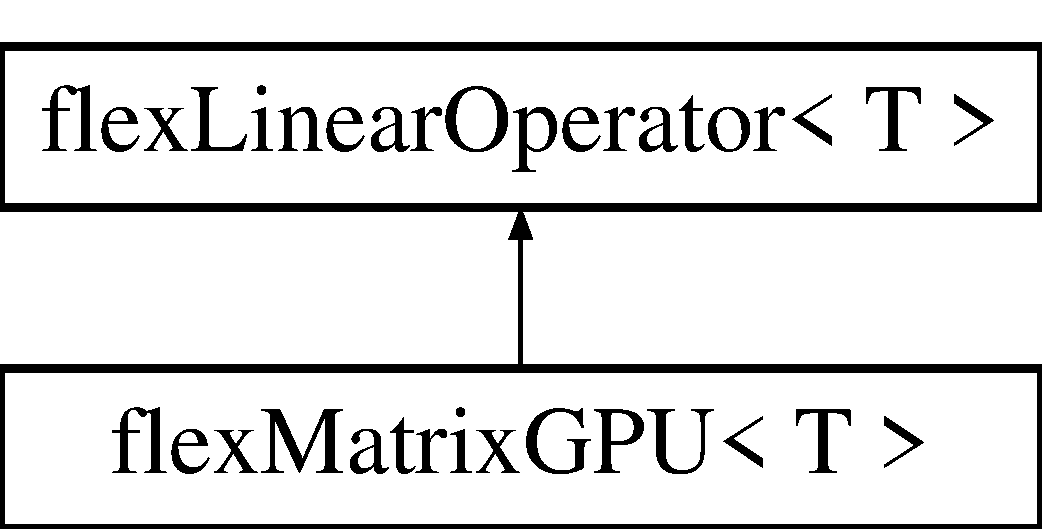
\includegraphics[height=2.000000cm]{classflex_matrix_g_p_u}
\end{center}
\end{figure}
\subsection*{Public Member Functions}
\begin{DoxyCompactItemize}
\item 
\hyperlink{classflex_matrix_g_p_u_a8fb0c0049604ddd6c51d39e1e96781f6}{flex\+Matrix\+G\+PU} (int a\+Num\+Rows, int a\+Num\+Cols, int $\ast$row\+List, int $\ast$col\+List, T $\ast$index\+Val, bool format\+C\+RS, bool a\+Minus)
\begin{DoxyCompactList}\small\item\em initializes a matrix \end{DoxyCompactList}\item 
\hyperlink{classflex_matrix_g_p_u}{flex\+Matrix\+G\+PU}$<$ T $>$ $\ast$ \hyperlink{classflex_matrix_g_p_u_a4df27ef284eec123ba72f1b5788f1180}{copy} ()
\begin{DoxyCompactList}\small\item\em copies the linear operator \end{DoxyCompactList}\item 
void \hyperlink{classflex_matrix_g_p_u_a059adf49cc4d895d017eed28462a29e4}{times} (bool transposed, const Tdata \&input, Tdata \&output)
\begin{DoxyCompactList}\small\item\em applies linear operator on vector \end{DoxyCompactList}\item 
void \hyperlink{classflex_matrix_g_p_u_adbb111427c3bc8ef6157ba60b3dbea3d}{times\+Plus} (bool transposed, const Tdata \&input, Tdata \&output)
\begin{DoxyCompactList}\small\item\em applies linear operator on vector and adds its result to y \end{DoxyCompactList}\item 
void \hyperlink{classflex_matrix_g_p_u_a4d6b328bba4170827a1ead228ecd8fcb}{times\+Minus} (bool transposed, const Tdata \&input, Tdata \&output)
\begin{DoxyCompactList}\small\item\em applies linear operator on vector and substracts its result from y \end{DoxyCompactList}\item 
T \hyperlink{classflex_matrix_g_p_u_aae4f81a403b6fff8ac73ccdf6c21399f}{get\+Max\+Row\+Sum\+Abs} (bool transposed)
\begin{DoxyCompactList}\small\item\em returns the maximum sum of absolute values per row used for preconditioning \end{DoxyCompactList}\item 
std\+::vector$<$ T $>$ \hyperlink{classflex_matrix_g_p_u_a0a1f19c482243223b8d98165d0b44ccf}{get\+Abs\+Row\+Sum} (bool transposed)
\begin{DoxyCompactList}\small\item\em returns a vector of sum of absolute values per row used for preconditioning \end{DoxyCompactList}\item 
void \hyperlink{classflex_matrix_g_p_u_a8de9cdb55021d3c25c56daf9a081d487}{print\+Row} (int i)
\begin{DoxyCompactList}\small\item\em prints requested row \end{DoxyCompactList}\item 
\mbox{\Hypertarget{classflex_matrix_g_p_u_a7717dbcb526b1a16f1a90a080880e42e}\label{classflex_matrix_g_p_u_a7717dbcb526b1a16f1a90a080880e42e}} 
void \hyperlink{classflex_matrix_g_p_u_a7717dbcb526b1a16f1a90a080880e42e}{print\+Matrix} ()
\begin{DoxyCompactList}\small\item\em prints the whole matrix \end{DoxyCompactList}\item 
thrust\+::device\+\_\+vector$<$ T $>$ \hyperlink{classflex_matrix_g_p_u_ab9fceb951d911794d4c70f5045255abd}{get\+Abs\+Row\+Sum\+C\+U\+DA} (bool transposed)
\begin{DoxyCompactList}\small\item\em same function as \hyperlink{classflex_matrix_g_p_u_a0a1f19c482243223b8d98165d0b44ccf}{get\+Abs\+Row\+Sum()} but implemented in C\+U\+DA \end{DoxyCompactList}\end{DoxyCompactItemize}
\subsection*{Additional Inherited Members}


\subsection{Detailed Description}
\subsubsection*{template$<$typename T$>$\newline
class flex\+Matrix\+G\+P\+U$<$ T $>$}

represents a (C\+U\+DA) matrix 

\subsection{Constructor \& Destructor Documentation}
\mbox{\Hypertarget{classflex_matrix_g_p_u_a8fb0c0049604ddd6c51d39e1e96781f6}\label{classflex_matrix_g_p_u_a8fb0c0049604ddd6c51d39e1e96781f6}} 
\index{flex\+Matrix\+G\+PU@{flex\+Matrix\+G\+PU}!flex\+Matrix\+G\+PU@{flex\+Matrix\+G\+PU}}
\index{flex\+Matrix\+G\+PU@{flex\+Matrix\+G\+PU}!flex\+Matrix\+G\+PU@{flex\+Matrix\+G\+PU}}
\subsubsection{\texorpdfstring{flex\+Matrix\+G\+P\+U()}{flexMatrixGPU()}}
{\footnotesize\ttfamily template$<$typename T$>$ \\
\hyperlink{classflex_matrix_g_p_u}{flex\+Matrix\+G\+PU}$<$ T $>$\+::\hyperlink{classflex_matrix_g_p_u}{flex\+Matrix\+G\+PU} (\begin{DoxyParamCaption}\item[{int}]{a\+Num\+Rows,  }\item[{int}]{a\+Num\+Cols,  }\item[{int $\ast$}]{row\+List,  }\item[{int $\ast$}]{col\+List,  }\item[{T $\ast$}]{index\+Val,  }\item[{bool}]{format\+C\+RS,  }\item[{bool}]{a\+Minus }\end{DoxyParamCaption})\hspace{0.3cm}{\ttfamily [inline]}}



initializes a matrix 


\begin{DoxyParams}{Parameters}
{\em a\+Num\+Rows} & number of rows \\
\hline
{\em a\+Num\+Cols} & number of cols \\
\hline
{\em row\+List} & array of row indices \\
\hline
{\em col\+List} & array of column indices \\
\hline
{\em index\+Val} & array of data corresponding row and column indices \\
\hline
{\em format\+C\+RS} & determines if the input data is in compressed row storage \\
\hline
{\em a\+Minus} & determines if operator is negated \\
\hline
\end{DoxyParams}
\begin{DoxySeeAlso}{See also}
\hyperlink{classflex_linear_operator_a7f986517e10aee21099ec7692b77905d}{is\+Minus} 
\end{DoxySeeAlso}


\subsection{Member Function Documentation}
\mbox{\Hypertarget{classflex_matrix_g_p_u_a4df27ef284eec123ba72f1b5788f1180}\label{classflex_matrix_g_p_u_a4df27ef284eec123ba72f1b5788f1180}} 
\index{flex\+Matrix\+G\+PU@{flex\+Matrix\+G\+PU}!copy@{copy}}
\index{copy@{copy}!flex\+Matrix\+G\+PU@{flex\+Matrix\+G\+PU}}
\subsubsection{\texorpdfstring{copy()}{copy()}}
{\footnotesize\ttfamily template$<$typename T$>$ \\
\hyperlink{classflex_matrix_g_p_u}{flex\+Matrix\+G\+PU}$<$T$>$$\ast$ \hyperlink{classflex_matrix_g_p_u}{flex\+Matrix\+G\+PU}$<$ T $>$\+::copy (\begin{DoxyParamCaption}{ }\end{DoxyParamCaption})\hspace{0.3cm}{\ttfamily [inline]}, {\ttfamily [virtual]}}



copies the linear operator 

\begin{DoxyReturn}{Returns}
copy of linear operator 
\end{DoxyReturn}


Implements \hyperlink{classflex_linear_operator_a7cc1425677cc30fcbd092ffd28d508c9}{flex\+Linear\+Operator$<$ T $>$}.

\mbox{\Hypertarget{classflex_matrix_g_p_u_a0a1f19c482243223b8d98165d0b44ccf}\label{classflex_matrix_g_p_u_a0a1f19c482243223b8d98165d0b44ccf}} 
\index{flex\+Matrix\+G\+PU@{flex\+Matrix\+G\+PU}!get\+Abs\+Row\+Sum@{get\+Abs\+Row\+Sum}}
\index{get\+Abs\+Row\+Sum@{get\+Abs\+Row\+Sum}!flex\+Matrix\+G\+PU@{flex\+Matrix\+G\+PU}}
\subsubsection{\texorpdfstring{get\+Abs\+Row\+Sum()}{getAbsRowSum()}}
{\footnotesize\ttfamily template$<$typename T$>$ \\
std\+::vector$<$T$>$ \hyperlink{classflex_matrix_g_p_u}{flex\+Matrix\+G\+PU}$<$ T $>$\+::get\+Abs\+Row\+Sum (\begin{DoxyParamCaption}\item[{bool}]{transposed }\end{DoxyParamCaption})\hspace{0.3cm}{\ttfamily [inline]}, {\ttfamily [virtual]}}



returns a vector of sum of absolute values per row used for preconditioning 


\begin{DoxyParams}{Parameters}
{\em transposed} & is true if operator should be (temporarily) transposed before usage \\
\hline
\end{DoxyParams}
\begin{DoxyReturn}{Returns}
vector of sum of absolute values per row 
\end{DoxyReturn}


Implements \hyperlink{classflex_linear_operator_ad6caa7b09e6e3c401cadef61b8e2307e}{flex\+Linear\+Operator$<$ T $>$}.

\mbox{\Hypertarget{classflex_matrix_g_p_u_ab9fceb951d911794d4c70f5045255abd}\label{classflex_matrix_g_p_u_ab9fceb951d911794d4c70f5045255abd}} 
\index{flex\+Matrix\+G\+PU@{flex\+Matrix\+G\+PU}!get\+Abs\+Row\+Sum\+C\+U\+DA@{get\+Abs\+Row\+Sum\+C\+U\+DA}}
\index{get\+Abs\+Row\+Sum\+C\+U\+DA@{get\+Abs\+Row\+Sum\+C\+U\+DA}!flex\+Matrix\+G\+PU@{flex\+Matrix\+G\+PU}}
\subsubsection{\texorpdfstring{get\+Abs\+Row\+Sum\+C\+U\+D\+A()}{getAbsRowSumCUDA()}}
{\footnotesize\ttfamily template$<$typename T$>$ \\
thrust\+::device\+\_\+vector$<$T$>$ \hyperlink{classflex_matrix_g_p_u}{flex\+Matrix\+G\+PU}$<$ T $>$\+::get\+Abs\+Row\+Sum\+C\+U\+DA (\begin{DoxyParamCaption}\item[{bool}]{transposed }\end{DoxyParamCaption})\hspace{0.3cm}{\ttfamily [inline]}, {\ttfamily [virtual]}}



same function as \hyperlink{classflex_matrix_g_p_u_a0a1f19c482243223b8d98165d0b44ccf}{get\+Abs\+Row\+Sum()} but implemented in C\+U\+DA 


\begin{DoxyParams}{Parameters}
{\em transposed} & is true if operator should be (temporarily) transposed before usage \\
\hline
\end{DoxyParams}
\begin{DoxyReturn}{Returns}
vector of sum of absolute values per row 
\end{DoxyReturn}


Implements \hyperlink{classflex_linear_operator_a0a0a431d43f4f9d36cbee0d31ba5a29b}{flex\+Linear\+Operator$<$ T $>$}.

\mbox{\Hypertarget{classflex_matrix_g_p_u_aae4f81a403b6fff8ac73ccdf6c21399f}\label{classflex_matrix_g_p_u_aae4f81a403b6fff8ac73ccdf6c21399f}} 
\index{flex\+Matrix\+G\+PU@{flex\+Matrix\+G\+PU}!get\+Max\+Row\+Sum\+Abs@{get\+Max\+Row\+Sum\+Abs}}
\index{get\+Max\+Row\+Sum\+Abs@{get\+Max\+Row\+Sum\+Abs}!flex\+Matrix\+G\+PU@{flex\+Matrix\+G\+PU}}
\subsubsection{\texorpdfstring{get\+Max\+Row\+Sum\+Abs()}{getMaxRowSumAbs()}}
{\footnotesize\ttfamily template$<$typename T$>$ \\
T \hyperlink{classflex_matrix_g_p_u}{flex\+Matrix\+G\+PU}$<$ T $>$\+::get\+Max\+Row\+Sum\+Abs (\begin{DoxyParamCaption}\item[{bool}]{transposed }\end{DoxyParamCaption})\hspace{0.3cm}{\ttfamily [inline]}, {\ttfamily [virtual]}}



returns the maximum sum of absolute values per row used for preconditioning 


\begin{DoxyParams}{Parameters}
{\em transposed} & is true if operator should be (temporarily) transposed before usage \\
\hline
\end{DoxyParams}
\begin{DoxyReturn}{Returns}
maximum sum of absolute values per row 
\end{DoxyReturn}


Implements \hyperlink{classflex_linear_operator_afcb74697385ccb7c8d29870d7034c12a}{flex\+Linear\+Operator$<$ T $>$}.

\mbox{\Hypertarget{classflex_matrix_g_p_u_a8de9cdb55021d3c25c56daf9a081d487}\label{classflex_matrix_g_p_u_a8de9cdb55021d3c25c56daf9a081d487}} 
\index{flex\+Matrix\+G\+PU@{flex\+Matrix\+G\+PU}!print\+Row@{print\+Row}}
\index{print\+Row@{print\+Row}!flex\+Matrix\+G\+PU@{flex\+Matrix\+G\+PU}}
\subsubsection{\texorpdfstring{print\+Row()}{printRow()}}
{\footnotesize\ttfamily template$<$typename T$>$ \\
void \hyperlink{classflex_matrix_g_p_u}{flex\+Matrix\+G\+PU}$<$ T $>$\+::print\+Row (\begin{DoxyParamCaption}\item[{int}]{i }\end{DoxyParamCaption})\hspace{0.3cm}{\ttfamily [inline]}}



prints requested row 


\begin{DoxyParams}{Parameters}
{\em i} & row to be printed \\
\hline
\end{DoxyParams}
\mbox{\Hypertarget{classflex_matrix_g_p_u_a059adf49cc4d895d017eed28462a29e4}\label{classflex_matrix_g_p_u_a059adf49cc4d895d017eed28462a29e4}} 
\index{flex\+Matrix\+G\+PU@{flex\+Matrix\+G\+PU}!times@{times}}
\index{times@{times}!flex\+Matrix\+G\+PU@{flex\+Matrix\+G\+PU}}
\subsubsection{\texorpdfstring{times()}{times()}}
{\footnotesize\ttfamily template$<$typename T$>$ \\
void \hyperlink{classflex_matrix_g_p_u}{flex\+Matrix\+G\+PU}$<$ T $>$\+::times (\begin{DoxyParamCaption}\item[{bool}]{transposed,  }\item[{const Tdata \&}]{input,  }\item[{Tdata \&}]{output }\end{DoxyParamCaption})\hspace{0.3cm}{\ttfamily [inline]}, {\ttfamily [virtual]}}



applies linear operator on vector 

equals $ y = Ax $ 
\begin{DoxyParams}{Parameters}
{\em transposed} & is true if operator should be (temporarily) transposed before usage \\
\hline
{\em input} & data to be processed \\
\hline
{\em output} & output data \\
\hline
\end{DoxyParams}


Implements \hyperlink{classflex_linear_operator_a883982edf3be857815d2095e53f76e75}{flex\+Linear\+Operator$<$ T $>$}.

\mbox{\Hypertarget{classflex_matrix_g_p_u_a4d6b328bba4170827a1ead228ecd8fcb}\label{classflex_matrix_g_p_u_a4d6b328bba4170827a1ead228ecd8fcb}} 
\index{flex\+Matrix\+G\+PU@{flex\+Matrix\+G\+PU}!times\+Minus@{times\+Minus}}
\index{times\+Minus@{times\+Minus}!flex\+Matrix\+G\+PU@{flex\+Matrix\+G\+PU}}
\subsubsection{\texorpdfstring{times\+Minus()}{timesMinus()}}
{\footnotesize\ttfamily template$<$typename T$>$ \\
void \hyperlink{classflex_matrix_g_p_u}{flex\+Matrix\+G\+PU}$<$ T $>$\+::times\+Minus (\begin{DoxyParamCaption}\item[{bool}]{transposed,  }\item[{const Tdata \&}]{input,  }\item[{Tdata \&}]{output }\end{DoxyParamCaption})\hspace{0.3cm}{\ttfamily [inline]}, {\ttfamily [virtual]}}



applies linear operator on vector and substracts its result from y 

equals $ y = y - Ax $ 
\begin{DoxyParams}{Parameters}
{\em transposed} & is true if operator should be (temporarily) transposed before usage \\
\hline
{\em input} & data to be processed \\
\hline
{\em output} & output data \\
\hline
\end{DoxyParams}


Implements \hyperlink{classflex_linear_operator_a62708874e134a649c8445df333079c69}{flex\+Linear\+Operator$<$ T $>$}.

\mbox{\Hypertarget{classflex_matrix_g_p_u_adbb111427c3bc8ef6157ba60b3dbea3d}\label{classflex_matrix_g_p_u_adbb111427c3bc8ef6157ba60b3dbea3d}} 
\index{flex\+Matrix\+G\+PU@{flex\+Matrix\+G\+PU}!times\+Plus@{times\+Plus}}
\index{times\+Plus@{times\+Plus}!flex\+Matrix\+G\+PU@{flex\+Matrix\+G\+PU}}
\subsubsection{\texorpdfstring{times\+Plus()}{timesPlus()}}
{\footnotesize\ttfamily template$<$typename T$>$ \\
void \hyperlink{classflex_matrix_g_p_u}{flex\+Matrix\+G\+PU}$<$ T $>$\+::times\+Plus (\begin{DoxyParamCaption}\item[{bool}]{transposed,  }\item[{const Tdata \&}]{input,  }\item[{Tdata \&}]{output }\end{DoxyParamCaption})\hspace{0.3cm}{\ttfamily [inline]}, {\ttfamily [virtual]}}



applies linear operator on vector and adds its result to y 

equals $ y = y + Ax $ 
\begin{DoxyParams}{Parameters}
{\em transposed} & is true if operator should be (temporarily) transposed before usage \\
\hline
{\em input} & data to be processed \\
\hline
{\em output} & output data \\
\hline
\end{DoxyParams}


Implements \hyperlink{classflex_linear_operator_a3f2978ad1c5eae8cd4ae16deb2337416}{flex\+Linear\+Operator$<$ T $>$}.



The documentation for this class was generated from the following file\+:\begin{DoxyCompactItemize}
\item 
flex\+Matrix\+G\+P\+U.\+h\end{DoxyCompactItemize}

\hypertarget{classflex_matrix_logical}{}\section{flex\+Matrix\+Logical$<$ T $>$ Class Template Reference}
\label{classflex_matrix_logical}\index{flex\+Matrix\+Logical$<$ T $>$@{flex\+Matrix\+Logical$<$ T $>$}}


represents a full (non-\/\+C\+U\+DA) logical matrix  




{\ttfamily \#include $<$flex\+Matrix\+Logical.\+h$>$}

Inheritance diagram for flex\+Matrix\+Logical$<$ T $>$\+:\begin{figure}[H]
\begin{center}
\leavevmode
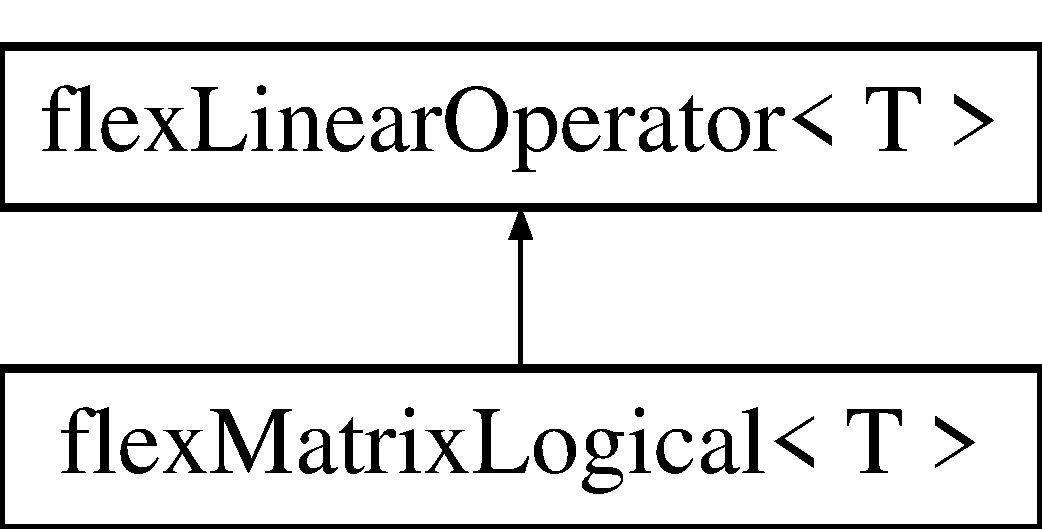
\includegraphics[height=2.000000cm]{classflex_matrix_logical}
\end{center}
\end{figure}
\subsection*{Public Member Functions}
\begin{DoxyCompactItemize}
\item 
\mbox{\Hypertarget{classflex_matrix_logical_a638c50a335498ef4f78d76f7304561f6}\label{classflex_matrix_logical_a638c50a335498ef4f78d76f7304561f6}} 
\hyperlink{classflex_matrix_logical_a638c50a335498ef4f78d76f7304561f6}{flex\+Matrix\+Logical} ()
\begin{DoxyCompactList}\small\item\em initializes an empty matrix \end{DoxyCompactList}\item 
\hyperlink{classflex_matrix_logical_abbd2d5d1be94e9d98167e82b6f0395be}{flex\+Matrix\+Logical} (int a\+Num\+Rows, int a\+Num\+Cols, bool a\+Minus)
\begin{DoxyCompactList}\small\item\em initializes a matrix \end{DoxyCompactList}\item 
\hyperlink{classflex_matrix_logical}{flex\+Matrix\+Logical}$<$ T $>$ $\ast$ \hyperlink{classflex_matrix_logical_a25c9ecc21cfccc07e1390c554784ee27}{copy} ()
\begin{DoxyCompactList}\small\item\em copies the linear operator \end{DoxyCompactList}\item 
void \hyperlink{classflex_matrix_logical_ab1ccf3400da547a27b5753a894905c63}{times} (bool transposed, const Tdata \&input, Tdata \&output)
\begin{DoxyCompactList}\small\item\em applies linear operator on vector \end{DoxyCompactList}\item 
void \hyperlink{classflex_matrix_logical_ad8a018f29237002d79faed523e5e2546}{times\+Plus} (bool transposed, const Tdata \&input, Tdata \&output)
\begin{DoxyCompactList}\small\item\em applies linear operator on vector and adds its result to y \end{DoxyCompactList}\item 
void \hyperlink{classflex_matrix_logical_a7f3b3d9f007696d7140c2f2256de8dd8}{times\+Minus} (bool transposed, const Tdata \&input, Tdata \&output)
\begin{DoxyCompactList}\small\item\em applies linear operator on vector and substracts its result from y \end{DoxyCompactList}\item 
void \hyperlink{classflex_matrix_logical_aea3347c0b215b0210ad5c100f32cea50}{block\+Insert} (const std\+::vector$<$ int $>$ \&indexI, const std\+::vector$<$ int $>$ \&indexJ)
\begin{DoxyCompactList}\small\item\em inserts position of all non-\/zero elements into matrix \end{DoxyCompactList}\item 
\mbox{\Hypertarget{classflex_matrix_logical_a613206c02ddb2de7d984258f307e664f}\label{classflex_matrix_logical_a613206c02ddb2de7d984258f307e664f}} 
int {\bfseries index2\+Dto\+Linear} (int i, int j)
\item 
T \hyperlink{classflex_matrix_logical_ab35a9ebf590236184573731bb08e176d}{get\+Max\+Row\+Sum\+Abs} (bool transposed)
\begin{DoxyCompactList}\small\item\em returns the maximum sum of absolute values per row used for preconditioning \end{DoxyCompactList}\item 
std\+::vector$<$ T $>$ \hyperlink{classflex_matrix_logical_a0c7cf2e5dde3a2d55ae95c6e54f94342}{get\+Abs\+Row\+Sum} (bool transposed)
\begin{DoxyCompactList}\small\item\em returns a vector of sum of absolute values per row used for preconditioning \end{DoxyCompactList}\item 
void \hyperlink{classflex_matrix_logical_a27805a561e6e94bdffe965dc8b9a3915}{print\+Row} (int i)
\begin{DoxyCompactList}\small\item\em prints requested row \end{DoxyCompactList}\item 
\mbox{\Hypertarget{classflex_matrix_logical_a36d592ff72cdd6d52268e3f0cbe38687}\label{classflex_matrix_logical_a36d592ff72cdd6d52268e3f0cbe38687}} 
void \hyperlink{classflex_matrix_logical_a36d592ff72cdd6d52268e3f0cbe38687}{print\+Matrix} ()
\begin{DoxyCompactList}\small\item\em prints the whole matrix \end{DoxyCompactList}\item 
thrust\+::device\+\_\+vector$<$ T $>$ \hyperlink{classflex_matrix_logical_a0245c73fb7d1fb3b1900208e0deb48d6}{get\+Abs\+Row\+Sum\+C\+U\+DA} (bool transposed)
\begin{DoxyCompactList}\small\item\em same function as \hyperlink{classflex_matrix_logical_a0c7cf2e5dde3a2d55ae95c6e54f94342}{get\+Abs\+Row\+Sum()} but implemented in C\+U\+DA \end{DoxyCompactList}\end{DoxyCompactItemize}
\subsection*{Public Attributes}
\begin{DoxyCompactItemize}
\item 
\mbox{\Hypertarget{classflex_matrix_logical_ae7b012bd8935f92c9e266f4a6d7ea91c}\label{classflex_matrix_logical_ae7b012bd8935f92c9e266f4a6d7ea91c}} 
std\+::vector$<$ int $>$ {\bfseries row\+To\+Index\+List}
\item 
\mbox{\Hypertarget{classflex_matrix_logical_aa8279c96a0b4f8f80db84b92faa763df}\label{classflex_matrix_logical_aa8279c96a0b4f8f80db84b92faa763df}} 
std\+::vector$<$ int $>$ {\bfseries index\+List}
\end{DoxyCompactItemize}


\subsection{Detailed Description}
\subsubsection*{template$<$typename T$>$\newline
class flex\+Matrix\+Logical$<$ T $>$}

represents a full (non-\/\+C\+U\+DA) logical matrix 

\subsection{Constructor \& Destructor Documentation}
\mbox{\Hypertarget{classflex_matrix_logical_abbd2d5d1be94e9d98167e82b6f0395be}\label{classflex_matrix_logical_abbd2d5d1be94e9d98167e82b6f0395be}} 
\index{flex\+Matrix\+Logical@{flex\+Matrix\+Logical}!flex\+Matrix\+Logical@{flex\+Matrix\+Logical}}
\index{flex\+Matrix\+Logical@{flex\+Matrix\+Logical}!flex\+Matrix\+Logical@{flex\+Matrix\+Logical}}
\subsubsection{\texorpdfstring{flex\+Matrix\+Logical()}{flexMatrixLogical()}}
{\footnotesize\ttfamily template$<$typename T$>$ \\
\hyperlink{classflex_matrix_logical}{flex\+Matrix\+Logical}$<$ T $>$\+::\hyperlink{classflex_matrix_logical}{flex\+Matrix\+Logical} (\begin{DoxyParamCaption}\item[{int}]{a\+Num\+Rows,  }\item[{int}]{a\+Num\+Cols,  }\item[{bool}]{a\+Minus }\end{DoxyParamCaption})\hspace{0.3cm}{\ttfamily [inline]}}



initializes a matrix 


\begin{DoxyParams}{Parameters}
{\em a\+Num\+Rows} & number of rows \\
\hline
{\em a\+Num\+Cols} & number of cols \\
\hline
{\em a\+Minus} & determines if operator is negated \\
\hline
\end{DoxyParams}
\begin{DoxySeeAlso}{See also}
\hyperlink{classflex_linear_operator_a7f986517e10aee21099ec7692b77905d}{is\+Minus} 
\end{DoxySeeAlso}


\subsection{Member Function Documentation}
\mbox{\Hypertarget{classflex_matrix_logical_aea3347c0b215b0210ad5c100f32cea50}\label{classflex_matrix_logical_aea3347c0b215b0210ad5c100f32cea50}} 
\index{flex\+Matrix\+Logical@{flex\+Matrix\+Logical}!block\+Insert@{block\+Insert}}
\index{block\+Insert@{block\+Insert}!flex\+Matrix\+Logical@{flex\+Matrix\+Logical}}
\subsubsection{\texorpdfstring{block\+Insert()}{blockInsert()}}
{\footnotesize\ttfamily template$<$typename T$>$ \\
void \hyperlink{classflex_matrix_logical}{flex\+Matrix\+Logical}$<$ T $>$\+::block\+Insert (\begin{DoxyParamCaption}\item[{const std\+::vector$<$ int $>$ \&}]{indexI,  }\item[{const std\+::vector$<$ int $>$ \&}]{indexJ }\end{DoxyParamCaption})\hspace{0.3cm}{\ttfamily [inline]}}



inserts position of all non-\/zero elements into matrix 

this is the fastest way to fill \hyperlink{classflex_matrix_logical}{flex\+Matrix\+Logical} 
\begin{DoxyParams}{Parameters}
{\em indexI} & vector of row indices \\
\hline
{\em indexJ} & vector of column indices \\
\hline
\end{DoxyParams}
\mbox{\Hypertarget{classflex_matrix_logical_a25c9ecc21cfccc07e1390c554784ee27}\label{classflex_matrix_logical_a25c9ecc21cfccc07e1390c554784ee27}} 
\index{flex\+Matrix\+Logical@{flex\+Matrix\+Logical}!copy@{copy}}
\index{copy@{copy}!flex\+Matrix\+Logical@{flex\+Matrix\+Logical}}
\subsubsection{\texorpdfstring{copy()}{copy()}}
{\footnotesize\ttfamily template$<$typename T$>$ \\
\hyperlink{classflex_matrix_logical}{flex\+Matrix\+Logical}$<$T$>$$\ast$ \hyperlink{classflex_matrix_logical}{flex\+Matrix\+Logical}$<$ T $>$\+::copy (\begin{DoxyParamCaption}{ }\end{DoxyParamCaption})\hspace{0.3cm}{\ttfamily [inline]}, {\ttfamily [virtual]}}



copies the linear operator 

\begin{DoxyReturn}{Returns}
copy of linear operator 
\end{DoxyReturn}


Implements \hyperlink{classflex_linear_operator_a7cc1425677cc30fcbd092ffd28d508c9}{flex\+Linear\+Operator$<$ T $>$}.

\mbox{\Hypertarget{classflex_matrix_logical_a0c7cf2e5dde3a2d55ae95c6e54f94342}\label{classflex_matrix_logical_a0c7cf2e5dde3a2d55ae95c6e54f94342}} 
\index{flex\+Matrix\+Logical@{flex\+Matrix\+Logical}!get\+Abs\+Row\+Sum@{get\+Abs\+Row\+Sum}}
\index{get\+Abs\+Row\+Sum@{get\+Abs\+Row\+Sum}!flex\+Matrix\+Logical@{flex\+Matrix\+Logical}}
\subsubsection{\texorpdfstring{get\+Abs\+Row\+Sum()}{getAbsRowSum()}}
{\footnotesize\ttfamily template$<$typename T$>$ \\
std\+::vector$<$T$>$ \hyperlink{classflex_matrix_logical}{flex\+Matrix\+Logical}$<$ T $>$\+::get\+Abs\+Row\+Sum (\begin{DoxyParamCaption}\item[{bool}]{transposed }\end{DoxyParamCaption})\hspace{0.3cm}{\ttfamily [inline]}, {\ttfamily [virtual]}}



returns a vector of sum of absolute values per row used for preconditioning 


\begin{DoxyParams}{Parameters}
{\em transposed} & is true if operator should be (temporarily) transposed before usage \\
\hline
\end{DoxyParams}
\begin{DoxyReturn}{Returns}
vector of sum of absolute values per row 
\end{DoxyReturn}


Implements \hyperlink{classflex_linear_operator_ad6caa7b09e6e3c401cadef61b8e2307e}{flex\+Linear\+Operator$<$ T $>$}.

\mbox{\Hypertarget{classflex_matrix_logical_a0245c73fb7d1fb3b1900208e0deb48d6}\label{classflex_matrix_logical_a0245c73fb7d1fb3b1900208e0deb48d6}} 
\index{flex\+Matrix\+Logical@{flex\+Matrix\+Logical}!get\+Abs\+Row\+Sum\+C\+U\+DA@{get\+Abs\+Row\+Sum\+C\+U\+DA}}
\index{get\+Abs\+Row\+Sum\+C\+U\+DA@{get\+Abs\+Row\+Sum\+C\+U\+DA}!flex\+Matrix\+Logical@{flex\+Matrix\+Logical}}
\subsubsection{\texorpdfstring{get\+Abs\+Row\+Sum\+C\+U\+D\+A()}{getAbsRowSumCUDA()}}
{\footnotesize\ttfamily template$<$typename T$>$ \\
thrust\+::device\+\_\+vector$<$T$>$ \hyperlink{classflex_matrix_logical}{flex\+Matrix\+Logical}$<$ T $>$\+::get\+Abs\+Row\+Sum\+C\+U\+DA (\begin{DoxyParamCaption}\item[{bool}]{transposed }\end{DoxyParamCaption})\hspace{0.3cm}{\ttfamily [inline]}, {\ttfamily [virtual]}}



same function as \hyperlink{classflex_matrix_logical_a0c7cf2e5dde3a2d55ae95c6e54f94342}{get\+Abs\+Row\+Sum()} but implemented in C\+U\+DA 


\begin{DoxyParams}{Parameters}
{\em transposed} & is true if operator should be (temporarily) transposed before usage \\
\hline
\end{DoxyParams}
\begin{DoxyReturn}{Returns}
vector of sum of absolute values per row 
\end{DoxyReturn}


Implements \hyperlink{classflex_linear_operator_a0a0a431d43f4f9d36cbee0d31ba5a29b}{flex\+Linear\+Operator$<$ T $>$}.

\mbox{\Hypertarget{classflex_matrix_logical_ab35a9ebf590236184573731bb08e176d}\label{classflex_matrix_logical_ab35a9ebf590236184573731bb08e176d}} 
\index{flex\+Matrix\+Logical@{flex\+Matrix\+Logical}!get\+Max\+Row\+Sum\+Abs@{get\+Max\+Row\+Sum\+Abs}}
\index{get\+Max\+Row\+Sum\+Abs@{get\+Max\+Row\+Sum\+Abs}!flex\+Matrix\+Logical@{flex\+Matrix\+Logical}}
\subsubsection{\texorpdfstring{get\+Max\+Row\+Sum\+Abs()}{getMaxRowSumAbs()}}
{\footnotesize\ttfamily template$<$typename T$>$ \\
T \hyperlink{classflex_matrix_logical}{flex\+Matrix\+Logical}$<$ T $>$\+::get\+Max\+Row\+Sum\+Abs (\begin{DoxyParamCaption}\item[{bool}]{transposed }\end{DoxyParamCaption})\hspace{0.3cm}{\ttfamily [inline]}, {\ttfamily [virtual]}}



returns the maximum sum of absolute values per row used for preconditioning 


\begin{DoxyParams}{Parameters}
{\em transposed} & is true if operator should be (temporarily) transposed before usage \\
\hline
\end{DoxyParams}
\begin{DoxyReturn}{Returns}
maximum sum of absolute values per row 
\end{DoxyReturn}


Implements \hyperlink{classflex_linear_operator_afcb74697385ccb7c8d29870d7034c12a}{flex\+Linear\+Operator$<$ T $>$}.

\mbox{\Hypertarget{classflex_matrix_logical_a27805a561e6e94bdffe965dc8b9a3915}\label{classflex_matrix_logical_a27805a561e6e94bdffe965dc8b9a3915}} 
\index{flex\+Matrix\+Logical@{flex\+Matrix\+Logical}!print\+Row@{print\+Row}}
\index{print\+Row@{print\+Row}!flex\+Matrix\+Logical@{flex\+Matrix\+Logical}}
\subsubsection{\texorpdfstring{print\+Row()}{printRow()}}
{\footnotesize\ttfamily template$<$typename T$>$ \\
void \hyperlink{classflex_matrix_logical}{flex\+Matrix\+Logical}$<$ T $>$\+::print\+Row (\begin{DoxyParamCaption}\item[{int}]{i }\end{DoxyParamCaption})\hspace{0.3cm}{\ttfamily [inline]}}



prints requested row 


\begin{DoxyParams}{Parameters}
{\em i} & row to be printed \\
\hline
\end{DoxyParams}
\mbox{\Hypertarget{classflex_matrix_logical_ab1ccf3400da547a27b5753a894905c63}\label{classflex_matrix_logical_ab1ccf3400da547a27b5753a894905c63}} 
\index{flex\+Matrix\+Logical@{flex\+Matrix\+Logical}!times@{times}}
\index{times@{times}!flex\+Matrix\+Logical@{flex\+Matrix\+Logical}}
\subsubsection{\texorpdfstring{times()}{times()}}
{\footnotesize\ttfamily template$<$typename T$>$ \\
void \hyperlink{classflex_matrix_logical}{flex\+Matrix\+Logical}$<$ T $>$\+::times (\begin{DoxyParamCaption}\item[{bool}]{transposed,  }\item[{const Tdata \&}]{input,  }\item[{Tdata \&}]{output }\end{DoxyParamCaption})\hspace{0.3cm}{\ttfamily [inline]}, {\ttfamily [virtual]}}



applies linear operator on vector 

equals $ y = Ax $ 
\begin{DoxyParams}{Parameters}
{\em transposed} & is true if operator should be (temporarily) transposed before usage \\
\hline
{\em input} & data to be processed \\
\hline
{\em output} & output data \\
\hline
\end{DoxyParams}


Implements \hyperlink{classflex_linear_operator_a883982edf3be857815d2095e53f76e75}{flex\+Linear\+Operator$<$ T $>$}.

\mbox{\Hypertarget{classflex_matrix_logical_a7f3b3d9f007696d7140c2f2256de8dd8}\label{classflex_matrix_logical_a7f3b3d9f007696d7140c2f2256de8dd8}} 
\index{flex\+Matrix\+Logical@{flex\+Matrix\+Logical}!times\+Minus@{times\+Minus}}
\index{times\+Minus@{times\+Minus}!flex\+Matrix\+Logical@{flex\+Matrix\+Logical}}
\subsubsection{\texorpdfstring{times\+Minus()}{timesMinus()}}
{\footnotesize\ttfamily template$<$typename T$>$ \\
void \hyperlink{classflex_matrix_logical}{flex\+Matrix\+Logical}$<$ T $>$\+::times\+Minus (\begin{DoxyParamCaption}\item[{bool}]{transposed,  }\item[{const Tdata \&}]{input,  }\item[{Tdata \&}]{output }\end{DoxyParamCaption})\hspace{0.3cm}{\ttfamily [inline]}, {\ttfamily [virtual]}}



applies linear operator on vector and substracts its result from y 

equals $ y = y - Ax $ 
\begin{DoxyParams}{Parameters}
{\em transposed} & is true if operator should be (temporarily) transposed before usage \\
\hline
{\em input} & data to be processed \\
\hline
{\em output} & output data \\
\hline
\end{DoxyParams}


Implements \hyperlink{classflex_linear_operator_a62708874e134a649c8445df333079c69}{flex\+Linear\+Operator$<$ T $>$}.

\mbox{\Hypertarget{classflex_matrix_logical_ad8a018f29237002d79faed523e5e2546}\label{classflex_matrix_logical_ad8a018f29237002d79faed523e5e2546}} 
\index{flex\+Matrix\+Logical@{flex\+Matrix\+Logical}!times\+Plus@{times\+Plus}}
\index{times\+Plus@{times\+Plus}!flex\+Matrix\+Logical@{flex\+Matrix\+Logical}}
\subsubsection{\texorpdfstring{times\+Plus()}{timesPlus()}}
{\footnotesize\ttfamily template$<$typename T$>$ \\
void \hyperlink{classflex_matrix_logical}{flex\+Matrix\+Logical}$<$ T $>$\+::times\+Plus (\begin{DoxyParamCaption}\item[{bool}]{transposed,  }\item[{const Tdata \&}]{input,  }\item[{Tdata \&}]{output }\end{DoxyParamCaption})\hspace{0.3cm}{\ttfamily [inline]}, {\ttfamily [virtual]}}



applies linear operator on vector and adds its result to y 

equals $ y = y + Ax $ 
\begin{DoxyParams}{Parameters}
{\em transposed} & is true if operator should be (temporarily) transposed before usage \\
\hline
{\em input} & data to be processed \\
\hline
{\em output} & output data \\
\hline
\end{DoxyParams}


Implements \hyperlink{classflex_linear_operator_a3f2978ad1c5eae8cd4ae16deb2337416}{flex\+Linear\+Operator$<$ T $>$}.



The documentation for this class was generated from the following file\+:\begin{DoxyCompactItemize}
\item 
flex\+Matrix\+Logical.\+h\end{DoxyCompactItemize}

\hypertarget{classflex_prox}{}\section{flex\+Prox$<$ T $>$ Class Template Reference}
\label{classflex_prox}\index{flex\+Prox$<$ T $>$@{flex\+Prox$<$ T $>$}}


abstract base class for all proximals (prox)  




{\ttfamily \#include $<$flex\+Prox.\+h$>$}

Inheritance diagram for flex\+Prox$<$ T $>$\+:\begin{figure}[H]
\begin{center}
\leavevmode
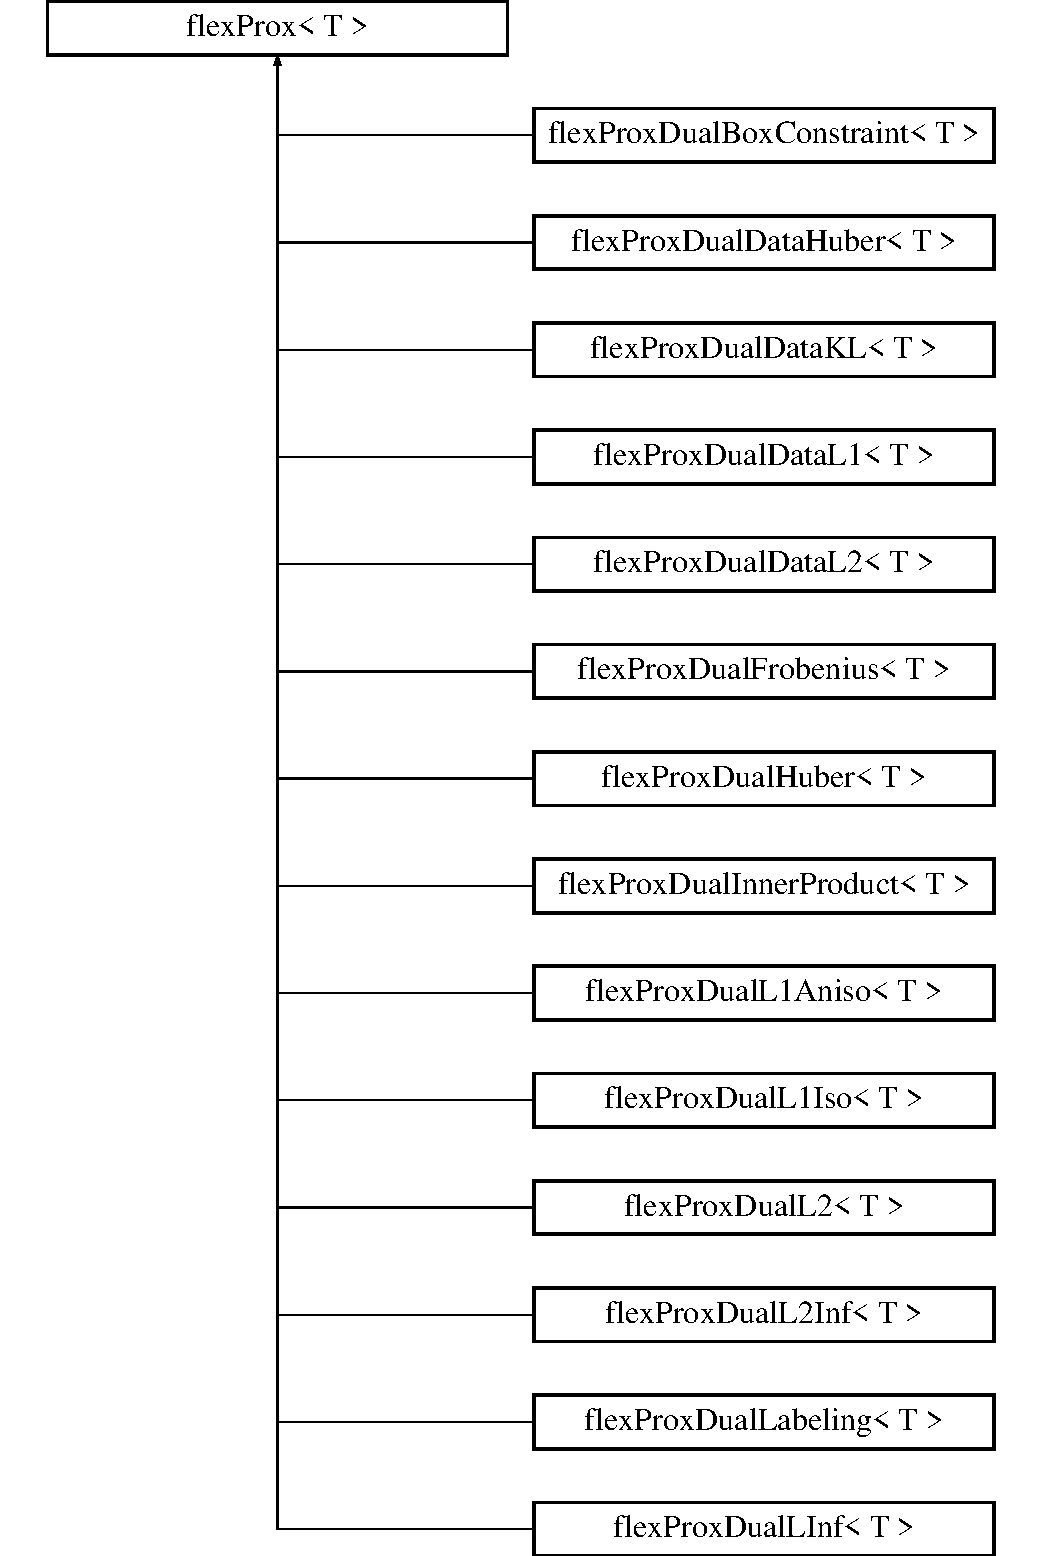
\includegraphics[height=12.000000cm]{classflex_prox}
\end{center}
\end{figure}
\subsection*{Public Member Functions}
\begin{DoxyCompactItemize}
\item 
\hyperlink{classflex_prox_a6055dee6acc0a2eedebf11c6ee4b644b}{flex\+Prox} (\hyperlink{tools_8h_aa34fd4f0962337a24e898ac0abdfff22}{prox} aP)
\begin{DoxyCompactList}\small\item\em initializes the prox \end{DoxyCompactList}\item 
\hyperlink{tools_8h_aa34fd4f0962337a24e898ac0abdfff22}{prox} \hyperlink{classflex_prox_a86e900bae3979620dcc6de3a5da89c8e}{get\+Prox} ()
\begin{DoxyCompactList}\small\item\em returns the type of prox \end{DoxyCompactList}\item 
virtual void \hyperlink{classflex_prox_a6d3119bd368c4216ad264a1f6dc1d01f}{apply\+Prox} (T alpha, \hyperlink{classflex_box_data}{flex\+Box\+Data}$<$ T $>$ $\ast$data, const std\+::vector$<$ int $>$ \&dual\+Numbers, const std\+::vector$<$ int $>$ \&primal\+Numbers)=0
\begin{DoxyCompactList}\small\item\em applies prox for non-\/data terms \end{DoxyCompactList}\item 
virtual void \hyperlink{classflex_prox_aec433ffbf1a7586f26a2116c6b94bdd6}{apply\+Prox} (T alpha, \hyperlink{classflex_box_data}{flex\+Box\+Data}$<$ T $>$ $\ast$data, const std\+::vector$<$ int $>$ \&dual\+Numbers, const std\+::vector$<$ int $>$ \&primal\+Numbers, std\+::vector$<$ Tdata $>$ \&f\+List)=0
\begin{DoxyCompactList}\small\item\em applies prox for data terms \end{DoxyCompactList}\end{DoxyCompactItemize}
\subsection*{Public Attributes}
\begin{DoxyCompactItemize}
\item 
const \hyperlink{tools_8h_aa34fd4f0962337a24e898ac0abdfff22}{prox} \hyperlink{classflex_prox_a5e62beeddd95e33d0a55319a05f44855}{p}
\begin{DoxyCompactList}\small\item\em type of prox \end{DoxyCompactList}\end{DoxyCompactItemize}


\subsection{Detailed Description}
\subsubsection*{template$<$typename T$>$\newline
class flex\+Prox$<$ T $>$}

abstract base class for all proximals (prox) 

\hyperlink{classflex_prox}{flex\+Prox} combines the interface for all usable proximals (prox) 

\subsection{Constructor \& Destructor Documentation}
\mbox{\Hypertarget{classflex_prox_a6055dee6acc0a2eedebf11c6ee4b644b}\label{classflex_prox_a6055dee6acc0a2eedebf11c6ee4b644b}} 
\index{flex\+Prox@{flex\+Prox}!flex\+Prox@{flex\+Prox}}
\index{flex\+Prox@{flex\+Prox}!flex\+Prox@{flex\+Prox}}
\subsubsection{\texorpdfstring{flex\+Prox()}{flexProx()}}
{\footnotesize\ttfamily template$<$typename T$>$ \\
\hyperlink{classflex_prox}{flex\+Prox}$<$ T $>$\+::\hyperlink{classflex_prox}{flex\+Prox} (\begin{DoxyParamCaption}\item[{\hyperlink{tools_8h_aa34fd4f0962337a24e898ac0abdfff22}{prox}}]{aP }\end{DoxyParamCaption})\hspace{0.3cm}{\ttfamily [inline]}}



initializes the prox 


\begin{DoxyParams}{Parameters}
{\em aP} & type of prox \\
\hline
\end{DoxyParams}


\subsection{Member Function Documentation}
\mbox{\Hypertarget{classflex_prox_a6d3119bd368c4216ad264a1f6dc1d01f}\label{classflex_prox_a6d3119bd368c4216ad264a1f6dc1d01f}} 
\index{flex\+Prox@{flex\+Prox}!apply\+Prox@{apply\+Prox}}
\index{apply\+Prox@{apply\+Prox}!flex\+Prox@{flex\+Prox}}
\subsubsection{\texorpdfstring{apply\+Prox()}{applyProx()}\hspace{0.1cm}{\footnotesize\ttfamily [1/2]}}
{\footnotesize\ttfamily template$<$typename T$>$ \\
virtual void \hyperlink{classflex_prox}{flex\+Prox}$<$ T $>$\+::apply\+Prox (\begin{DoxyParamCaption}\item[{T}]{alpha,  }\item[{\hyperlink{classflex_box_data}{flex\+Box\+Data}$<$ T $>$ $\ast$}]{data,  }\item[{const std\+::vector$<$ int $>$ \&}]{dual\+Numbers,  }\item[{const std\+::vector$<$ int $>$ \&}]{primal\+Numbers }\end{DoxyParamCaption})\hspace{0.3cm}{\ttfamily [pure virtual]}}



applies prox for non-\/data terms 

the function body should be empty if implemented prox is a data prox 
\begin{DoxyParams}{Parameters}
{\em alpha} & weight of term \\
\hline
{\em data} & data object \\
\hline
{\em dual\+Numbers} & vector of internal identifactions of dual numbers corresponding to the term \\
\hline
\end{DoxyParams}
\begin{DoxySeeAlso}{See also}
\hyperlink{classflex_box}{flex\+Box} 
\end{DoxySeeAlso}

\begin{DoxyParams}{Parameters}
{\em primal\+Numbers} & vector of internal identifactions of primal numbers corresponding to the term \\
\hline
\end{DoxyParams}
\begin{DoxySeeAlso}{See also}
\hyperlink{classflex_box}{flex\+Box} 
\end{DoxySeeAlso}


Implemented in \hyperlink{classflex_prox_dual_labeling_a29e89f413ea586b9390da273141c823b}{flex\+Prox\+Dual\+Labeling$<$ T $>$}, \hyperlink{classflex_prox_dual_l2_inf_a9462624e3c2cf958ea396b18d1773f9a}{flex\+Prox\+Dual\+L2\+Inf$<$ T $>$}, \hyperlink{classflex_prox_dual_l_inf_a90e3ad5244d8bf6cef50541593fb9da0}{flex\+Prox\+Dual\+L\+Inf$<$ T $>$}, \hyperlink{classflex_prox_dual_huber_af1e80a4361cda51e2b51aceeb69c6b79}{flex\+Prox\+Dual\+Huber$<$ T $>$}, \hyperlink{classflex_prox_dual_l1_iso_afbf9d355a5c633355233f6b7d6026465}{flex\+Prox\+Dual\+L1\+Iso$<$ T $>$}, \hyperlink{classflex_prox_dual_frobenius_a08de45a25d007ea87379641d027fd228}{flex\+Prox\+Dual\+Frobenius$<$ T $>$}, \hyperlink{classflex_prox_dual_box_constraint_a53df35f535f7df3da4e24f6190be2f7f}{flex\+Prox\+Dual\+Box\+Constraint$<$ T $>$}, \hyperlink{classflex_prox_dual_data_huber_ac085f34619c3d747b09a2b369a11dcd5}{flex\+Prox\+Dual\+Data\+Huber$<$ T $>$}, \hyperlink{classflex_prox_dual_data_l1_a8ebb08fae14a70bc6ed15b6d75b67705}{flex\+Prox\+Dual\+Data\+L1$<$ T $>$}, \hyperlink{classflex_prox_dual_l2_ad4574da3855bad6596c8a3fda028c933}{flex\+Prox\+Dual\+L2$<$ T $>$}, \hyperlink{classflex_prox_dual_l1_aniso_afef01f75247ba5a8990c5b77a7ab89f0}{flex\+Prox\+Dual\+L1\+Aniso$<$ T $>$}, \hyperlink{classflex_prox_dual_inner_product_ac12298c520f5e8e81724e330e8dae6a3}{flex\+Prox\+Dual\+Inner\+Product$<$ T $>$}, \hyperlink{classflex_prox_dual_data_k_l_ad6314cbdf307759e3176e26b3efba7c6}{flex\+Prox\+Dual\+Data\+K\+L$<$ T $>$}, and \hyperlink{classflex_prox_dual_data_l2_ae3ee176dc6c05e8fba0df96c73b10464}{flex\+Prox\+Dual\+Data\+L2$<$ T $>$}.

\mbox{\Hypertarget{classflex_prox_aec433ffbf1a7586f26a2116c6b94bdd6}\label{classflex_prox_aec433ffbf1a7586f26a2116c6b94bdd6}} 
\index{flex\+Prox@{flex\+Prox}!apply\+Prox@{apply\+Prox}}
\index{apply\+Prox@{apply\+Prox}!flex\+Prox@{flex\+Prox}}
\subsubsection{\texorpdfstring{apply\+Prox()}{applyProx()}\hspace{0.1cm}{\footnotesize\ttfamily [2/2]}}
{\footnotesize\ttfamily template$<$typename T$>$ \\
virtual void \hyperlink{classflex_prox}{flex\+Prox}$<$ T $>$\+::apply\+Prox (\begin{DoxyParamCaption}\item[{T}]{alpha,  }\item[{\hyperlink{classflex_box_data}{flex\+Box\+Data}$<$ T $>$ $\ast$}]{data,  }\item[{const std\+::vector$<$ int $>$ \&}]{dual\+Numbers,  }\item[{const std\+::vector$<$ int $>$ \&}]{primal\+Numbers,  }\item[{std\+::vector$<$ Tdata $>$ \&}]{f\+List }\end{DoxyParamCaption})\hspace{0.3cm}{\ttfamily [pure virtual]}}



applies prox for data terms 

the function body should be empty if implemented prox is a non-\/data prox 
\begin{DoxyParams}{Parameters}
{\em alpha} & weight of term \\
\hline
{\em data} & data object \\
\hline
{\em dual\+Numbers} & vector of internal identifactions of dual numbers corresponding to the term \\
\hline
\end{DoxyParams}
\begin{DoxySeeAlso}{See also}
\hyperlink{classflex_box}{flex\+Box} 
\end{DoxySeeAlso}

\begin{DoxyParams}{Parameters}
{\em primal\+Numbers} & vector of internal identifactions of primal numbers corresponding to the term \\
\hline
\end{DoxyParams}
\begin{DoxySeeAlso}{See also}
\hyperlink{classflex_box}{flex\+Box} 
\end{DoxySeeAlso}

\begin{DoxyParams}{Parameters}
{\em f\+List} & data part of term \\
\hline
\end{DoxyParams}


Implemented in \hyperlink{classflex_prox_dual_l2_inf_a01510c0adf9e21804b4ab93e728238e6}{flex\+Prox\+Dual\+L2\+Inf$<$ T $>$}, \hyperlink{classflex_prox_dual_huber_a4ce1a386510236fb80213dec59430ac4}{flex\+Prox\+Dual\+Huber$<$ T $>$}, \hyperlink{classflex_prox_dual_l_inf_a3ead6ede3f9535c5540c91955f83313b}{flex\+Prox\+Dual\+L\+Inf$<$ T $>$}, \hyperlink{classflex_prox_dual_l1_iso_a5cd236c5d3e58b9424b1021694c44590}{flex\+Prox\+Dual\+L1\+Iso$<$ T $>$}, \hyperlink{classflex_prox_dual_frobenius_a24695ced8a80693606e1654b04bd068f}{flex\+Prox\+Dual\+Frobenius$<$ T $>$}, \hyperlink{classflex_prox_dual_labeling_a224460146ef61af8b939e4a961cbe776}{flex\+Prox\+Dual\+Labeling$<$ T $>$}, \hyperlink{classflex_prox_dual_box_constraint_a417cfa67f4bffbfc102de872a3456990}{flex\+Prox\+Dual\+Box\+Constraint$<$ T $>$}, \hyperlink{classflex_prox_dual_l2_aef49de69c4d5e6baafbecbab934c17ce}{flex\+Prox\+Dual\+L2$<$ T $>$}, \hyperlink{classflex_prox_dual_l1_aniso_aff8e46fb892387898d54516f0df3c080}{flex\+Prox\+Dual\+L1\+Aniso$<$ T $>$}, \hyperlink{classflex_prox_dual_data_huber_ab1c0bbd454ee7fe65592ff8beda4aaa5}{flex\+Prox\+Dual\+Data\+Huber$<$ T $>$}, \hyperlink{classflex_prox_dual_data_k_l_aa02947fd71697cdb7d6d7e0d617fdfc3}{flex\+Prox\+Dual\+Data\+K\+L$<$ T $>$}, \hyperlink{classflex_prox_dual_data_l1_a3487ee84a12852486a1639d3b9dea735}{flex\+Prox\+Dual\+Data\+L1$<$ T $>$}, \hyperlink{classflex_prox_dual_data_l2_a0d7a54201b01863a9a76f6fc2d52cf22}{flex\+Prox\+Dual\+Data\+L2$<$ T $>$}, and \hyperlink{classflex_prox_dual_inner_product_aa2444bfc4ad1c4ce77e9204bd9f85f69}{flex\+Prox\+Dual\+Inner\+Product$<$ T $>$}.

\mbox{\Hypertarget{classflex_prox_a86e900bae3979620dcc6de3a5da89c8e}\label{classflex_prox_a86e900bae3979620dcc6de3a5da89c8e}} 
\index{flex\+Prox@{flex\+Prox}!get\+Prox@{get\+Prox}}
\index{get\+Prox@{get\+Prox}!flex\+Prox@{flex\+Prox}}
\subsubsection{\texorpdfstring{get\+Prox()}{getProx()}}
{\footnotesize\ttfamily template$<$typename T$>$ \\
\hyperlink{tools_8h_aa34fd4f0962337a24e898ac0abdfff22}{prox} \hyperlink{classflex_prox}{flex\+Prox}$<$ T $>$\+::get\+Prox (\begin{DoxyParamCaption}{ }\end{DoxyParamCaption})\hspace{0.3cm}{\ttfamily [inline]}}



returns the type of prox 

\begin{DoxyReturn}{Returns}
type of prox 
\end{DoxyReturn}


\subsection{Member Data Documentation}
\mbox{\Hypertarget{classflex_prox_a5e62beeddd95e33d0a55319a05f44855}\label{classflex_prox_a5e62beeddd95e33d0a55319a05f44855}} 
\index{flex\+Prox@{flex\+Prox}!p@{p}}
\index{p@{p}!flex\+Prox@{flex\+Prox}}
\subsubsection{\texorpdfstring{p}{p}}
{\footnotesize\ttfamily template$<$typename T$>$ \\
const \hyperlink{tools_8h_aa34fd4f0962337a24e898ac0abdfff22}{prox} \hyperlink{classflex_prox}{flex\+Prox}$<$ T $>$\+::p}



type of prox 

\begin{DoxySeeAlso}{See also}
\hyperlink{tools_8h_aa34fd4f0962337a24e898ac0abdfff22}{prox} 
\end{DoxySeeAlso}


The documentation for this class was generated from the following file\+:\begin{DoxyCompactItemize}
\item 
flex\+Prox.\+h\end{DoxyCompactItemize}

\hypertarget{classflex_prox_dual_box_constraint}{}\section{flex\+Prox\+Dual\+Box\+Constraint$<$ T $>$ Class Template Reference}
\label{classflex_prox_dual_box_constraint}\index{flex\+Prox\+Dual\+Box\+Constraint$<$ T $>$@{flex\+Prox\+Dual\+Box\+Constraint$<$ T $>$}}


represents prox for a box constraint  




{\ttfamily \#include $<$flex\+Prox\+Dual\+Box\+Constraint.\+h$>$}

Inheritance diagram for flex\+Prox\+Dual\+Box\+Constraint$<$ T $>$\+:\begin{figure}[H]
\begin{center}
\leavevmode
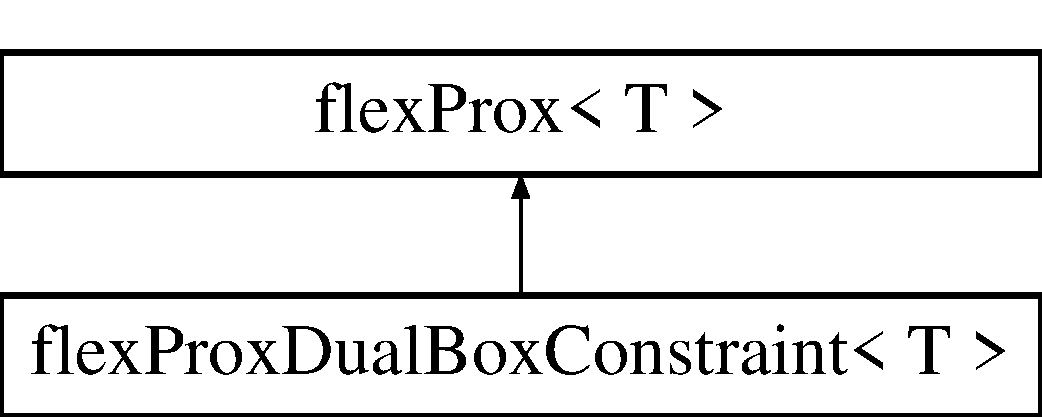
\includegraphics[height=2.000000cm]{classflex_prox_dual_box_constraint}
\end{center}
\end{figure}
\subsection*{Classes}
\begin{DoxyCompactItemize}
\item 
struct {\bfseries flex\+Prox\+Dual\+Box\+Constraint\+Functor}
\end{DoxyCompactItemize}
\subsection*{Public Member Functions}
\begin{DoxyCompactItemize}
\item 
\hyperlink{classflex_prox_dual_box_constraint_a2654a4ed37ad0eba9e6808f2a72ea1b3}{flex\+Prox\+Dual\+Box\+Constraint} (T a\+Min\+Val, T a\+Max\+Val)
\begin{DoxyCompactList}\small\item\em initializes the box constraint prox \end{DoxyCompactList}\item 
void \hyperlink{classflex_prox_dual_box_constraint_a53df35f535f7df3da4e24f6190be2f7f}{apply\+Prox} (T alpha, \hyperlink{classflex_box_data}{flex\+Box\+Data}$<$ T $>$ $\ast$data, const std\+::vector$<$ int $>$ \&dual\+Numbers, const std\+::vector$<$ int $>$ \&primal\+Numbers)
\begin{DoxyCompactList}\small\item\em applies prox for non-\/data terms \end{DoxyCompactList}\item 
void \hyperlink{classflex_prox_dual_box_constraint_a417cfa67f4bffbfc102de872a3456990}{apply\+Prox} (T alpha, \hyperlink{classflex_box_data}{flex\+Box\+Data}$<$ T $>$ $\ast$data, const std\+::vector$<$ int $>$ \&dual\+Numbers, const std\+::vector$<$ int $>$ \&primal\+Numbers, std\+::vector$<$ Tdata $>$ \&f\+List)
\begin{DoxyCompactList}\small\item\em applies prox for data terms \end{DoxyCompactList}\end{DoxyCompactItemize}
\subsection*{Additional Inherited Members}


\subsection{Detailed Description}
\subsubsection*{template$<$typename T$>$\newline
class flex\+Prox\+Dual\+Box\+Constraint$<$ T $>$}

represents prox for a box constraint 

$ \delta_{\{\bar{u} : u_{1}\leq \bar{u}\leq u_{2} \}}(\cdot) $ 

\subsection{Constructor \& Destructor Documentation}
\mbox{\Hypertarget{classflex_prox_dual_box_constraint_a2654a4ed37ad0eba9e6808f2a72ea1b3}\label{classflex_prox_dual_box_constraint_a2654a4ed37ad0eba9e6808f2a72ea1b3}} 
\index{flex\+Prox\+Dual\+Box\+Constraint@{flex\+Prox\+Dual\+Box\+Constraint}!flex\+Prox\+Dual\+Box\+Constraint@{flex\+Prox\+Dual\+Box\+Constraint}}
\index{flex\+Prox\+Dual\+Box\+Constraint@{flex\+Prox\+Dual\+Box\+Constraint}!flex\+Prox\+Dual\+Box\+Constraint@{flex\+Prox\+Dual\+Box\+Constraint}}
\subsubsection{\texorpdfstring{flex\+Prox\+Dual\+Box\+Constraint()}{flexProxDualBoxConstraint()}}
{\footnotesize\ttfamily template$<$typename T $>$ \\
\hyperlink{classflex_prox_dual_box_constraint}{flex\+Prox\+Dual\+Box\+Constraint}$<$ T $>$\+::\hyperlink{classflex_prox_dual_box_constraint}{flex\+Prox\+Dual\+Box\+Constraint} (\begin{DoxyParamCaption}\item[{T}]{a\+Min\+Val,  }\item[{T}]{a\+Max\+Val }\end{DoxyParamCaption})\hspace{0.3cm}{\ttfamily [inline]}}



initializes the box constraint prox 


\begin{DoxyParams}{Parameters}
{\em a\+Minval} & lower bound (equals $u_1$) \\
\hline
{\em a\+Max\+Val} & upper bound (equals $u_2$) \\
\hline
\end{DoxyParams}


\subsection{Member Function Documentation}
\mbox{\Hypertarget{classflex_prox_dual_box_constraint_a53df35f535f7df3da4e24f6190be2f7f}\label{classflex_prox_dual_box_constraint_a53df35f535f7df3da4e24f6190be2f7f}} 
\index{flex\+Prox\+Dual\+Box\+Constraint@{flex\+Prox\+Dual\+Box\+Constraint}!apply\+Prox@{apply\+Prox}}
\index{apply\+Prox@{apply\+Prox}!flex\+Prox\+Dual\+Box\+Constraint@{flex\+Prox\+Dual\+Box\+Constraint}}
\subsubsection{\texorpdfstring{apply\+Prox()}{applyProx()}\hspace{0.1cm}{\footnotesize\ttfamily [1/2]}}
{\footnotesize\ttfamily template$<$typename T $>$ \\
void \hyperlink{classflex_prox_dual_box_constraint}{flex\+Prox\+Dual\+Box\+Constraint}$<$ T $>$\+::apply\+Prox (\begin{DoxyParamCaption}\item[{T}]{alpha,  }\item[{\hyperlink{classflex_box_data}{flex\+Box\+Data}$<$ T $>$ $\ast$}]{data,  }\item[{const std\+::vector$<$ int $>$ \&}]{dual\+Numbers,  }\item[{const std\+::vector$<$ int $>$ \&}]{primal\+Numbers }\end{DoxyParamCaption})\hspace{0.3cm}{\ttfamily [inline]}, {\ttfamily [virtual]}}



applies prox for non-\/data terms 

the function body should be empty if implemented prox is a data prox 
\begin{DoxyParams}{Parameters}
{\em alpha} & weight of term \\
\hline
{\em data} & data object \\
\hline
{\em dual\+Numbers} & vector of internal identifactions of dual numbers corresponding to the term \\
\hline
\end{DoxyParams}
\begin{DoxySeeAlso}{See also}
\hyperlink{classflex_box}{flex\+Box} 
\end{DoxySeeAlso}

\begin{DoxyParams}{Parameters}
{\em primal\+Numbers} & vector of internal identifactions of primal numbers corresponding to the term \\
\hline
\end{DoxyParams}
\begin{DoxySeeAlso}{See also}
\hyperlink{classflex_box}{flex\+Box} 
\end{DoxySeeAlso}


Implements \hyperlink{classflex_prox_a6d3119bd368c4216ad264a1f6dc1d01f}{flex\+Prox$<$ T $>$}.

\mbox{\Hypertarget{classflex_prox_dual_box_constraint_a417cfa67f4bffbfc102de872a3456990}\label{classflex_prox_dual_box_constraint_a417cfa67f4bffbfc102de872a3456990}} 
\index{flex\+Prox\+Dual\+Box\+Constraint@{flex\+Prox\+Dual\+Box\+Constraint}!apply\+Prox@{apply\+Prox}}
\index{apply\+Prox@{apply\+Prox}!flex\+Prox\+Dual\+Box\+Constraint@{flex\+Prox\+Dual\+Box\+Constraint}}
\subsubsection{\texorpdfstring{apply\+Prox()}{applyProx()}\hspace{0.1cm}{\footnotesize\ttfamily [2/2]}}
{\footnotesize\ttfamily template$<$typename T $>$ \\
void \hyperlink{classflex_prox_dual_box_constraint}{flex\+Prox\+Dual\+Box\+Constraint}$<$ T $>$\+::apply\+Prox (\begin{DoxyParamCaption}\item[{T}]{alpha,  }\item[{\hyperlink{classflex_box_data}{flex\+Box\+Data}$<$ T $>$ $\ast$}]{data,  }\item[{const std\+::vector$<$ int $>$ \&}]{dual\+Numbers,  }\item[{const std\+::vector$<$ int $>$ \&}]{primal\+Numbers,  }\item[{std\+::vector$<$ Tdata $>$ \&}]{f\+List }\end{DoxyParamCaption})\hspace{0.3cm}{\ttfamily [inline]}, {\ttfamily [virtual]}}



applies prox for data terms 

the function body should be empty if implemented prox is a non-\/data prox 
\begin{DoxyParams}{Parameters}
{\em alpha} & weight of term \\
\hline
{\em data} & data object \\
\hline
{\em dual\+Numbers} & vector of internal identifactions of dual numbers corresponding to the term \\
\hline
\end{DoxyParams}
\begin{DoxySeeAlso}{See also}
\hyperlink{classflex_box}{flex\+Box} 
\end{DoxySeeAlso}

\begin{DoxyParams}{Parameters}
{\em primal\+Numbers} & vector of internal identifactions of primal numbers corresponding to the term \\
\hline
\end{DoxyParams}
\begin{DoxySeeAlso}{See also}
\hyperlink{classflex_box}{flex\+Box} 
\end{DoxySeeAlso}

\begin{DoxyParams}{Parameters}
{\em f\+List} & data part of term \\
\hline
\end{DoxyParams}


Implements \hyperlink{classflex_prox_aec433ffbf1a7586f26a2116c6b94bdd6}{flex\+Prox$<$ T $>$}.



The documentation for this class was generated from the following file\+:\begin{DoxyCompactItemize}
\item 
flex\+Prox\+Dual\+Box\+Constraint.\+h\end{DoxyCompactItemize}

\hypertarget{classflex_prox_dual_data_huber}{}\section{flex\+Prox\+Dual\+Data\+Huber$<$ T $>$ Class Template Reference}
\label{classflex_prox_dual_data_huber}\index{flex\+Prox\+Dual\+Data\+Huber$<$ T $>$@{flex\+Prox\+Dual\+Data\+Huber$<$ T $>$}}


represents prox for a Huber data term  




{\ttfamily \#include $<$flex\+Prox\+Dual\+Data\+Huber.\+h$>$}

Inheritance diagram for flex\+Prox\+Dual\+Data\+Huber$<$ T $>$\+:\begin{figure}[H]
\begin{center}
\leavevmode
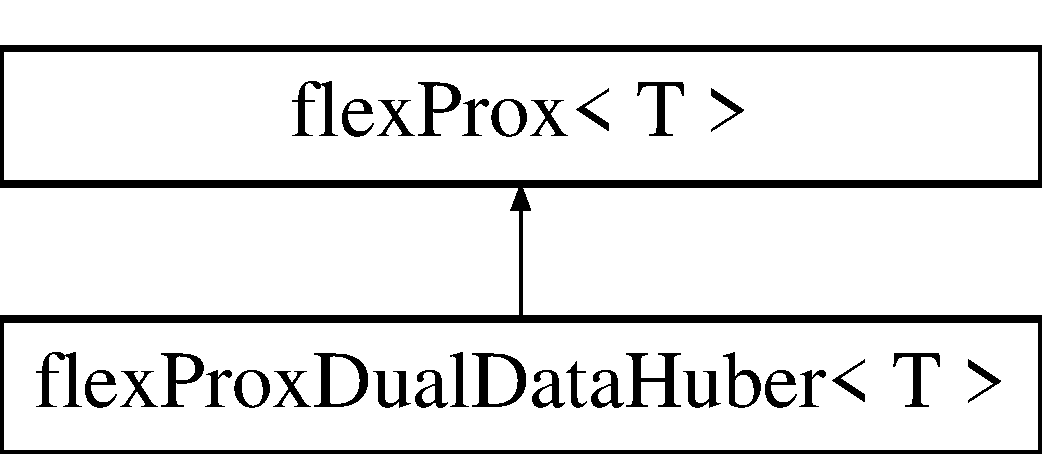
\includegraphics[height=2.000000cm]{classflex_prox_dual_data_huber}
\end{center}
\end{figure}
\subsection*{Classes}
\begin{DoxyCompactItemize}
\item 
struct {\bfseries flex\+Prox\+Dual\+Data\+L1\+Functor}
\end{DoxyCompactItemize}
\subsection*{Public Member Functions}
\begin{DoxyCompactItemize}
\item 
\mbox{\Hypertarget{classflex_prox_dual_data_huber_a22b6028c5e11ac8560c528a5ce82a3af}\label{classflex_prox_dual_data_huber_a22b6028c5e11ac8560c528a5ce82a3af}} 
{\bfseries flex\+Prox\+Dual\+Data\+Huber} (T a\+Huber\+Epsilon)
\item 
void \hyperlink{classflex_prox_dual_data_huber_ac085f34619c3d747b09a2b369a11dcd5}{apply\+Prox} (T alpha, \hyperlink{classflex_box_data}{flex\+Box\+Data}$<$ T $>$ $\ast$data, const std\+::vector$<$ int $>$ \&dual\+Numbers, const std\+::vector$<$ int $>$ \&primal\+Numbers)
\begin{DoxyCompactList}\small\item\em applies prox for non-\/data terms \end{DoxyCompactList}\item 
void \hyperlink{classflex_prox_dual_data_huber_ab1c0bbd454ee7fe65592ff8beda4aaa5}{apply\+Prox} (T alpha, \hyperlink{classflex_box_data}{flex\+Box\+Data}$<$ T $>$ $\ast$data, const std\+::vector$<$ int $>$ \&dual\+Numbers, const std\+::vector$<$ int $>$ \&primal\+Numbers, std\+::vector$<$ Tdata $>$ \&f\+List)
\begin{DoxyCompactList}\small\item\em applies prox for data terms \end{DoxyCompactList}\end{DoxyCompactItemize}
\subsection*{Additional Inherited Members}


\subsection{Detailed Description}
\subsubsection*{template$<$typename T$>$\newline
class flex\+Prox\+Dual\+Data\+Huber$<$ T $>$}

represents prox for a Huber data term 

$ \alpha\|\cdot-f\|_\epsilon $ 

\subsection{Member Function Documentation}
\mbox{\Hypertarget{classflex_prox_dual_data_huber_ac085f34619c3d747b09a2b369a11dcd5}\label{classflex_prox_dual_data_huber_ac085f34619c3d747b09a2b369a11dcd5}} 
\index{flex\+Prox\+Dual\+Data\+Huber@{flex\+Prox\+Dual\+Data\+Huber}!apply\+Prox@{apply\+Prox}}
\index{apply\+Prox@{apply\+Prox}!flex\+Prox\+Dual\+Data\+Huber@{flex\+Prox\+Dual\+Data\+Huber}}
\subsubsection{\texorpdfstring{apply\+Prox()}{applyProx()}\hspace{0.1cm}{\footnotesize\ttfamily [1/2]}}
{\footnotesize\ttfamily template$<$typename T $>$ \\
void \hyperlink{classflex_prox_dual_data_huber}{flex\+Prox\+Dual\+Data\+Huber}$<$ T $>$\+::apply\+Prox (\begin{DoxyParamCaption}\item[{T}]{alpha,  }\item[{\hyperlink{classflex_box_data}{flex\+Box\+Data}$<$ T $>$ $\ast$}]{data,  }\item[{const std\+::vector$<$ int $>$ \&}]{dual\+Numbers,  }\item[{const std\+::vector$<$ int $>$ \&}]{primal\+Numbers }\end{DoxyParamCaption})\hspace{0.3cm}{\ttfamily [inline]}, {\ttfamily [virtual]}}



applies prox for non-\/data terms 

the function body should be empty if implemented prox is a data prox 
\begin{DoxyParams}{Parameters}
{\em alpha} & weight of term \\
\hline
{\em data} & data object \\
\hline
{\em dual\+Numbers} & vector of internal identifactions of dual numbers corresponding to the term \\
\hline
\end{DoxyParams}
\begin{DoxySeeAlso}{See also}
\hyperlink{classflex_box}{flex\+Box} 
\end{DoxySeeAlso}

\begin{DoxyParams}{Parameters}
{\em primal\+Numbers} & vector of internal identifactions of primal numbers corresponding to the term \\
\hline
\end{DoxyParams}
\begin{DoxySeeAlso}{See also}
\hyperlink{classflex_box}{flex\+Box} 
\end{DoxySeeAlso}


Implements \hyperlink{classflex_prox_a6d3119bd368c4216ad264a1f6dc1d01f}{flex\+Prox$<$ T $>$}.

\mbox{\Hypertarget{classflex_prox_dual_data_huber_ab1c0bbd454ee7fe65592ff8beda4aaa5}\label{classflex_prox_dual_data_huber_ab1c0bbd454ee7fe65592ff8beda4aaa5}} 
\index{flex\+Prox\+Dual\+Data\+Huber@{flex\+Prox\+Dual\+Data\+Huber}!apply\+Prox@{apply\+Prox}}
\index{apply\+Prox@{apply\+Prox}!flex\+Prox\+Dual\+Data\+Huber@{flex\+Prox\+Dual\+Data\+Huber}}
\subsubsection{\texorpdfstring{apply\+Prox()}{applyProx()}\hspace{0.1cm}{\footnotesize\ttfamily [2/2]}}
{\footnotesize\ttfamily template$<$typename T $>$ \\
void \hyperlink{classflex_prox_dual_data_huber}{flex\+Prox\+Dual\+Data\+Huber}$<$ T $>$\+::apply\+Prox (\begin{DoxyParamCaption}\item[{T}]{alpha,  }\item[{\hyperlink{classflex_box_data}{flex\+Box\+Data}$<$ T $>$ $\ast$}]{data,  }\item[{const std\+::vector$<$ int $>$ \&}]{dual\+Numbers,  }\item[{const std\+::vector$<$ int $>$ \&}]{primal\+Numbers,  }\item[{std\+::vector$<$ Tdata $>$ \&}]{f\+List }\end{DoxyParamCaption})\hspace{0.3cm}{\ttfamily [inline]}, {\ttfamily [virtual]}}



applies prox for data terms 

the function body should be empty if implemented prox is a non-\/data prox 
\begin{DoxyParams}{Parameters}
{\em alpha} & weight of term \\
\hline
{\em data} & data object \\
\hline
{\em dual\+Numbers} & vector of internal identifactions of dual numbers corresponding to the term \\
\hline
\end{DoxyParams}
\begin{DoxySeeAlso}{See also}
\hyperlink{classflex_box}{flex\+Box} 
\end{DoxySeeAlso}

\begin{DoxyParams}{Parameters}
{\em primal\+Numbers} & vector of internal identifactions of primal numbers corresponding to the term \\
\hline
\end{DoxyParams}
\begin{DoxySeeAlso}{See also}
\hyperlink{classflex_box}{flex\+Box} 
\end{DoxySeeAlso}

\begin{DoxyParams}{Parameters}
{\em f\+List} & data part of term \\
\hline
\end{DoxyParams}


Implements \hyperlink{classflex_prox_aec433ffbf1a7586f26a2116c6b94bdd6}{flex\+Prox$<$ T $>$}.



The documentation for this class was generated from the following file\+:\begin{DoxyCompactItemize}
\item 
flex\+Prox\+Dual\+Data\+Huber.\+h\end{DoxyCompactItemize}

\hypertarget{classflex_prox_dual_data_k_l}{}\section{flex\+Prox\+Dual\+Data\+KL$<$ T $>$ Class Template Reference}
\label{classflex_prox_dual_data_k_l}\index{flex\+Prox\+Dual\+Data\+K\+L$<$ T $>$@{flex\+Prox\+Dual\+Data\+K\+L$<$ T $>$}}


represents prox for a Kullback-\/\+Leibler divergence data term  




{\ttfamily \#include $<$flex\+Prox\+Dual\+Data\+K\+L.\+h$>$}

Inheritance diagram for flex\+Prox\+Dual\+Data\+KL$<$ T $>$\+:\begin{figure}[H]
\begin{center}
\leavevmode
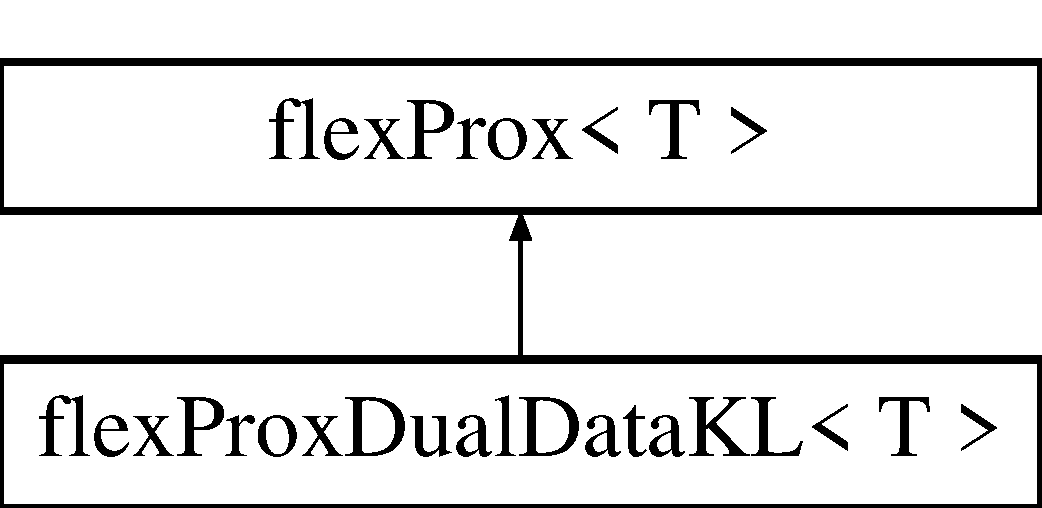
\includegraphics[height=2.000000cm]{classflex_prox_dual_data_k_l}
\end{center}
\end{figure}
\subsection*{Classes}
\begin{DoxyCompactItemize}
\item 
struct {\bfseries flex\+Prox\+Dual\+Data\+K\+L\+Functor}
\end{DoxyCompactItemize}
\subsection*{Public Member Functions}
\begin{DoxyCompactItemize}
\item 
void \hyperlink{classflex_prox_dual_data_k_l_ad6314cbdf307759e3176e26b3efba7c6}{apply\+Prox} (T alpha, \hyperlink{classflex_box_data}{flex\+Box\+Data}$<$ T $>$ $\ast$data, const std\+::vector$<$ int $>$ \&dual\+Numbers, const std\+::vector$<$ int $>$ \&primal\+Numbers)
\begin{DoxyCompactList}\small\item\em applies prox for non-\/data terms \end{DoxyCompactList}\item 
void \hyperlink{classflex_prox_dual_data_k_l_aa02947fd71697cdb7d6d7e0d617fdfc3}{apply\+Prox} (T alpha, \hyperlink{classflex_box_data}{flex\+Box\+Data}$<$ T $>$ $\ast$data, const std\+::vector$<$ int $>$ \&dual\+Numbers, const std\+::vector$<$ int $>$ \&primal\+Numbers, std\+::vector$<$ Tdata $>$ \&f\+List)
\begin{DoxyCompactList}\small\item\em applies prox for data terms \end{DoxyCompactList}\end{DoxyCompactItemize}
\subsection*{Additional Inherited Members}


\subsection{Detailed Description}
\subsubsection*{template$<$typename T$>$\newline
class flex\+Prox\+Dual\+Data\+K\+L$<$ T $>$}

represents prox for a Kullback-\/\+Leibler divergence data term 

$ \alpha(\cdot-f+f\log\frac{f}{\cdot} + \delta_{\{\bar{u} : \bar{u}> 0 \}}(\cdot)) $ 

\subsection{Member Function Documentation}
\mbox{\Hypertarget{classflex_prox_dual_data_k_l_ad6314cbdf307759e3176e26b3efba7c6}\label{classflex_prox_dual_data_k_l_ad6314cbdf307759e3176e26b3efba7c6}} 
\index{flex\+Prox\+Dual\+Data\+KL@{flex\+Prox\+Dual\+Data\+KL}!apply\+Prox@{apply\+Prox}}
\index{apply\+Prox@{apply\+Prox}!flex\+Prox\+Dual\+Data\+KL@{flex\+Prox\+Dual\+Data\+KL}}
\subsubsection{\texorpdfstring{apply\+Prox()}{applyProx()}\hspace{0.1cm}{\footnotesize\ttfamily [1/2]}}
{\footnotesize\ttfamily template$<$typename T $>$ \\
void \hyperlink{classflex_prox_dual_data_k_l}{flex\+Prox\+Dual\+Data\+KL}$<$ T $>$\+::apply\+Prox (\begin{DoxyParamCaption}\item[{T}]{alpha,  }\item[{\hyperlink{classflex_box_data}{flex\+Box\+Data}$<$ T $>$ $\ast$}]{data,  }\item[{const std\+::vector$<$ int $>$ \&}]{dual\+Numbers,  }\item[{const std\+::vector$<$ int $>$ \&}]{primal\+Numbers }\end{DoxyParamCaption})\hspace{0.3cm}{\ttfamily [inline]}, {\ttfamily [virtual]}}



applies prox for non-\/data terms 

the function body should be empty if implemented prox is a data prox 
\begin{DoxyParams}{Parameters}
{\em alpha} & weight of term \\
\hline
{\em data} & data object \\
\hline
{\em dual\+Numbers} & vector of internal identifactions of dual numbers corresponding to the term \\
\hline
\end{DoxyParams}
\begin{DoxySeeAlso}{See also}
\hyperlink{classflex_box}{flex\+Box} 
\end{DoxySeeAlso}

\begin{DoxyParams}{Parameters}
{\em primal\+Numbers} & vector of internal identifactions of primal numbers corresponding to the term \\
\hline
\end{DoxyParams}
\begin{DoxySeeAlso}{See also}
\hyperlink{classflex_box}{flex\+Box} 
\end{DoxySeeAlso}


Implements \hyperlink{classflex_prox_a6d3119bd368c4216ad264a1f6dc1d01f}{flex\+Prox$<$ T $>$}.

\mbox{\Hypertarget{classflex_prox_dual_data_k_l_aa02947fd71697cdb7d6d7e0d617fdfc3}\label{classflex_prox_dual_data_k_l_aa02947fd71697cdb7d6d7e0d617fdfc3}} 
\index{flex\+Prox\+Dual\+Data\+KL@{flex\+Prox\+Dual\+Data\+KL}!apply\+Prox@{apply\+Prox}}
\index{apply\+Prox@{apply\+Prox}!flex\+Prox\+Dual\+Data\+KL@{flex\+Prox\+Dual\+Data\+KL}}
\subsubsection{\texorpdfstring{apply\+Prox()}{applyProx()}\hspace{0.1cm}{\footnotesize\ttfamily [2/2]}}
{\footnotesize\ttfamily template$<$typename T $>$ \\
void \hyperlink{classflex_prox_dual_data_k_l}{flex\+Prox\+Dual\+Data\+KL}$<$ T $>$\+::apply\+Prox (\begin{DoxyParamCaption}\item[{T}]{alpha,  }\item[{\hyperlink{classflex_box_data}{flex\+Box\+Data}$<$ T $>$ $\ast$}]{data,  }\item[{const std\+::vector$<$ int $>$ \&}]{dual\+Numbers,  }\item[{const std\+::vector$<$ int $>$ \&}]{primal\+Numbers,  }\item[{std\+::vector$<$ Tdata $>$ \&}]{f\+List }\end{DoxyParamCaption})\hspace{0.3cm}{\ttfamily [inline]}, {\ttfamily [virtual]}}



applies prox for data terms 

the function body should be empty if implemented prox is a non-\/data prox 
\begin{DoxyParams}{Parameters}
{\em alpha} & weight of term \\
\hline
{\em data} & data object \\
\hline
{\em dual\+Numbers} & vector of internal identifactions of dual numbers corresponding to the term \\
\hline
\end{DoxyParams}
\begin{DoxySeeAlso}{See also}
\hyperlink{classflex_box}{flex\+Box} 
\end{DoxySeeAlso}

\begin{DoxyParams}{Parameters}
{\em primal\+Numbers} & vector of internal identifactions of primal numbers corresponding to the term \\
\hline
\end{DoxyParams}
\begin{DoxySeeAlso}{See also}
\hyperlink{classflex_box}{flex\+Box} 
\end{DoxySeeAlso}

\begin{DoxyParams}{Parameters}
{\em f\+List} & data part of term \\
\hline
\end{DoxyParams}


Implements \hyperlink{classflex_prox_aec433ffbf1a7586f26a2116c6b94bdd6}{flex\+Prox$<$ T $>$}.



The documentation for this class was generated from the following file\+:\begin{DoxyCompactItemize}
\item 
flex\+Prox\+Dual\+Data\+K\+L.\+h\end{DoxyCompactItemize}

\hypertarget{classflex_prox_dual_data_l1}{}\section{flex\+Prox\+Dual\+Data\+L1$<$ T $>$ Class Template Reference}
\label{classflex_prox_dual_data_l1}\index{flex\+Prox\+Dual\+Data\+L1$<$ T $>$@{flex\+Prox\+Dual\+Data\+L1$<$ T $>$}}


represents prox for a L1 data term  




{\ttfamily \#include $<$flex\+Prox\+Dual\+Data\+L1.\+h$>$}

Inheritance diagram for flex\+Prox\+Dual\+Data\+L1$<$ T $>$\+:\begin{figure}[H]
\begin{center}
\leavevmode
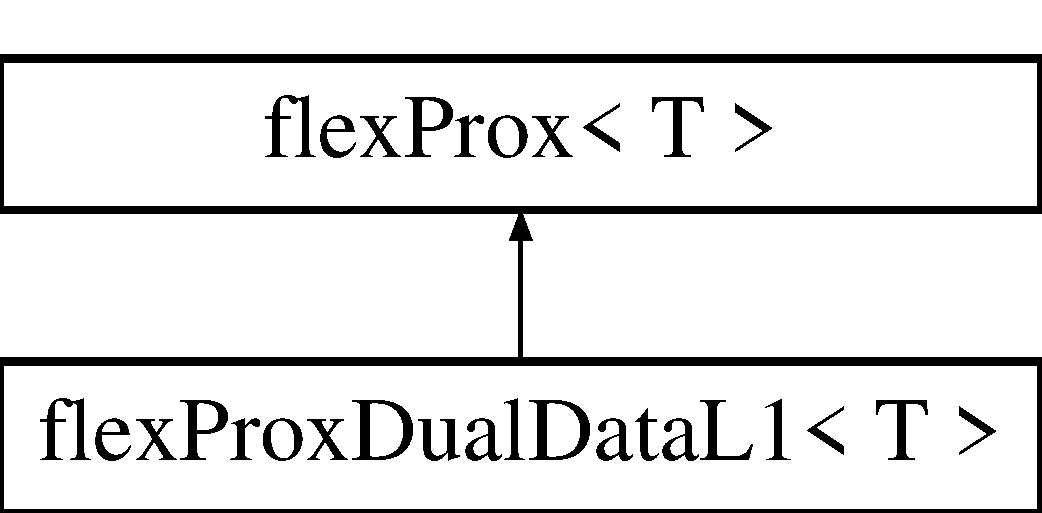
\includegraphics[height=2.000000cm]{classflex_prox_dual_data_l1}
\end{center}
\end{figure}
\subsection*{Classes}
\begin{DoxyCompactItemize}
\item 
struct {\bfseries flex\+Prox\+Dual\+Data\+L1\+Functor}
\end{DoxyCompactItemize}
\subsection*{Public Member Functions}
\begin{DoxyCompactItemize}
\item 
void \hyperlink{classflex_prox_dual_data_l1_a8ebb08fae14a70bc6ed15b6d75b67705}{apply\+Prox} (T alpha, \hyperlink{classflex_box_data}{flex\+Box\+Data}$<$ T $>$ $\ast$data, const std\+::vector$<$ int $>$ \&dual\+Numbers, const std\+::vector$<$ int $>$ \&primal\+Numbers)
\begin{DoxyCompactList}\small\item\em applies prox for non-\/data terms \end{DoxyCompactList}\item 
void \hyperlink{classflex_prox_dual_data_l1_a3487ee84a12852486a1639d3b9dea735}{apply\+Prox} (T alpha, \hyperlink{classflex_box_data}{flex\+Box\+Data}$<$ T $>$ $\ast$data, const std\+::vector$<$ int $>$ \&dual\+Numbers, const std\+::vector$<$ int $>$ \&primal\+Numbers, std\+::vector$<$ Tdata $>$ \&f\+List)
\begin{DoxyCompactList}\small\item\em applies prox for data terms \end{DoxyCompactList}\end{DoxyCompactItemize}
\subsection*{Additional Inherited Members}


\subsection{Detailed Description}
\subsubsection*{template$<$typename T$>$\newline
class flex\+Prox\+Dual\+Data\+L1$<$ T $>$}

represents prox for a L1 data term 

$ \alpha\|\cdot-f\|_1 $ 

\subsection{Member Function Documentation}
\mbox{\Hypertarget{classflex_prox_dual_data_l1_a8ebb08fae14a70bc6ed15b6d75b67705}\label{classflex_prox_dual_data_l1_a8ebb08fae14a70bc6ed15b6d75b67705}} 
\index{flex\+Prox\+Dual\+Data\+L1@{flex\+Prox\+Dual\+Data\+L1}!apply\+Prox@{apply\+Prox}}
\index{apply\+Prox@{apply\+Prox}!flex\+Prox\+Dual\+Data\+L1@{flex\+Prox\+Dual\+Data\+L1}}
\subsubsection{\texorpdfstring{apply\+Prox()}{applyProx()}\hspace{0.1cm}{\footnotesize\ttfamily [1/2]}}
{\footnotesize\ttfamily template$<$typename T $>$ \\
void \hyperlink{classflex_prox_dual_data_l1}{flex\+Prox\+Dual\+Data\+L1}$<$ T $>$\+::apply\+Prox (\begin{DoxyParamCaption}\item[{T}]{alpha,  }\item[{\hyperlink{classflex_box_data}{flex\+Box\+Data}$<$ T $>$ $\ast$}]{data,  }\item[{const std\+::vector$<$ int $>$ \&}]{dual\+Numbers,  }\item[{const std\+::vector$<$ int $>$ \&}]{primal\+Numbers }\end{DoxyParamCaption})\hspace{0.3cm}{\ttfamily [inline]}, {\ttfamily [virtual]}}



applies prox for non-\/data terms 

the function body should be empty if implemented prox is a data prox 
\begin{DoxyParams}{Parameters}
{\em alpha} & weight of term \\
\hline
{\em data} & data object \\
\hline
{\em dual\+Numbers} & vector of internal identifactions of dual numbers corresponding to the term \\
\hline
\end{DoxyParams}
\begin{DoxySeeAlso}{See also}
\hyperlink{classflex_box}{flex\+Box} 
\end{DoxySeeAlso}

\begin{DoxyParams}{Parameters}
{\em primal\+Numbers} & vector of internal identifactions of primal numbers corresponding to the term \\
\hline
\end{DoxyParams}
\begin{DoxySeeAlso}{See also}
\hyperlink{classflex_box}{flex\+Box} 
\end{DoxySeeAlso}


Implements \hyperlink{classflex_prox_a6d3119bd368c4216ad264a1f6dc1d01f}{flex\+Prox$<$ T $>$}.

\mbox{\Hypertarget{classflex_prox_dual_data_l1_a3487ee84a12852486a1639d3b9dea735}\label{classflex_prox_dual_data_l1_a3487ee84a12852486a1639d3b9dea735}} 
\index{flex\+Prox\+Dual\+Data\+L1@{flex\+Prox\+Dual\+Data\+L1}!apply\+Prox@{apply\+Prox}}
\index{apply\+Prox@{apply\+Prox}!flex\+Prox\+Dual\+Data\+L1@{flex\+Prox\+Dual\+Data\+L1}}
\subsubsection{\texorpdfstring{apply\+Prox()}{applyProx()}\hspace{0.1cm}{\footnotesize\ttfamily [2/2]}}
{\footnotesize\ttfamily template$<$typename T $>$ \\
void \hyperlink{classflex_prox_dual_data_l1}{flex\+Prox\+Dual\+Data\+L1}$<$ T $>$\+::apply\+Prox (\begin{DoxyParamCaption}\item[{T}]{alpha,  }\item[{\hyperlink{classflex_box_data}{flex\+Box\+Data}$<$ T $>$ $\ast$}]{data,  }\item[{const std\+::vector$<$ int $>$ \&}]{dual\+Numbers,  }\item[{const std\+::vector$<$ int $>$ \&}]{primal\+Numbers,  }\item[{std\+::vector$<$ Tdata $>$ \&}]{f\+List }\end{DoxyParamCaption})\hspace{0.3cm}{\ttfamily [inline]}, {\ttfamily [virtual]}}



applies prox for data terms 

the function body should be empty if implemented prox is a non-\/data prox 
\begin{DoxyParams}{Parameters}
{\em alpha} & weight of term \\
\hline
{\em data} & data object \\
\hline
{\em dual\+Numbers} & vector of internal identifactions of dual numbers corresponding to the term \\
\hline
\end{DoxyParams}
\begin{DoxySeeAlso}{See also}
\hyperlink{classflex_box}{flex\+Box} 
\end{DoxySeeAlso}

\begin{DoxyParams}{Parameters}
{\em primal\+Numbers} & vector of internal identifactions of primal numbers corresponding to the term \\
\hline
\end{DoxyParams}
\begin{DoxySeeAlso}{See also}
\hyperlink{classflex_box}{flex\+Box} 
\end{DoxySeeAlso}

\begin{DoxyParams}{Parameters}
{\em f\+List} & data part of term \\
\hline
\end{DoxyParams}


Implements \hyperlink{classflex_prox_aec433ffbf1a7586f26a2116c6b94bdd6}{flex\+Prox$<$ T $>$}.



The documentation for this class was generated from the following file\+:\begin{DoxyCompactItemize}
\item 
flex\+Prox\+Dual\+Data\+L1.\+h\end{DoxyCompactItemize}

\hypertarget{classflex_prox_dual_data_l2}{}\section{flex\+Prox\+Dual\+Data\+L2$<$ T $>$ Class Template Reference}
\label{classflex_prox_dual_data_l2}\index{flex\+Prox\+Dual\+Data\+L2$<$ T $>$@{flex\+Prox\+Dual\+Data\+L2$<$ T $>$}}


represents prox for a L2 data term  




{\ttfamily \#include $<$flex\+Prox\+Dual\+Data\+L2.\+h$>$}

Inheritance diagram for flex\+Prox\+Dual\+Data\+L2$<$ T $>$\+:\begin{figure}[H]
\begin{center}
\leavevmode
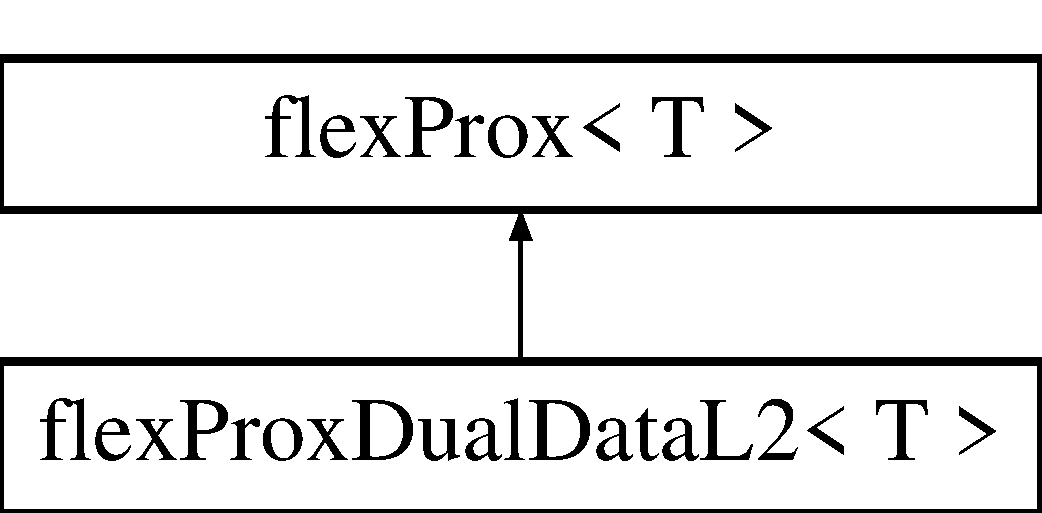
\includegraphics[height=2.000000cm]{classflex_prox_dual_data_l2}
\end{center}
\end{figure}
\subsection*{Classes}
\begin{DoxyCompactItemize}
\item 
struct {\bfseries flex\+Prox\+Dual\+Data\+L2\+Functor}
\end{DoxyCompactItemize}
\subsection*{Public Member Functions}
\begin{DoxyCompactItemize}
\item 
void \hyperlink{classflex_prox_dual_data_l2_ae3ee176dc6c05e8fba0df96c73b10464}{apply\+Prox} (T alpha, \hyperlink{classflex_box_data}{flex\+Box\+Data}$<$ T $>$ $\ast$data, const std\+::vector$<$ int $>$ \&dual\+Numbers, const std\+::vector$<$ int $>$ \&primal\+Numbers)
\begin{DoxyCompactList}\small\item\em applies prox for non-\/data terms \end{DoxyCompactList}\item 
void \hyperlink{classflex_prox_dual_data_l2_a0d7a54201b01863a9a76f6fc2d52cf22}{apply\+Prox} (T alpha, \hyperlink{classflex_box_data}{flex\+Box\+Data}$<$ T $>$ $\ast$data, const std\+::vector$<$ int $>$ \&dual\+Numbers, const std\+::vector$<$ int $>$ \&primal\+Numbers, std\+::vector$<$ Tdata $>$ \&f\+List)
\begin{DoxyCompactList}\small\item\em applies prox for data terms \end{DoxyCompactList}\end{DoxyCompactItemize}
\subsection*{Additional Inherited Members}


\subsection{Detailed Description}
\subsubsection*{template$<$typename T$>$\newline
class flex\+Prox\+Dual\+Data\+L2$<$ T $>$}

represents prox for a L2 data term 

$ \frac{\alpha}{2}\|\cdot-f\|_2^2 $ 

\subsection{Member Function Documentation}
\mbox{\Hypertarget{classflex_prox_dual_data_l2_ae3ee176dc6c05e8fba0df96c73b10464}\label{classflex_prox_dual_data_l2_ae3ee176dc6c05e8fba0df96c73b10464}} 
\index{flex\+Prox\+Dual\+Data\+L2@{flex\+Prox\+Dual\+Data\+L2}!apply\+Prox@{apply\+Prox}}
\index{apply\+Prox@{apply\+Prox}!flex\+Prox\+Dual\+Data\+L2@{flex\+Prox\+Dual\+Data\+L2}}
\subsubsection{\texorpdfstring{apply\+Prox()}{applyProx()}\hspace{0.1cm}{\footnotesize\ttfamily [1/2]}}
{\footnotesize\ttfamily template$<$typename T $>$ \\
void \hyperlink{classflex_prox_dual_data_l2}{flex\+Prox\+Dual\+Data\+L2}$<$ T $>$\+::apply\+Prox (\begin{DoxyParamCaption}\item[{T}]{alpha,  }\item[{\hyperlink{classflex_box_data}{flex\+Box\+Data}$<$ T $>$ $\ast$}]{data,  }\item[{const std\+::vector$<$ int $>$ \&}]{dual\+Numbers,  }\item[{const std\+::vector$<$ int $>$ \&}]{primal\+Numbers }\end{DoxyParamCaption})\hspace{0.3cm}{\ttfamily [inline]}, {\ttfamily [virtual]}}



applies prox for non-\/data terms 

the function body should be empty if implemented prox is a data prox 
\begin{DoxyParams}{Parameters}
{\em alpha} & weight of term \\
\hline
{\em data} & data object \\
\hline
{\em dual\+Numbers} & vector of internal identifactions of dual numbers corresponding to the term \\
\hline
\end{DoxyParams}
\begin{DoxySeeAlso}{See also}
\hyperlink{classflex_box}{flex\+Box} 
\end{DoxySeeAlso}

\begin{DoxyParams}{Parameters}
{\em primal\+Numbers} & vector of internal identifactions of primal numbers corresponding to the term \\
\hline
\end{DoxyParams}
\begin{DoxySeeAlso}{See also}
\hyperlink{classflex_box}{flex\+Box} 
\end{DoxySeeAlso}


Implements \hyperlink{classflex_prox_a6d3119bd368c4216ad264a1f6dc1d01f}{flex\+Prox$<$ T $>$}.

\mbox{\Hypertarget{classflex_prox_dual_data_l2_a0d7a54201b01863a9a76f6fc2d52cf22}\label{classflex_prox_dual_data_l2_a0d7a54201b01863a9a76f6fc2d52cf22}} 
\index{flex\+Prox\+Dual\+Data\+L2@{flex\+Prox\+Dual\+Data\+L2}!apply\+Prox@{apply\+Prox}}
\index{apply\+Prox@{apply\+Prox}!flex\+Prox\+Dual\+Data\+L2@{flex\+Prox\+Dual\+Data\+L2}}
\subsubsection{\texorpdfstring{apply\+Prox()}{applyProx()}\hspace{0.1cm}{\footnotesize\ttfamily [2/2]}}
{\footnotesize\ttfamily template$<$typename T $>$ \\
void \hyperlink{classflex_prox_dual_data_l2}{flex\+Prox\+Dual\+Data\+L2}$<$ T $>$\+::apply\+Prox (\begin{DoxyParamCaption}\item[{T}]{alpha,  }\item[{\hyperlink{classflex_box_data}{flex\+Box\+Data}$<$ T $>$ $\ast$}]{data,  }\item[{const std\+::vector$<$ int $>$ \&}]{dual\+Numbers,  }\item[{const std\+::vector$<$ int $>$ \&}]{primal\+Numbers,  }\item[{std\+::vector$<$ Tdata $>$ \&}]{f\+List }\end{DoxyParamCaption})\hspace{0.3cm}{\ttfamily [inline]}, {\ttfamily [virtual]}}



applies prox for data terms 

the function body should be empty if implemented prox is a non-\/data prox 
\begin{DoxyParams}{Parameters}
{\em alpha} & weight of term \\
\hline
{\em data} & data object \\
\hline
{\em dual\+Numbers} & vector of internal identifactions of dual numbers corresponding to the term \\
\hline
\end{DoxyParams}
\begin{DoxySeeAlso}{See also}
\hyperlink{classflex_box}{flex\+Box} 
\end{DoxySeeAlso}

\begin{DoxyParams}{Parameters}
{\em primal\+Numbers} & vector of internal identifactions of primal numbers corresponding to the term \\
\hline
\end{DoxyParams}
\begin{DoxySeeAlso}{See also}
\hyperlink{classflex_box}{flex\+Box} 
\end{DoxySeeAlso}

\begin{DoxyParams}{Parameters}
{\em f\+List} & data part of term \\
\hline
\end{DoxyParams}


Implements \hyperlink{classflex_prox_aec433ffbf1a7586f26a2116c6b94bdd6}{flex\+Prox$<$ T $>$}.



The documentation for this class was generated from the following file\+:\begin{DoxyCompactItemize}
\item 
flex\+Prox\+Dual\+Data\+L2.\+h\end{DoxyCompactItemize}

\hypertarget{classflex_prox_dual_frobenius}{}\section{flex\+Prox\+Dual\+Frobenius$<$ T $>$ Class Template Reference}
\label{classflex_prox_dual_frobenius}\index{flex\+Prox\+Dual\+Frobenius$<$ T $>$@{flex\+Prox\+Dual\+Frobenius$<$ T $>$}}


represents prox for a Frobenius term  




{\ttfamily \#include $<$flex\+Prox\+Dual\+Frobenius.\+h$>$}

Inheritance diagram for flex\+Prox\+Dual\+Frobenius$<$ T $>$\+:\begin{figure}[H]
\begin{center}
\leavevmode
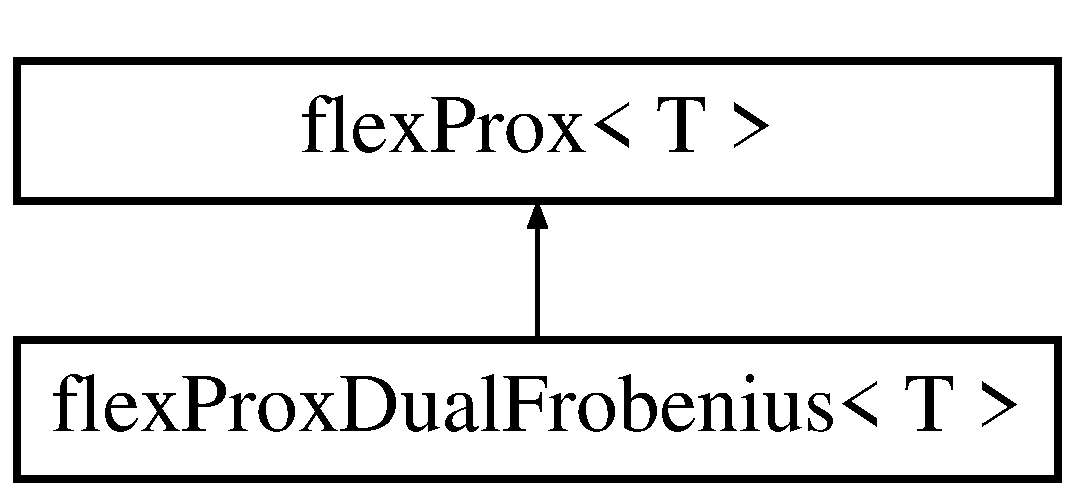
\includegraphics[height=2.000000cm]{classflex_prox_dual_frobenius}
\end{center}
\end{figure}
\subsection*{Classes}
\begin{DoxyCompactItemize}
\item 
struct {\bfseries flex\+Frobenius\+Square\+Functor}
\item 
struct {\bfseries flex\+Prox\+Dual\+Frobenius\+Functor}
\end{DoxyCompactItemize}
\subsection*{Public Member Functions}
\begin{DoxyCompactItemize}
\item 
void \hyperlink{classflex_prox_dual_frobenius_a08de45a25d007ea87379641d027fd228}{apply\+Prox} (T alpha, \hyperlink{classflex_box_data}{flex\+Box\+Data}$<$ T $>$ $\ast$data, const std\+::vector$<$ int $>$ \&dual\+Numbers, const std\+::vector$<$ int $>$ \&primal\+Numbers)
\begin{DoxyCompactList}\small\item\em applies prox for non-\/data terms \end{DoxyCompactList}\item 
void \hyperlink{classflex_prox_dual_frobenius_a24695ced8a80693606e1654b04bd068f}{apply\+Prox} (T alpha, \hyperlink{classflex_box_data}{flex\+Box\+Data}$<$ T $>$ $\ast$data, const std\+::vector$<$ int $>$ \&dual\+Numbers, const std\+::vector$<$ int $>$ \&primal\+Numbers, std\+::vector$<$ Tdata $>$ \&f\+List)
\begin{DoxyCompactList}\small\item\em applies prox for data terms \end{DoxyCompactList}\end{DoxyCompactItemize}
\subsection*{Additional Inherited Members}


\subsection{Detailed Description}
\subsubsection*{template$<$typename T$>$\newline
class flex\+Prox\+Dual\+Frobenius$<$ T $>$}

represents prox for a Frobenius term 

$ \alpha\|\cdot\|_{F} $ 

\subsection{Member Function Documentation}
\mbox{\Hypertarget{classflex_prox_dual_frobenius_a08de45a25d007ea87379641d027fd228}\label{classflex_prox_dual_frobenius_a08de45a25d007ea87379641d027fd228}} 
\index{flex\+Prox\+Dual\+Frobenius@{flex\+Prox\+Dual\+Frobenius}!apply\+Prox@{apply\+Prox}}
\index{apply\+Prox@{apply\+Prox}!flex\+Prox\+Dual\+Frobenius@{flex\+Prox\+Dual\+Frobenius}}
\subsubsection{\texorpdfstring{apply\+Prox()}{applyProx()}\hspace{0.1cm}{\footnotesize\ttfamily [1/2]}}
{\footnotesize\ttfamily template$<$typename T $>$ \\
void \hyperlink{classflex_prox_dual_frobenius}{flex\+Prox\+Dual\+Frobenius}$<$ T $>$\+::apply\+Prox (\begin{DoxyParamCaption}\item[{T}]{alpha,  }\item[{\hyperlink{classflex_box_data}{flex\+Box\+Data}$<$ T $>$ $\ast$}]{data,  }\item[{const std\+::vector$<$ int $>$ \&}]{dual\+Numbers,  }\item[{const std\+::vector$<$ int $>$ \&}]{primal\+Numbers }\end{DoxyParamCaption})\hspace{0.3cm}{\ttfamily [inline]}, {\ttfamily [virtual]}}



applies prox for non-\/data terms 

the function body should be empty if implemented prox is a data prox 
\begin{DoxyParams}{Parameters}
{\em alpha} & weight of term \\
\hline
{\em data} & data object \\
\hline
{\em dual\+Numbers} & vector of internal identifactions of dual numbers corresponding to the term \\
\hline
\end{DoxyParams}
\begin{DoxySeeAlso}{See also}
\hyperlink{classflex_box}{flex\+Box} 
\end{DoxySeeAlso}

\begin{DoxyParams}{Parameters}
{\em primal\+Numbers} & vector of internal identifactions of primal numbers corresponding to the term \\
\hline
\end{DoxyParams}
\begin{DoxySeeAlso}{See also}
\hyperlink{classflex_box}{flex\+Box} 
\end{DoxySeeAlso}


Implements \hyperlink{classflex_prox_a6d3119bd368c4216ad264a1f6dc1d01f}{flex\+Prox$<$ T $>$}.

\mbox{\Hypertarget{classflex_prox_dual_frobenius_a24695ced8a80693606e1654b04bd068f}\label{classflex_prox_dual_frobenius_a24695ced8a80693606e1654b04bd068f}} 
\index{flex\+Prox\+Dual\+Frobenius@{flex\+Prox\+Dual\+Frobenius}!apply\+Prox@{apply\+Prox}}
\index{apply\+Prox@{apply\+Prox}!flex\+Prox\+Dual\+Frobenius@{flex\+Prox\+Dual\+Frobenius}}
\subsubsection{\texorpdfstring{apply\+Prox()}{applyProx()}\hspace{0.1cm}{\footnotesize\ttfamily [2/2]}}
{\footnotesize\ttfamily template$<$typename T $>$ \\
void \hyperlink{classflex_prox_dual_frobenius}{flex\+Prox\+Dual\+Frobenius}$<$ T $>$\+::apply\+Prox (\begin{DoxyParamCaption}\item[{T}]{alpha,  }\item[{\hyperlink{classflex_box_data}{flex\+Box\+Data}$<$ T $>$ $\ast$}]{data,  }\item[{const std\+::vector$<$ int $>$ \&}]{dual\+Numbers,  }\item[{const std\+::vector$<$ int $>$ \&}]{primal\+Numbers,  }\item[{std\+::vector$<$ Tdata $>$ \&}]{f\+List }\end{DoxyParamCaption})\hspace{0.3cm}{\ttfamily [inline]}, {\ttfamily [virtual]}}



applies prox for data terms 

the function body should be empty if implemented prox is a non-\/data prox 
\begin{DoxyParams}{Parameters}
{\em alpha} & weight of term \\
\hline
{\em data} & data object \\
\hline
{\em dual\+Numbers} & vector of internal identifactions of dual numbers corresponding to the term \\
\hline
\end{DoxyParams}
\begin{DoxySeeAlso}{See also}
\hyperlink{classflex_box}{flex\+Box} 
\end{DoxySeeAlso}

\begin{DoxyParams}{Parameters}
{\em primal\+Numbers} & vector of internal identifactions of primal numbers corresponding to the term \\
\hline
\end{DoxyParams}
\begin{DoxySeeAlso}{See also}
\hyperlink{classflex_box}{flex\+Box} 
\end{DoxySeeAlso}

\begin{DoxyParams}{Parameters}
{\em f\+List} & data part of term \\
\hline
\end{DoxyParams}


Implements \hyperlink{classflex_prox_aec433ffbf1a7586f26a2116c6b94bdd6}{flex\+Prox$<$ T $>$}.



The documentation for this class was generated from the following file\+:\begin{DoxyCompactItemize}
\item 
flex\+Prox\+Dual\+Frobenius.\+h\end{DoxyCompactItemize}

\hypertarget{classflex_prox_dual_huber}{}\section{flex\+Prox\+Dual\+Huber$<$ T $>$ Class Template Reference}
\label{classflex_prox_dual_huber}\index{flex\+Prox\+Dual\+Huber$<$ T $>$@{flex\+Prox\+Dual\+Huber$<$ T $>$}}


represents prox for a Huber term  




{\ttfamily \#include $<$flex\+Prox\+Dual\+Huber.\+h$>$}

Inheritance diagram for flex\+Prox\+Dual\+Huber$<$ T $>$\+:\begin{figure}[H]
\begin{center}
\leavevmode
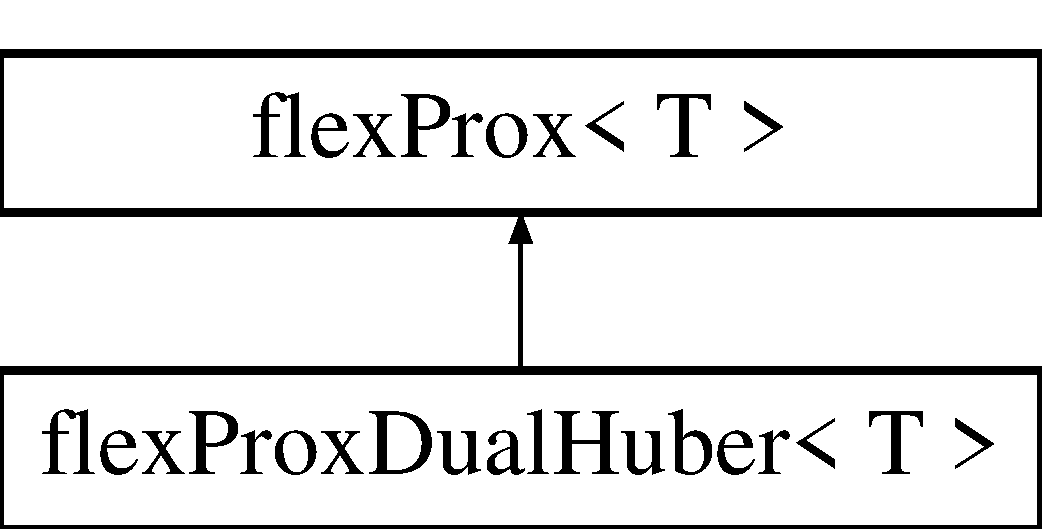
\includegraphics[height=2.000000cm]{classflex_prox_dual_huber}
\end{center}
\end{figure}
\subsection*{Classes}
\begin{DoxyCompactItemize}
\item 
struct {\bfseries flex\+Prox\+Dual\+Huber\+Dim2\+Functor}
\item 
struct {\bfseries flex\+Prox\+Dual\+Huber\+Dim3\+Functor}
\end{DoxyCompactItemize}
\subsection*{Public Member Functions}
\begin{DoxyCompactItemize}
\item 
\hyperlink{classflex_prox_dual_huber_a4ab9fe05ffc64193bb7150cad6525610}{flex\+Prox\+Dual\+Huber} (T a\+Huber\+Epsilon)
\begin{DoxyCompactList}\small\item\em initializes the Huber prox \end{DoxyCompactList}\item 
void \hyperlink{classflex_prox_dual_huber_af1e80a4361cda51e2b51aceeb69c6b79}{apply\+Prox} (T alpha, \hyperlink{classflex_box_data}{flex\+Box\+Data}$<$ T $>$ $\ast$data, const std\+::vector$<$ int $>$ \&dual\+Numbers, const std\+::vector$<$ int $>$ \&primal\+Numbers)
\begin{DoxyCompactList}\small\item\em applies prox for non-\/data terms \end{DoxyCompactList}\item 
void \hyperlink{classflex_prox_dual_huber_a4ce1a386510236fb80213dec59430ac4}{apply\+Prox} (T alpha, \hyperlink{classflex_box_data}{flex\+Box\+Data}$<$ T $>$ $\ast$data, const std\+::vector$<$ int $>$ \&dual\+Numbers, const std\+::vector$<$ int $>$ \&primal\+Numbers, std\+::vector$<$ Tdata $>$ \&f\+List)
\begin{DoxyCompactList}\small\item\em applies prox for data terms \end{DoxyCompactList}\end{DoxyCompactItemize}
\subsection*{Additional Inherited Members}


\subsection{Detailed Description}
\subsubsection*{template$<$typename T$>$\newline
class flex\+Prox\+Dual\+Huber$<$ T $>$}

represents prox for a Huber term 

$ \alpha \|\cdot\|_{H_\epsilon} $ 

\subsection{Constructor \& Destructor Documentation}
\mbox{\Hypertarget{classflex_prox_dual_huber_a4ab9fe05ffc64193bb7150cad6525610}\label{classflex_prox_dual_huber_a4ab9fe05ffc64193bb7150cad6525610}} 
\index{flex\+Prox\+Dual\+Huber@{flex\+Prox\+Dual\+Huber}!flex\+Prox\+Dual\+Huber@{flex\+Prox\+Dual\+Huber}}
\index{flex\+Prox\+Dual\+Huber@{flex\+Prox\+Dual\+Huber}!flex\+Prox\+Dual\+Huber@{flex\+Prox\+Dual\+Huber}}
\subsubsection{\texorpdfstring{flex\+Prox\+Dual\+Huber()}{flexProxDualHuber()}}
{\footnotesize\ttfamily template$<$typename T $>$ \\
\hyperlink{classflex_prox_dual_huber}{flex\+Prox\+Dual\+Huber}$<$ T $>$\+::\hyperlink{classflex_prox_dual_huber}{flex\+Prox\+Dual\+Huber} (\begin{DoxyParamCaption}\item[{T}]{a\+Huber\+Epsilon }\end{DoxyParamCaption})\hspace{0.3cm}{\ttfamily [inline]}}



initializes the Huber prox 


\begin{DoxyParams}{Parameters}
{\em a\+Huber\+Epsilon} & represents the parameter of the Huber norm (equals $ H_\epsilon $) \\
\hline
\end{DoxyParams}


\subsection{Member Function Documentation}
\mbox{\Hypertarget{classflex_prox_dual_huber_af1e80a4361cda51e2b51aceeb69c6b79}\label{classflex_prox_dual_huber_af1e80a4361cda51e2b51aceeb69c6b79}} 
\index{flex\+Prox\+Dual\+Huber@{flex\+Prox\+Dual\+Huber}!apply\+Prox@{apply\+Prox}}
\index{apply\+Prox@{apply\+Prox}!flex\+Prox\+Dual\+Huber@{flex\+Prox\+Dual\+Huber}}
\subsubsection{\texorpdfstring{apply\+Prox()}{applyProx()}\hspace{0.1cm}{\footnotesize\ttfamily [1/2]}}
{\footnotesize\ttfamily template$<$typename T $>$ \\
void \hyperlink{classflex_prox_dual_huber}{flex\+Prox\+Dual\+Huber}$<$ T $>$\+::apply\+Prox (\begin{DoxyParamCaption}\item[{T}]{alpha,  }\item[{\hyperlink{classflex_box_data}{flex\+Box\+Data}$<$ T $>$ $\ast$}]{data,  }\item[{const std\+::vector$<$ int $>$ \&}]{dual\+Numbers,  }\item[{const std\+::vector$<$ int $>$ \&}]{primal\+Numbers }\end{DoxyParamCaption})\hspace{0.3cm}{\ttfamily [inline]}, {\ttfamily [virtual]}}



applies prox for non-\/data terms 

the function body should be empty if implemented prox is a data prox 
\begin{DoxyParams}{Parameters}
{\em alpha} & weight of term \\
\hline
{\em data} & data object \\
\hline
{\em dual\+Numbers} & vector of internal identifactions of dual numbers corresponding to the term \\
\hline
\end{DoxyParams}
\begin{DoxySeeAlso}{See also}
\hyperlink{classflex_box}{flex\+Box} 
\end{DoxySeeAlso}

\begin{DoxyParams}{Parameters}
{\em primal\+Numbers} & vector of internal identifactions of primal numbers corresponding to the term \\
\hline
\end{DoxyParams}
\begin{DoxySeeAlso}{See also}
\hyperlink{classflex_box}{flex\+Box} 
\end{DoxySeeAlso}


Implements \hyperlink{classflex_prox_a6d3119bd368c4216ad264a1f6dc1d01f}{flex\+Prox$<$ T $>$}.

\mbox{\Hypertarget{classflex_prox_dual_huber_a4ce1a386510236fb80213dec59430ac4}\label{classflex_prox_dual_huber_a4ce1a386510236fb80213dec59430ac4}} 
\index{flex\+Prox\+Dual\+Huber@{flex\+Prox\+Dual\+Huber}!apply\+Prox@{apply\+Prox}}
\index{apply\+Prox@{apply\+Prox}!flex\+Prox\+Dual\+Huber@{flex\+Prox\+Dual\+Huber}}
\subsubsection{\texorpdfstring{apply\+Prox()}{applyProx()}\hspace{0.1cm}{\footnotesize\ttfamily [2/2]}}
{\footnotesize\ttfamily template$<$typename T $>$ \\
void \hyperlink{classflex_prox_dual_huber}{flex\+Prox\+Dual\+Huber}$<$ T $>$\+::apply\+Prox (\begin{DoxyParamCaption}\item[{T}]{alpha,  }\item[{\hyperlink{classflex_box_data}{flex\+Box\+Data}$<$ T $>$ $\ast$}]{data,  }\item[{const std\+::vector$<$ int $>$ \&}]{dual\+Numbers,  }\item[{const std\+::vector$<$ int $>$ \&}]{primal\+Numbers,  }\item[{std\+::vector$<$ Tdata $>$ \&}]{f\+List }\end{DoxyParamCaption})\hspace{0.3cm}{\ttfamily [inline]}, {\ttfamily [virtual]}}



applies prox for data terms 

the function body should be empty if implemented prox is a non-\/data prox 
\begin{DoxyParams}{Parameters}
{\em alpha} & weight of term \\
\hline
{\em data} & data object \\
\hline
{\em dual\+Numbers} & vector of internal identifactions of dual numbers corresponding to the term \\
\hline
\end{DoxyParams}
\begin{DoxySeeAlso}{See also}
\hyperlink{classflex_box}{flex\+Box} 
\end{DoxySeeAlso}

\begin{DoxyParams}{Parameters}
{\em primal\+Numbers} & vector of internal identifactions of primal numbers corresponding to the term \\
\hline
\end{DoxyParams}
\begin{DoxySeeAlso}{See also}
\hyperlink{classflex_box}{flex\+Box} 
\end{DoxySeeAlso}

\begin{DoxyParams}{Parameters}
{\em f\+List} & data part of term \\
\hline
\end{DoxyParams}


Implements \hyperlink{classflex_prox_aec433ffbf1a7586f26a2116c6b94bdd6}{flex\+Prox$<$ T $>$}.



The documentation for this class was generated from the following file\+:\begin{DoxyCompactItemize}
\item 
flex\+Prox\+Dual\+Huber.\+h\end{DoxyCompactItemize}

\hypertarget{classflex_prox_dual_inner_product}{}\section{flex\+Prox\+Dual\+Inner\+Product$<$ T $>$ Class Template Reference}
\label{classflex_prox_dual_inner_product}\index{flex\+Prox\+Dual\+Inner\+Product$<$ T $>$@{flex\+Prox\+Dual\+Inner\+Product$<$ T $>$}}


represents prox for an inner product data term  




{\ttfamily \#include $<$flex\+Prox\+Dual\+Inner\+Product.\+h$>$}

Inheritance diagram for flex\+Prox\+Dual\+Inner\+Product$<$ T $>$\+:\begin{figure}[H]
\begin{center}
\leavevmode
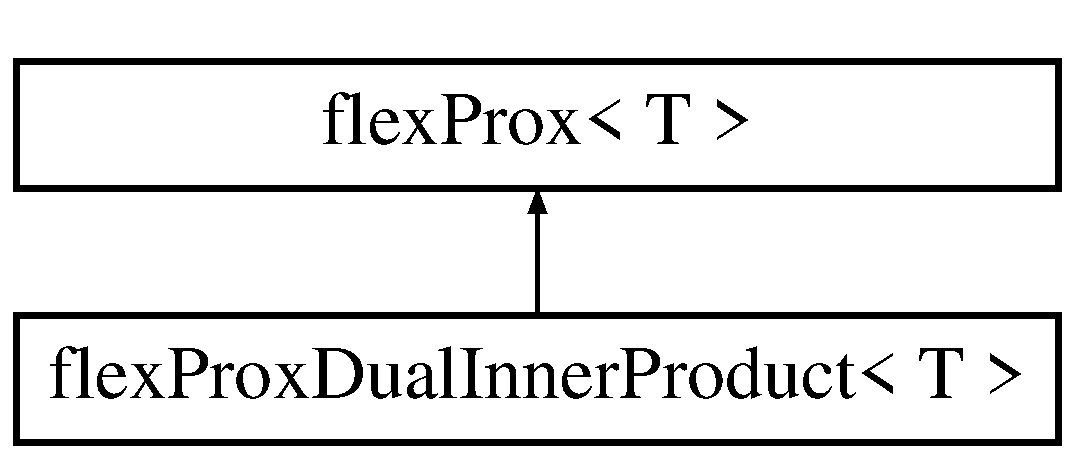
\includegraphics[height=2.000000cm]{classflex_prox_dual_inner_product}
\end{center}
\end{figure}
\subsection*{Public Member Functions}
\begin{DoxyCompactItemize}
\item 
void \hyperlink{classflex_prox_dual_inner_product_ac12298c520f5e8e81724e330e8dae6a3}{apply\+Prox} (T alpha, \hyperlink{classflex_box_data}{flex\+Box\+Data}$<$ T $>$ $\ast$data, const std\+::vector$<$ int $>$ \&dual\+Numbers, const std\+::vector$<$ int $>$ \&primal\+Numbers)
\begin{DoxyCompactList}\small\item\em applies prox for non-\/data terms \end{DoxyCompactList}\item 
void \hyperlink{classflex_prox_dual_inner_product_aa2444bfc4ad1c4ce77e9204bd9f85f69}{apply\+Prox} (T alpha, \hyperlink{classflex_box_data}{flex\+Box\+Data}$<$ T $>$ $\ast$data, const std\+::vector$<$ int $>$ \&dual\+Numbers, const std\+::vector$<$ int $>$ \&primal\+Numbers, std\+::vector$<$ Tdata $>$ \&f\+List)
\begin{DoxyCompactList}\small\item\em applies prox for data terms \end{DoxyCompactList}\end{DoxyCompactItemize}
\subsection*{Additional Inherited Members}


\subsection{Detailed Description}
\subsubsection*{template$<$typename T$>$\newline
class flex\+Prox\+Dual\+Inner\+Product$<$ T $>$}

represents prox for an inner product data term 

$ \alpha \langle \cdot,f\rangle $ 

\subsection{Member Function Documentation}
\mbox{\Hypertarget{classflex_prox_dual_inner_product_ac12298c520f5e8e81724e330e8dae6a3}\label{classflex_prox_dual_inner_product_ac12298c520f5e8e81724e330e8dae6a3}} 
\index{flex\+Prox\+Dual\+Inner\+Product@{flex\+Prox\+Dual\+Inner\+Product}!apply\+Prox@{apply\+Prox}}
\index{apply\+Prox@{apply\+Prox}!flex\+Prox\+Dual\+Inner\+Product@{flex\+Prox\+Dual\+Inner\+Product}}
\subsubsection{\texorpdfstring{apply\+Prox()}{applyProx()}\hspace{0.1cm}{\footnotesize\ttfamily [1/2]}}
{\footnotesize\ttfamily template$<$typename T $>$ \\
void \hyperlink{classflex_prox_dual_inner_product}{flex\+Prox\+Dual\+Inner\+Product}$<$ T $>$\+::apply\+Prox (\begin{DoxyParamCaption}\item[{T}]{alpha,  }\item[{\hyperlink{classflex_box_data}{flex\+Box\+Data}$<$ T $>$ $\ast$}]{data,  }\item[{const std\+::vector$<$ int $>$ \&}]{dual\+Numbers,  }\item[{const std\+::vector$<$ int $>$ \&}]{primal\+Numbers }\end{DoxyParamCaption})\hspace{0.3cm}{\ttfamily [inline]}, {\ttfamily [virtual]}}



applies prox for non-\/data terms 

the function body should be empty if implemented prox is a data prox 
\begin{DoxyParams}{Parameters}
{\em alpha} & weight of term \\
\hline
{\em data} & data object \\
\hline
{\em dual\+Numbers} & vector of internal identifactions of dual numbers corresponding to the term \\
\hline
\end{DoxyParams}
\begin{DoxySeeAlso}{See also}
\hyperlink{classflex_box}{flex\+Box} 
\end{DoxySeeAlso}

\begin{DoxyParams}{Parameters}
{\em primal\+Numbers} & vector of internal identifactions of primal numbers corresponding to the term \\
\hline
\end{DoxyParams}
\begin{DoxySeeAlso}{See also}
\hyperlink{classflex_box}{flex\+Box} 
\end{DoxySeeAlso}


Implements \hyperlink{classflex_prox_a6d3119bd368c4216ad264a1f6dc1d01f}{flex\+Prox$<$ T $>$}.

\mbox{\Hypertarget{classflex_prox_dual_inner_product_aa2444bfc4ad1c4ce77e9204bd9f85f69}\label{classflex_prox_dual_inner_product_aa2444bfc4ad1c4ce77e9204bd9f85f69}} 
\index{flex\+Prox\+Dual\+Inner\+Product@{flex\+Prox\+Dual\+Inner\+Product}!apply\+Prox@{apply\+Prox}}
\index{apply\+Prox@{apply\+Prox}!flex\+Prox\+Dual\+Inner\+Product@{flex\+Prox\+Dual\+Inner\+Product}}
\subsubsection{\texorpdfstring{apply\+Prox()}{applyProx()}\hspace{0.1cm}{\footnotesize\ttfamily [2/2]}}
{\footnotesize\ttfamily template$<$typename T $>$ \\
void \hyperlink{classflex_prox_dual_inner_product}{flex\+Prox\+Dual\+Inner\+Product}$<$ T $>$\+::apply\+Prox (\begin{DoxyParamCaption}\item[{T}]{alpha,  }\item[{\hyperlink{classflex_box_data}{flex\+Box\+Data}$<$ T $>$ $\ast$}]{data,  }\item[{const std\+::vector$<$ int $>$ \&}]{dual\+Numbers,  }\item[{const std\+::vector$<$ int $>$ \&}]{primal\+Numbers,  }\item[{std\+::vector$<$ Tdata $>$ \&}]{f\+List }\end{DoxyParamCaption})\hspace{0.3cm}{\ttfamily [inline]}, {\ttfamily [virtual]}}



applies prox for data terms 

the function body should be empty if implemented prox is a non-\/data prox 
\begin{DoxyParams}{Parameters}
{\em alpha} & weight of term \\
\hline
{\em data} & data object \\
\hline
{\em dual\+Numbers} & vector of internal identifactions of dual numbers corresponding to the term \\
\hline
\end{DoxyParams}
\begin{DoxySeeAlso}{See also}
\hyperlink{classflex_box}{flex\+Box} 
\end{DoxySeeAlso}

\begin{DoxyParams}{Parameters}
{\em primal\+Numbers} & vector of internal identifactions of primal numbers corresponding to the term \\
\hline
\end{DoxyParams}
\begin{DoxySeeAlso}{See also}
\hyperlink{classflex_box}{flex\+Box} 
\end{DoxySeeAlso}

\begin{DoxyParams}{Parameters}
{\em f\+List} & data part of term \\
\hline
\end{DoxyParams}


Implements \hyperlink{classflex_prox_aec433ffbf1a7586f26a2116c6b94bdd6}{flex\+Prox$<$ T $>$}.



The documentation for this class was generated from the following file\+:\begin{DoxyCompactItemize}
\item 
flex\+Prox\+Dual\+Inner\+Product.\+h\end{DoxyCompactItemize}

\hypertarget{classflex_prox_dual_l1_aniso}{}\section{flex\+Prox\+Dual\+L1\+Aniso$<$ T $>$ Class Template Reference}
\label{classflex_prox_dual_l1_aniso}\index{flex\+Prox\+Dual\+L1\+Aniso$<$ T $>$@{flex\+Prox\+Dual\+L1\+Aniso$<$ T $>$}}


represents prox for a L1 non-\/data term  




{\ttfamily \#include $<$flex\+Prox\+Dual\+L1\+Aniso.\+h$>$}

Inheritance diagram for flex\+Prox\+Dual\+L1\+Aniso$<$ T $>$\+:\begin{figure}[H]
\begin{center}
\leavevmode
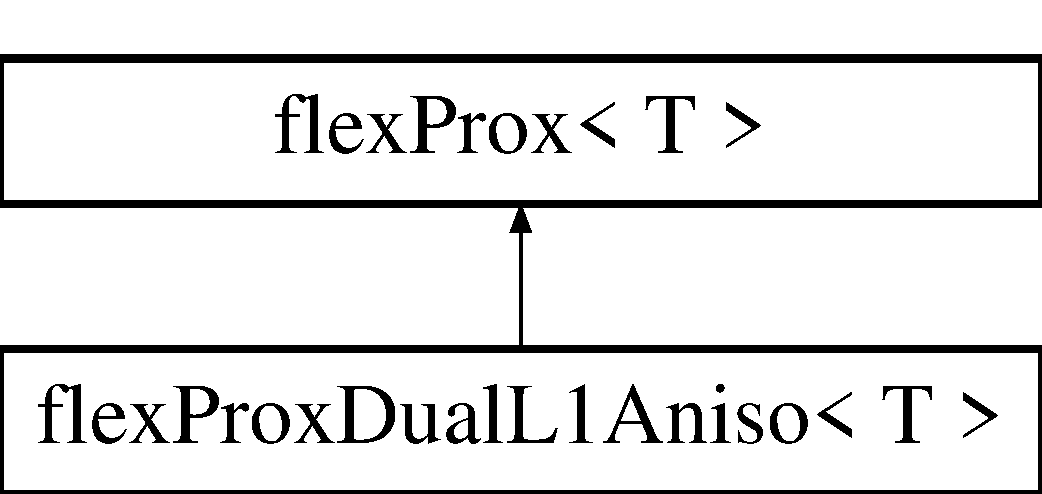
\includegraphics[height=2.000000cm]{classflex_prox_dual_l1_aniso}
\end{center}
\end{figure}
\subsection*{Classes}
\begin{DoxyCompactItemize}
\item 
struct {\bfseries flex\+Prox\+Dual\+L1\+Aniso\+Functor}
\end{DoxyCompactItemize}
\subsection*{Public Member Functions}
\begin{DoxyCompactItemize}
\item 
void \hyperlink{classflex_prox_dual_l1_aniso_afef01f75247ba5a8990c5b77a7ab89f0}{apply\+Prox} (T alpha, \hyperlink{classflex_box_data}{flex\+Box\+Data}$<$ T $>$ $\ast$data, const std\+::vector$<$ int $>$ \&dual\+Numbers, const std\+::vector$<$ int $>$ \&primal\+Numbers)
\begin{DoxyCompactList}\small\item\em applies prox for non-\/data terms \end{DoxyCompactList}\item 
void \hyperlink{classflex_prox_dual_l1_aniso_aff8e46fb892387898d54516f0df3c080}{apply\+Prox} (T alpha, \hyperlink{classflex_box_data}{flex\+Box\+Data}$<$ T $>$ $\ast$data, const std\+::vector$<$ int $>$ \&dual\+Numbers, const std\+::vector$<$ int $>$ \&primal\+Numbers, std\+::vector$<$ Tdata $>$ \&f\+List)
\begin{DoxyCompactList}\small\item\em applies prox for data terms \end{DoxyCompactList}\end{DoxyCompactItemize}
\subsection*{Additional Inherited Members}


\subsection{Detailed Description}
\subsubsection*{template$<$typename T$>$\newline
class flex\+Prox\+Dual\+L1\+Aniso$<$ T $>$}

represents prox for a L1 non-\/data term 

$ \alpha \|\cdot\|_{1,1} $ 

\subsection{Member Function Documentation}
\mbox{\Hypertarget{classflex_prox_dual_l1_aniso_afef01f75247ba5a8990c5b77a7ab89f0}\label{classflex_prox_dual_l1_aniso_afef01f75247ba5a8990c5b77a7ab89f0}} 
\index{flex\+Prox\+Dual\+L1\+Aniso@{flex\+Prox\+Dual\+L1\+Aniso}!apply\+Prox@{apply\+Prox}}
\index{apply\+Prox@{apply\+Prox}!flex\+Prox\+Dual\+L1\+Aniso@{flex\+Prox\+Dual\+L1\+Aniso}}
\subsubsection{\texorpdfstring{apply\+Prox()}{applyProx()}\hspace{0.1cm}{\footnotesize\ttfamily [1/2]}}
{\footnotesize\ttfamily template$<$typename T $>$ \\
void \hyperlink{classflex_prox_dual_l1_aniso}{flex\+Prox\+Dual\+L1\+Aniso}$<$ T $>$\+::apply\+Prox (\begin{DoxyParamCaption}\item[{T}]{alpha,  }\item[{\hyperlink{classflex_box_data}{flex\+Box\+Data}$<$ T $>$ $\ast$}]{data,  }\item[{const std\+::vector$<$ int $>$ \&}]{dual\+Numbers,  }\item[{const std\+::vector$<$ int $>$ \&}]{primal\+Numbers }\end{DoxyParamCaption})\hspace{0.3cm}{\ttfamily [inline]}, {\ttfamily [virtual]}}



applies prox for non-\/data terms 

the function body should be empty if implemented prox is a data prox 
\begin{DoxyParams}{Parameters}
{\em alpha} & weight of term \\
\hline
{\em data} & data object \\
\hline
{\em dual\+Numbers} & vector of internal identifactions of dual numbers corresponding to the term \\
\hline
\end{DoxyParams}
\begin{DoxySeeAlso}{See also}
\hyperlink{classflex_box}{flex\+Box} 
\end{DoxySeeAlso}

\begin{DoxyParams}{Parameters}
{\em primal\+Numbers} & vector of internal identifactions of primal numbers corresponding to the term \\
\hline
\end{DoxyParams}
\begin{DoxySeeAlso}{See also}
\hyperlink{classflex_box}{flex\+Box} 
\end{DoxySeeAlso}


Implements \hyperlink{classflex_prox_a6d3119bd368c4216ad264a1f6dc1d01f}{flex\+Prox$<$ T $>$}.

\mbox{\Hypertarget{classflex_prox_dual_l1_aniso_aff8e46fb892387898d54516f0df3c080}\label{classflex_prox_dual_l1_aniso_aff8e46fb892387898d54516f0df3c080}} 
\index{flex\+Prox\+Dual\+L1\+Aniso@{flex\+Prox\+Dual\+L1\+Aniso}!apply\+Prox@{apply\+Prox}}
\index{apply\+Prox@{apply\+Prox}!flex\+Prox\+Dual\+L1\+Aniso@{flex\+Prox\+Dual\+L1\+Aniso}}
\subsubsection{\texorpdfstring{apply\+Prox()}{applyProx()}\hspace{0.1cm}{\footnotesize\ttfamily [2/2]}}
{\footnotesize\ttfamily template$<$typename T $>$ \\
void \hyperlink{classflex_prox_dual_l1_aniso}{flex\+Prox\+Dual\+L1\+Aniso}$<$ T $>$\+::apply\+Prox (\begin{DoxyParamCaption}\item[{T}]{alpha,  }\item[{\hyperlink{classflex_box_data}{flex\+Box\+Data}$<$ T $>$ $\ast$}]{data,  }\item[{const std\+::vector$<$ int $>$ \&}]{dual\+Numbers,  }\item[{const std\+::vector$<$ int $>$ \&}]{primal\+Numbers,  }\item[{std\+::vector$<$ Tdata $>$ \&}]{f\+List }\end{DoxyParamCaption})\hspace{0.3cm}{\ttfamily [inline]}, {\ttfamily [virtual]}}



applies prox for data terms 

the function body should be empty if implemented prox is a non-\/data prox 
\begin{DoxyParams}{Parameters}
{\em alpha} & weight of term \\
\hline
{\em data} & data object \\
\hline
{\em dual\+Numbers} & vector of internal identifactions of dual numbers corresponding to the term \\
\hline
\end{DoxyParams}
\begin{DoxySeeAlso}{See also}
\hyperlink{classflex_box}{flex\+Box} 
\end{DoxySeeAlso}

\begin{DoxyParams}{Parameters}
{\em primal\+Numbers} & vector of internal identifactions of primal numbers corresponding to the term \\
\hline
\end{DoxyParams}
\begin{DoxySeeAlso}{See also}
\hyperlink{classflex_box}{flex\+Box} 
\end{DoxySeeAlso}

\begin{DoxyParams}{Parameters}
{\em f\+List} & data part of term \\
\hline
\end{DoxyParams}


Implements \hyperlink{classflex_prox_aec433ffbf1a7586f26a2116c6b94bdd6}{flex\+Prox$<$ T $>$}.



The documentation for this class was generated from the following file\+:\begin{DoxyCompactItemize}
\item 
flex\+Prox\+Dual\+L1\+Aniso.\+h\end{DoxyCompactItemize}

\hypertarget{classflex_prox_dual_l1_iso}{}\section{flex\+Prox\+Dual\+L1\+Iso$<$ T $>$ Class Template Reference}
\label{classflex_prox_dual_l1_iso}\index{flex\+Prox\+Dual\+L1\+Iso$<$ T $>$@{flex\+Prox\+Dual\+L1\+Iso$<$ T $>$}}


represents prox for a L1 non-\/data term  




{\ttfamily \#include $<$flex\+Prox\+Dual\+L1\+Iso.\+h$>$}

Inheritance diagram for flex\+Prox\+Dual\+L1\+Iso$<$ T $>$\+:\begin{figure}[H]
\begin{center}
\leavevmode
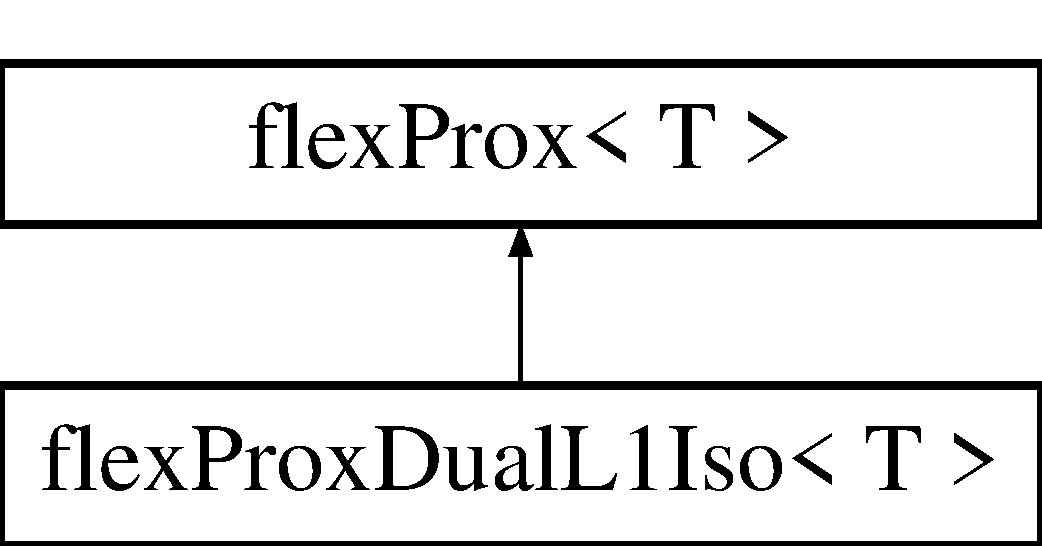
\includegraphics[height=2.000000cm]{classflex_prox_dual_l1_iso}
\end{center}
\end{figure}
\subsection*{Classes}
\begin{DoxyCompactItemize}
\item 
struct {\bfseries flex\+Prox\+Dual\+L1\+Iso\+Dim1\+Functor}
\item 
struct {\bfseries flex\+Prox\+Dual\+L1\+Iso\+Dim2\+Functor}
\item 
struct {\bfseries flex\+Prox\+Dual\+L1\+Iso\+Dim3\+Functor}
\end{DoxyCompactItemize}
\subsection*{Public Member Functions}
\begin{DoxyCompactItemize}
\item 
void \hyperlink{classflex_prox_dual_l1_iso_afbf9d355a5c633355233f6b7d6026465}{apply\+Prox} (T alpha, \hyperlink{classflex_box_data}{flex\+Box\+Data}$<$ T $>$ $\ast$data, const std\+::vector$<$ int $>$ \&dual\+Numbers, const std\+::vector$<$ int $>$ \&primal\+Numbers)
\begin{DoxyCompactList}\small\item\em applies prox for non-\/data terms \end{DoxyCompactList}\item 
void \hyperlink{classflex_prox_dual_l1_iso_a5cd236c5d3e58b9424b1021694c44590}{apply\+Prox} (T alpha, \hyperlink{classflex_box_data}{flex\+Box\+Data}$<$ T $>$ $\ast$data, const std\+::vector$<$ int $>$ \&dual\+Numbers, const std\+::vector$<$ int $>$ \&primal\+Numbers, std\+::vector$<$ Tdata $>$ \&f\+List)
\begin{DoxyCompactList}\small\item\em applies prox for data terms \end{DoxyCompactList}\end{DoxyCompactItemize}
\subsection*{Additional Inherited Members}


\subsection{Detailed Description}
\subsubsection*{template$<$typename T$>$\newline
class flex\+Prox\+Dual\+L1\+Iso$<$ T $>$}

represents prox for a L1 non-\/data term 

$ \alpha \|\cdot\|_{2,1} $ 

\subsection{Member Function Documentation}
\mbox{\Hypertarget{classflex_prox_dual_l1_iso_afbf9d355a5c633355233f6b7d6026465}\label{classflex_prox_dual_l1_iso_afbf9d355a5c633355233f6b7d6026465}} 
\index{flex\+Prox\+Dual\+L1\+Iso@{flex\+Prox\+Dual\+L1\+Iso}!apply\+Prox@{apply\+Prox}}
\index{apply\+Prox@{apply\+Prox}!flex\+Prox\+Dual\+L1\+Iso@{flex\+Prox\+Dual\+L1\+Iso}}
\subsubsection{\texorpdfstring{apply\+Prox()}{applyProx()}\hspace{0.1cm}{\footnotesize\ttfamily [1/2]}}
{\footnotesize\ttfamily template$<$typename T $>$ \\
void \hyperlink{classflex_prox_dual_l1_iso}{flex\+Prox\+Dual\+L1\+Iso}$<$ T $>$\+::apply\+Prox (\begin{DoxyParamCaption}\item[{T}]{alpha,  }\item[{\hyperlink{classflex_box_data}{flex\+Box\+Data}$<$ T $>$ $\ast$}]{data,  }\item[{const std\+::vector$<$ int $>$ \&}]{dual\+Numbers,  }\item[{const std\+::vector$<$ int $>$ \&}]{primal\+Numbers }\end{DoxyParamCaption})\hspace{0.3cm}{\ttfamily [inline]}, {\ttfamily [virtual]}}



applies prox for non-\/data terms 

the function body should be empty if implemented prox is a data prox 
\begin{DoxyParams}{Parameters}
{\em alpha} & weight of term \\
\hline
{\em data} & data object \\
\hline
{\em dual\+Numbers} & vector of internal identifactions of dual numbers corresponding to the term \\
\hline
\end{DoxyParams}
\begin{DoxySeeAlso}{See also}
\hyperlink{classflex_box}{flex\+Box} 
\end{DoxySeeAlso}

\begin{DoxyParams}{Parameters}
{\em primal\+Numbers} & vector of internal identifactions of primal numbers corresponding to the term \\
\hline
\end{DoxyParams}
\begin{DoxySeeAlso}{See also}
\hyperlink{classflex_box}{flex\+Box} 
\end{DoxySeeAlso}


Implements \hyperlink{classflex_prox_a6d3119bd368c4216ad264a1f6dc1d01f}{flex\+Prox$<$ T $>$}.

\mbox{\Hypertarget{classflex_prox_dual_l1_iso_a5cd236c5d3e58b9424b1021694c44590}\label{classflex_prox_dual_l1_iso_a5cd236c5d3e58b9424b1021694c44590}} 
\index{flex\+Prox\+Dual\+L1\+Iso@{flex\+Prox\+Dual\+L1\+Iso}!apply\+Prox@{apply\+Prox}}
\index{apply\+Prox@{apply\+Prox}!flex\+Prox\+Dual\+L1\+Iso@{flex\+Prox\+Dual\+L1\+Iso}}
\subsubsection{\texorpdfstring{apply\+Prox()}{applyProx()}\hspace{0.1cm}{\footnotesize\ttfamily [2/2]}}
{\footnotesize\ttfamily template$<$typename T $>$ \\
void \hyperlink{classflex_prox_dual_l1_iso}{flex\+Prox\+Dual\+L1\+Iso}$<$ T $>$\+::apply\+Prox (\begin{DoxyParamCaption}\item[{T}]{alpha,  }\item[{\hyperlink{classflex_box_data}{flex\+Box\+Data}$<$ T $>$ $\ast$}]{data,  }\item[{const std\+::vector$<$ int $>$ \&}]{dual\+Numbers,  }\item[{const std\+::vector$<$ int $>$ \&}]{primal\+Numbers,  }\item[{std\+::vector$<$ Tdata $>$ \&}]{f\+List }\end{DoxyParamCaption})\hspace{0.3cm}{\ttfamily [inline]}, {\ttfamily [virtual]}}



applies prox for data terms 

the function body should be empty if implemented prox is a non-\/data prox 
\begin{DoxyParams}{Parameters}
{\em alpha} & weight of term \\
\hline
{\em data} & data object \\
\hline
{\em dual\+Numbers} & vector of internal identifactions of dual numbers corresponding to the term \\
\hline
\end{DoxyParams}
\begin{DoxySeeAlso}{See also}
\hyperlink{classflex_box}{flex\+Box} 
\end{DoxySeeAlso}

\begin{DoxyParams}{Parameters}
{\em primal\+Numbers} & vector of internal identifactions of primal numbers corresponding to the term \\
\hline
\end{DoxyParams}
\begin{DoxySeeAlso}{See also}
\hyperlink{classflex_box}{flex\+Box} 
\end{DoxySeeAlso}

\begin{DoxyParams}{Parameters}
{\em f\+List} & data part of term \\
\hline
\end{DoxyParams}


Implements \hyperlink{classflex_prox_aec433ffbf1a7586f26a2116c6b94bdd6}{flex\+Prox$<$ T $>$}.



The documentation for this class was generated from the following file\+:\begin{DoxyCompactItemize}
\item 
flex\+Prox\+Dual\+L1\+Iso.\+h\end{DoxyCompactItemize}

\hypertarget{classflex_prox_dual_l2}{}\section{flex\+Prox\+Dual\+L2$<$ T $>$ Class Template Reference}
\label{classflex_prox_dual_l2}\index{flex\+Prox\+Dual\+L2$<$ T $>$@{flex\+Prox\+Dual\+L2$<$ T $>$}}


represents prox for a L2 non-\/data term  




{\ttfamily \#include $<$flex\+Prox\+Dual\+L2.\+h$>$}

Inheritance diagram for flex\+Prox\+Dual\+L2$<$ T $>$\+:\begin{figure}[H]
\begin{center}
\leavevmode
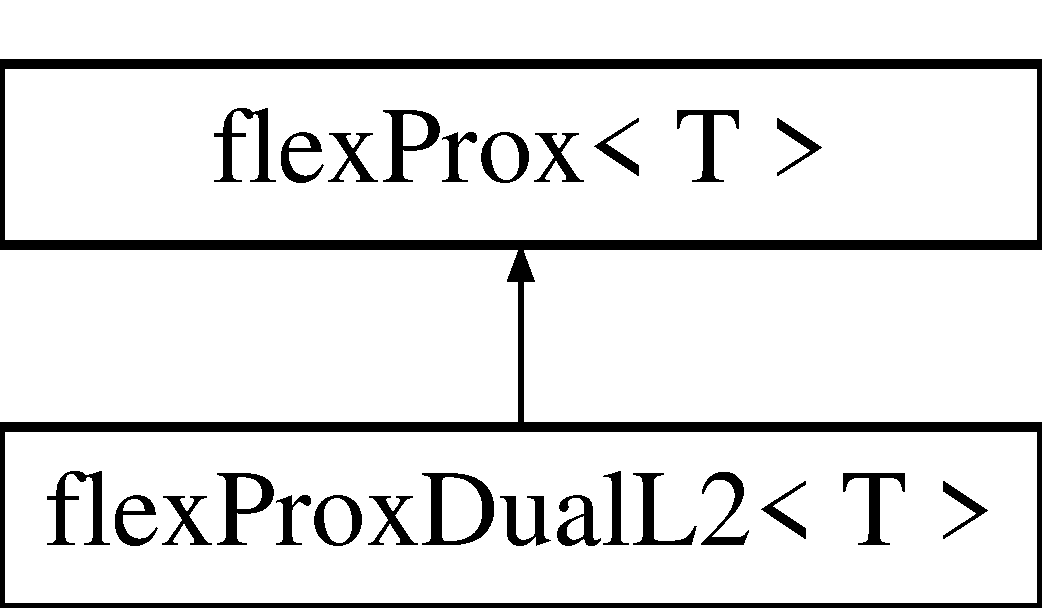
\includegraphics[height=2.000000cm]{classflex_prox_dual_l2}
\end{center}
\end{figure}
\subsection*{Classes}
\begin{DoxyCompactItemize}
\item 
struct {\bfseries flex\+Prox\+Dual\+L2\+Functor}
\end{DoxyCompactItemize}
\subsection*{Public Member Functions}
\begin{DoxyCompactItemize}
\item 
void \hyperlink{classflex_prox_dual_l2_ad4574da3855bad6596c8a3fda028c933}{apply\+Prox} (T alpha, \hyperlink{classflex_box_data}{flex\+Box\+Data}$<$ T $>$ $\ast$data, const std\+::vector$<$ int $>$ \&dual\+Numbers, const std\+::vector$<$ int $>$ \&primal\+Numbers)
\begin{DoxyCompactList}\small\item\em applies prox for non-\/data terms \end{DoxyCompactList}\item 
void \hyperlink{classflex_prox_dual_l2_aef49de69c4d5e6baafbecbab934c17ce}{apply\+Prox} (T alpha, \hyperlink{classflex_box_data}{flex\+Box\+Data}$<$ T $>$ $\ast$data, const std\+::vector$<$ int $>$ \&dual\+Numbers, const std\+::vector$<$ int $>$ \&primal\+Numbers, std\+::vector$<$ Tdata $>$ \&f\+List)
\begin{DoxyCompactList}\small\item\em applies prox for data terms \end{DoxyCompactList}\end{DoxyCompactItemize}
\subsection*{Additional Inherited Members}


\subsection{Detailed Description}
\subsubsection*{template$<$typename T$>$\newline
class flex\+Prox\+Dual\+L2$<$ T $>$}

represents prox for a L2 non-\/data term 

$ \frac{\alpha}{2} \|\cdot\|_2^2 $ 

\subsection{Member Function Documentation}
\mbox{\Hypertarget{classflex_prox_dual_l2_ad4574da3855bad6596c8a3fda028c933}\label{classflex_prox_dual_l2_ad4574da3855bad6596c8a3fda028c933}} 
\index{flex\+Prox\+Dual\+L2@{flex\+Prox\+Dual\+L2}!apply\+Prox@{apply\+Prox}}
\index{apply\+Prox@{apply\+Prox}!flex\+Prox\+Dual\+L2@{flex\+Prox\+Dual\+L2}}
\subsubsection{\texorpdfstring{apply\+Prox()}{applyProx()}\hspace{0.1cm}{\footnotesize\ttfamily [1/2]}}
{\footnotesize\ttfamily template$<$typename T $>$ \\
void \hyperlink{classflex_prox_dual_l2}{flex\+Prox\+Dual\+L2}$<$ T $>$\+::apply\+Prox (\begin{DoxyParamCaption}\item[{T}]{alpha,  }\item[{\hyperlink{classflex_box_data}{flex\+Box\+Data}$<$ T $>$ $\ast$}]{data,  }\item[{const std\+::vector$<$ int $>$ \&}]{dual\+Numbers,  }\item[{const std\+::vector$<$ int $>$ \&}]{primal\+Numbers }\end{DoxyParamCaption})\hspace{0.3cm}{\ttfamily [inline]}, {\ttfamily [virtual]}}



applies prox for non-\/data terms 

the function body should be empty if implemented prox is a data prox 
\begin{DoxyParams}{Parameters}
{\em alpha} & weight of term \\
\hline
{\em data} & data object \\
\hline
{\em dual\+Numbers} & vector of internal identifactions of dual numbers corresponding to the term \\
\hline
\end{DoxyParams}
\begin{DoxySeeAlso}{See also}
\hyperlink{classflex_box}{flex\+Box} 
\end{DoxySeeAlso}

\begin{DoxyParams}{Parameters}
{\em primal\+Numbers} & vector of internal identifactions of primal numbers corresponding to the term \\
\hline
\end{DoxyParams}
\begin{DoxySeeAlso}{See also}
\hyperlink{classflex_box}{flex\+Box} 
\end{DoxySeeAlso}


Implements \hyperlink{classflex_prox_a6d3119bd368c4216ad264a1f6dc1d01f}{flex\+Prox$<$ T $>$}.

\mbox{\Hypertarget{classflex_prox_dual_l2_aef49de69c4d5e6baafbecbab934c17ce}\label{classflex_prox_dual_l2_aef49de69c4d5e6baafbecbab934c17ce}} 
\index{flex\+Prox\+Dual\+L2@{flex\+Prox\+Dual\+L2}!apply\+Prox@{apply\+Prox}}
\index{apply\+Prox@{apply\+Prox}!flex\+Prox\+Dual\+L2@{flex\+Prox\+Dual\+L2}}
\subsubsection{\texorpdfstring{apply\+Prox()}{applyProx()}\hspace{0.1cm}{\footnotesize\ttfamily [2/2]}}
{\footnotesize\ttfamily template$<$typename T $>$ \\
void \hyperlink{classflex_prox_dual_l2}{flex\+Prox\+Dual\+L2}$<$ T $>$\+::apply\+Prox (\begin{DoxyParamCaption}\item[{T}]{alpha,  }\item[{\hyperlink{classflex_box_data}{flex\+Box\+Data}$<$ T $>$ $\ast$}]{data,  }\item[{const std\+::vector$<$ int $>$ \&}]{dual\+Numbers,  }\item[{const std\+::vector$<$ int $>$ \&}]{primal\+Numbers,  }\item[{std\+::vector$<$ Tdata $>$ \&}]{f\+List }\end{DoxyParamCaption})\hspace{0.3cm}{\ttfamily [inline]}, {\ttfamily [virtual]}}



applies prox for data terms 

the function body should be empty if implemented prox is a non-\/data prox 
\begin{DoxyParams}{Parameters}
{\em alpha} & weight of term \\
\hline
{\em data} & data object \\
\hline
{\em dual\+Numbers} & vector of internal identifactions of dual numbers corresponding to the term \\
\hline
\end{DoxyParams}
\begin{DoxySeeAlso}{See also}
\hyperlink{classflex_box}{flex\+Box} 
\end{DoxySeeAlso}

\begin{DoxyParams}{Parameters}
{\em primal\+Numbers} & vector of internal identifactions of primal numbers corresponding to the term \\
\hline
\end{DoxyParams}
\begin{DoxySeeAlso}{See also}
\hyperlink{classflex_box}{flex\+Box} 
\end{DoxySeeAlso}

\begin{DoxyParams}{Parameters}
{\em f\+List} & data part of term \\
\hline
\end{DoxyParams}


Implements \hyperlink{classflex_prox_aec433ffbf1a7586f26a2116c6b94bdd6}{flex\+Prox$<$ T $>$}.



The documentation for this class was generated from the following file\+:\begin{DoxyCompactItemize}
\item 
flex\+Prox\+Dual\+L2.\+h\end{DoxyCompactItemize}

\hypertarget{classflex_prox_dual_l2_inf}{}\section{flex\+Prox\+Dual\+L2\+Inf$<$ T $>$ Class Template Reference}
\label{classflex_prox_dual_l2_inf}\index{flex\+Prox\+Dual\+L2\+Inf$<$ T $>$@{flex\+Prox\+Dual\+L2\+Inf$<$ T $>$}}


represents prox for a L2,inf non-\/data term  




{\ttfamily \#include $<$flex\+Prox\+Dual\+L2\+Inf.\+h$>$}

Inheritance diagram for flex\+Prox\+Dual\+L2\+Inf$<$ T $>$\+:\begin{figure}[H]
\begin{center}
\leavevmode
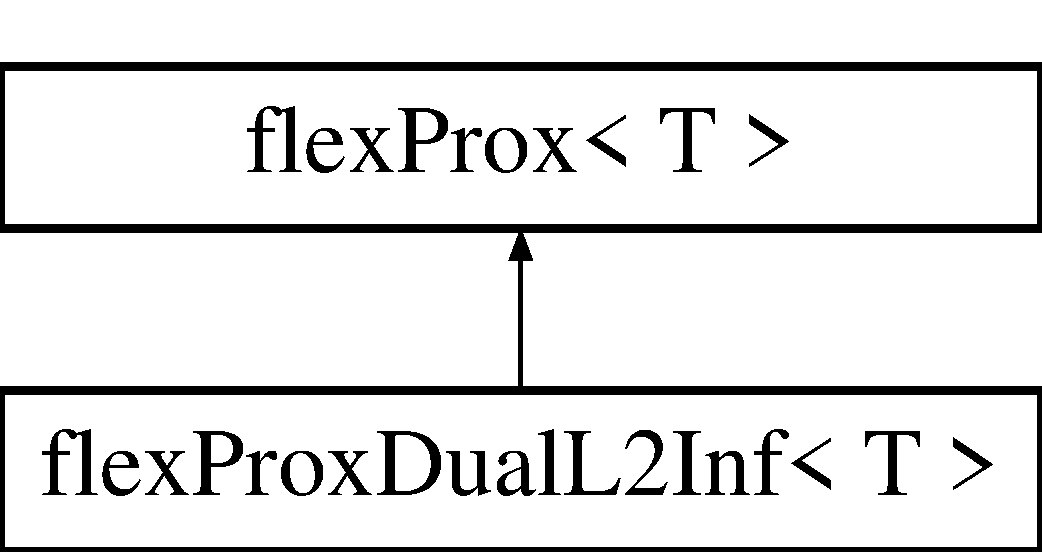
\includegraphics[height=2.000000cm]{classflex_prox_dual_l2_inf}
\end{center}
\end{figure}
\subsection*{Classes}
\begin{DoxyCompactItemize}
\item 
struct {\bfseries Abs\+Functor}
\item 
struct \hyperlink{structflex_prox_dual_l2_inf_1_1_find_transform}{Find\+Transform}
\item 
struct \hyperlink{structflex_prox_dual_l2_inf_1_1_greater_equal_zero}{Greater\+Equal\+Zero}
\item 
struct \hyperlink{structflex_prox_dual_l2_inf_1_1_l21_norm_dim2}{L21\+Norm\+Dim2}
\item 
struct \hyperlink{structflex_prox_dual_l2_inf_1_1_l21_norm_dim3}{L21\+Norm\+Dim3}
\item 
struct {\bfseries Result\+Functor}
\end{DoxyCompactItemize}
\subsection*{Public Member Functions}
\begin{DoxyCompactItemize}
\item 
void \hyperlink{classflex_prox_dual_l2_inf_a9462624e3c2cf958ea396b18d1773f9a}{apply\+Prox} (T alpha, \hyperlink{classflex_box_data}{flex\+Box\+Data}$<$ T $>$ $\ast$data, const std\+::vector$<$ int $>$ \&dual\+Numbers, const std\+::vector$<$ int $>$ \&primal\+Numbers)
\begin{DoxyCompactList}\small\item\em applies prox for non-\/data terms \end{DoxyCompactList}\item 
void \hyperlink{classflex_prox_dual_l2_inf_a01510c0adf9e21804b4ab93e728238e6}{apply\+Prox} (T alpha, \hyperlink{classflex_box_data}{flex\+Box\+Data}$<$ T $>$ $\ast$data, const std\+::vector$<$ int $>$ \&dual\+Numbers, const std\+::vector$<$ int $>$ \&primal\+Numbers, std\+::vector$<$ Tdata $>$ \&f\+List)
\begin{DoxyCompactList}\small\item\em applies prox for data terms \end{DoxyCompactList}\end{DoxyCompactItemize}
\subsection*{Additional Inherited Members}


\subsection{Detailed Description}
\subsubsection*{template$<$typename T$>$\newline
class flex\+Prox\+Dual\+L2\+Inf$<$ T $>$}

represents prox for a L2,inf non-\/data term 

$ \frac{\alpha}{2} \|\cdot\|_{2,\inf} $ 

\subsection{Member Function Documentation}
\mbox{\Hypertarget{classflex_prox_dual_l2_inf_a9462624e3c2cf958ea396b18d1773f9a}\label{classflex_prox_dual_l2_inf_a9462624e3c2cf958ea396b18d1773f9a}} 
\index{flex\+Prox\+Dual\+L2\+Inf@{flex\+Prox\+Dual\+L2\+Inf}!apply\+Prox@{apply\+Prox}}
\index{apply\+Prox@{apply\+Prox}!flex\+Prox\+Dual\+L2\+Inf@{flex\+Prox\+Dual\+L2\+Inf}}
\subsubsection{\texorpdfstring{apply\+Prox()}{applyProx()}\hspace{0.1cm}{\footnotesize\ttfamily [1/2]}}
{\footnotesize\ttfamily template$<$typename T $>$ \\
void \hyperlink{classflex_prox_dual_l2_inf}{flex\+Prox\+Dual\+L2\+Inf}$<$ T $>$\+::apply\+Prox (\begin{DoxyParamCaption}\item[{T}]{alpha,  }\item[{\hyperlink{classflex_box_data}{flex\+Box\+Data}$<$ T $>$ $\ast$}]{data,  }\item[{const std\+::vector$<$ int $>$ \&}]{dual\+Numbers,  }\item[{const std\+::vector$<$ int $>$ \&}]{primal\+Numbers }\end{DoxyParamCaption})\hspace{0.3cm}{\ttfamily [inline]}, {\ttfamily [virtual]}}



applies prox for non-\/data terms 

the function body should be empty if implemented prox is a data prox 
\begin{DoxyParams}{Parameters}
{\em alpha} & weight of term \\
\hline
{\em data} & data object \\
\hline
{\em dual\+Numbers} & vector of internal identifactions of dual numbers corresponding to the term \\
\hline
\end{DoxyParams}
\begin{DoxySeeAlso}{See also}
\hyperlink{classflex_box}{flex\+Box} 
\end{DoxySeeAlso}

\begin{DoxyParams}{Parameters}
{\em primal\+Numbers} & vector of internal identifactions of primal numbers corresponding to the term \\
\hline
\end{DoxyParams}
\begin{DoxySeeAlso}{See also}
\hyperlink{classflex_box}{flex\+Box} 
\end{DoxySeeAlso}


Implements \hyperlink{classflex_prox_a6d3119bd368c4216ad264a1f6dc1d01f}{flex\+Prox$<$ T $>$}.

\mbox{\Hypertarget{classflex_prox_dual_l2_inf_a01510c0adf9e21804b4ab93e728238e6}\label{classflex_prox_dual_l2_inf_a01510c0adf9e21804b4ab93e728238e6}} 
\index{flex\+Prox\+Dual\+L2\+Inf@{flex\+Prox\+Dual\+L2\+Inf}!apply\+Prox@{apply\+Prox}}
\index{apply\+Prox@{apply\+Prox}!flex\+Prox\+Dual\+L2\+Inf@{flex\+Prox\+Dual\+L2\+Inf}}
\subsubsection{\texorpdfstring{apply\+Prox()}{applyProx()}\hspace{0.1cm}{\footnotesize\ttfamily [2/2]}}
{\footnotesize\ttfamily template$<$typename T $>$ \\
void \hyperlink{classflex_prox_dual_l2_inf}{flex\+Prox\+Dual\+L2\+Inf}$<$ T $>$\+::apply\+Prox (\begin{DoxyParamCaption}\item[{T}]{alpha,  }\item[{\hyperlink{classflex_box_data}{flex\+Box\+Data}$<$ T $>$ $\ast$}]{data,  }\item[{const std\+::vector$<$ int $>$ \&}]{dual\+Numbers,  }\item[{const std\+::vector$<$ int $>$ \&}]{primal\+Numbers,  }\item[{std\+::vector$<$ Tdata $>$ \&}]{f\+List }\end{DoxyParamCaption})\hspace{0.3cm}{\ttfamily [inline]}, {\ttfamily [virtual]}}



applies prox for data terms 

the function body should be empty if implemented prox is a non-\/data prox 
\begin{DoxyParams}{Parameters}
{\em alpha} & weight of term \\
\hline
{\em data} & data object \\
\hline
{\em dual\+Numbers} & vector of internal identifactions of dual numbers corresponding to the term \\
\hline
\end{DoxyParams}
\begin{DoxySeeAlso}{See also}
\hyperlink{classflex_box}{flex\+Box} 
\end{DoxySeeAlso}

\begin{DoxyParams}{Parameters}
{\em primal\+Numbers} & vector of internal identifactions of primal numbers corresponding to the term \\
\hline
\end{DoxyParams}
\begin{DoxySeeAlso}{See also}
\hyperlink{classflex_box}{flex\+Box} 
\end{DoxySeeAlso}

\begin{DoxyParams}{Parameters}
{\em f\+List} & data part of term \\
\hline
\end{DoxyParams}


Implements \hyperlink{classflex_prox_aec433ffbf1a7586f26a2116c6b94bdd6}{flex\+Prox$<$ T $>$}.



The documentation for this class was generated from the following file\+:\begin{DoxyCompactItemize}
\item 
flex\+Prox\+Dual\+L2\+Inf.\+h\end{DoxyCompactItemize}

\hypertarget{classflex_prox_dual_labeling}{}\section{flex\+Prox\+Dual\+Labeling$<$ T $>$ Class Template Reference}
\label{classflex_prox_dual_labeling}\index{flex\+Prox\+Dual\+Labeling$<$ T $>$@{flex\+Prox\+Dual\+Labeling$<$ T $>$}}


represents prox for a labeling term  




{\ttfamily \#include $<$flex\+Prox\+Dual\+Labeling.\+h$>$}

Inheritance diagram for flex\+Prox\+Dual\+Labeling$<$ T $>$\+:\begin{figure}[H]
\begin{center}
\leavevmode
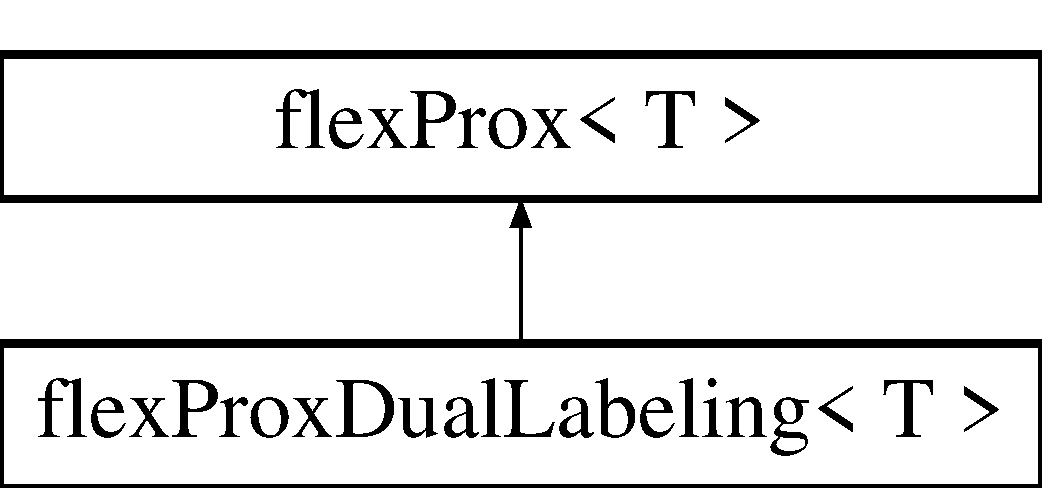
\includegraphics[height=2.000000cm]{classflex_prox_dual_labeling}
\end{center}
\end{figure}
\subsection*{Public Member Functions}
\begin{DoxyCompactItemize}
\item 
void \hyperlink{classflex_prox_dual_labeling_a29e89f413ea586b9390da273141c823b}{apply\+Prox} (T alpha, \hyperlink{classflex_box_data}{flex\+Box\+Data}$<$ T $>$ $\ast$data, const std\+::vector$<$ int $>$ \&dual\+Numbers, const std\+::vector$<$ int $>$ \&primal\+Numbers)
\begin{DoxyCompactList}\small\item\em applies prox for non-\/data terms \end{DoxyCompactList}\item 
void \hyperlink{classflex_prox_dual_labeling_a224460146ef61af8b939e4a961cbe776}{apply\+Prox} (T alpha, \hyperlink{classflex_box_data}{flex\+Box\+Data}$<$ T $>$ $\ast$data, const std\+::vector$<$ int $>$ \&dual\+Numbers, const std\+::vector$<$ int $>$ \&primal\+Numbers, std\+::vector$<$ Tdata $>$ \&f\+List)
\begin{DoxyCompactList}\small\item\em applies prox for data terms \end{DoxyCompactList}\end{DoxyCompactItemize}
\subsection*{Additional Inherited Members}


\subsection{Detailed Description}
\subsubsection*{template$<$typename T$>$\newline
class flex\+Prox\+Dual\+Labeling$<$ T $>$}

represents prox for a labeling term 

$ \sum_i \langle u_i,f_i\rangle + \delta_{ \{\bar{u}_1,\ldots,\bar{u}_n : \bar{u}_i \geq 0, \sum_i u_i = 1 \}}(u_1,\ldots,u_n) $ 

\subsection{Member Function Documentation}
\mbox{\Hypertarget{classflex_prox_dual_labeling_a29e89f413ea586b9390da273141c823b}\label{classflex_prox_dual_labeling_a29e89f413ea586b9390da273141c823b}} 
\index{flex\+Prox\+Dual\+Labeling@{flex\+Prox\+Dual\+Labeling}!apply\+Prox@{apply\+Prox}}
\index{apply\+Prox@{apply\+Prox}!flex\+Prox\+Dual\+Labeling@{flex\+Prox\+Dual\+Labeling}}
\subsubsection{\texorpdfstring{apply\+Prox()}{applyProx()}\hspace{0.1cm}{\footnotesize\ttfamily [1/2]}}
{\footnotesize\ttfamily template$<$typename T $>$ \\
void \hyperlink{classflex_prox_dual_labeling}{flex\+Prox\+Dual\+Labeling}$<$ T $>$\+::apply\+Prox (\begin{DoxyParamCaption}\item[{T}]{alpha,  }\item[{\hyperlink{classflex_box_data}{flex\+Box\+Data}$<$ T $>$ $\ast$}]{data,  }\item[{const std\+::vector$<$ int $>$ \&}]{dual\+Numbers,  }\item[{const std\+::vector$<$ int $>$ \&}]{primal\+Numbers }\end{DoxyParamCaption})\hspace{0.3cm}{\ttfamily [inline]}, {\ttfamily [virtual]}}



applies prox for non-\/data terms 

the function body should be empty if implemented prox is a data prox 
\begin{DoxyParams}{Parameters}
{\em alpha} & weight of term \\
\hline
{\em data} & data object \\
\hline
{\em dual\+Numbers} & vector of internal identifactions of dual numbers corresponding to the term \\
\hline
\end{DoxyParams}
\begin{DoxySeeAlso}{See also}
\hyperlink{classflex_box}{flex\+Box} 
\end{DoxySeeAlso}

\begin{DoxyParams}{Parameters}
{\em primal\+Numbers} & vector of internal identifactions of primal numbers corresponding to the term \\
\hline
\end{DoxyParams}
\begin{DoxySeeAlso}{See also}
\hyperlink{classflex_box}{flex\+Box} 
\end{DoxySeeAlso}


Implements \hyperlink{classflex_prox_a6d3119bd368c4216ad264a1f6dc1d01f}{flex\+Prox$<$ T $>$}.

\mbox{\Hypertarget{classflex_prox_dual_labeling_a224460146ef61af8b939e4a961cbe776}\label{classflex_prox_dual_labeling_a224460146ef61af8b939e4a961cbe776}} 
\index{flex\+Prox\+Dual\+Labeling@{flex\+Prox\+Dual\+Labeling}!apply\+Prox@{apply\+Prox}}
\index{apply\+Prox@{apply\+Prox}!flex\+Prox\+Dual\+Labeling@{flex\+Prox\+Dual\+Labeling}}
\subsubsection{\texorpdfstring{apply\+Prox()}{applyProx()}\hspace{0.1cm}{\footnotesize\ttfamily [2/2]}}
{\footnotesize\ttfamily template$<$typename T $>$ \\
void \hyperlink{classflex_prox_dual_labeling}{flex\+Prox\+Dual\+Labeling}$<$ T $>$\+::apply\+Prox (\begin{DoxyParamCaption}\item[{T}]{alpha,  }\item[{\hyperlink{classflex_box_data}{flex\+Box\+Data}$<$ T $>$ $\ast$}]{data,  }\item[{const std\+::vector$<$ int $>$ \&}]{dual\+Numbers,  }\item[{const std\+::vector$<$ int $>$ \&}]{primal\+Numbers,  }\item[{std\+::vector$<$ Tdata $>$ \&}]{f\+List }\end{DoxyParamCaption})\hspace{0.3cm}{\ttfamily [inline]}, {\ttfamily [virtual]}}



applies prox for data terms 

the function body should be empty if implemented prox is a non-\/data prox 
\begin{DoxyParams}{Parameters}
{\em alpha} & weight of term \\
\hline
{\em data} & data object \\
\hline
{\em dual\+Numbers} & vector of internal identifactions of dual numbers corresponding to the term \\
\hline
\end{DoxyParams}
\begin{DoxySeeAlso}{See also}
\hyperlink{classflex_box}{flex\+Box} 
\end{DoxySeeAlso}

\begin{DoxyParams}{Parameters}
{\em primal\+Numbers} & vector of internal identifactions of primal numbers corresponding to the term \\
\hline
\end{DoxyParams}
\begin{DoxySeeAlso}{See also}
\hyperlink{classflex_box}{flex\+Box} 
\end{DoxySeeAlso}

\begin{DoxyParams}{Parameters}
{\em f\+List} & data part of term \\
\hline
\end{DoxyParams}


Implements \hyperlink{classflex_prox_aec433ffbf1a7586f26a2116c6b94bdd6}{flex\+Prox$<$ T $>$}.



The documentation for this class was generated from the following file\+:\begin{DoxyCompactItemize}
\item 
flex\+Prox\+Dual\+Labeling.\+h\end{DoxyCompactItemize}

\hypertarget{classflex_prox_dual_l_inf}{}\section{flex\+Prox\+Dual\+L\+Inf$<$ T $>$ Class Template Reference}
\label{classflex_prox_dual_l_inf}\index{flex\+Prox\+Dual\+L\+Inf$<$ T $>$@{flex\+Prox\+Dual\+L\+Inf$<$ T $>$}}


represents prox for a L\+Inf non-\/data term  




{\ttfamily \#include $<$flex\+Prox\+Dual\+L\+Inf.\+h$>$}

Inheritance diagram for flex\+Prox\+Dual\+L\+Inf$<$ T $>$\+:\begin{figure}[H]
\begin{center}
\leavevmode
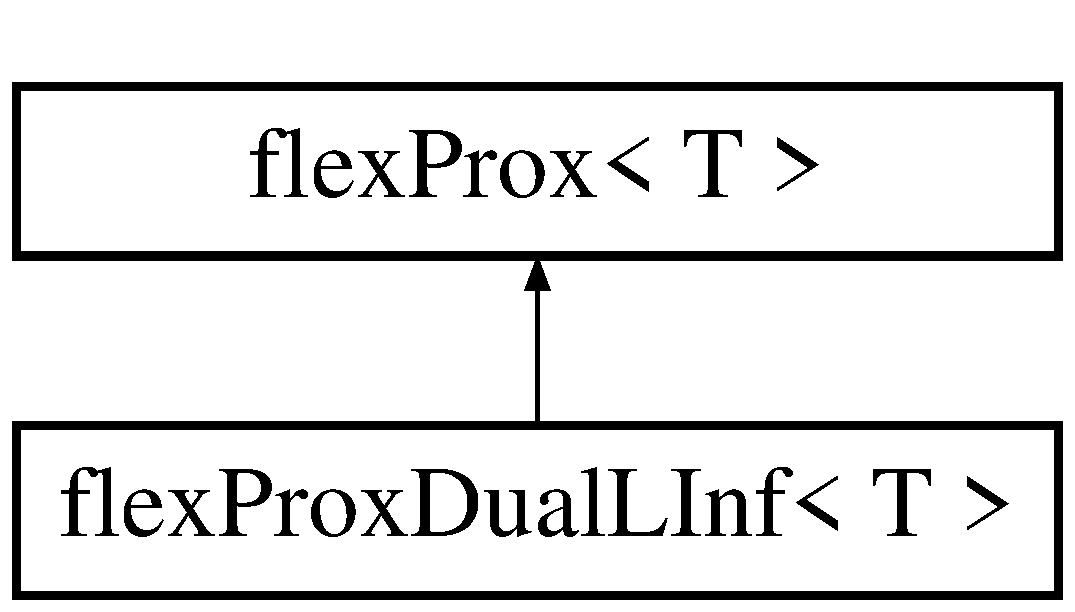
\includegraphics[height=2.000000cm]{classflex_prox_dual_l_inf}
\end{center}
\end{figure}
\subsection*{Classes}
\begin{DoxyCompactItemize}
\item 
struct {\bfseries Abs\+Functor}
\item 
struct {\bfseries Compare\+Functor}
\item 
struct {\bfseries Find\+Functor}
\item 
struct {\bfseries Update\+Y\+Functor}
\end{DoxyCompactItemize}
\subsection*{Public Member Functions}
\begin{DoxyCompactItemize}
\item 
void \hyperlink{classflex_prox_dual_l_inf_a90e3ad5244d8bf6cef50541593fb9da0}{apply\+Prox} (T alpha, \hyperlink{classflex_box_data}{flex\+Box\+Data}$<$ T $>$ $\ast$data, const std\+::vector$<$ int $>$ \&dual\+Numbers, const std\+::vector$<$ int $>$ \&primal\+Numbers)
\begin{DoxyCompactList}\small\item\em applies prox for non-\/data terms \end{DoxyCompactList}\item 
void \hyperlink{classflex_prox_dual_l_inf_a3ead6ede3f9535c5540c91955f83313b}{apply\+Prox} (T alpha, \hyperlink{classflex_box_data}{flex\+Box\+Data}$<$ T $>$ $\ast$data, const std\+::vector$<$ int $>$ \&dual\+Numbers, const std\+::vector$<$ int $>$ \&primal\+Numbers, std\+::vector$<$ Tdata $>$ \&f\+List)
\begin{DoxyCompactList}\small\item\em applies prox for data terms \end{DoxyCompactList}\end{DoxyCompactItemize}
\subsection*{Additional Inherited Members}


\subsection{Detailed Description}
\subsubsection*{template$<$typename T$>$\newline
class flex\+Prox\+Dual\+L\+Inf$<$ T $>$}

represents prox for a L\+Inf non-\/data term 

$ \alpha \|\cdot\|_{\infty} $ 

\subsection{Member Function Documentation}
\mbox{\Hypertarget{classflex_prox_dual_l_inf_a90e3ad5244d8bf6cef50541593fb9da0}\label{classflex_prox_dual_l_inf_a90e3ad5244d8bf6cef50541593fb9da0}} 
\index{flex\+Prox\+Dual\+L\+Inf@{flex\+Prox\+Dual\+L\+Inf}!apply\+Prox@{apply\+Prox}}
\index{apply\+Prox@{apply\+Prox}!flex\+Prox\+Dual\+L\+Inf@{flex\+Prox\+Dual\+L\+Inf}}
\subsubsection{\texorpdfstring{apply\+Prox()}{applyProx()}\hspace{0.1cm}{\footnotesize\ttfamily [1/2]}}
{\footnotesize\ttfamily template$<$typename T $>$ \\
void \hyperlink{classflex_prox_dual_l_inf}{flex\+Prox\+Dual\+L\+Inf}$<$ T $>$\+::apply\+Prox (\begin{DoxyParamCaption}\item[{T}]{alpha,  }\item[{\hyperlink{classflex_box_data}{flex\+Box\+Data}$<$ T $>$ $\ast$}]{data,  }\item[{const std\+::vector$<$ int $>$ \&}]{dual\+Numbers,  }\item[{const std\+::vector$<$ int $>$ \&}]{primal\+Numbers }\end{DoxyParamCaption})\hspace{0.3cm}{\ttfamily [inline]}, {\ttfamily [virtual]}}



applies prox for non-\/data terms 

the function body should be empty if implemented prox is a data prox 
\begin{DoxyParams}{Parameters}
{\em alpha} & weight of term \\
\hline
{\em data} & data object \\
\hline
{\em dual\+Numbers} & vector of internal identifactions of dual numbers corresponding to the term \\
\hline
\end{DoxyParams}
\begin{DoxySeeAlso}{See also}
\hyperlink{classflex_box}{flex\+Box} 
\end{DoxySeeAlso}

\begin{DoxyParams}{Parameters}
{\em primal\+Numbers} & vector of internal identifactions of primal numbers corresponding to the term \\
\hline
\end{DoxyParams}
\begin{DoxySeeAlso}{See also}
\hyperlink{classflex_box}{flex\+Box} 
\end{DoxySeeAlso}


Implements \hyperlink{classflex_prox_a6d3119bd368c4216ad264a1f6dc1d01f}{flex\+Prox$<$ T $>$}.

\mbox{\Hypertarget{classflex_prox_dual_l_inf_a3ead6ede3f9535c5540c91955f83313b}\label{classflex_prox_dual_l_inf_a3ead6ede3f9535c5540c91955f83313b}} 
\index{flex\+Prox\+Dual\+L\+Inf@{flex\+Prox\+Dual\+L\+Inf}!apply\+Prox@{apply\+Prox}}
\index{apply\+Prox@{apply\+Prox}!flex\+Prox\+Dual\+L\+Inf@{flex\+Prox\+Dual\+L\+Inf}}
\subsubsection{\texorpdfstring{apply\+Prox()}{applyProx()}\hspace{0.1cm}{\footnotesize\ttfamily [2/2]}}
{\footnotesize\ttfamily template$<$typename T $>$ \\
void \hyperlink{classflex_prox_dual_l_inf}{flex\+Prox\+Dual\+L\+Inf}$<$ T $>$\+::apply\+Prox (\begin{DoxyParamCaption}\item[{T}]{alpha,  }\item[{\hyperlink{classflex_box_data}{flex\+Box\+Data}$<$ T $>$ $\ast$}]{data,  }\item[{const std\+::vector$<$ int $>$ \&}]{dual\+Numbers,  }\item[{const std\+::vector$<$ int $>$ \&}]{primal\+Numbers,  }\item[{std\+::vector$<$ Tdata $>$ \&}]{f\+List }\end{DoxyParamCaption})\hspace{0.3cm}{\ttfamily [inline]}, {\ttfamily [virtual]}}



applies prox for data terms 

the function body should be empty if implemented prox is a non-\/data prox 
\begin{DoxyParams}{Parameters}
{\em alpha} & weight of term \\
\hline
{\em data} & data object \\
\hline
{\em dual\+Numbers} & vector of internal identifactions of dual numbers corresponding to the term \\
\hline
\end{DoxyParams}
\begin{DoxySeeAlso}{See also}
\hyperlink{classflex_box}{flex\+Box} 
\end{DoxySeeAlso}

\begin{DoxyParams}{Parameters}
{\em primal\+Numbers} & vector of internal identifactions of primal numbers corresponding to the term \\
\hline
\end{DoxyParams}
\begin{DoxySeeAlso}{See also}
\hyperlink{classflex_box}{flex\+Box} 
\end{DoxySeeAlso}

\begin{DoxyParams}{Parameters}
{\em f\+List} & data part of term \\
\hline
\end{DoxyParams}


Implements \hyperlink{classflex_prox_aec433ffbf1a7586f26a2116c6b94bdd6}{flex\+Prox$<$ T $>$}.



The documentation for this class was generated from the following file\+:\begin{DoxyCompactItemize}
\item 
flex\+Prox\+Dual\+L\+Inf.\+h\end{DoxyCompactItemize}

\hypertarget{classflex_solver}{}\section{flex\+Solver$<$ T $>$ Class Template Reference}
\label{classflex_solver}\index{flex\+Solver$<$ T $>$@{flex\+Solver$<$ T $>$}}


Flex\+Box solver class.  




{\ttfamily \#include $<$flex\+Solver.\+h$>$}

Inheritance diagram for flex\+Solver$<$ T $>$\+:\begin{figure}[H]
\begin{center}
\leavevmode
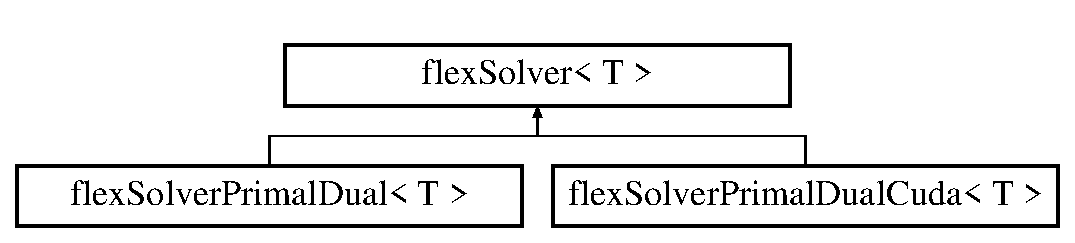
\includegraphics[height=2.000000cm]{classflex_solver}
\end{center}
\end{figure}
\subsection*{Public Member Functions}
\begin{DoxyCompactItemize}
\item 
\mbox{\Hypertarget{classflex_solver_a072d7af0f075d53b2efb6a119fbc6280}\label{classflex_solver_a072d7af0f075d53b2efb6a119fbc6280}} 
virtual void {\bfseries init} (\hyperlink{classflex_box_data}{flex\+Box\+Data}$<$ T $>$ $\ast$data)=0
\item 
\mbox{\Hypertarget{classflex_solver_ad496971c4d875162b0ce7c675232956e}\label{classflex_solver_ad496971c4d875162b0ce7c675232956e}} 
virtual void {\bfseries add\+Term} (\hyperlink{classflex_box_data}{flex\+Box\+Data}$<$ T $>$ $\ast$data, \hyperlink{classflex_term}{flex\+Term}$<$ T $>$ $\ast$\+\_\+dual\+Part, std\+::vector$<$ int $>$ \+\_\+corresponding\+Primals)=0
\item 
\mbox{\Hypertarget{classflex_solver_a61ba0cf7b87a326c5360b334b5e48f25}\label{classflex_solver_a61ba0cf7b87a326c5360b334b5e48f25}} 
virtual void {\bfseries do\+Iteration} (\hyperlink{classflex_box_data}{flex\+Box\+Data}$<$ T $>$ $\ast$data)=0
\item 
\mbox{\Hypertarget{classflex_solver_a0ba40198cc0c2f46c81c1981a505f7e9}\label{classflex_solver_a0ba40198cc0c2f46c81c1981a505f7e9}} 
virtual T {\bfseries calculate\+Error} (\hyperlink{classflex_box_data}{flex\+Box\+Data}$<$ T $>$ $\ast$data)=0
\end{DoxyCompactItemize}


\subsection{Detailed Description}
\subsubsection*{template$<$typename T$>$\newline
class flex\+Solver$<$ T $>$}

Flex\+Box solver class. 

\hyperlink{classflex_solver}{flex\+Solver} is an internal abstract class for running the primal dual algortihm used by the \hyperlink{classflex_box}{flex\+Box} main class. This class should not be used directly. 

The documentation for this class was generated from the following file\+:\begin{DoxyCompactItemize}
\item 
flex\+Solver.\+h\end{DoxyCompactItemize}

\hypertarget{classflex_solver_primal_dual}{}\section{flex\+Solver\+Primal\+Dual$<$ T $>$ Class Template Reference}
\label{classflex_solver_primal_dual}\index{flex\+Solver\+Primal\+Dual$<$ T $>$@{flex\+Solver\+Primal\+Dual$<$ T $>$}}


Flex\+Box solver class if using the non-\/\+C\+U\+DA version.  




{\ttfamily \#include $<$flex\+Solver\+Primal\+Dual.\+h$>$}

Inheritance diagram for flex\+Solver\+Primal\+Dual$<$ T $>$\+:\begin{figure}[H]
\begin{center}
\leavevmode
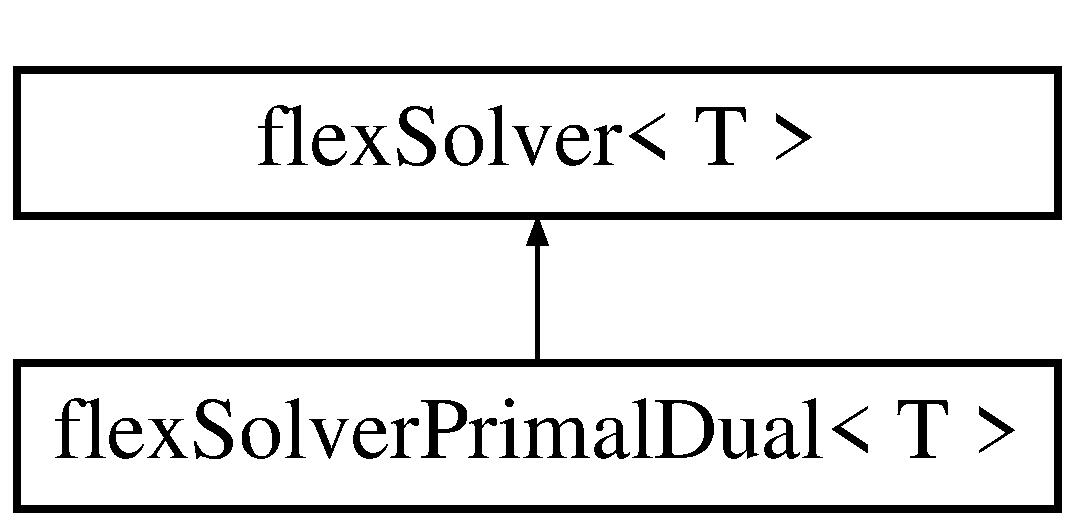
\includegraphics[height=2.000000cm]{classflex_solver_primal_dual}
\end{center}
\end{figure}
\subsection*{Public Member Functions}
\begin{DoxyCompactItemize}
\item 
\mbox{\Hypertarget{classflex_solver_primal_dual_a336d1da6eead54255c6f775f945246ba}\label{classflex_solver_primal_dual_a336d1da6eead54255c6f775f945246ba}} 
void {\bfseries init} (\hyperlink{classflex_box_data}{flex\+Box\+Data}$<$ T $>$ $\ast$data)
\item 
\mbox{\Hypertarget{classflex_solver_primal_dual_a3247dd2a9af9b3acaccf93099ea6cad7}\label{classflex_solver_primal_dual_a3247dd2a9af9b3acaccf93099ea6cad7}} 
void {\bfseries calculate\+Tau\+Sigma} (\hyperlink{classflex_box_data}{flex\+Box\+Data}$<$ T $>$ $\ast$data)
\item 
\mbox{\Hypertarget{classflex_solver_primal_dual_aef2b795a7019f88dbfc335725ac9ae91}\label{classflex_solver_primal_dual_aef2b795a7019f88dbfc335725ac9ae91}} 
void {\bfseries add\+Term} (\hyperlink{classflex_box_data}{flex\+Box\+Data}$<$ T $>$ $\ast$data, \hyperlink{classflex_term}{flex\+Term}$<$ T $>$ $\ast$a\+Dual\+Part, std\+::vector$<$ int $>$ a\+Corresponding\+Primals)
\item 
\mbox{\Hypertarget{classflex_solver_primal_dual_a22ace8e6df1ab56e16bb196965f894e8}\label{classflex_solver_primal_dual_a22ace8e6df1ab56e16bb196965f894e8}} 
void {\bfseries y\+Tilde} (\hyperlink{classflex_box_data}{flex\+Box\+Data}$<$ T $>$ $\ast$data, \hyperlink{classflex_term}{flex\+Term}$<$ T $>$ $\ast$dual\+Term, const std\+::vector$<$ int $>$ \&dual\+Numbers, const std\+::vector$<$ int $>$ \&primal\+Numbers)
\item 
\mbox{\Hypertarget{classflex_solver_primal_dual_a78d23897067a5941ee58b7f45433831e}\label{classflex_solver_primal_dual_a78d23897067a5941ee58b7f45433831e}} 
void {\bfseries x\+Tilde} (\hyperlink{classflex_box_data}{flex\+Box\+Data}$<$ T $>$ $\ast$data, \hyperlink{classflex_term}{flex\+Term}$<$ T $>$ $\ast$dual\+Term, const std\+::vector$<$ int $>$ \&dual\+Numbers, const std\+::vector$<$ int $>$ \&primal\+Numbers)
\item 
\mbox{\Hypertarget{classflex_solver_primal_dual_a6d072be7a02617f61011c50b13547d7a}\label{classflex_solver_primal_dual_a6d072be7a02617f61011c50b13547d7a}} 
void {\bfseries do\+Iteration} (\hyperlink{classflex_box_data}{flex\+Box\+Data}$<$ T $>$ $\ast$data)
\item 
\mbox{\Hypertarget{classflex_solver_primal_dual_a8358fe4f17725997a4fe178151ab7e8a}\label{classflex_solver_primal_dual_a8358fe4f17725997a4fe178151ab7e8a}} 
void {\bfseries y\+Error} (\hyperlink{classflex_box_data}{flex\+Box\+Data}$<$ T $>$ $\ast$data, \hyperlink{classflex_term}{flex\+Term}$<$ T $>$ $\ast$dual\+Term, const std\+::vector$<$ int $>$ \&dual\+Numbers, const std\+::vector$<$ int $>$ \&primal\+Numbers)
\item 
\mbox{\Hypertarget{classflex_solver_primal_dual_a533b774914fb5059ca132408bb4c6308}\label{classflex_solver_primal_dual_a533b774914fb5059ca132408bb4c6308}} 
void {\bfseries x\+Error} (\hyperlink{classflex_box_data}{flex\+Box\+Data}$<$ T $>$ $\ast$data, \hyperlink{classflex_term}{flex\+Term}$<$ T $>$ $\ast$dual\+Term, const std\+::vector$<$ int $>$ \&dual\+Numbers, const std\+::vector$<$ int $>$ \&primal\+Numbers)
\item 
\mbox{\Hypertarget{classflex_solver_primal_dual_a769d3d8fb150ad88e264fde8e5a5e1ab}\label{classflex_solver_primal_dual_a769d3d8fb150ad88e264fde8e5a5e1ab}} 
T {\bfseries calculate\+Error} (\hyperlink{classflex_box_data}{flex\+Box\+Data}$<$ T $>$ $\ast$data)
\end{DoxyCompactItemize}


\subsection{Detailed Description}
\subsubsection*{template$<$typename T$>$\newline
class flex\+Solver\+Primal\+Dual$<$ T $>$}

Flex\+Box solver class if using the non-\/\+C\+U\+DA version. 

\hyperlink{classflex_solver_primal_dual}{flex\+Solver\+Primal\+Dual} is an internal class for running the primal dual algortihm if using the non-\/\+C\+U\+DA version. This class should not be used directly. 

The documentation for this class was generated from the following file\+:\begin{DoxyCompactItemize}
\item 
flex\+Solver\+Primal\+Dual.\+h\end{DoxyCompactItemize}

\hypertarget{classflex_solver_primal_dual_cuda}{}\section{flex\+Solver\+Primal\+Dual\+Cuda$<$ T $>$ Class Template Reference}
\label{classflex_solver_primal_dual_cuda}\index{flex\+Solver\+Primal\+Dual\+Cuda$<$ T $>$@{flex\+Solver\+Primal\+Dual\+Cuda$<$ T $>$}}


Flex\+Box solver class if using the C\+U\+DA version.  




{\ttfamily \#include $<$flex\+Solver\+Primal\+Dual\+Cuda.\+h$>$}

Inheritance diagram for flex\+Solver\+Primal\+Dual\+Cuda$<$ T $>$\+:\begin{figure}[H]
\begin{center}
\leavevmode
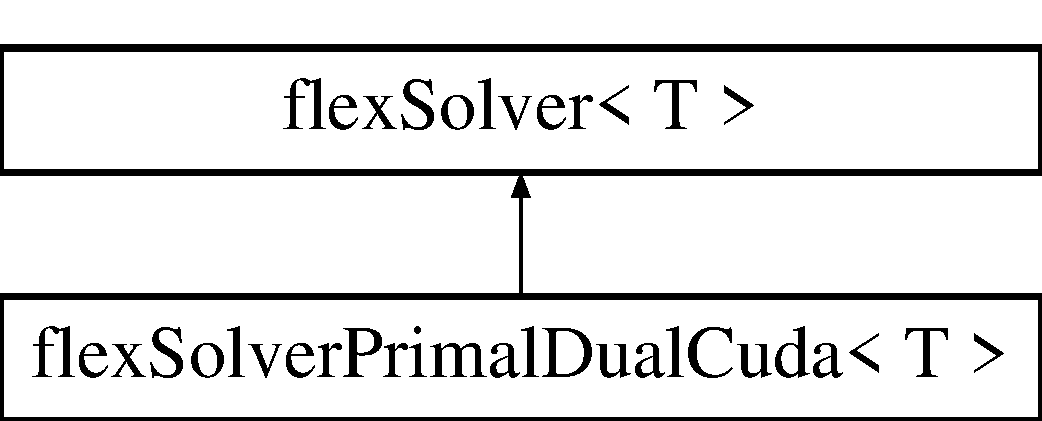
\includegraphics[height=2.000000cm]{classflex_solver_primal_dual_cuda}
\end{center}
\end{figure}
\subsection*{Classes}
\begin{DoxyCompactItemize}
\item 
struct {\bfseries calculate\+Error\+Functor}
\item 
struct {\bfseries x\+Tilde\+Functor}
\item 
struct {\bfseries y\+Tilde\+Functor}
\end{DoxyCompactItemize}
\subsection*{Public Member Functions}
\begin{DoxyCompactItemize}
\item 
\mbox{\Hypertarget{classflex_solver_primal_dual_cuda_a41d4d35abe71c6d2fdd79d460f6f8306}\label{classflex_solver_primal_dual_cuda_a41d4d35abe71c6d2fdd79d460f6f8306}} 
void {\bfseries init} (\hyperlink{classflex_box_data}{flex\+Box\+Data}$<$ T $>$ $\ast$data)
\item 
\mbox{\Hypertarget{classflex_solver_primal_dual_cuda_a80d051306bf6354cad9654181e5080b9}\label{classflex_solver_primal_dual_cuda_a80d051306bf6354cad9654181e5080b9}} 
void {\bfseries calculate\+Tau\+Sigma} (\hyperlink{classflex_box_data}{flex\+Box\+Data}$<$ T $>$ $\ast$data)
\item 
\mbox{\Hypertarget{classflex_solver_primal_dual_cuda_aa7e9fe5b975a1a5e3a74440da7a0245a}\label{classflex_solver_primal_dual_cuda_aa7e9fe5b975a1a5e3a74440da7a0245a}} 
void {\bfseries add\+Term} (\hyperlink{classflex_box_data}{flex\+Box\+Data}$<$ T $>$ $\ast$data, \hyperlink{classflex_term}{flex\+Term}$<$ T $>$ $\ast$\+\_\+dual\+Part, std\+::vector$<$ int $>$ \+\_\+corresponding\+Primals)
\item 
\mbox{\Hypertarget{classflex_solver_primal_dual_cuda_a0e866f64654ee21f7105a3e38447621c}\label{classflex_solver_primal_dual_cuda_a0e866f64654ee21f7105a3e38447621c}} 
void {\bfseries y\+Tilde} (\hyperlink{classflex_box_data}{flex\+Box\+Data}$<$ T $>$ $\ast$data, \hyperlink{classflex_term}{flex\+Term}$<$ T $>$ $\ast$dual\+Term, const std\+::vector$<$ int $>$ \&dual\+Numbers, const std\+::vector$<$ int $>$ \&primal\+Numbers)
\item 
\mbox{\Hypertarget{classflex_solver_primal_dual_cuda_ad254501e2e09f300df111c502b4f40aa}\label{classflex_solver_primal_dual_cuda_ad254501e2e09f300df111c502b4f40aa}} 
void {\bfseries x\+Tilde} (\hyperlink{classflex_box_data}{flex\+Box\+Data}$<$ T $>$ $\ast$data, \hyperlink{classflex_term}{flex\+Term}$<$ T $>$ $\ast$dual\+Term, const std\+::vector$<$ int $>$ \&dual\+Numbers, const std\+::vector$<$ int $>$ \&primal\+Numbers)
\item 
\mbox{\Hypertarget{classflex_solver_primal_dual_cuda_a4790bcbc1a7711002ffb9c6c6b29c05f}\label{classflex_solver_primal_dual_cuda_a4790bcbc1a7711002ffb9c6c6b29c05f}} 
void {\bfseries do\+Iteration} (\hyperlink{classflex_box_data}{flex\+Box\+Data}$<$ T $>$ $\ast$data)
\item 
\mbox{\Hypertarget{classflex_solver_primal_dual_cuda_a983fcb3ec45e57491a6be6179ba23a90}\label{classflex_solver_primal_dual_cuda_a983fcb3ec45e57491a6be6179ba23a90}} 
void {\bfseries y\+Error} (\hyperlink{classflex_box_data}{flex\+Box\+Data}$<$ T $>$ $\ast$data, \hyperlink{classflex_term}{flex\+Term}$<$ T $>$ $\ast$dual\+Term, const std\+::vector$<$ int $>$ \&dual\+Numbers, const std\+::vector$<$ int $>$ \&primal\+Numbers)
\item 
\mbox{\Hypertarget{classflex_solver_primal_dual_cuda_a52e5086520e5590b1d26deabb989b39b}\label{classflex_solver_primal_dual_cuda_a52e5086520e5590b1d26deabb989b39b}} 
void {\bfseries x\+Error} (\hyperlink{classflex_box_data}{flex\+Box\+Data}$<$ T $>$ $\ast$data, \hyperlink{classflex_term}{flex\+Term}$<$ T $>$ $\ast$dual\+Term, const std\+::vector$<$ int $>$ \&dual\+Numbers, const std\+::vector$<$ int $>$ \&primal\+Numbers)
\item 
\mbox{\Hypertarget{classflex_solver_primal_dual_cuda_a8d08313435dad5b2fd832570fdf42263}\label{classflex_solver_primal_dual_cuda_a8d08313435dad5b2fd832570fdf42263}} 
T {\bfseries calculate\+Error} (\hyperlink{classflex_box_data}{flex\+Box\+Data}$<$ T $>$ $\ast$data)
\end{DoxyCompactItemize}


\subsection{Detailed Description}
\subsubsection*{template$<$typename T$>$\newline
class flex\+Solver\+Primal\+Dual\+Cuda$<$ T $>$}

Flex\+Box solver class if using the C\+U\+DA version. 

\hyperlink{classflex_solver_primal_dual}{flex\+Solver\+Primal\+Dual} is an internal class for running the primal dual algortihm if using the C\+U\+DA version. This class should not be used directly. 

The documentation for this class was generated from the following file\+:\begin{DoxyCompactItemize}
\item 
flex\+Solver\+Primal\+Dual\+Cuda.\+h\end{DoxyCompactItemize}

\hypertarget{classflex_superpixel_operator}{}\section{flex\+Superpixel\+Operator$<$ T $>$ Class Template Reference}
\label{classflex_superpixel_operator}\index{flex\+Superpixel\+Operator$<$ T $>$@{flex\+Superpixel\+Operator$<$ T $>$}}


represents a superpixel operator  




{\ttfamily \#include $<$flex\+Superpixel\+Operator.\+h$>$}

Inheritance diagram for flex\+Superpixel\+Operator$<$ T $>$\+:\begin{figure}[H]
\begin{center}
\leavevmode
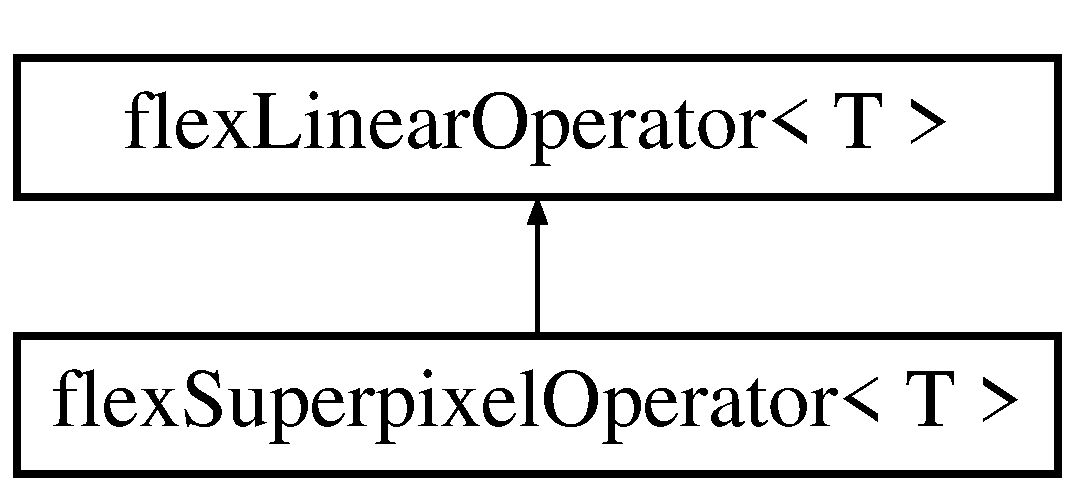
\includegraphics[height=2.000000cm]{classflex_superpixel_operator}
\end{center}
\end{figure}
\subsection*{Public Member Functions}
\begin{DoxyCompactItemize}
\item 
\hyperlink{classflex_superpixel_operator_a810ff259aed4c17eed5b6c731bb59b3b}{flex\+Superpixel\+Operator} (std\+::vector$<$ int $>$ a\+Target\+Dimension, T a\+Upsampling\+Factor, bool a\+Minus)
\begin{DoxyCompactList}\small\item\em initializes the superpixel operator. Downsamples image of size a\+Upsampling\+Factor $\ast$ a\+Target\+Dimension to size a\+Target\+Dimension \end{DoxyCompactList}\item 
\hyperlink{classflex_superpixel_operator}{flex\+Superpixel\+Operator}$<$ T $>$ $\ast$ \hyperlink{classflex_superpixel_operator_ab0e066735127a3b39958c6719fe03156}{copy} ()
\begin{DoxyCompactList}\small\item\em copies the linear operator \end{DoxyCompactList}\item 
void \hyperlink{classflex_superpixel_operator_afa075c0858c693342646250225f7c425}{times} (bool transposed, const Tdata \&input, Tdata \&output)
\begin{DoxyCompactList}\small\item\em applies linear operator on vector \end{DoxyCompactList}\item 
void \hyperlink{classflex_superpixel_operator_aa9c40f1e42786b6fe9cd698cf15028fc}{times\+Plus} (bool transposed, const Tdata \&input, Tdata \&output)
\begin{DoxyCompactList}\small\item\em applies linear operator on vector and adds its result to y \end{DoxyCompactList}\item 
void \hyperlink{classflex_superpixel_operator_af0831ae77a7e8c894a110146a316c944}{times\+Minus} (bool transposed, const Tdata \&input, Tdata \&output)
\begin{DoxyCompactList}\small\item\em applies linear operator on vector and substracts its result from y \end{DoxyCompactList}\item 
std\+::vector$<$ T $>$ \hyperlink{classflex_superpixel_operator_afd3f55401eaa6fb3e8a62c7f83443a4d}{get\+Abs\+Row\+Sum} (bool transposed)
\begin{DoxyCompactList}\small\item\em returns a vector of sum of absolute values per row used for preconditioning \end{DoxyCompactList}\item 
T \hyperlink{classflex_superpixel_operator_a83c4978b05be05c45be7d2ea58e96b44}{get\+Max\+Row\+Sum\+Abs} (bool transposed)
\begin{DoxyCompactList}\small\item\em returns the maximum sum of absolute values per row used for preconditioning \end{DoxyCompactList}\item 
thrust\+::device\+\_\+vector$<$ T $>$ \hyperlink{classflex_superpixel_operator_ae2f878d68c4574a0d5f21ffd132afc63}{get\+Abs\+Row\+Sum\+C\+U\+DA} (bool transposed)
\begin{DoxyCompactList}\small\item\em same function as \hyperlink{classflex_superpixel_operator_afd3f55401eaa6fb3e8a62c7f83443a4d}{get\+Abs\+Row\+Sum()} but implemented in C\+U\+DA \end{DoxyCompactList}\end{DoxyCompactItemize}
\subsection*{Additional Inherited Members}


\subsection{Detailed Description}
\subsubsection*{template$<$typename T$>$\newline
class flex\+Superpixel\+Operator$<$ T $>$}

represents a superpixel operator 

downsamples data of size upsampling\+Factor $\ast$ target\+Dimension size to target\+Dimension 

\subsection{Constructor \& Destructor Documentation}
\mbox{\Hypertarget{classflex_superpixel_operator_a810ff259aed4c17eed5b6c731bb59b3b}\label{classflex_superpixel_operator_a810ff259aed4c17eed5b6c731bb59b3b}} 
\index{flex\+Superpixel\+Operator@{flex\+Superpixel\+Operator}!flex\+Superpixel\+Operator@{flex\+Superpixel\+Operator}}
\index{flex\+Superpixel\+Operator@{flex\+Superpixel\+Operator}!flex\+Superpixel\+Operator@{flex\+Superpixel\+Operator}}
\subsubsection{\texorpdfstring{flex\+Superpixel\+Operator()}{flexSuperpixelOperator()}}
{\footnotesize\ttfamily template$<$typename T$>$ \\
\hyperlink{classflex_superpixel_operator}{flex\+Superpixel\+Operator}$<$ T $>$\+::\hyperlink{classflex_superpixel_operator}{flex\+Superpixel\+Operator} (\begin{DoxyParamCaption}\item[{std\+::vector$<$ int $>$}]{a\+Target\+Dimension,  }\item[{T}]{a\+Upsampling\+Factor,  }\item[{bool}]{a\+Minus }\end{DoxyParamCaption})\hspace{0.3cm}{\ttfamily [inline]}}



initializes the superpixel operator. Downsamples image of size a\+Upsampling\+Factor $\ast$ a\+Target\+Dimension to size a\+Target\+Dimension 


\begin{DoxyParams}{Parameters}
{\em a\+Target\+Dimension} & target dimension of downsampled image \\
\hline
{\em a\+Upsampling\+Factor} & a\+Upsampling\+Factor $\ast$ a\+Target\+Dimension is original image size \\
\hline
{\em a\+Minus} & determines if operator is negated \\
\hline
\end{DoxyParams}
\begin{DoxySeeAlso}{See also}
\hyperlink{classflex_linear_operator_a7f986517e10aee21099ec7692b77905d}{is\+Minus} 
\end{DoxySeeAlso}


\subsection{Member Function Documentation}
\mbox{\Hypertarget{classflex_superpixel_operator_ab0e066735127a3b39958c6719fe03156}\label{classflex_superpixel_operator_ab0e066735127a3b39958c6719fe03156}} 
\index{flex\+Superpixel\+Operator@{flex\+Superpixel\+Operator}!copy@{copy}}
\index{copy@{copy}!flex\+Superpixel\+Operator@{flex\+Superpixel\+Operator}}
\subsubsection{\texorpdfstring{copy()}{copy()}}
{\footnotesize\ttfamily template$<$typename T$>$ \\
\hyperlink{classflex_superpixel_operator}{flex\+Superpixel\+Operator}$<$T$>$$\ast$ \hyperlink{classflex_superpixel_operator}{flex\+Superpixel\+Operator}$<$ T $>$\+::copy (\begin{DoxyParamCaption}{ }\end{DoxyParamCaption})\hspace{0.3cm}{\ttfamily [inline]}, {\ttfamily [virtual]}}



copies the linear operator 

\begin{DoxyReturn}{Returns}
copy of linear operator 
\end{DoxyReturn}


Implements \hyperlink{classflex_linear_operator_a7cc1425677cc30fcbd092ffd28d508c9}{flex\+Linear\+Operator$<$ T $>$}.

\mbox{\Hypertarget{classflex_superpixel_operator_afd3f55401eaa6fb3e8a62c7f83443a4d}\label{classflex_superpixel_operator_afd3f55401eaa6fb3e8a62c7f83443a4d}} 
\index{flex\+Superpixel\+Operator@{flex\+Superpixel\+Operator}!get\+Abs\+Row\+Sum@{get\+Abs\+Row\+Sum}}
\index{get\+Abs\+Row\+Sum@{get\+Abs\+Row\+Sum}!flex\+Superpixel\+Operator@{flex\+Superpixel\+Operator}}
\subsubsection{\texorpdfstring{get\+Abs\+Row\+Sum()}{getAbsRowSum()}}
{\footnotesize\ttfamily template$<$typename T$>$ \\
std\+::vector$<$T$>$ \hyperlink{classflex_superpixel_operator}{flex\+Superpixel\+Operator}$<$ T $>$\+::get\+Abs\+Row\+Sum (\begin{DoxyParamCaption}\item[{bool}]{transposed }\end{DoxyParamCaption})\hspace{0.3cm}{\ttfamily [inline]}, {\ttfamily [virtual]}}



returns a vector of sum of absolute values per row used for preconditioning 


\begin{DoxyParams}{Parameters}
{\em transposed} & is true if operator should be (temporarily) transposed before usage \\
\hline
\end{DoxyParams}
\begin{DoxyReturn}{Returns}
vector of sum of absolute values per row 
\end{DoxyReturn}


Implements \hyperlink{classflex_linear_operator_ad6caa7b09e6e3c401cadef61b8e2307e}{flex\+Linear\+Operator$<$ T $>$}.

\mbox{\Hypertarget{classflex_superpixel_operator_ae2f878d68c4574a0d5f21ffd132afc63}\label{classflex_superpixel_operator_ae2f878d68c4574a0d5f21ffd132afc63}} 
\index{flex\+Superpixel\+Operator@{flex\+Superpixel\+Operator}!get\+Abs\+Row\+Sum\+C\+U\+DA@{get\+Abs\+Row\+Sum\+C\+U\+DA}}
\index{get\+Abs\+Row\+Sum\+C\+U\+DA@{get\+Abs\+Row\+Sum\+C\+U\+DA}!flex\+Superpixel\+Operator@{flex\+Superpixel\+Operator}}
\subsubsection{\texorpdfstring{get\+Abs\+Row\+Sum\+C\+U\+D\+A()}{getAbsRowSumCUDA()}}
{\footnotesize\ttfamily template$<$typename T$>$ \\
thrust\+::device\+\_\+vector$<$T$>$ \hyperlink{classflex_superpixel_operator}{flex\+Superpixel\+Operator}$<$ T $>$\+::get\+Abs\+Row\+Sum\+C\+U\+DA (\begin{DoxyParamCaption}\item[{bool}]{transposed }\end{DoxyParamCaption})\hspace{0.3cm}{\ttfamily [inline]}, {\ttfamily [virtual]}}



same function as \hyperlink{classflex_superpixel_operator_afd3f55401eaa6fb3e8a62c7f83443a4d}{get\+Abs\+Row\+Sum()} but implemented in C\+U\+DA 


\begin{DoxyParams}{Parameters}
{\em transposed} & is true if operator should be (temporarily) transposed before usage \\
\hline
\end{DoxyParams}
\begin{DoxyReturn}{Returns}
vector of sum of absolute values per row 
\end{DoxyReturn}


Implements \hyperlink{classflex_linear_operator_a0a0a431d43f4f9d36cbee0d31ba5a29b}{flex\+Linear\+Operator$<$ T $>$}.

\mbox{\Hypertarget{classflex_superpixel_operator_a83c4978b05be05c45be7d2ea58e96b44}\label{classflex_superpixel_operator_a83c4978b05be05c45be7d2ea58e96b44}} 
\index{flex\+Superpixel\+Operator@{flex\+Superpixel\+Operator}!get\+Max\+Row\+Sum\+Abs@{get\+Max\+Row\+Sum\+Abs}}
\index{get\+Max\+Row\+Sum\+Abs@{get\+Max\+Row\+Sum\+Abs}!flex\+Superpixel\+Operator@{flex\+Superpixel\+Operator}}
\subsubsection{\texorpdfstring{get\+Max\+Row\+Sum\+Abs()}{getMaxRowSumAbs()}}
{\footnotesize\ttfamily template$<$typename T$>$ \\
T \hyperlink{classflex_superpixel_operator}{flex\+Superpixel\+Operator}$<$ T $>$\+::get\+Max\+Row\+Sum\+Abs (\begin{DoxyParamCaption}\item[{bool}]{transposed }\end{DoxyParamCaption})\hspace{0.3cm}{\ttfamily [inline]}, {\ttfamily [virtual]}}



returns the maximum sum of absolute values per row used for preconditioning 


\begin{DoxyParams}{Parameters}
{\em transposed} & is true if operator should be (temporarily) transposed before usage \\
\hline
\end{DoxyParams}
\begin{DoxyReturn}{Returns}
maximum sum of absolute values per row 
\end{DoxyReturn}


Implements \hyperlink{classflex_linear_operator_afcb74697385ccb7c8d29870d7034c12a}{flex\+Linear\+Operator$<$ T $>$}.

\mbox{\Hypertarget{classflex_superpixel_operator_afa075c0858c693342646250225f7c425}\label{classflex_superpixel_operator_afa075c0858c693342646250225f7c425}} 
\index{flex\+Superpixel\+Operator@{flex\+Superpixel\+Operator}!times@{times}}
\index{times@{times}!flex\+Superpixel\+Operator@{flex\+Superpixel\+Operator}}
\subsubsection{\texorpdfstring{times()}{times()}}
{\footnotesize\ttfamily template$<$typename T$>$ \\
void \hyperlink{classflex_superpixel_operator}{flex\+Superpixel\+Operator}$<$ T $>$\+::times (\begin{DoxyParamCaption}\item[{bool}]{transposed,  }\item[{const Tdata \&}]{input,  }\item[{Tdata \&}]{output }\end{DoxyParamCaption})\hspace{0.3cm}{\ttfamily [inline]}, {\ttfamily [virtual]}}



applies linear operator on vector 

equals $ y = Ax $ 
\begin{DoxyParams}{Parameters}
{\em transposed} & is true if operator should be (temporarily) transposed before usage \\
\hline
{\em input} & data to be processed \\
\hline
{\em output} & output data \\
\hline
\end{DoxyParams}


Implements \hyperlink{classflex_linear_operator_a883982edf3be857815d2095e53f76e75}{flex\+Linear\+Operator$<$ T $>$}.

\mbox{\Hypertarget{classflex_superpixel_operator_af0831ae77a7e8c894a110146a316c944}\label{classflex_superpixel_operator_af0831ae77a7e8c894a110146a316c944}} 
\index{flex\+Superpixel\+Operator@{flex\+Superpixel\+Operator}!times\+Minus@{times\+Minus}}
\index{times\+Minus@{times\+Minus}!flex\+Superpixel\+Operator@{flex\+Superpixel\+Operator}}
\subsubsection{\texorpdfstring{times\+Minus()}{timesMinus()}}
{\footnotesize\ttfamily template$<$typename T$>$ \\
void \hyperlink{classflex_superpixel_operator}{flex\+Superpixel\+Operator}$<$ T $>$\+::times\+Minus (\begin{DoxyParamCaption}\item[{bool}]{transposed,  }\item[{const Tdata \&}]{input,  }\item[{Tdata \&}]{output }\end{DoxyParamCaption})\hspace{0.3cm}{\ttfamily [inline]}, {\ttfamily [virtual]}}



applies linear operator on vector and substracts its result from y 

equals $ y = y - Ax $ 
\begin{DoxyParams}{Parameters}
{\em transposed} & is true if operator should be (temporarily) transposed before usage \\
\hline
{\em input} & data to be processed \\
\hline
{\em output} & output data \\
\hline
\end{DoxyParams}


Implements \hyperlink{classflex_linear_operator_a62708874e134a649c8445df333079c69}{flex\+Linear\+Operator$<$ T $>$}.

\mbox{\Hypertarget{classflex_superpixel_operator_aa9c40f1e42786b6fe9cd698cf15028fc}\label{classflex_superpixel_operator_aa9c40f1e42786b6fe9cd698cf15028fc}} 
\index{flex\+Superpixel\+Operator@{flex\+Superpixel\+Operator}!times\+Plus@{times\+Plus}}
\index{times\+Plus@{times\+Plus}!flex\+Superpixel\+Operator@{flex\+Superpixel\+Operator}}
\subsubsection{\texorpdfstring{times\+Plus()}{timesPlus()}}
{\footnotesize\ttfamily template$<$typename T$>$ \\
void \hyperlink{classflex_superpixel_operator}{flex\+Superpixel\+Operator}$<$ T $>$\+::times\+Plus (\begin{DoxyParamCaption}\item[{bool}]{transposed,  }\item[{const Tdata \&}]{input,  }\item[{Tdata \&}]{output }\end{DoxyParamCaption})\hspace{0.3cm}{\ttfamily [inline]}, {\ttfamily [virtual]}}



applies linear operator on vector and adds its result to y 

equals $ y = y + Ax $ 
\begin{DoxyParams}{Parameters}
{\em transposed} & is true if operator should be (temporarily) transposed before usage \\
\hline
{\em input} & data to be processed \\
\hline
{\em output} & output data \\
\hline
\end{DoxyParams}


Implements \hyperlink{classflex_linear_operator_a3f2978ad1c5eae8cd4ae16deb2337416}{flex\+Linear\+Operator$<$ T $>$}.



The documentation for this class was generated from the following file\+:\begin{DoxyCompactItemize}
\item 
flex\+Superpixel\+Operator.\+h\end{DoxyCompactItemize}

\hypertarget{classflex_term}{}\section{flex\+Term$<$ T $>$ Class Template Reference}
\label{classflex_term}\index{flex\+Term$<$ T $>$@{flex\+Term$<$ T $>$}}


wrapper class for all usable terms  




{\ttfamily \#include $<$flex\+Term.\+h$>$}

\subsection*{Public Member Functions}
\begin{DoxyCompactItemize}
\item 
\mbox{\Hypertarget{classflex_term_a2b6dc0ff2bb0d78450448896ecce451b}\label{classflex_term_a2b6dc0ff2bb0d78450448896ecce451b}} 
{\bfseries flex\+Term} (\hyperlink{classflex_prox}{flex\+Prox}$<$ T $>$ $\ast$a\+My\+Prox, T a\+Alpha, int number\+Primals, std\+::vector$<$ \hyperlink{classflex_linear_operator}{flex\+Linear\+Operator}$<$ T $>$ $\ast$ $>$ a\+Operator\+List)
\item 
\mbox{\Hypertarget{classflex_term_a569960e0f60363ea86ede399db81ab39}\label{classflex_term_a569960e0f60363ea86ede399db81ab39}} 
{\bfseries flex\+Term} (\hyperlink{classflex_prox}{flex\+Prox}$<$ T $>$ $\ast$a\+My\+Prox, T a\+Alpha, int number\+Primals, std\+::vector$<$ \hyperlink{classflex_linear_operator}{flex\+Linear\+Operator}$<$ T $>$ $\ast$ $>$ a\+Operator\+List, std\+::vector$<$ std\+::vector$<$ T $>$$>$ a\+F\+List)
\item 
\mbox{\Hypertarget{classflex_term_aa1ae011dbf4aed8d85625c6dcc6881f0}\label{classflex_term_aa1ae011dbf4aed8d85625c6dcc6881f0}} 
int {\bfseries get\+Number\+Vars} ()
\item 
\mbox{\Hypertarget{classflex_term_a7f6de583dfb5d1a6d406fe33d7f51cb0}\label{classflex_term_a7f6de583dfb5d1a6d406fe33d7f51cb0}} 
int {\bfseries dual\+Var\+Length} (int num)
\item 
\mbox{\Hypertarget{classflex_term_a35fbac82f3f94274bc3ab962ecc17259}\label{classflex_term_a35fbac82f3f94274bc3ab962ecc17259}} 
void {\bfseries apply\+Prox} (\hyperlink{classflex_box_data}{flex\+Box\+Data}$<$ T $>$ $\ast$data, const std\+::vector$<$ int $>$ \&dual\+Numbers, const std\+::vector$<$ int $>$ \&primal\+Numbers)
\end{DoxyCompactItemize}
\subsection*{Public Attributes}
\begin{DoxyCompactItemize}
\item 
\mbox{\Hypertarget{classflex_term_a223dfb4c88340d100d5330e1151dd36b}\label{classflex_term_a223dfb4c88340d100d5330e1151dd36b}} 
const \hyperlink{tools_8h_aa34fd4f0962337a24e898ac0abdfff22}{prox} {\bfseries p}
\item 
\mbox{\Hypertarget{classflex_term_afb9f7b013554449bb116aef3a5f23f48}\label{classflex_term_afb9f7b013554449bb116aef3a5f23f48}} 
T {\bfseries alpha}
\item 
\mbox{\Hypertarget{classflex_term_a13864e0fecae81ad55ee8c6737a7ed52}\label{classflex_term_a13864e0fecae81ad55ee8c6737a7ed52}} 
std\+::vector$<$ \hyperlink{classflex_linear_operator}{flex\+Linear\+Operator}$<$ T $>$ $\ast$$>$ {\bfseries operator\+List}
\item 
\mbox{\Hypertarget{classflex_term_ad53f069e94ea8918f9404965596fba82}\label{classflex_term_ad53f069e94ea8918f9404965596fba82}} 
\hyperlink{classflex_prox}{flex\+Prox}$<$ T $>$ $\ast$ {\bfseries my\+Prox}
\item 
\mbox{\Hypertarget{classflex_term_ae2e47f17594cdc001da03beb13d794e4}\label{classflex_term_ae2e47f17594cdc001da03beb13d794e4}} 
std\+::vector$<$ Tdata $>$ {\bfseries f\+List}
\end{DoxyCompactItemize}


\subsection{Detailed Description}
\subsubsection*{template$<$typename T$>$\newline
class flex\+Term$<$ T $>$}

wrapper class for all usable terms 

\hyperlink{classflex_term}{flex\+Term} is a wrapper class for all terms, setting the correct proximal, storing the needed operators and maintaining the used variables. 

The documentation for this class was generated from the following file\+:\begin{DoxyCompactItemize}
\item 
flex\+Term.\+h\end{DoxyCompactItemize}

\hypertarget{classflex_zero_operator}{}\section{flex\+Zero\+Operator$<$ T $>$ Class Template Reference}
\label{classflex_zero_operator}\index{flex\+Zero\+Operator$<$ T $>$@{flex\+Zero\+Operator$<$ T $>$}}


represents a zero operator (empty matrix)  




{\ttfamily \#include $<$flex\+Zero\+Operator.\+h$>$}

Inheritance diagram for flex\+Zero\+Operator$<$ T $>$\+:\begin{figure}[H]
\begin{center}
\leavevmode
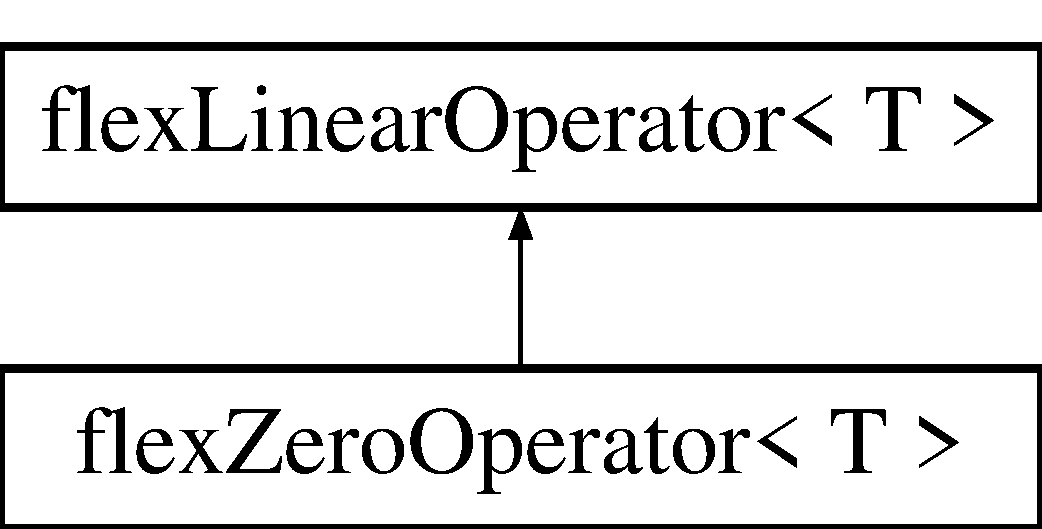
\includegraphics[height=2.000000cm]{classflex_zero_operator}
\end{center}
\end{figure}
\subsection*{Public Member Functions}
\begin{DoxyCompactItemize}
\item 
\hyperlink{classflex_zero_operator_a0d8f5246a460441e8ff71d6fe7359e23}{flex\+Zero\+Operator} (int a\+Num\+Rows, int a\+Num\+Cols, bool a\+Minus)
\begin{DoxyCompactList}\small\item\em initializes the zero operator \end{DoxyCompactList}\item 
\hyperlink{classflex_zero_operator}{flex\+Zero\+Operator}$<$ T $>$ $\ast$ \hyperlink{classflex_zero_operator_ab26ce548041980be572f7972907397af}{copy} ()
\begin{DoxyCompactList}\small\item\em copies the linear operator \end{DoxyCompactList}\item 
void \hyperlink{classflex_zero_operator_a3f512b2a67a803417d280e78418f8243}{times} (bool transposed, const Tdata \&input, Tdata \&output)
\begin{DoxyCompactList}\small\item\em applies linear operator on vector \end{DoxyCompactList}\item 
void \hyperlink{classflex_zero_operator_afad4cd5674474a1bc10224c99d72a65a}{times\+Plus} (bool transposed, const Tdata \&input, Tdata \&output)
\begin{DoxyCompactList}\small\item\em applies linear operator on vector and adds its result to y \end{DoxyCompactList}\item 
void \hyperlink{classflex_zero_operator_ae1b71503e1c6bf070deb080f2a0f1dd4}{times\+Minus} (bool transposed, const Tdata \&input, Tdata \&output)
\begin{DoxyCompactList}\small\item\em applies linear operator on vector and substracts its result from y \end{DoxyCompactList}\item 
T \hyperlink{classflex_zero_operator_a2c7b6c1cddc5a79c4d2948855a20b3f1}{get\+Max\+Row\+Sum\+Abs} (bool transposed)
\begin{DoxyCompactList}\small\item\em returns the maximum sum of absolute values per row used for preconditioning \end{DoxyCompactList}\item 
std\+::vector$<$ T $>$ \hyperlink{classflex_zero_operator_a4c9fbbcd1961590e2fabef75197f4367}{get\+Abs\+Row\+Sum} (bool transposed)
\begin{DoxyCompactList}\small\item\em returns a vector of sum of absolute values per row used for preconditioning \end{DoxyCompactList}\item 
thrust\+::device\+\_\+vector$<$ T $>$ \hyperlink{classflex_zero_operator_ad63f43f4b1abe71779e5b0ee364b93d1}{get\+Abs\+Row\+Sum\+C\+U\+DA} (bool transposed)
\begin{DoxyCompactList}\small\item\em same function as \hyperlink{classflex_zero_operator_a4c9fbbcd1961590e2fabef75197f4367}{get\+Abs\+Row\+Sum()} but implemented in C\+U\+DA \end{DoxyCompactList}\end{DoxyCompactItemize}
\subsection*{Additional Inherited Members}


\subsection{Detailed Description}
\subsubsection*{template$<$typename T$>$\newline
class flex\+Zero\+Operator$<$ T $>$}

represents a zero operator (empty matrix) 

\subsection{Constructor \& Destructor Documentation}
\mbox{\Hypertarget{classflex_zero_operator_a0d8f5246a460441e8ff71d6fe7359e23}\label{classflex_zero_operator_a0d8f5246a460441e8ff71d6fe7359e23}} 
\index{flex\+Zero\+Operator@{flex\+Zero\+Operator}!flex\+Zero\+Operator@{flex\+Zero\+Operator}}
\index{flex\+Zero\+Operator@{flex\+Zero\+Operator}!flex\+Zero\+Operator@{flex\+Zero\+Operator}}
\subsubsection{\texorpdfstring{flex\+Zero\+Operator()}{flexZeroOperator()}}
{\footnotesize\ttfamily template$<$typename T$>$ \\
\hyperlink{classflex_zero_operator}{flex\+Zero\+Operator}$<$ T $>$\+::\hyperlink{classflex_zero_operator}{flex\+Zero\+Operator} (\begin{DoxyParamCaption}\item[{int}]{a\+Num\+Rows,  }\item[{int}]{a\+Num\+Cols,  }\item[{bool}]{a\+Minus }\end{DoxyParamCaption})\hspace{0.3cm}{\ttfamily [inline]}}



initializes the zero operator 


\begin{DoxyParams}{Parameters}
{\em a\+Num\+Rows} & number of rows \\
\hline
{\em a\+Num\+Cols} & number of columns \\
\hline
{\em a\+Minus} & determines if operator is negated \\
\hline
\end{DoxyParams}
\begin{DoxySeeAlso}{See also}
\hyperlink{classflex_linear_operator_a7f986517e10aee21099ec7692b77905d}{is\+Minus} 
\end{DoxySeeAlso}


\subsection{Member Function Documentation}
\mbox{\Hypertarget{classflex_zero_operator_ab26ce548041980be572f7972907397af}\label{classflex_zero_operator_ab26ce548041980be572f7972907397af}} 
\index{flex\+Zero\+Operator@{flex\+Zero\+Operator}!copy@{copy}}
\index{copy@{copy}!flex\+Zero\+Operator@{flex\+Zero\+Operator}}
\subsubsection{\texorpdfstring{copy()}{copy()}}
{\footnotesize\ttfamily template$<$typename T$>$ \\
\hyperlink{classflex_zero_operator}{flex\+Zero\+Operator}$<$T$>$$\ast$ \hyperlink{classflex_zero_operator}{flex\+Zero\+Operator}$<$ T $>$\+::copy (\begin{DoxyParamCaption}{ }\end{DoxyParamCaption})\hspace{0.3cm}{\ttfamily [inline]}, {\ttfamily [virtual]}}



copies the linear operator 

\begin{DoxyReturn}{Returns}
copy of linear operator 
\end{DoxyReturn}


Implements \hyperlink{classflex_linear_operator_a7cc1425677cc30fcbd092ffd28d508c9}{flex\+Linear\+Operator$<$ T $>$}.

\mbox{\Hypertarget{classflex_zero_operator_a4c9fbbcd1961590e2fabef75197f4367}\label{classflex_zero_operator_a4c9fbbcd1961590e2fabef75197f4367}} 
\index{flex\+Zero\+Operator@{flex\+Zero\+Operator}!get\+Abs\+Row\+Sum@{get\+Abs\+Row\+Sum}}
\index{get\+Abs\+Row\+Sum@{get\+Abs\+Row\+Sum}!flex\+Zero\+Operator@{flex\+Zero\+Operator}}
\subsubsection{\texorpdfstring{get\+Abs\+Row\+Sum()}{getAbsRowSum()}}
{\footnotesize\ttfamily template$<$typename T$>$ \\
std\+::vector$<$T$>$ \hyperlink{classflex_zero_operator}{flex\+Zero\+Operator}$<$ T $>$\+::get\+Abs\+Row\+Sum (\begin{DoxyParamCaption}\item[{bool}]{transposed }\end{DoxyParamCaption})\hspace{0.3cm}{\ttfamily [inline]}, {\ttfamily [virtual]}}



returns a vector of sum of absolute values per row used for preconditioning 


\begin{DoxyParams}{Parameters}
{\em transposed} & is true if operator should be (temporarily) transposed before usage \\
\hline
\end{DoxyParams}
\begin{DoxyReturn}{Returns}
vector of sum of absolute values per row 
\end{DoxyReturn}


Implements \hyperlink{classflex_linear_operator_ad6caa7b09e6e3c401cadef61b8e2307e}{flex\+Linear\+Operator$<$ T $>$}.

\mbox{\Hypertarget{classflex_zero_operator_ad63f43f4b1abe71779e5b0ee364b93d1}\label{classflex_zero_operator_ad63f43f4b1abe71779e5b0ee364b93d1}} 
\index{flex\+Zero\+Operator@{flex\+Zero\+Operator}!get\+Abs\+Row\+Sum\+C\+U\+DA@{get\+Abs\+Row\+Sum\+C\+U\+DA}}
\index{get\+Abs\+Row\+Sum\+C\+U\+DA@{get\+Abs\+Row\+Sum\+C\+U\+DA}!flex\+Zero\+Operator@{flex\+Zero\+Operator}}
\subsubsection{\texorpdfstring{get\+Abs\+Row\+Sum\+C\+U\+D\+A()}{getAbsRowSumCUDA()}}
{\footnotesize\ttfamily template$<$typename T$>$ \\
thrust\+::device\+\_\+vector$<$T$>$ \hyperlink{classflex_zero_operator}{flex\+Zero\+Operator}$<$ T $>$\+::get\+Abs\+Row\+Sum\+C\+U\+DA (\begin{DoxyParamCaption}\item[{bool}]{transposed }\end{DoxyParamCaption})\hspace{0.3cm}{\ttfamily [inline]}, {\ttfamily [virtual]}}



same function as \hyperlink{classflex_zero_operator_a4c9fbbcd1961590e2fabef75197f4367}{get\+Abs\+Row\+Sum()} but implemented in C\+U\+DA 


\begin{DoxyParams}{Parameters}
{\em transposed} & is true if operator should be (temporarily) transposed before usage \\
\hline
\end{DoxyParams}
\begin{DoxyReturn}{Returns}
vector of sum of absolute values per row 
\end{DoxyReturn}


Implements \hyperlink{classflex_linear_operator_a0a0a431d43f4f9d36cbee0d31ba5a29b}{flex\+Linear\+Operator$<$ T $>$}.

\mbox{\Hypertarget{classflex_zero_operator_a2c7b6c1cddc5a79c4d2948855a20b3f1}\label{classflex_zero_operator_a2c7b6c1cddc5a79c4d2948855a20b3f1}} 
\index{flex\+Zero\+Operator@{flex\+Zero\+Operator}!get\+Max\+Row\+Sum\+Abs@{get\+Max\+Row\+Sum\+Abs}}
\index{get\+Max\+Row\+Sum\+Abs@{get\+Max\+Row\+Sum\+Abs}!flex\+Zero\+Operator@{flex\+Zero\+Operator}}
\subsubsection{\texorpdfstring{get\+Max\+Row\+Sum\+Abs()}{getMaxRowSumAbs()}}
{\footnotesize\ttfamily template$<$typename T$>$ \\
T \hyperlink{classflex_zero_operator}{flex\+Zero\+Operator}$<$ T $>$\+::get\+Max\+Row\+Sum\+Abs (\begin{DoxyParamCaption}\item[{bool}]{transposed }\end{DoxyParamCaption})\hspace{0.3cm}{\ttfamily [inline]}, {\ttfamily [virtual]}}



returns the maximum sum of absolute values per row used for preconditioning 


\begin{DoxyParams}{Parameters}
{\em transposed} & is true if operator should be (temporarily) transposed before usage \\
\hline
\end{DoxyParams}
\begin{DoxyReturn}{Returns}
maximum sum of absolute values per row 
\end{DoxyReturn}


Implements \hyperlink{classflex_linear_operator_afcb74697385ccb7c8d29870d7034c12a}{flex\+Linear\+Operator$<$ T $>$}.

\mbox{\Hypertarget{classflex_zero_operator_a3f512b2a67a803417d280e78418f8243}\label{classflex_zero_operator_a3f512b2a67a803417d280e78418f8243}} 
\index{flex\+Zero\+Operator@{flex\+Zero\+Operator}!times@{times}}
\index{times@{times}!flex\+Zero\+Operator@{flex\+Zero\+Operator}}
\subsubsection{\texorpdfstring{times()}{times()}}
{\footnotesize\ttfamily template$<$typename T$>$ \\
void \hyperlink{classflex_zero_operator}{flex\+Zero\+Operator}$<$ T $>$\+::times (\begin{DoxyParamCaption}\item[{bool}]{transposed,  }\item[{const Tdata \&}]{input,  }\item[{Tdata \&}]{output }\end{DoxyParamCaption})\hspace{0.3cm}{\ttfamily [inline]}, {\ttfamily [virtual]}}



applies linear operator on vector 

equals $ y = Ax $ 
\begin{DoxyParams}{Parameters}
{\em transposed} & is true if operator should be (temporarily) transposed before usage \\
\hline
{\em input} & data to be processed \\
\hline
{\em output} & output data \\
\hline
\end{DoxyParams}


Implements \hyperlink{classflex_linear_operator_a883982edf3be857815d2095e53f76e75}{flex\+Linear\+Operator$<$ T $>$}.

\mbox{\Hypertarget{classflex_zero_operator_ae1b71503e1c6bf070deb080f2a0f1dd4}\label{classflex_zero_operator_ae1b71503e1c6bf070deb080f2a0f1dd4}} 
\index{flex\+Zero\+Operator@{flex\+Zero\+Operator}!times\+Minus@{times\+Minus}}
\index{times\+Minus@{times\+Minus}!flex\+Zero\+Operator@{flex\+Zero\+Operator}}
\subsubsection{\texorpdfstring{times\+Minus()}{timesMinus()}}
{\footnotesize\ttfamily template$<$typename T$>$ \\
void \hyperlink{classflex_zero_operator}{flex\+Zero\+Operator}$<$ T $>$\+::times\+Minus (\begin{DoxyParamCaption}\item[{bool}]{transposed,  }\item[{const Tdata \&}]{input,  }\item[{Tdata \&}]{output }\end{DoxyParamCaption})\hspace{0.3cm}{\ttfamily [inline]}, {\ttfamily [virtual]}}



applies linear operator on vector and substracts its result from y 

equals $ y = y - Ax $ 
\begin{DoxyParams}{Parameters}
{\em transposed} & is true if operator should be (temporarily) transposed before usage \\
\hline
{\em input} & data to be processed \\
\hline
{\em output} & output data \\
\hline
\end{DoxyParams}


Implements \hyperlink{classflex_linear_operator_a62708874e134a649c8445df333079c69}{flex\+Linear\+Operator$<$ T $>$}.

\mbox{\Hypertarget{classflex_zero_operator_afad4cd5674474a1bc10224c99d72a65a}\label{classflex_zero_operator_afad4cd5674474a1bc10224c99d72a65a}} 
\index{flex\+Zero\+Operator@{flex\+Zero\+Operator}!times\+Plus@{times\+Plus}}
\index{times\+Plus@{times\+Plus}!flex\+Zero\+Operator@{flex\+Zero\+Operator}}
\subsubsection{\texorpdfstring{times\+Plus()}{timesPlus()}}
{\footnotesize\ttfamily template$<$typename T$>$ \\
void \hyperlink{classflex_zero_operator}{flex\+Zero\+Operator}$<$ T $>$\+::times\+Plus (\begin{DoxyParamCaption}\item[{bool}]{transposed,  }\item[{const Tdata \&}]{input,  }\item[{Tdata \&}]{output }\end{DoxyParamCaption})\hspace{0.3cm}{\ttfamily [inline]}, {\ttfamily [virtual]}}



applies linear operator on vector and adds its result to y 

equals $ y = y + Ax $ 
\begin{DoxyParams}{Parameters}
{\em transposed} & is true if operator should be (temporarily) transposed before usage \\
\hline
{\em input} & data to be processed \\
\hline
{\em output} & output data \\
\hline
\end{DoxyParams}


Implements \hyperlink{classflex_linear_operator_a3f2978ad1c5eae8cd4ae16deb2337416}{flex\+Linear\+Operator$<$ T $>$}.



The documentation for this class was generated from the following file\+:\begin{DoxyCompactItemize}
\item 
flex\+Zero\+Operator.\+h\end{DoxyCompactItemize}

\hypertarget{structflex_prox_dual_l2_inf_1_1_greater_equal_zero}{}\section{flex\+Prox\+Dual\+L2\+Inf$<$ T $>$\+:\+:Greater\+Equal\+Zero Struct Reference}
\label{structflex_prox_dual_l2_inf_1_1_greater_equal_zero}\index{flex\+Prox\+Dual\+L2\+Inf$<$ T $>$\+::\+Greater\+Equal\+Zero@{flex\+Prox\+Dual\+L2\+Inf$<$ T $>$\+::\+Greater\+Equal\+Zero}}
\subsection*{Public Member Functions}
\begin{DoxyCompactItemize}
\item 
\mbox{\Hypertarget{structflex_prox_dual_l2_inf_1_1_greater_equal_zero_a7542eeceded196cd2dbcaa4960228baa}\label{structflex_prox_dual_l2_inf_1_1_greater_equal_zero_a7542eeceded196cd2dbcaa4960228baa}} 
\+\_\+\+\_\+host\+\_\+\+\_\+ \+\_\+\+\_\+device\+\_\+\+\_\+ bool {\bfseries operator()} (T val)
\end{DoxyCompactItemize}


The documentation for this struct was generated from the following file\+:\begin{DoxyCompactItemize}
\item 
flex\+Prox\+Dual\+L2\+Inf.\+h\end{DoxyCompactItemize}

\hypertarget{structflex_prox_dual_l2_inf_1_1_l21_norm_dim2}{}\section{flex\+Prox\+Dual\+L2\+Inf$<$ T $>$\+:\+:L21\+Norm\+Dim2 Struct Reference}
\label{structflex_prox_dual_l2_inf_1_1_l21_norm_dim2}\index{flex\+Prox\+Dual\+L2\+Inf$<$ T $>$\+::\+L21\+Norm\+Dim2@{flex\+Prox\+Dual\+L2\+Inf$<$ T $>$\+::\+L21\+Norm\+Dim2}}
\subsection*{Public Member Functions}
\begin{DoxyCompactItemize}
\item 
\mbox{\Hypertarget{structflex_prox_dual_l2_inf_1_1_l21_norm_dim2_a9ba1b9bae488b5669f96f5eb9c66d7de}\label{structflex_prox_dual_l2_inf_1_1_l21_norm_dim2_a9ba1b9bae488b5669f96f5eb9c66d7de}} 
{\footnotesize template$<$typename Tuple $>$ }\\\+\_\+\+\_\+host\+\_\+\+\_\+ \+\_\+\+\_\+device\+\_\+\+\_\+ void {\bfseries operator()} (Tuple t)
\end{DoxyCompactItemize}


The documentation for this struct was generated from the following file\+:\begin{DoxyCompactItemize}
\item 
flex\+Prox\+Dual\+L2\+Inf.\+h\end{DoxyCompactItemize}

\hypertarget{structflex_prox_dual_l2_inf_1_1_l21_norm_dim3}{}\section{flex\+Prox\+Dual\+L2\+Inf$<$ T $>$\+:\+:L21\+Norm\+Dim3 Struct Reference}
\label{structflex_prox_dual_l2_inf_1_1_l21_norm_dim3}\index{flex\+Prox\+Dual\+L2\+Inf$<$ T $>$\+::\+L21\+Norm\+Dim3@{flex\+Prox\+Dual\+L2\+Inf$<$ T $>$\+::\+L21\+Norm\+Dim3}}
\subsection*{Public Member Functions}
\begin{DoxyCompactItemize}
\item 
\mbox{\Hypertarget{structflex_prox_dual_l2_inf_1_1_l21_norm_dim3_a82a8815b5e7798682f93400386b29f06}\label{structflex_prox_dual_l2_inf_1_1_l21_norm_dim3_a82a8815b5e7798682f93400386b29f06}} 
{\footnotesize template$<$typename Tuple $>$ }\\\+\_\+\+\_\+host\+\_\+\+\_\+ \+\_\+\+\_\+device\+\_\+\+\_\+ void {\bfseries operator()} (Tuple t)
\end{DoxyCompactItemize}


The documentation for this struct was generated from the following file\+:\begin{DoxyCompactItemize}
\item 
flex\+Prox\+Dual\+L2\+Inf.\+h\end{DoxyCompactItemize}

\hypertarget{structmy_abs_g_p_u}{}\section{my\+Abs\+G\+PU$<$ T $>$ Struct Template Reference}
\label{structmy_abs_g_p_u}\index{my\+Abs\+G\+P\+U$<$ T $>$@{my\+Abs\+G\+P\+U$<$ T $>$}}


thrust functor for calculating the absolute value of vector  




{\ttfamily \#include $<$tools.\+h$>$}

\subsection*{Public Member Functions}
\begin{DoxyCompactItemize}
\item 
\mbox{\Hypertarget{structmy_abs_g_p_u_a4db26700d95cd83aef0d16ac4b09b7ba}\label{structmy_abs_g_p_u_a4db26700d95cd83aef0d16ac4b09b7ba}} 
\+\_\+\+\_\+host\+\_\+\+\_\+ \+\_\+\+\_\+device\+\_\+\+\_\+ T {\bfseries operator()} (T x) const
\end{DoxyCompactItemize}


\subsection{Detailed Description}
\subsubsection*{template$<$typename T$>$\newline
struct my\+Abs\+G\+P\+U$<$ T $>$}

thrust functor for calculating the absolute value of vector 

The documentation for this struct was generated from the following file\+:\begin{DoxyCompactItemize}
\item 
\hyperlink{tools_8h}{tools.\+h}\end{DoxyCompactItemize}

\hypertarget{class_timer}{}\section{Timer Class Reference}
\label{class_timer}\index{Timer@{Timer}}


class for timing execution times  




{\ttfamily \#include $<$tools.\+h$>$}

\subsection*{Public Member Functions}
\begin{DoxyCompactItemize}
\item 
\mbox{\Hypertarget{class_timer_a9020542d73357a4eef512eefaf57524b}\label{class_timer_a9020542d73357a4eef512eefaf57524b}} 
void \hyperlink{class_timer_a9020542d73357a4eef512eefaf57524b}{reset} ()
\begin{DoxyCompactList}\small\item\em resets or starts the timer \end{DoxyCompactList}\item 
\mbox{\Hypertarget{class_timer_accef2f2b25869fbca2947a56b494d2a0}\label{class_timer_accef2f2b25869fbca2947a56b494d2a0}} 
void \hyperlink{class_timer_accef2f2b25869fbca2947a56b494d2a0}{end} ()
\begin{DoxyCompactList}\small\item\em ends the timer \end{DoxyCompactList}\item 
double \hyperlink{class_timer_a6a89a613c2af9b0d1e5f7e4ba9e46c54}{elapsed} () const
\begin{DoxyCompactList}\small\item\em returns the duration \end{DoxyCompactList}\end{DoxyCompactItemize}


\subsection{Detailed Description}
class for timing execution times 

\hyperlink{class_timer}{Timer} is a class for measuring execution times of the primal dual algorithm. It uses std\+::chrono and additionally cuda\+Device\+Synchronize() if the C\+U\+DA version of Flex\+Box has been compiled. 

\subsection{Member Function Documentation}
\mbox{\Hypertarget{class_timer_a6a89a613c2af9b0d1e5f7e4ba9e46c54}\label{class_timer_a6a89a613c2af9b0d1e5f7e4ba9e46c54}} 
\index{Timer@{Timer}!elapsed@{elapsed}}
\index{elapsed@{elapsed}!Timer@{Timer}}
\subsubsection{\texorpdfstring{elapsed()}{elapsed()}}
{\footnotesize\ttfamily double Timer\+::elapsed (\begin{DoxyParamCaption}{ }\end{DoxyParamCaption}) const\hspace{0.3cm}{\ttfamily [inline]}}



returns the duration 

returns the duration between \hyperlink{class_timer_a9020542d73357a4eef512eefaf57524b}{reset()} and \hyperlink{class_timer_accef2f2b25869fbca2947a56b494d2a0}{end()} in seconds (as double) or 0.\+0 if timer has not been stopped \begin{DoxyReturn}{Returns}
duration in seconds 
\end{DoxyReturn}


The documentation for this class was generated from the following file\+:\begin{DoxyCompactItemize}
\item 
\hyperlink{tools_8h}{tools.\+h}\end{DoxyCompactItemize}

\hypertarget{structvector_add_vector_times_vector_g_p_u}{}\section{vector\+Add\+Vector\+Times\+Vector\+G\+PU Struct Reference}
\label{structvector_add_vector_times_vector_g_p_u}\index{vector\+Add\+Vector\+Times\+Vector\+G\+PU@{vector\+Add\+Vector\+Times\+Vector\+G\+PU}}


thrust functor for elemntwise multiplication of two vectors following a summation of the result on a third vector  




{\ttfamily \#include $<$tools.\+h$>$}

\subsection*{Public Member Functions}
\begin{DoxyCompactItemize}
\item 
\mbox{\Hypertarget{structvector_add_vector_times_vector_g_p_u_abaad725feda316fd2ae3263793e6dfaa}\label{structvector_add_vector_times_vector_g_p_u_abaad725feda316fd2ae3263793e6dfaa}} 
\+\_\+\+\_\+host\+\_\+\+\_\+ \+\_\+\+\_\+device\+\_\+\+\_\+ {\bfseries vector\+Add\+Vector\+Times\+Vector\+G\+PU} (const int sign\+Rule)
\item 
\mbox{\Hypertarget{structvector_add_vector_times_vector_g_p_u_a6860a5fa42b72e7c20f4b2afa71a7ec9}\label{structvector_add_vector_times_vector_g_p_u_a6860a5fa42b72e7c20f4b2afa71a7ec9}} 
{\footnotesize template$<$typename Tuple $>$ }\\\+\_\+\+\_\+host\+\_\+\+\_\+ \+\_\+\+\_\+device\+\_\+\+\_\+ void {\bfseries operator()} (Tuple t)
\end{DoxyCompactItemize}
\subsection*{Public Attributes}
\begin{DoxyCompactItemize}
\item 
\mbox{\Hypertarget{structvector_add_vector_times_vector_g_p_u_ae1572bdebd4a20096ad76a7fc2956e2d}\label{structvector_add_vector_times_vector_g_p_u_ae1572bdebd4a20096ad76a7fc2956e2d}} 
const int {\bfseries sign\+Rule}
\end{DoxyCompactItemize}


\subsection{Detailed Description}
thrust functor for elemntwise multiplication of two vectors following a summation of the result on a third vector 

The documentation for this struct was generated from the following file\+:\begin{DoxyCompactItemize}
\item 
\hyperlink{tools_8h}{tools.\+h}\end{DoxyCompactItemize}

\chapter{File Documentation}
\hypertarget{tools_8h}{}\section{tools.\+h File Reference}
\label{tools_8h}\index{tools.\+h@{tools.\+h}}
\subsection*{Classes}
\begin{DoxyCompactItemize}
\item 
class \hyperlink{class_timer}{Timer}
\begin{DoxyCompactList}\small\item\em class for timing execution times \end{DoxyCompactList}\item 
struct \hyperlink{structmy_abs_g_p_u}{my\+Abs\+G\+P\+U$<$ T $>$}
\begin{DoxyCompactList}\small\item\em thrust functor for calculating the absolute value of vector \end{DoxyCompactList}\item 
struct \hyperlink{struct_k_lprojection_data_g_p_u}{K\+Lprojection\+Data\+G\+P\+U$<$ T $>$}
\item 
struct \hyperlink{structvector_add_vector_times_vector_g_p_u}{vector\+Add\+Vector\+Times\+Vector\+G\+PU}
\begin{DoxyCompactList}\small\item\em thrust functor for elemntwise multiplication of two vectors following a summation of the result on a third vector \end{DoxyCompactList}\end{DoxyCompactItemize}
\subsection*{Enumerations}
\begin{DoxyCompactItemize}
\item 
\mbox{\Hypertarget{tools_8h_ab8be8fa992a31c15058261e81ef8ba9d}\label{tools_8h_ab8be8fa992a31c15058261e81ef8ba9d}} 
enum \hyperlink{tools_8h_ab8be8fa992a31c15058261e81ef8ba9d}{my\+Sign} \{ {\bfseries P\+L\+US}, 
{\bfseries M\+I\+N\+US}, 
{\bfseries E\+Q\+U\+A\+LS}, 
{\bfseries C\+O\+M\+P\+O\+SE}
 \}\begin{DoxyCompactList}\small\item\em enum representing the type of concatenation \end{DoxyCompactList}
\item 
\mbox{\Hypertarget{tools_8h_aa34fd4f0962337a24e898ac0abdfff22}\label{tools_8h_aa34fd4f0962337a24e898ac0abdfff22}} 
enum \hyperlink{tools_8h_aa34fd4f0962337a24e898ac0abdfff22}{prox} \{ \newline
{\bfseries primal\+Empty\+Prox}, 
{\bfseries dual\+L1\+Aniso\+Prox}, 
{\bfseries dual\+L1\+Iso\+Prox}, 
{\bfseries dual\+L2\+Prox}, 
\newline
{\bfseries dual\+Frobenius\+Prox}, 
{\bfseries dual\+Huber\+Prox}, 
{\bfseries dual\+L2\+Data\+Prox}, 
{\bfseries dual\+L1\+Data\+Prox}, 
\newline
{\bfseries dual\+K\+L\+Data\+Prox}, 
{\bfseries dual\+Box\+Constraint\+Prox}, 
{\bfseries dual\+Inner\+Product\+Prox}
 \}\begin{DoxyCompactList}\small\item\em enum representing the type of prox \end{DoxyCompactList}
\item 
\mbox{\Hypertarget{tools_8h_a3fc67a2f9370c09fecbd90da67687d36}\label{tools_8h_a3fc67a2f9370c09fecbd90da67687d36}} 
enum \hyperlink{tools_8h_a3fc67a2f9370c09fecbd90da67687d36}{lin\+Op} \{ \newline
{\bfseries linear\+Op}, 
{\bfseries diagonal\+Op}, 
{\bfseries gradient\+Op}, 
{\bfseries identity\+Op}, 
\newline
{\bfseries matrix\+Op}, 
{\bfseries matrix\+G\+P\+U\+Op}, 
{\bfseries zero\+Op}, 
{\bfseries superpixel\+Op}, 
\newline
{\bfseries concat\+Op}
 \}\begin{DoxyCompactList}\small\item\em enum representing the type of a linear operator \end{DoxyCompactList}
\item 
\mbox{\Hypertarget{tools_8h_a40b3c158323c8bcb80e2095f3473213c}\label{tools_8h_a40b3c158323c8bcb80e2095f3473213c}} 
enum \hyperlink{tools_8h_a40b3c158323c8bcb80e2095f3473213c}{gradient\+Type} \{ {\bfseries forward}, 
{\bfseries backward}, 
{\bfseries central}
 \}\begin{DoxyCompactList}\small\item\em enum representing the type of gradient \end{DoxyCompactList}
\end{DoxyCompactItemize}
\subsection*{Functions}
\begin{DoxyCompactItemize}
\item 
\mbox{\Hypertarget{tools_8h_a216ffd5b7736c9ed15fb8738a3b60903}\label{tools_8h_a216ffd5b7736c9ed15fb8738a3b60903}} 
{\footnotesize template$<$typename T $>$ }\\T {\bfseries my\+Abs} (T x)
\item 
\mbox{\Hypertarget{tools_8h_a71b378ebdf9bc62a39108d5a30757076}\label{tools_8h_a71b378ebdf9bc62a39108d5a30757076}} 
{\footnotesize template$<$typename T $>$ }\\T {\bfseries my\+Min} (T a, T b)
\item 
\mbox{\Hypertarget{tools_8h_afda28a0b28aaac6e6e9be6c0488aee3a}\label{tools_8h_afda28a0b28aaac6e6e9be6c0488aee3a}} 
{\footnotesize template$<$typename T $>$ }\\T {\bfseries my\+Max} (T a, T b)
\item 
\mbox{\Hypertarget{tools_8h_a347fe37bf882cc1be3efe68082ffbd12}\label{tools_8h_a347fe37bf882cc1be3efe68082ffbd12}} 
double {\bfseries pow2} (double x)
\item 
\mbox{\Hypertarget{tools_8h_ad40f0e4b2cd494315cd6dddcf26afeef}\label{tools_8h_ad40f0e4b2cd494315cd6dddcf26afeef}} 
float {\bfseries pow2} (float x)
\item 
\mbox{\Hypertarget{tools_8h_a7b9f56b81e329d055c38a9056217f336}\label{tools_8h_a7b9f56b81e329d055c38a9056217f336}} 
{\footnotesize template$<$typename T $>$ }\\T {\bfseries vector\+Product} (const std\+::vector$<$ T $>$ \&v)
\item 
\mbox{\Hypertarget{tools_8h_a0ea5640424f56d4b1a6b33a4a30c4218}\label{tools_8h_a0ea5640424f56d4b1a6b33a4a30c4218}} 
{\footnotesize template$<$typename T $>$ }\\T {\bfseries vector\+Sum} (const std\+::vector$<$ T $>$ \&v)
\item 
\mbox{\Hypertarget{tools_8h_a9a624331066f771d67486345ecaabb1f}\label{tools_8h_a9a624331066f771d67486345ecaabb1f}} 
float {\bfseries vector\+Max} (std\+::vector$<$ float $>$ \&v)
\item 
\mbox{\Hypertarget{tools_8h_ae31fe4ccd5002a1efd0bf7e4678ce742}\label{tools_8h_ae31fe4ccd5002a1efd0bf7e4678ce742}} 
{\footnotesize template$<$typename T $>$ }\\void {\bfseries vector\+Scalar\+Product} (std\+::vector$<$ T $>$ \&v, T scalar\+Value)
\item 
\mbox{\Hypertarget{tools_8h_afca0d71e8db787c5163428382e86d266}\label{tools_8h_afca0d71e8db787c5163428382e86d266}} 
void {\bfseries vector\+Scalar\+Set} (std\+::vector$<$ float $>$ \&v, const float scalar\+Value)
\item 
\mbox{\Hypertarget{tools_8h_a7cb74d0cb2a66778ce71e089d3a9f03f}\label{tools_8h_a7cb74d0cb2a66778ce71e089d3a9f03f}} 
void {\bfseries vector\+Plus} (std\+::vector$<$ float $>$ \&v1, std\+::vector$<$ float $>$ \&v2)
\item 
\mbox{\Hypertarget{tools_8h_a27a4ca3fc1ca7328c3d9fcb9f36264a1}\label{tools_8h_a27a4ca3fc1ca7328c3d9fcb9f36264a1}} 
void {\bfseries vector\+Minus} (std\+::vector$<$ float $>$ \&v1, std\+::vector$<$ float $>$ \&v2)
\item 
\mbox{\Hypertarget{tools_8h_af7a41c43ce5bf2074604398647960508}\label{tools_8h_af7a41c43ce5bf2074604398647960508}} 
{\footnotesize template$<$typename T $>$ }\\void {\bfseries vector\+Abs} (std\+::vector$<$ T $>$ \&v)
\item 
\mbox{\Hypertarget{tools_8h_a0c9dcb7310f17fa86327b77319e125bf}\label{tools_8h_a0c9dcb7310f17fa86327b77319e125bf}} 
{\footnotesize template$<$typename T $>$ }\\void {\bfseries do\+Overrelaxation} (std\+::vector$<$ T $>$ \&x, std\+::vector$<$ T $>$ \&x\+Old, std\+::vector$<$ T $>$ \&x\+Bar)
\item 
\mbox{\Hypertarget{tools_8h_a587baf2e94ef5f64d5ea202da78cfbb4}\label{tools_8h_a587baf2e94ef5f64d5ea202da78cfbb4}} 
{\footnotesize template$<$typename T $>$ }\\void {\bfseries vector\+Pow2} (std\+::vector$<$ T $>$ \&v)
\item 
\mbox{\Hypertarget{tools_8h_aaf4e65c50cc69dff00258f68b1bafe1f}\label{tools_8h_aaf4e65c50cc69dff00258f68b1bafe1f}} 
{\footnotesize template$<$typename T $>$ }\\void {\bfseries vector\+Add\+Vector\+Times\+Vector} (std\+::vector$<$ T $>$ \&result, const std\+::vector$<$ T $>$ \&v1, const std\+::vector$<$ T $>$ \&v2, const int sign\+Rule)
\item 
\mbox{\Hypertarget{tools_8h_aa16a7793273712d18ccbf6818a8d2f2c}\label{tools_8h_aa16a7793273712d18ccbf6818a8d2f2c}} 
{\footnotesize template$<$typename T $>$ }\\void {\bfseries calculate\+X\+Y\+Error} (thrust\+::device\+\_\+vector$<$ T $>$ \&x, thrust\+::device\+\_\+vector$<$ T $>$ \&x\+Old, thrust\+::device\+\_\+vector$<$ T $>$ \&x\+Error, T tau)
\item 
\mbox{\Hypertarget{tools_8h_a914b03eb8abe5c53b659c620da617f79}\label{tools_8h_a914b03eb8abe5c53b659c620da617f79}} 
{\footnotesize template$<$typename T $>$ }\\\+\_\+\+\_\+host\+\_\+\+\_\+ \+\_\+\+\_\+device\+\_\+\+\_\+ T {\bfseries my\+Pow2\+G\+PU} (T x)
\item 
\mbox{\Hypertarget{tools_8h_ac67a4a6587b7e32f4437b6329ba7ff9e}\label{tools_8h_ac67a4a6587b7e32f4437b6329ba7ff9e}} 
{\footnotesize template$<$typename T $>$ }\\void {\bfseries vector\+Abs} (thrust\+::device\+\_\+vector$<$ T $>$ \&v)
\item 
\mbox{\Hypertarget{tools_8h_a2c68e60268912a3303b1ddcba63a2a4c}\label{tools_8h_a2c68e60268912a3303b1ddcba63a2a4c}} 
{\footnotesize template$<$typename T $>$ }\\\+\_\+\+\_\+host\+\_\+\+\_\+ \+\_\+\+\_\+device\+\_\+\+\_\+ T {\bfseries my\+Min\+G\+PU} (T a, T b)
\item 
\mbox{\Hypertarget{tools_8h_a09088267774b151caeca41e2b1ae7a3b}\label{tools_8h_a09088267774b151caeca41e2b1ae7a3b}} 
\+\_\+\+\_\+device\+\_\+\+\_\+ float {\bfseries my\+Min\+G\+P\+Uf} (float a, float b)
\item 
\mbox{\Hypertarget{tools_8h_a54e3c28a97bb7fb896ab60dd9bb1d23c}\label{tools_8h_a54e3c28a97bb7fb896ab60dd9bb1d23c}} 
\+\_\+\+\_\+device\+\_\+\+\_\+ float {\bfseries my\+Max\+G\+P\+Uf} (float a, float b)
\item 
\mbox{\Hypertarget{tools_8h_a0fe08c60dac2893a829cb1e237d95be5}\label{tools_8h_a0fe08c60dac2893a829cb1e237d95be5}} 
{\footnotesize template$<$typename T $>$ }\\\+\_\+\+\_\+host\+\_\+\+\_\+ \+\_\+\+\_\+device\+\_\+\+\_\+ T {\bfseries my\+Max\+G\+PU} (T a, T b)
\item 
\mbox{\Hypertarget{tools_8h_af4c900063f26acbd5f2f24e6f67d8705}\label{tools_8h_af4c900063f26acbd5f2f24e6f67d8705}} 
{\footnotesize template$<$typename T $>$ }\\T {\bfseries vector\+Sum} (thrust\+::device\+\_\+vector$<$ T $>$ \&v)
\item 
\mbox{\Hypertarget{tools_8h_ab8dc0c3410e8f30d27e449ec2ef1d09d}\label{tools_8h_ab8dc0c3410e8f30d27e449ec2ef1d09d}} 
{\footnotesize template$<$typename T $>$ }\\void {\bfseries vector\+Project\+K\+Ldata} (thrust\+::device\+\_\+vector$<$ T $>$ \&y, thrust\+::device\+\_\+vector$<$ T $>$ \&y\+Tilde, thrust\+::device\+\_\+vector$<$ T $>$ \&f, T alpha, T sigma)
\item 
\mbox{\Hypertarget{tools_8h_ad11cd46aad6d66463439efcd99b55d94}\label{tools_8h_ad11cd46aad6d66463439efcd99b55d94}} 
{\footnotesize template$<$typename T $>$ }\\void {\bfseries vector\+Scalar\+Set} (thrust\+::device\+\_\+vector$<$ T $>$ \&v, T scalar\+Value)
\item 
\mbox{\Hypertarget{tools_8h_aab6ab60a4247b8f82f2206ba6ab81b3c}\label{tools_8h_aab6ab60a4247b8f82f2206ba6ab81b3c}} 
{\footnotesize template$<$typename T $>$ }\\void {\bfseries vector\+Scalar\+Product} (thrust\+::device\+\_\+vector$<$ T $>$ \&v, const T scalar\+Value)
\item 
\mbox{\Hypertarget{tools_8h_a6153646012fb76f5f47b23b5bca194b0}\label{tools_8h_a6153646012fb76f5f47b23b5bca194b0}} 
{\footnotesize template$<$typename T $>$ }\\void {\bfseries vector\+Minus} (thrust\+::device\+\_\+vector$<$ T $>$ \&v1, thrust\+::device\+\_\+vector$<$ T $>$ \&v2)
\item 
\mbox{\Hypertarget{tools_8h_ae132dc76e79af67a86dd640558358b97}\label{tools_8h_ae132dc76e79af67a86dd640558358b97}} 
{\footnotesize template$<$typename T $>$ }\\void {\bfseries vector\+Add\+Squared} (thrust\+::device\+\_\+vector$<$ T $>$ \&v1, thrust\+::device\+\_\+vector$<$ T $>$ \&v2)
\item 
\mbox{\Hypertarget{tools_8h_a40c444535e8d1b69897981b24d498e31}\label{tools_8h_a40c444535e8d1b69897981b24d498e31}} 
{\footnotesize template$<$typename T $>$ }\\void {\bfseries vector\+Add\+Vector\+Times\+Vector} (thrust\+::device\+\_\+vector$<$ T $>$ \&result, const thrust\+::device\+\_\+vector$<$ T $>$ \&v1, const thrust\+::device\+\_\+vector$<$ T $>$ \&v2, const int sign\+Rule)
\item 
\mbox{\Hypertarget{tools_8h_a4dda1f2b70d5f24a679a2af8fcc8771e}\label{tools_8h_a4dda1f2b70d5f24a679a2af8fcc8771e}} 
{\footnotesize template$<$typename T $>$ }\\\+\_\+\+\_\+host\+\_\+\+\_\+ \+\_\+\+\_\+device\+\_\+\+\_\+ T {\bfseries sqrt\+G\+PU} (T x)
\item 
\mbox{\Hypertarget{tools_8h_a72f399d5f94ef2ac0230e76a92e00381}\label{tools_8h_a72f399d5f94ef2ac0230e76a92e00381}} 
{\footnotesize template$<$typename T $>$ }\\void {\bfseries vector\+Sqrt} (thrust\+::device\+\_\+vector$<$ T $>$ \&v1)
\item 
\mbox{\Hypertarget{tools_8h_a5484e298f09469e4c99e319c8c6b28d8}\label{tools_8h_a5484e298f09469e4c99e319c8c6b28d8}} 
{\footnotesize template$<$typename T $>$ }\\float {\bfseries vector\+Max} (thrust\+::device\+\_\+vector$<$ T $>$ \&v)
\end{DoxyCompactItemize}


\subsection{Detailed Description}
file containing global definitions and functions 
%--- End generated contents ---

% Bibliography
\newpage
\phantomsection
\bibliographystyle{plain}
\bibliography{bibTmpFile_1}
\addcontentsline{toc}{chapter}{Bibliography}

% Index
\backmatter
\newpage
\phantomsection
\clearemptydoublepage
\addcontentsline{toc}{chapter}{Index}
\printindex

\end{document}
